\clearpage
\bookpart{常微分方程}{Ordinary Differential Equations}
\label{part:ordinary-differential-equations}

\BookPartGuide{%
物体下落的速度、培养皿里细菌的数量、电路中的电流，这些量的变化规律往往比量本身更容易写下来。把“变化规律”和“起点”合在一起，就得到初值问题。本部分研究由导数与初值确定的曲线：能不能求出来，一定有解吗，解对数据有多敏感，算不出公式时怎样计算。

第~\ref{chap:ordinary-differential-equations}章从增长、冷却和运动进入，建立状态表示、解的检验和积分形式，并求解几类简单方程。第~\ref{chap:linear-differential-systems}章研究线性方程，用矩阵指数和状态转移矩阵把初值和外部输入变成可计算的响应。

后三章不再依赖解的公式。第~\ref{chap:ode-existence-continuation}章回答解是否存在、是否唯一、能延伸多远。第~\ref{chap:ode-sensitivity}章估计初值、参数和输入变化对有限时间解的影响，并由解的导数建立流映射和伴随表达。第~\ref{chap:ode-numerical-methods}章建立代表性的数值方法，分析误差如何累积，以及刚性和步长选择带来的问题。

本部分讨论有限时间内的解。解在长时间下趋向何处、吸引子与分岔等问题由卷九专门处理。}

\chapter{初值问题}
\label{chap:ordinary-differential-equations}

一杯刚泡好的咖啡放在桌上，温度一分一分降下来。我们说不出十分钟后它恰好多少度，却能说出降温的规律：咖啡比室温高得越多，降得越快。培养液中的细菌、摆动的钟摆也是这样，“此刻变化得多快”往往比“此刻是多少”更容易写下来。

规律不足以确定曲线。同样的降温规律，从$80$度出发和从$50$度出发是两条不同的曲线，所以还要告诉方程从哪里开始。规律加起点，就是本章的对象\term{初值问题}（initial value problem）。

把规律和起点合在一起之后，马上有几个具体问题。需要记录哪些量，才足以预测未来？钟摆只知道角度够不够？一个算出来的公式，凭什么算作解，它在哪段时间上才是解？能求出公式的方程有哪几类，变形时会不会丢掉解？暖气在某一刻突然关闭，方程右端出现跳变，解又该怎样理解？

全章沿着这几个问题走。第~\ref{sec:ivp-equations}节用增长和冷却分开规律与初值，第~\ref{sec:ivp-state}节用钟摆说明状态要包含哪些量。第~\ref{sec:ivp-verification}节规定什么曲线算解，并检查解的定义区间。第~\ref{sec:ivp-first-order}节求解两类一阶方程。第~\ref{sec:ivp-integral}节把方程改写成累积形式，第~\ref{sec:ivp-measurable}节用这个形式处理不连续的输入。

\section{方程与初值}
\label{sec:ivp-equations}

一条未知曲线怎样被“变化规律”和“起点”确定下来？先看两个增长的例子，再看冷却，然后把共同的结构写成定义。

\paragraph{指数增长}
设$x(t)$是培养液中细菌的数量（以某个单位计），$t$是时间。营养充足时，每个细菌在单位时间内分裂的机会相同，所以单位时间的增量与现有数量成正比，比例系数记作$r>0$：
\begin{equation}
 \dot{x}(t)=r\,x(t).
 \label{eq:ivp-exponential}
\end{equation}
字母上方的点表示对时间$t$求导，$\dot{x}(t)=\mathrm{d}x/\mathrm{d}t$，两个点表示二阶导数$\ddot{x}$。式~\eqref{eq:ivp-exponential}没有告诉我们$x(t)$是多少，只告诉我们每个时刻曲线的斜率与当时的高度之比是$r$。

我们知道指数函数的导数还是它自己乘以系数，所以对任意常数$C$，曲线$x(t)=C\mathrm{e}^{rt}$都满足式~\eqref{eq:ivp-exponential}。一条规律对应一族曲线。要从中选出一条，需要再说明某个时刻的数量。若$t=0$时数量为$x_0$，代入得$C=x_0$，于是
\begin{equation}
 x(t)=x_0\mathrm{e}^{rt}.
 \label{eq:ivp-exponential-solution}
\end{equation}

\paragraph{饱和增长}
营养有限时，数量越接近培养液能养活的上限$K$，每个细菌分裂得越慢。最简单的写法是把比例系数$r$改成$r(1-x/K)$：
\begin{equation}
 \dot{x}=r\,x\Bigl(1-\frac{x}{K}\Bigr).
 \label{eq:ivp-logistic-general}
\end{equation}
这个方程称为\term{Logistic方程}（logistic equation）。把数量的单位取成$K$，把时间的单位取成$1/r$，就可以令$K=1$，$r=1$，得到本章贯穿使用的形式：
\begin{equation}
 \dot{x}=x(1-x).
 \label{eq:ivp-logistic}
\end{equation}

$x$很小时，因子$1-x$接近$1$，式~\eqref{eq:ivp-logistic}与$\dot{x}=x$几乎相同。取$x_0=0.1$，两个方程在$t=0$的斜率分别是$0.09$和$0.1$。从$x_0=0.1$出发，式~\eqref{eq:ivp-logistic}的解是
\begin{equation}
 x(t)=\frac{\mathrm{e}^{t}}{9+\mathrm{e}^{t}},
 \label{eq:ivp-logistic-solution}
\end{equation}
它怎么得来是第~\ref{sec:ivp-separable}小节的内容，满足方程的验算在第~\ref{sec:ivp-verification}节。在$t=\ln 9\approx 2.197$时，它等于$0.5$；同一时刻指数增长已经到了$0.1\times 9=0.9$。

\paragraph{方向场}
式~\eqref{eq:ivp-logistic}的右端是一个二元的“斜率表”：给定点$(t,x)$，它给出曲线经过这一点时应有的斜率。在平面上取许多点，每点画一小段具有该斜率的线段，得到的图称为\term{方向场}（direction field）。

图~\ref{fig:ivp-growth-laws}比较了两种增长的方向场。(a)中线段的倾斜程度只随高度增加，越往上越陡，曲线一路加速。(b)中线段在$x=0.5$附近最陡，接近$x=1$时变平，超过$1$后转而向下，曲线被压向$x=1$。两幅图里三条曲线的规律相同，只是起点不同。

\begin{BookInlineFigure}
 \centering
 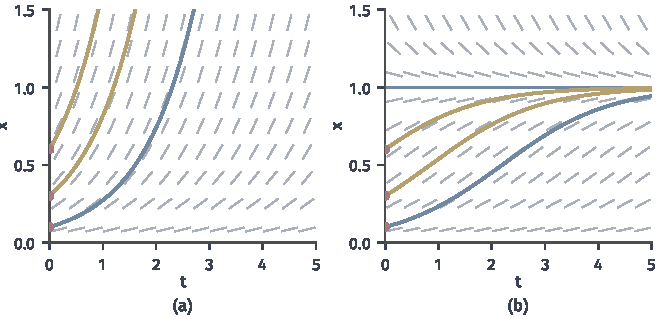
\includegraphics[width=112mm]{figures/06-differential-equations/01-ordinary-differential-equations/matplotlib/ivp-growth-laws/figure.pdf}
 \caption{同一规律、不同初值。灰色短线是方向场，每段的斜率等于右端在该点的值。(a)指数增长$\dot{x}=x$。(b)饱和增长$\dot{x}=x(1-x)$。红点是初值$x_0=0.1,\,0.3,\,0.6$，蓝线是$x_0=0.1$的解，黄线是另两个初值的解。(b)中的水平蓝线$x\equiv 1$也是解。}
 \label{fig:ivp-growth-laws}
\end{BookInlineFigure}

可以把方向场想象成平面上的水流。时间总把水往右推，竖直方向的流速由右端决定。把一片小木片放在初始点上，它漂过的路径就是解曲线。这个比喻说明了两件事：解处处与线段相切，换一个投放点就换一条路径。比喻也有局限：真实的水流中一片木片只走一条路，方程却未必如此，第~\ref{sec:ivp-separable}小节会遇到从同一点分出多条解的例子。

\paragraph{冷却}
第三个例子让规律中出现环境的数据。设$x(t)$是咖啡的温度，室温恒为$c$度。Newton冷却定律假设降温速率与温差成正比，比例系数$k>0$由杯子和空气决定：
\begin{equation}
 \dot{x}=-k(x-c).
 \label{eq:ivp-cooling}
\end{equation}
令$y=x-c$，则$\dot{y}=\dot{x}=-ky$，这是式~\eqref{eq:ivp-exponential}取$r=-k$的情形。由式~\eqref{eq:ivp-exponential-solution}，$y(t)=y_0\mathrm{e}^{-kt}$，换回温度得到
\begin{equation}
 x(t)=c+(x_0-c)\mathrm{e}^{-kt}.
 \label{eq:ivp-cooling-solution}
\end{equation}

取$c=20$，$k=0.1$（每分钟），$x_0=80$。十分钟后温度为$20+60\mathrm{e}^{-1}\approx 42.07$度，此时的变化率是
\[
 \dot{x}(10)=-0.1\times(42.07-20)\approx -2.21,
\]
也就是每分钟下降约$2.21$度。图~\ref{fig:ivp-cooling-field}中紫色线段正是曲线在这一点的切线，它与周围的灰色短线方向一致。

\begin{BookInlineFigure}
 \centering
 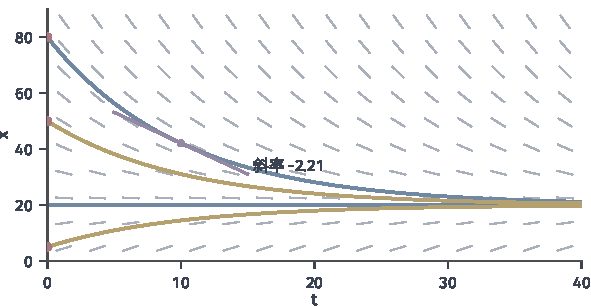
\includegraphics[width=100mm]{figures/06-differential-equations/01-ordinary-differential-equations/matplotlib/ivp-cooling-field/figure.pdf}
 \caption{冷却方程$\dot{x}=-0.1(x-20)$的方向场，时间以分钟计，温度以摄氏度计。蓝线从$80$度出发，黄线从$50$度和$5$度出发，水平蓝线是恒为室温的解。紫色线段是蓝线在$t=10$处的切线，斜率约为$-2.21$。}
 \label{fig:ivp-cooling-field}
\end{BookInlineFigure}

三个例子有共同的结构：一个已知的右端，一个未知的时间函数，一个指定的起点。这里还须说清未知函数定义在哪里，右端在哪里有意义，于是有下面的定义。

\begin{definition}[初值问题]
 \label{def:ivp-ivp}
 设$T\subseteq\mathbb{R}$是区间，$\bm{D}\subseteq\mathbb{R}^{n}$是开集，$\bm{f}:T\times\bm{D}\to\mathbb{R}^{n}$，$t_0\in T$，$\bm{x}_0\in\bm{D}$。\term{初值问题}是寻找一个包含$t_0$的非退化区间$I\subseteq T$，以及曲线$\bm{x}:I\to\bm{D}$，使
 \begin{equation}
 \dot{\bm{x}}(t)=\bm{f}\bigl(t,\bm{x}(t)\bigr),\quad t\in I,\qquad
 \bm{x}(t_0)=\bm{x}_0.
 \label{eq:ivp-ivp}
 \end{equation}
 $t$称为时间，$\bm{x}(t)\in\mathbb{R}^{n}$称为状态，$\bm{f}$称为右端，$t_0$称为初始时刻，$\bm{x}_0$称为\term{初值}（initial value），$I$称为解的\term{存在区间}（interval of existence）。
\end{definition}

“方程成立”的准确含义在第~\ref{sec:ivp-verification}节规定。这个定义中各个对象的地位不同。$\bm{f}$、$t_0$、$\bm{x}_0$、$T$、$\bm{D}$是给定的数据，曲线$\bm{x}$是未知量，存在区间$I$也是答案的一部分，事先并不知道它有多长。式~\eqref{eq:ivp-ivp}的第一式是规律，第二式是起点，缺一不可。标量情形$n=1$时，状态写成不加粗的$x(t)$，右端写成$f(t,x)$，上面的增长与冷却都属于这种情形。

\paragraph{微分方程的分类用语}
含有未知函数导数的等式称为\term{微分方程}（differential equation）。若未知函数只依赖一个自变量，称为\term{常微分方程}（ordinary differential equation，ODE）。方程中出现的最高导数的次数称为\term{阶}（order）。式~\eqref{eq:ivp-exponential}至式~\eqref{eq:ivp-cooling}都是一阶常微分方程。式~\eqref{eq:ivp-ivp}看起来只含一阶导数，下一节会说明高阶方程也能写成这个样子。

\paragraph{初值与两点边值}
初值的特点是所有条件都给在同一时刻。对比一个二阶方程：
\begin{equation}
 \ddot{x}+x=0,
 \label{eq:ivp-harmonic}
\end{equation}
它的解是$x(t)=a\cos t+b\sin t$，其中$a,b$是常数，下面直接代入即可验证：$\ddot{x}=-a\cos t-b\sin t=-x$。两个常数要由两个条件定出来，关键在于条件放在哪里。

若两个条件都放在$t=0$，即给定位置$x(0)=0$和速度$\dot{x}(0)=v$，代入得$a=0$，$b=v$，于是$x(t)=v\sin t$。无论$v$取什么，都恰好得到一条曲线，这就是图~\ref{fig:ivp-ivp-bvp}(a)。

若把条件放在区间的两端，要求$x(0)=0$，$x(\pi)=\beta$，就成了\term{两点边值问题}（two-point boundary value problem）。第一个条件仍给出$a=0$，第二个条件变成
\[
 b\sin\pi=\beta,\qquad\text{即}\qquad 0=\beta.
\]
所以$\beta\neq 0$时一条解也没有，$\beta=0$时每个$b$都给出一条解。图~\ref{fig:ivp-ivp-bvp}(b)中$x(\pi)=1.2$的空心点无法到达，而$x(\pi)=0$的红点被无穷多条曲线同时经过。

\begin{BookInlineFigure}
 \centering
 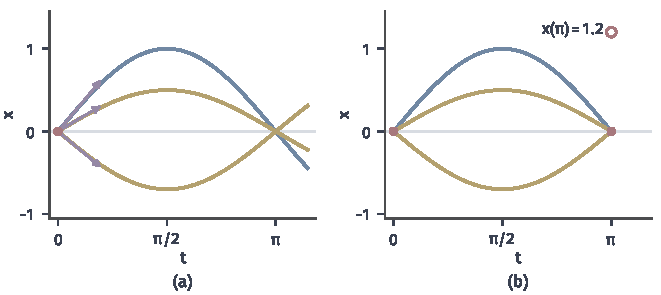
\includegraphics[width=112mm]{figures/06-differential-equations/01-ordinary-differential-equations/matplotlib/ivp-ivp-bvp/figure.pdf}
 \caption{方程$\ddot{x}+x=0$的两种提法。(a)初值问题：$x(0)=0$，紫色箭头表示初速度$v=1,\,0.5,\,-0.7$，每个初速度对应一条解$v\sin t$。(b)两点边值问题：两端红点$x(0)=x(\pi)=0$对应无穷多条解$b\sin t$，图中画出$b=1,\,0.5,\,-0.7$；空心点$x(\pi)=1.2$无解可达。}
 \label{fig:ivp-ivp-bvp}
\end{BookInlineFigure}

差别的根源在于计算的方式。初值问题的全部信息都在起点，可以沿时间一步步往前推。两点边值问题的条件分在两头，必须把整段曲线同时考虑，右端点的要求能否满足，还取决于方程本身。上面$\sin\pi=0$恰好使右端条件失去作用；若把区间长度换成$\pi/2$，条件变成$b=\beta$，解又唯一了。这类问题的一维例子由第~\ref{chap:elliptic-equations}章承接，本部分只讨论初值问题。

\section{状态表示}
\label{sec:ivp-state}

定义~\ref{def:ivp-ivp}只含一阶导数，而力学里的方程通常是二阶的。此刻的哪些量足以决定未来？回答这个问题，就能把高阶方程放进同一个框架，也能把时间、输入与状态分开。

\paragraph{摆只知道角度够不够}
图~\ref{fig:ivp-pendulum-diagram}是一个单摆。设摆长为$\ell$，$y(t)$是摆杆偏离竖直方向的角度（弧度），重力加速度记作$\gamma$。忽略阻力，重力沿圆弧切向的分量是$-\gamma\sin y$，切向加速度是$\ell\ddot{y}$，Newton第二定律给出
\begin{equation}
 \ddot{y}=-\kappa\sin y,\qquad\kappa=\frac{\gamma}{\ell}.
 \label{eq:ivp-pendulum}
\end{equation}
以下取时间单位使$\kappa=1$。

\begin{BookInlineFigure}
 \centering
 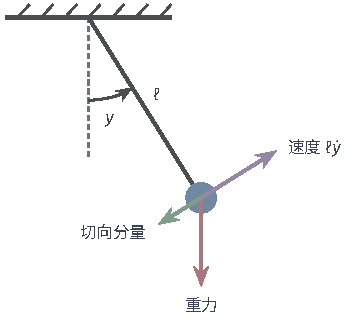
\includegraphics[width=60mm]{figures/06-differential-equations/01-ordinary-differential-equations/tikz/ivp-pendulum-diagram/figure.pdf}
 \caption{单摆的受力。$y$是摆杆与竖直方向的夹角，$\ell$是摆长。红色箭头是重力，绿色箭头是它沿圆弧切向的分量，紫色箭头是摆球的速度，大小为$\ell\lvert\dot{y}\rvert$。}
 \label{fig:ivp-pendulum-diagram}
\end{BookInlineFigure}

式~\eqref{eq:ivp-pendulum}给出的是加速度。只知道此刻的角度，能算出加速度，却算不出角度的变化率。同样在$y=1$的位置，摆球可能静止，也可能正在向上或向下运动，接下来的走向完全不同。图~\ref{fig:ivp-pendulum-state}(a)的三条曲线都从$y=1$出发，初始角速度分别是$0$、$1$和$-1$。

由此得到选择状态的原则：\term{状态}（state）是此刻的一组量，有了它和方程，下一瞬间的变化就完全确定，不需要回头查看历史。单摆需要角度和角速度两个量。令
\[
 x_1=y,\qquad x_2=\dot{y},
\]
则$\dot{x}_1=x_2$，而由式~\eqref{eq:ivp-pendulum}有$\dot{x}_2=-\sin x_1$。写成向量形式，
\begin{equation}
 \dot{\bm{x}}=\bm{f}(\bm{x})=\begin{pmatrix}x_2\\-\sin x_1\end{pmatrix},\qquad
 \bm{x}(0)=\begin{pmatrix}y(0)\\\dot{y}(0)\end{pmatrix}.
 \label{eq:ivp-pendulum-system}
\end{equation}
这就是定义~\ref{def:ivp-ivp}的形式，$n=2$。在状态$(1,0)$，右端是$(0,-\sin 1)\approx(0,-0.841)$：角度暂时不变，角速度开始变负。

\begin{BookInlineFigure}
 \centering
 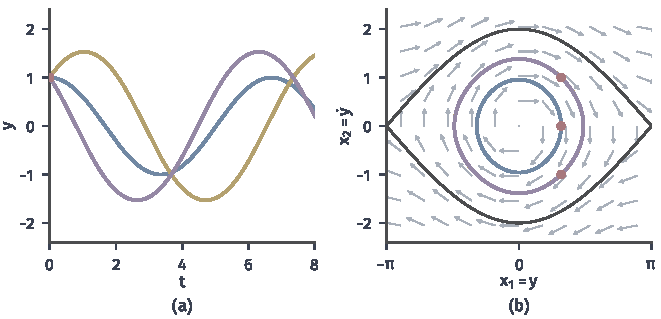
\includegraphics[width=112mm]{figures/06-differential-equations/01-ordinary-differential-equations/matplotlib/ivp-pendulum-state/figure.pdf}
 \caption{单摆$\ddot{y}=-\sin y$。三个初值都有$y(0)=1$，初始角速度为$0$（蓝）、$1$（黄）、$-1$（紫）。(a)角度随时间的变化。(b)相平面上的轨道：灰色箭头是右端的方向（长度已归一化），红点是初始状态，黄色和紫色的初始状态在同一条闭轨上。深灰色曲线$x_2=\pm 2\cos(x_1/2)$分开来回摆动与绕轴翻转两种运动。}
 \label{fig:ivp-pendulum-state}
\end{BookInlineFigure}

把$(x_1,x_2)$当作平面坐标，就得到图~\ref{fig:ivp-pendulum-state}(b)这样的\term{相平面}（phase plane）。每一点画一个箭头，表示状态在那一点的运动方向；解走过的路径称为\term{轨道}（orbit）。时间不再是坐标轴，而是沿轨道前进的快慢。这和方向场的区别在于：方向场的横轴是时间，所以一条解是从左往右的曲线；相平面没有时间轴，解可以绕回来。

相平面上的闭轨有一个可以手算的来源。定义$E=x_2^2/2+1-\cos x_1$，沿解求导，并用式~\eqref{eq:ivp-pendulum-system}代入：
\[
 \dot{E}=x_2\dot{x}_2+\sin x_1\,\dot{x}_1
 =x_2(-\sin x_1)+\sin x_1\,x_2=0.
\]
所以$E$沿解不变，解留在$E$的等值线上。三个初值的$E$分别是
\[
 E(1,0)=1-\cos 1\approx 0.460,\qquad E(1,\pm 1)=1.5-\cos 1\approx 0.960.
\]
后两个数相同，所以图中黄色与紫色的初值落在同一条闭轨上，只是位置不同。深灰色曲线对应$E=2$，也就是摆恰好能走到最高点的能量。

\paragraph{高阶方程化为一阶系统}
同样的做法适用于任意阶数。设标量未知函数$y$满足$m$阶方程
\begin{equation}
 y^{(m)}=h\bigl(t,y,\dot{y},\ldots,y^{(m-1)}\bigr).
 \label{eq:ivp-high-order}
\end{equation}
下一瞬间要知道的是$y$及其直到$m-1$阶的导数，所以令$x_j=y^{(j-1)}$，$j=1,\ldots,m$。这些量之间的关系如图~\ref{fig:ivp-state-chain}所示：前面每个分量的导数恰好是下一个分量，只有最后一个分量的导数由$h$决定。

\begin{BookInlineFigure}
 \centering
 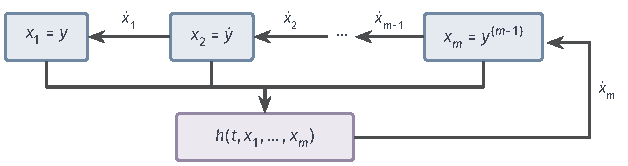
\includegraphics[width=106mm]{figures/06-differential-equations/01-ordinary-differential-equations/tikz/ivp-state-chain/figure.pdf}
 \caption{$m$阶方程的状态链。蓝框是状态的分量，水平箭头表示前一分量的导数等于后一分量，紫框由全部分量和时间算出最后一个分量的导数$\dot{x}_m$。}
 \label{fig:ivp-state-chain}
\end{BookInlineFigure}

\begin{lemma}[降阶]
 \label{lem:ivp-order-reduction}
 设$h$在$T\times\bm{D}$上有定义，$\bm{D}\subseteq\mathbb{R}^{m}$是开集，$I\subseteq T$是区间。函数$y:I\to\mathbb{R}$在$I$上$m$次可微且满足式~\eqref{eq:ivp-high-order}，并使$(y,\dot{y},\ldots,y^{(m-1)})$取值于$\bm{D}$，当且仅当
 \begin{equation}
 \bm{x}=\bigl(y,\dot{y},\ldots,y^{(m-1)}\bigr)
 \label{eq:ivp-reduction-state}
 \end{equation}
 在$I$上可微，取值于$\bm{D}$，并满足一阶系统$\dot{x}_j=x_{j+1}$（$j<m$），$\dot{x}_m=h(t,x_1,\ldots,x_m)$。
\end{lemma}

\begin{proof}
 若$y$满足式~\eqref{eq:ivp-high-order}，按定义~\eqref{eq:ivp-reduction-state}逐分量求导，前$m-1$个分量给出$\dot{x}_j=y^{(j)}=x_{j+1}$，最后一个分量给出
 \[
 \dot{x}_m=y^{(m)}=h(t,y,\ldots,y^{(m-1)})=h(t,x_1,\ldots,x_m).
 \]
 反过来，设一阶系统有可微解$\bm{x}$，令$y=x_1$。由$\dot{x}_1=x_2$，$y$可微且$\dot{y}=x_2$。$x_2$可微，所以$y$二次可微且$\ddot{y}=x_3$。依次进行到$x_m$，得到$y^{(m-1)}=x_m$，而$x_m$可微，于是$y$是$m$次可微的，并且$y^{(m)}=\dot{x}_m=h(t,y,\ldots,y^{(m-1)})$。
\end{proof}

相应的初值必须同时给出$y(t_0),\dot{y}(t_0),\ldots,y^{(m-1)}(t_0)$这$m$个数。$m$阶方程需要$m$个初始条件，道理就在这里。

下面用一个二阶方程走一遍。设
\[
 \ddot{y}+3\dot{y}+2y=\cos t,\qquad y(0)=1,\quad\dot{y}(0)=0.
\]
令$x_1=y$，$x_2=\dot{y}$，把二阶导数解出来，$\ddot{y}=\cos t-3\dot{y}-2y$，得到
\[
 \dot{\bm{x}}=\begin{pmatrix}0&1\\-2&-3\end{pmatrix}\bm{x}+\begin{pmatrix}0\\\cos t\end{pmatrix},\qquad
 \bm{x}(0)=\begin{pmatrix}1\\0\end{pmatrix}.
\]
这个系统的矩阵形式和解法由第~\ref{chap:linear-differential-systems}章给出。

\paragraph{状态、时间与外部输入}
上面的方程右端显含$\cos t$，它不是状态的一部分，而是外部施加的作用。给单摆加上阻力和一个随时间变化的驱动力矩$g(t)$，方程变成$\ddot{y}=-\sin y-c\dot{y}+g(t)$，其中$c\geq 0$是阻尼系数，状态方程是
\[
 \dot{x}_1=x_2,\qquad\dot{x}_2=-\sin x_1-cx_2+g(t).
\]
这里出现了三种不同地位的量：状态$(x_1,x_2)$由方程决定；驱动力矩$g$事先给定，不受状态影响；$c$是整段时间不变的常数。一般写法是图~\ref{fig:ivp-state-input-blocks}中的
\begin{equation}
 \dot{\bm{x}}=\bm{h}\bigl(\bm{x},\bm{g}(t),\bm{\theta}\bigr),
 \label{eq:ivp-input-system}
\end{equation}
其中$\bm{g}(t)$称为\term{外部输入}（external input），$\bm{\theta}$称为参数。

\begin{BookInlineFigure}
 \centering
 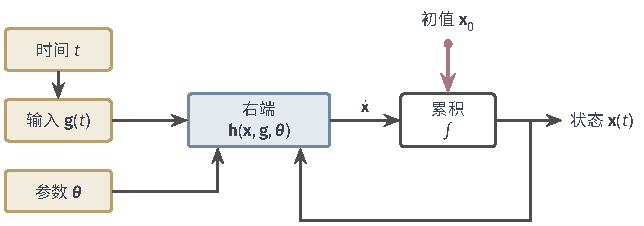
\includegraphics[width=109mm]{figures/06-differential-equations/01-ordinary-differential-equations/tikz/ivp-state-input-blocks/figure.pdf}
 \caption{状态方程的信息流。时间先决定输入，输入与参数同当前状态一起进入右端，得到变化率，再累积成状态，初值给累积的起点。状态沿反馈回路影响自己的变化率。}
 \label{fig:ivp-state-input-blocks}
\end{BookInlineFigure}

一旦$\bm{g}$和$\bm{\theta}$选定，就可以把它们代入右端，得到
\[
 \bm{f}(t,\bm{x})=\bm{h}\bigl(\bm{x},\bm{g}(t),\bm{\theta}\bigr),
\]
式~\eqref{eq:ivp-input-system}于是成为定义~\ref{def:ivp-ivp}的形式。时间$t$通过输入进入右端，所以$\bm{f}$显含时间。下面的表说明四种量的区别。

\begin{BookInlineTable}
 \centering
 \caption{初值问题中四种量的角色}
 \label{tab:ivp-roles}
 \begin{tabular}{lll}
 \toprule
 量 & 由谁决定 & 例子 \\
 \midrule
 时间$t$ & 自变量 & 钟面读数 \\
 状态$\bm{x}(t)$ & 由方程和初值决定 & 角度与角速度 \\
 外部输入$\bm{g}(t)$ & 事先给定的时间函数 & 驱动力矩 \\
 参数$\bm{\theta}$ & 事先给定的常数 & 阻尼系数$c$ \\
 \bottomrule
 \end{tabular}
\end{BookInlineTable}

分界并不是绝对的，要看问题怎么提。若力矩由当前角度算出，例如$g=-\beta x_1$，它就不再是事先给定的时间函数，而成了状态的函数，应当并入右端。

\paragraph{自治方程}
右端不显含时间的方程称为\term{自治方程}（autonomous equation），写作$\dot{\bm{x}}=\bm{f}(\bm{x})$，此时取$T=\mathbb{R}$；否则称为\term{非自治方程}（non-autonomous equation）。指数增长、饱和增长、冷却和无驱动的单摆都是自治的，$\dot{x}=\cos t$是非自治的。

自治意味着规律不随时间改变：今天和明天从同一状态出发，后面的故事相同，只是整体错开一段时间。

\begin{lemma}[自治方程的时间平移]
 \label{lem:ivp-time-shift}
 设$\bm{x}:I\to\bm{D}$满足$\dot{\bm{x}}=\bm{f}(\bm{x})$，$\tau\in\mathbb{R}$。则曲线$\tilde{\bm{x}}(t)=\bm{x}(t-\tau)$在平移后的区间$I+\tau$上也满足同一方程。
\end{lemma}

\begin{proof}
 由链式法则，$\dot{\tilde{\bm{x}}}(t)=\dot{\bm{x}}(t-\tau)$。再用方程在时刻$t-\tau$成立，得到
 \[
 \dot{\tilde{\bm{x}}}(t)=\bm{f}\bigl(\bm{x}(t-\tau)\bigr)=\bm{f}\bigl(\tilde{\bm{x}}(t)\bigr).
 \]
\end{proof}

图~\ref{fig:ivp-time-shift}对比了平移的结果，平移量都是$\tau=1.5$。(a)中方向场沿水平方向不变，黄线是蓝线向右平移的结果，依然处处与线段相切。(b)中方程是$\dot{x}=\cos t$，解$x=\sin t$平移后是$\sin(t-1.5)$，它的导数$\cos(t-1.5)$不等于右端$\cos t$，黄线穿过方向场的线段。

\begin{BookInlineFigure}
 \centering
 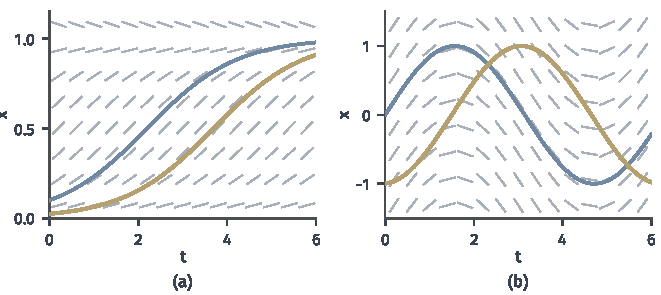
\includegraphics[width=112mm]{figures/06-differential-equations/01-ordinary-differential-equations/matplotlib/ivp-time-shift/figure.pdf}
 \caption{时间平移。蓝线是解，黄线是蓝线向右平移$1.5$的结果。(a)自治方程$\dot{x}=x(1-x)$：方向场沿时间方向不变，平移后仍是解。(b)非自治方程$\dot{x}=\cos t$：方向场随$t$变化，平移后不再与线段相切。}
 \label{fig:ivp-time-shift}
\end{BookInlineFigure}

\paragraph{用扩充状态消去显含时间}
非自治方程可以改写成自治方程，做法是把时间也当作一个状态分量。引入新分量$s$，规定$\dot{s}=1$，$s(t_0)=t_0$。扩充后的状态$\bm{z}=(\bm{x},s)\in\mathbb{R}^{n+1}$满足
\begin{equation}
 \dot{\bm{z}}=\bm{F}(\bm{z})=\begin{pmatrix}\bm{f}(s,\bm{x})\\1\end{pmatrix},\qquad
 \bm{z}(t_0)=\begin{pmatrix}\bm{x}_0\\t_0\end{pmatrix}.
 \label{eq:ivp-extended-state}
\end{equation}
这个系统的右端不显含$t$。由$\dot{s}=1$和初值，$s(t)=t_0+(t-t_0)=t$，所以$\bm{f}(s,\bm{x})$恰好就是$\bm{f}(t,\bm{x})$，式~\eqref{eq:ivp-extended-state}的前$n$个分量与原方程相同。反过来，原方程的解$\bm{x}$连同$s(t)=t$就是式~\eqref{eq:ivp-extended-state}的解。两个问题的解一一对应。

这个改写解释了状态的含义为什么要包括时间。取受迫振子$\ddot{y}+y=\cos 3t$，初值$y(0)=0.175$，$\dot{y}(0)=0.2$，解是$y(t)=0.3\cos t+0.2\sin t-\tfrac{1}{8}\cos 3t$。在$(x_1,x_2)=(y,\dot{y})$平面上，这条轨线在$t\approx 2.335$和$t\approx 3.027$经过同一点$(-0.157,-0.107)$，而两个时刻的右端分别约为
\[
 (-0.107,\ 0.908),\qquad(-0.107,\ -0.784).
\]
方向不同，说明只看$(x_1,x_2)$不足以决定下一瞬间的变化。图~\ref{fig:ivp-extended-lift}(b)把时间$s$加为第三个坐标，这两个时刻分到了不同的高度，交点随之消失。

\begin{BookInlineFigure}
 \centering
 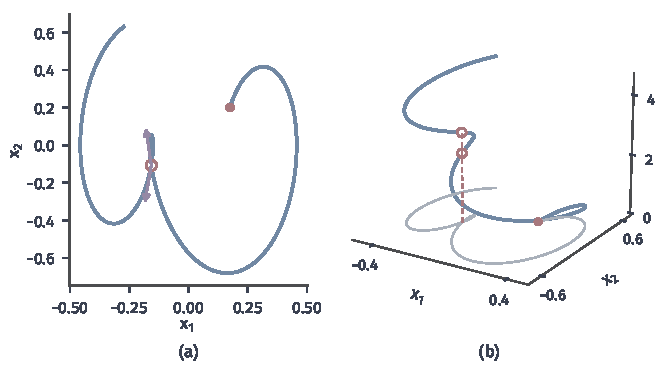
\includegraphics[width=112mm]{figures/06-differential-equations/01-ordinary-differential-equations/matplotlib/ivp-extended-lift/figure.pdf}
 \caption{受迫振子$\ddot{y}+y=\cos 3t$的轨线，$0\leq t\leq 4.6$。(a)在$(x_1,x_2)$平面上自交于空心点，紫色箭头是两个时刻右端的方向，红点是初值。(b)加入坐标$s=t$后，蓝线的两个对应点高度不同，灰线是它在底面上的投影。}
 \label{fig:ivp-extended-lift}
\end{BookInlineFigure}

改写是有代价的。维数增加一维；$\dot{s}=1$永不为零，所以扩充系统没有不动的状态；时间对右端的影响变成了状态对右端的影响，若$\bm{f}$对时间只有很差的正则性，$\bm{F}$对状态分量$s$的正则性也一样差。第~\ref{sec:ivp-measurable}节会看到这一点的后果。

\section{解的检验}
\label{sec:ivp-verification}

经过一番代数整理，得到了$x^2+t^2=1$这样的关系，问题解决了吗？这只是一个等式，还不是一条定义在某个区间上的曲线。在讨论任何求解方法之前，先规定一条曲线要满足什么才算解。

\begin{definition}[经典解]
 \label{def:ivp-classical-solution}
 考虑定义~\ref{def:ivp-ivp}的初值问题。设$I\subseteq T$是包含$t_0$的非退化区间，曲线$\bm{x}:I\to\bm{D}$在$I$的每一点可微（区间端点属于$I$时取单侧导数）。若
 \begin{equation}
 \dot{\bm{x}}(t)=\bm{f}\bigl(t,\bm{x}(t)\bigr)\quad\text{对每个}t\in I\text{成立，}\qquad
 \bm{x}(t_0)=\bm{x}_0,
 \label{eq:ivp-classical-solution}
 \end{equation}
 则称$\bm{x}$是初值问题在$I$上的\term{经典解}（classical solution），其图像称为\term{解曲线}（solution curve）。
\end{definition}

这个定义要求核对四件事。第一，定义域是一个区间，不能是几段分开的时间。第二，$\bm{x}(t)$始终留在$\bm{D}$中，右端处处有定义。第三，方程在区间的每一点成立，不只是在初始时刻。第四，初值成立。若$\bm{f}$连续，复合函数$t\mapsto\bm{f}(t,\bm{x}(t))$也连续，由方程可知$\dot{\bm{x}}$连续，此时经典解自动连续可微。

用这四条来验算式~\eqref{eq:ivp-logistic-solution}。函数$x(t)=\mathrm{e}^{t}/(9+\mathrm{e}^{t})$在整个实轴上有定义，分母恒正，所以取$I=\mathbb{R}$。按商的求导法则，
\[
 \dot{x}(t)=\frac{\mathrm{e}^{t}(9+\mathrm{e}^{t})-\mathrm{e}^{t}\mathrm{e}^{t}}{(9+\mathrm{e}^{t})^2}
 =\frac{9\mathrm{e}^{t}}{(9+\mathrm{e}^{t})^2}.
\]
另一方面，把$x(t)$代入右端，先算$1-x=9/(9+\mathrm{e}^{t})$，于是
\[
 x(1-x)=\frac{\mathrm{e}^{t}}{9+\mathrm{e}^{t}}\cdot\frac{9}{9+\mathrm{e}^{t}}
 =\frac{9\mathrm{e}^{t}}{(9+\mathrm{e}^{t})^2}.
\]
两式相同，方程成立。又$x(0)=1/10$，初值成立。这里$\bm{D}=\mathbb{R}$，取值范围没有限制。

\paragraph{隐式公式需要选支和定区间}
考虑$\dot{x}=-t/x$，$x(0)=1$。这里$T=\mathbb{R}$，右端在$x=0$处没有定义，所以取$D=(0,\infty)$，初值$1$落在其中。把方程写成$x\dot{x}=-t$，两边都是全导数：
\[
 \frac{\mathrm{d}}{\mathrm{d}t}\Bigl(\frac{x^2}{2}\Bigr)=-t.
\]
积分并代入初值，得到隐式关系
\begin{equation}
 x^2+t^2=1.
 \label{eq:ivp-implicit-circle}
\end{equation}

式~\eqref{eq:ivp-implicit-circle}是图~\ref{fig:ivp-implicit-branches}中的整个圆，它在每个$t\in(-1,1)$上有两个$x$，不是一条曲线。初值选中上半支$x=\sqrt{1-t^2}$。在$(-1,1)$上$x>0$，直接求导：
\[
 \dot{x}=\frac{-t}{\sqrt{1-t^2}}=-\frac{t}{x},
\]
方程成立，解的存在区间是$I=(-1,1)$。下半支从$x(0)=-1$出发，属于$D=(-\infty,0)$上的另一个初值问题，不能接在上半支后面。

\begin{BookInlineFigure}
 \centering
 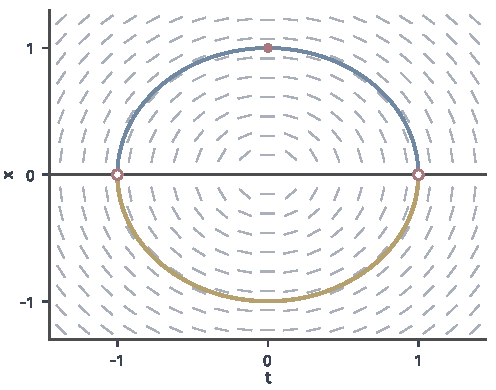
\includegraphics[width=84mm]{figures/06-differential-equations/01-ordinary-differential-equations/matplotlib/ivp-implicit-branches/figure.pdf}
 \caption{$\dot{x}=-t/x$的隐式解$x^2+t^2=1$。深灰色直线$x=0$上右端没有定义，把平面分成两部分。红点是初值$x(0)=1$，它选中蓝色上半支；黄色下半支是另一个初值问题的解。空心点处切线竖直，解不能延伸到端点$t=\pm 1$。}
 \label{fig:ivp-implicit-branches}
\end{BookInlineFigure}

端点$t=\pm 1$也不属于存在区间。那里$x=0$，已经离开了$D$；从公式看，$\sqrt{1-t^2}$在$t=\pm 1$的导数也不存在。解的存在区间比公式的“定义范围”$[-1,1]$小，这正是定义中第二条和第三条要求的结果。

\paragraph{平衡解}
第二种容易被漏掉的解是常值解。对$\dot{x}=x(1-x)$，右端在$x=0$和$x=1$处为零，所以常值函数$x\equiv 0$和$x\equiv 1$满足方程：左边的导数为零，右边也为零。

一般地，若$\bm{x}^{\star}\in\bm{D}$对每个$t\in T$都满足$\bm{f}(t,\bm{x}^{\star})=\bm{0}$，则常值曲线$\bm{x}(t)\equiv\bm{x}^{\star}$是从$\bm{x}^{\star}$出发的解，称为\term{平衡解}（equilibrium solution）。它的存在区间是整个$T$。第~\ref{sec:ivp-separable}小节的求解过程要除以右端的因子，平衡解正好落在被除掉的位置。例如式~\eqref{eq:ivp-logistic}的非平衡解可以用一个常数$C$统一写成下面的公式，这样的公式称为\term{通解}（general solution）：
\[
 x(t)=\frac{1}{1+C\mathrm{e}^{-t}},
\]
$C=0$给出$x\equiv 1$，但没有任何有限的$C$能给出$x\equiv 0$。用通解公式来核对“解是否都找到了”时，这样的解需要单独列出。

\paragraph{有限时间爆炸}
第三种现象是公式本身完全正常，解却走不到远处。考虑$\dot{x}=x^2$，$x(0)=1$。曲线$x(t)=1/(1-t)$的导数是
\[
 \dot{x}(t)=\frac{1}{(1-t)^2}=x(t)^2,
\]
并且$x(0)=1$。这是经典解，但它只在$t<1$时有意义：当$t$从左侧趋于$1$时，$x(t)\to+\infty$。这种现象称为\term{有限时间爆炸}（finite-time blow-up）。

右端$x^2$是处处光滑的函数，没有任何奇异之处，爆炸完全来自增长本身。翻倍时间可以说明它和指数增长的差别。由解的公式，$x_0=1$的解到达高度$x$的时刻是$t=1-1/x$。于是从$x=a$涨到$x=2a$需要的时间是
\[
 \frac{1}{2a}=\Bigl(1-\frac{1}{2a}\Bigr)-\Bigl(1-\frac{1}{a}\Bigr).
\]
从$1$开始，依次翻倍所需时间是$1/2,1/4,1/8,\ldots$，总和是$1$，这正是爆炸时刻。指数增长$\dot{x}=x$每次翻倍都需要$\ln 2$的时间，翻倍无穷多次要无穷长的时间。

\begin{BookInlineFigure}
 \centering
 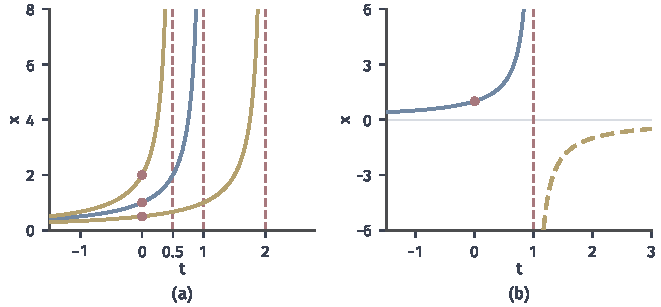
\includegraphics[width=112mm]{figures/06-differential-equations/01-ordinary-differential-equations/matplotlib/ivp-blow-up/figure.pdf}
 \caption{$\dot{x}=x^2$的有限时间爆炸。(a)初值$x_0=1$（蓝）与$x_0=0.5,\,2$（黄）的解$x=x_0/(1-x_0t)$，红色虚线是爆炸时刻$1/x_0$。初值越大，爆炸越早。(b)公式$1/(1-t)$在$t>1$还有一支（黄色虚线），它与蓝线被$t=1$隔开，也不经过初值，不属于这个初值问题的解。}
 \label{fig:ivp-blow-up}
\end{BookInlineFigure}

对一般初值$x_0>0$，解是$x=x_0/(1-x_0t)$，存在区间是$(-\infty,1/x_0)$，图~\ref{fig:ivp-blow-up}(a)显示爆炸时刻依赖于初值。这是非线性方程的特点：同一个方程，不同初值的解活得长短不同，存在区间事先无法从方程上直接读出来。

公式$1/(1-t)$在$t>1$时也有值，而且也满足微分等式。但图~\ref{fig:ivp-blow-up}(b)中右侧的那一支从负无穷升上来，与初值所在的那一支被$t=1$隔开，不在同一个区间上，所以不是我们的解。“解的存在区间是区间”这一要求在这里起作用。

\paragraph{检查清单}
把上面三个例子收拢起来。拿到一个候选公式时，依次回答下表中的问题；前两行决定存在区间，后两行决定它确实是解。

\begin{BookInlineTable}
 \centering
 \caption{候选解的检查项}
 \label{tab:ivp-checklist}
 \begin{tabular}{ll}
 \toprule
 检查项 & 对应的例子 \\
 \midrule
 是否是定义在一个区间上的函数 & 圆$x^2+t^2=1$要选支 \\
 状态是否留在右端的定义域内 & $\dot{x}=-t/x$要求$x\neq 0$ \\
 该区间内的每一点方程是否成立 & $1/(1-t)$只取$t<1$的一支 \\
 初值是否成立，是否漏掉平衡解 & $x\equiv 0$不在通解公式中 \\
 \bottomrule
 \end{tabular}
\end{BookInlineTable}

这张表只用来检验一条给定的曲线。它不回答“还有没有别的解”，也不回答“解最长能延伸到哪里”，这两个问题由第~\ref{chap:ode-existence-continuation}章回答。

\section{一阶方程的解析求解}
\label{sec:ivp-first-order}

有了解的标准，就可以着手求解。多数方程写不出公式，能够求解的方程靠的是右端的特殊形式：或者时间与状态可以分开，或者换一个未知量后可以分开。下面两小节分别处理这两种情况。一阶线性方程的积分因子在第~\ref{chap:linear-differential-systems}章统一介绍。

\subsection{分离变量}
\label{sec:ivp-separable}

若右端是时间的函数与状态的函数的乘积，
\begin{equation}
 \dot{x}=a(t)\,b(x),
 \label{eq:ivp-separable}
\end{equation}
则称方程为\term{可分离方程}（separable equation）。这里$a:T\to\mathbb{R}$连续，$b:D\to\mathbb{R}$连续，$T$是区间，$D$是开区间。

\paragraph{从形式计算到定理}
教科书里常见的写法是把方程改写成$\mathrm{d}x/b(x)=a(t)\,\mathrm{d}t$，再两边积分。这个写法方便记忆，却藏着两个问题：除以$b(x)$要求$b(x)\neq 0$；积分之后得到的是一个等式，把$x$解出来还需要函数可逆。下面的定理把这两点写清楚。

\begin{theorem}[分离变量]
 \label{thm:ivp-separation}
 考虑式~\eqref{eq:ivp-separable}与初值$x(t_0)=x_0$，$t_0\in T$，$x_0\in D$。
 \begin{enumerate}
 \item 若$b(x_0)=0$，则常值函数$x\equiv x_0$是$T$上的解。
 \item 若$b(x_0)\neq 0$，记$D_0\subseteq D$为包含$x_0$且$b$在其上无零点的最大开区间，定义
 \begin{equation}
 B(x)=\int_{x_0}^{x}\frac{\mathrm{d}\xi}{b(\xi)},\quad x\in D_0,\qquad
 A(t)=\int_{t_0}^{t}a(s)\,\mathrm{d}s,\quad t\in T.
 \label{eq:ivp-separation-primitives}
 \end{equation}
 则$B$是$D_0$上严格单调的连续可微函数，其值域$J=B(D_0)$是包含$0$的开区间。对任何包含$t_0$的区间$I\subseteq T$，只要$A(I)\subseteq J$，函数
 \begin{equation}
 x(t)=B^{-1}\bigl(A(t)\bigr)
 \label{eq:ivp-separation-solution}
 \end{equation}
 就是$I$上的解；并且$I$上任何取值于$D_0$的解都等于式~\eqref{eq:ivp-separation-solution}。
 \end{enumerate}
\end{theorem}

\begin{proof}
 第一条可直接验证：常值函数导数为零，而右端$a(t)b(x_0)=0$。

 下面证第二条。在$D_0$上$b$连续且无零点，由介值定理$b$不变号，所以$1/b$连续且不变号。由微积分基本定理，$B$连续可微，$B'=1/b$，于是$B$严格单调。严格单调的连续函数把开区间映成开区间，又$B(x_0)=0$，所以$0\in J$。

 反函数$B^{-1}:J\to D_0$连续可微，导数为$1/B'$，即
 \[
 (B^{-1})'(y)=b\bigl(B^{-1}(y)\bigr).
 \]
 若$A(I)\subseteq J$，由链式法则，式~\eqref{eq:ivp-separation-solution}定义的$x$满足
 \[
 \dot{x}(t)=b\bigl(B^{-1}(A(t))\bigr)\,\dot{A}(t)=b\bigl(x(t)\bigr)\,a(t).
 \]
 又$x(t_0)=B^{-1}(0)=x_0$，所以$x$是解。

 反过来，设$x:I\to D_0$是任意解。由链式法则，
 \[
 \frac{\mathrm{d}}{\mathrm{d}t}B\bigl(x(t)\bigr)=\frac{\dot{x}(t)}{b(x(t))}=a(t).
 \]
 右端连续，从$t_0$积分，得到$B(x(t))-B(x_0)=A(t)$，即$B(x(t))=A(t)$。这说明$A(I)\subseteq J$，并且$x(t)=B^{-1}(A(t))$。
\end{proof}

定理的条件各有用处。$a$、$b$连续保证$A$、$B$有定义。$D_0$的选取把$x_0$所在的一段状态与$b$的零点隔开，保证能除。条件$A(I)\subseteq J$决定存在区间：式~\eqref{eq:ivp-separation-solution}只在$A(t)$落在$J$中时有意义。最后一句中的“取值于$D_0$”是一个实际的限制，解是否会离开$D_0$，要看$b$在$D_0$端点附近的行为，本小节末尾再讨论。

\paragraph{Logistic方程的完整求解}
对式~\eqref{eq:ivp-logistic}，$a\equiv 1$，$b(x)=x(1-x)$，$t_0=0$。$b$的零点是$0$和$1$，它们给出两个平衡解，并把实轴分成三段：$(-\infty,0)$、$(0,1)$、$(1,\infty)$。$x_0$落在哪一段，$D_0$就是哪一段。

先把被积函数拆成部分分式：
\[
 \frac{1}{\xi(1-\xi)}=\frac{1}{\xi}+\frac{1}{1-\xi}.
\]
在每一段上$\xi/(1-\xi)$保持固定符号，逐项积分得到
\[
 B(x)=\Bigl[\ln\Bigl\lvert\frac{\xi}{1-\xi}\Bigr\rvert\Bigr]_{x_0}^{x}
 =\ln\frac{x(1-x_0)}{x_0(1-x)}.
\]
这里$A(t)=t$，令$B(x)=t$并解出$x$：
\begin{equation}
 x(t)=\frac{x_0\mathrm{e}^{t}}{1-x_0+x_0\mathrm{e}^{t}}.
 \label{eq:ivp-logistic-general-solution}
\end{equation}
代入$x_0=0.1$，分子分母同乘$10$，就得到式~\eqref{eq:ivp-logistic-solution}。

公式相同，存在区间却随初值而不同。定理告诉我们，存在区间由$J$决定，所以只要算出$B$的值域。取$x_0=2$，$D_0=(1,\infty)$，这时
\[
 B(x)=\ln\frac{x}{2(x-1)}.
\]
当$x\to 1^{+}$时$B\to+\infty$，当$x\to+\infty$时$B\to-\ln 2$，所以$J=(-\ln 2,\infty)$，存在区间是$I=(-\ln 2,\infty)$。类似地，取$x_0=-0.5$，$D_0=(-\infty,0)$，
\[
 B(x)=\ln\frac{3x}{x-1}.
\]
当$x\to 0^{-}$时$B\to-\infty$，当$x\to-\infty$时$B\to\ln 3$，所以$J=(-\infty,\ln 3)$，$I=(-\infty,\ln 3)$。

\begin{BookInlineTable}
 \centering
 \caption{Logistic方程$\dot{x}=x(1-x)$的三种初值}
 \label{tab:ivp-logistic-regimes}
 \begin{tabular}{llll}
 \toprule
 初值$x_0$ & $D_0$ & $J=B(D_0)$ & 存在区间$I$ \\
 \midrule
 $0.1$ & $(0,1)$ & $\mathbb{R}$ & $\mathbb{R}$ \\
 $2$ & $(1,\infty)$ & $(-\ln 2,\infty)$ & $(-\ln 2,\infty)$ \\
 $-0.5$ & $(-\infty,0)$ & $(-\infty,\ln 3)$ & $(-\infty,\ln 3)$ \\
 \bottomrule
 \end{tabular}
\end{BookInlineTable}

图~\ref{fig:ivp-logistic-regimes}画出了这三条解。在$x_0=2$的解上，往回追溯，在$t=-\ln 2$之前状态是无穷大；在$x_0=-0.5$的解上，$t$增加到$\ln 3$时状态趋于$-\infty$。右侧的竖线称为相线，它把自治标量方程的信息压缩到状态轴上：两个点是平衡解，箭头表示状态运动的方向，方向由$b(x)$的符号决定。

\begin{BookInlineFigure}
 \centering
 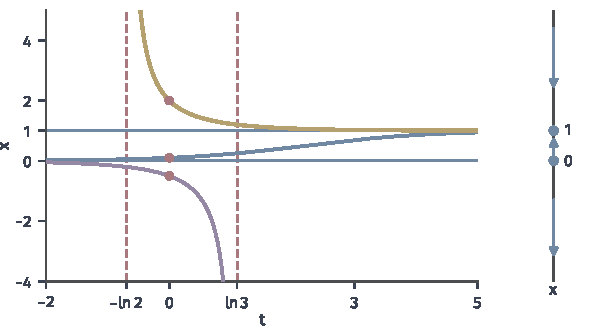
\includegraphics[width=104mm]{figures/06-differential-equations/01-ordinary-differential-equations/matplotlib/ivp-logistic-regimes/figure.pdf}
 \caption{$\dot{x}=x(1-x)$的三类解。蓝线$x_0=0.1$的解在全实轴上存在，黄线$x_0=2$的解在$t\downarrow-\ln 2$时趋于$+\infty$，紫线$x_0=-0.5$的解在$t\uparrow\ln 3$时趋于$-\infty$。水平蓝线是平衡解$x\equiv 0$与$x\equiv 1$，红色虚线是两个爆炸时刻。右侧相线上的箭头是$\dot{x}$的符号。}
 \label{fig:ivp-logistic-regimes}
\end{BookInlineFigure}

\paragraph{$a(t)$是一个改了刻度的时钟}
时间因子$a(t)$的作用可以这样看。令$\chi(s)$是自治方程$\chi'=b(\chi)$的解，$\chi(0)=x_0$，这个解由定理（取$a\equiv 1$）给出，满足$B(\chi(s))=s$。比较式~\eqref{eq:ivp-separation-solution}，有$x(t)=\chi(A(t))$。也就是说，时间因子只是把自治解放到一个新的时钟$s=A(t)$上走，时钟的快慢由$a(t)$决定，$a(t)<0$时时钟倒着走。

例如$\dot{x}=2tx^2$，$x(0)=1$。这里$a(t)=2t$，$b(x)=x^2$，$D_0=(0,\infty)$，计算得
\[
 A(t)=t^2,\qquad B(x)=1-\frac{1}{x},\qquad J=(-\infty,1).
\]
由$B(x)=A(t)$解出$x=1/(1-t^2)$，条件$A(t)\in J$即$t^2<1$，存在区间是$(-1,1)$。这正是第~\ref{sec:ivp-verification}节的爆炸解$1/(1-s)$放到时钟$s=t^2$上。代回检验：$\dot{x}=2t/(1-t^2)^2=2tx^2$，$x(0)=1$。

\paragraph{隐式解什么时候解得出}
积分后得到的是$B(x)=A(t)$，它未必能写成初等函数。考虑
\[
 \dot{x}=\frac{2t}{1+\mathrm{e}^{x}},\qquad x(0)=0.
\]
这里$a(t)=2t$，$b(x)=1/(1+\mathrm{e}^{x})$无零点，$D_0=\mathbb{R}$。计算两个原函数：
\[
 B(x)=\int_0^{x}(1+\mathrm{e}^{\xi})\,\mathrm{d}\xi=x+\mathrm{e}^{x}-1,\qquad A(t)=t^2.
\]
于是解由$x+\mathrm{e}^{x}-1=t^2$确定，这个方程没有初等的解出形式。但$B$严格递增，值域是整个$\mathbb{R}$，定理保证对每个$t$都恰有一个$x$，解在全实轴上存在。$t=1$时要解$x+\mathrm{e}^{x}=2$，数值求根得$x\approx 0.443$，这是图~\ref{fig:ivp-implicit-solve}中的紫点。

\begin{BookInlineFigure}
 \centering
 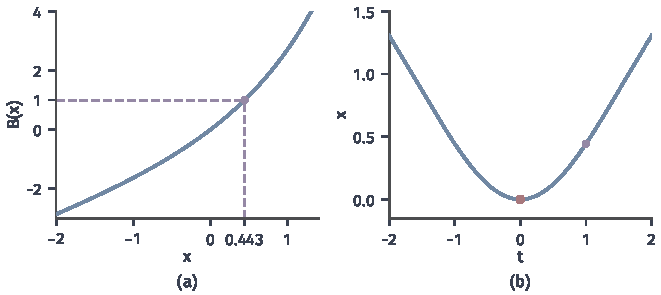
\includegraphics[width=112mm]{figures/06-differential-equations/01-ordinary-differential-equations/matplotlib/ivp-implicit-solve/figure.pdf}
 \caption{隐式解$x+\mathrm{e}^{x}-1=t^2$。(a)函数$B(x)=x+\mathrm{e}^{x}-1$严格递增，水平线$B=1$（$t=\pm 1$时的$A(t)$）与曲线恰交于一点，$x\approx 0.443$。(b)由此逐点解出的解曲线，红点是初值$x(0)=0$，紫点对应$t=1$。}
 \label{fig:ivp-implicit-solve}
\end{BookInlineFigure}

更一般地，积分可能给出一个形如$G(t,x)=C$的关系。在一点附近能把$x$解成$t$的函数，靠的是隐函数定理的条件$\partial_x G\neq 0$，可参考\BookChapterRef{chap:implicit-inverse-functions}{卷二第22章“隐函数与反函数”}。对分离变量，$G(t,x)=B(x)-A(t)$，所以$\partial_xG=1/b(x)\neq 0$，这就是定理中$B$可逆的原因。圆$x^2+t^2=1$对应的$G=x^2+t^2$在$t=\pm 1$处$\partial_xG=2x=0$，解在那里走不下去，与图~\ref{fig:ivp-implicit-branches}一致。

\paragraph{零点上可能发生什么}
定理第一条只说零点给出一个解，并没有说这是唯一的解。考虑
\[
 \dot{x}=2\sqrt{\lvert x\rvert},\qquad x(0)=0.
\]
$x\equiv 0$当然是解。若只在$x>0$上按定理计算，$B'(x)=1/(2\sqrt{x})$，得到$\sqrt{x}=t-c$，即$x=(t-c)^2$，$t\geq c$。这条曲线在$t=c$处斜率为零，可以和零解光滑地接起来：对任何$c\geq 0$，
\begin{equation}
 x_c(t)=\begin{cases}0,&t<c,\\(t-c)^2,&t\geq c\end{cases}
 \label{eq:ivp-sqrt-family}
\end{equation}
都连续可微，并满足方程：$t\geq c$时$\dot{x}_c=2(t-c)=2\sqrt{x_c}$。

\begin{BookInlineFigure}
 \centering
 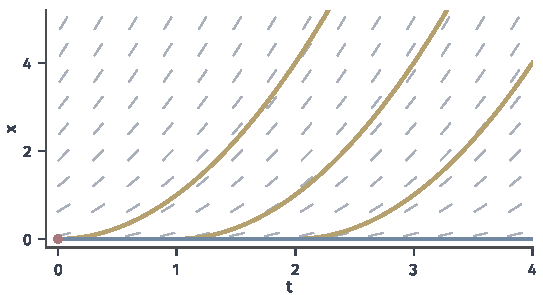
\includegraphics[width=92mm]{figures/06-differential-equations/01-ordinary-differential-equations/matplotlib/ivp-lost-solutions/figure.pdf}
 \caption{$\dot{x}=2\sqrt{\lvert x\rvert}$，$x(0)=0$的多个解。蓝线是平衡解$x\equiv 0$，黄线是式~\eqref{eq:ivp-sqrt-family}中$c=0,\,1,\,2$的解，它们在零解上停留一段时间后离开。}
 \label{fig:ivp-lost-solutions}
\end{BookInlineFigure}

图~\ref{fig:ivp-lost-solutions}显示，从同一个初值出发有无穷多条解。若先除以$\sqrt{x}$，就只会得到$x=t^2$这一条，把$x\equiv 0$和其余的解都丢掉了。所以分离变量的第一步是列出$b$的全部零点，分别处理；这个例子还说明，处理完零点也不代表解已经找全。什么条件能保证解唯一，是第~\ref{chap:ode-existence-continuation}章的主题。

\paragraph{时间等于路程除以速度}
解能否走到$b$的零点，能否走到无穷远，都可以从定理的公式读出来。取$a\equiv 1$，$B(x)=t-t_0$可以写成
\begin{equation}
 t-t_0=\int_{x_0}^{x(t)}\frac{\mathrm{d}\xi}{b(\xi)}.
 \label{eq:ivp-travel-time}
\end{equation}
这和“时间等于路程除以速度”是同一回事：$b(\xi)$是状态走到$\xi$处的速度，$1/b$是走单位路程的耗时，经过的时间就是$1/b$曲线下的面积。图~\ref{fig:ivp-slowness}展示了三种情形。

\begin{BookInlineFigure}
 \centering
 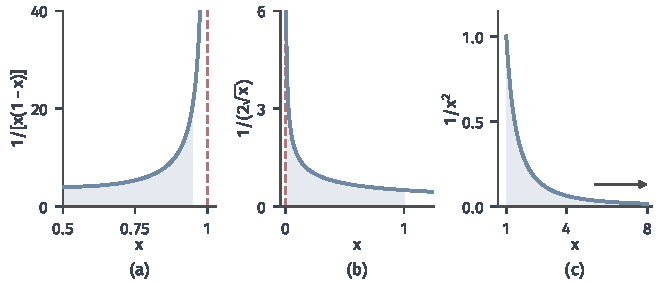
\includegraphics[width=112mm]{figures/06-differential-equations/01-ordinary-differential-equations/matplotlib/ivp-slowness/figure.pdf}
 \caption{经过时间等于$1/b$曲线下的面积。(a)$b=x(1-x)$：$1/b$在$x=1$处的积分发散，浅蓝区是从$0.5$到$0.95$所用的时间，走到$1$需要无穷长时间。(b)$b=2\sqrt{x}$：在$x=0$处的奇异可积，从$0$走到$1$只用时间$1$。(c)$b=x^2$：$1/x^2$在无穷远可积，从$1$走到无穷远只用时间$1$。}
 \label{fig:ivp-slowness}
\end{BookInlineFigure}

(a)中$b$在零点附近像线性函数，$1/b$像$1/\lvert x-1\rvert$，积分对数发散，解需要无穷长的时间才能接近平衡，这和$x_0=0.1$的解只是逐渐趋于$1$一致。(b)中$b$在零点附近比线性函数大得多，$1/b$可积，走到零点只需有限时间，于是解可以到达零点甚至从零点离开，这就是图~\ref{fig:ivp-lost-solutions}的现象。(c)中速度增长得足够快，$1/b$在无穷远可积，到达无穷远只需有限时间，这是爆炸的原因。

\subsection{变量代换}
\label{sec:ivp-substitution}

有些方程本身不可分离，换一个未知量后就可以分离或变成线性。代换$w=\psi(t,x)$的基本要求是：对每个$t$，$\psi(t,\cdot)$在所讨论的范围内可逆，并且连续可微且导数非零。否则新旧方程的解不再一一对应。每次代换都要回答三个问题：在什么范围内可逆，零点和被排除的点是否对应别的解，新未知量的取值范围是什么。

\paragraph{齐次型方程}
若右端只依赖比值$x/t$，
\begin{equation}
 \dot{x}=F\Bigl(\frac{x}{t}\Bigr),\qquad t\neq 0,
 \label{eq:ivp-homogeneous}
\end{equation}
则称方程为\term{齐次型方程}（homogeneous-type equation）。这个名称来自$F(x/t)$在缩放$(t,x)\mapsto(\lambda t,\lambda x)$下不变：同一条过原点的射线上，方向场的斜率相同，如图~\ref{fig:ivp-homogeneous-rays}(a)中的浅色射线所示。

既然比值$v=x/t$决定一切，就用它作新未知量。把$x=tv$代入，$\dot{x}=v+t\dot{v}$，于是
\begin{equation}
 \dot{v}=\frac{F(v)-v}{t}.
 \label{eq:ivp-homogeneous-reduced}
\end{equation}
这是可分离方程，$a(t)=1/t$，$b(v)=F(v)-v$。

\begin{lemma}[比例代换的可逆性]
 \label{lem:ivp-homogeneous}
 设$I$是不含$0$的区间，$F$在开区间$V$上连续。函数$x:I\to\mathbb{R}$可微、满足$x(t)/t\in V$且解式~\eqref{eq:ivp-homogeneous}，当且仅当$v(t)=x(t)/t$可微、取值于$V$且解式~\eqref{eq:ivp-homogeneous-reduced}。
\end{lemma}

\begin{proof}
 在$I$上$t\neq 0$，所以$x\mapsto x/t$和$v\mapsto tv$互为逆映射，两者保持可微性。由$x=tv$得$\dot{x}=v+t\dot{v}$。因此$\dot{x}=F(v)$等价于$v+t\dot{v}=F(v)$，再除以$t\neq 0$就得到式~\eqref{eq:ivp-homogeneous-reduced}。
\end{proof}

条件$t\neq 0$就是可逆性的范围。若所求区间含$0$，比值代换在$t=0$处失效，需要在$t>0$和$t<0$两侧分别讨论。零点方面，$F(v^{\star})=v^{\star}$给出$v\equiv v^{\star}$，对应的$x=v^{\star}t$是一条过原点的直线解，分离变量时要单独列出。

下面用一个例子走完全程：
\[
 \dot{x}=\frac{x}{t}+\frac{x^2}{t^2},\qquad x(1)=1,\qquad t>0.
\]
这里$F(v)=v+v^2$，$F(v)-v=v^2$，式~\eqref{eq:ivp-homogeneous-reduced}成为
\[
 \dot{v}=\frac{v^2}{t},\qquad v(1)=1.
\]
零点$v^{\star}=0$对应直线解$x\equiv 0$。初值$v(1)=1>0$，取$D_0=(0,\infty)$，由定理~\ref{thm:ivp-separation}，
\[
 B(v)=1-\frac{1}{v},\qquad A(t)=\ln t.
\]
令$B(v)=A(t)$，解出
\[
 v(t)=\frac{1}{1-\ln t}.
\]
值域$J=(-\infty,1)$要求$\ln t<1$，换回原变量得到
\begin{equation}
 x(t)=\frac{t}{1-\ln t},\qquad 0<t<\mathrm{e}.
 \label{eq:ivp-homogeneous-example}
\end{equation}

代回检验。由式~\eqref{eq:ivp-homogeneous-example}，比值$x/t=1/(1-\ln t)$，直接计算导数：
\[
 \dot{x}=\frac{(1-\ln t)+1}{(1-\ln t)^2}=\frac{1}{1-\ln t}+\frac{1}{(1-\ln t)^2}=\frac{x}{t}+\frac{x^2}{t^2}.
\]
并且$x(1)=1$。解在$t\uparrow\mathrm{e}$时爆炸。在$t\downarrow 0$时$x\to 0$，但右端在$t=0$无定义，解也到此为止。

\begin{BookInlineFigure}
 \centering
 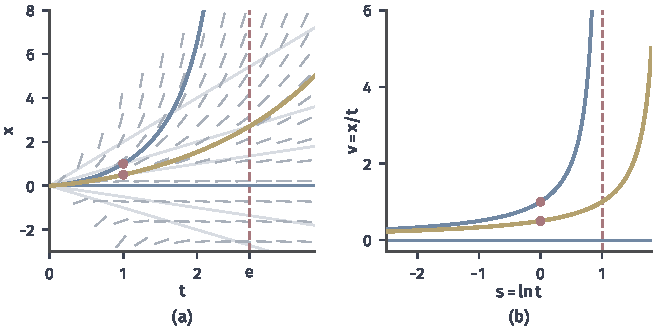
\includegraphics[width=112mm]{figures/06-differential-equations/01-ordinary-differential-equations/matplotlib/ivp-homogeneous-rays/figure.pdf}
 \caption{$\dot{x}=x/t+x^2/t^2$。(a)方向场在每条过原点的浅色射线上斜率相同。蓝线是$x(1)=1$的解$t/(1-\ln t)$，在$t=\mathrm{e}$（红色虚线）爆炸；黄线是$x(1)=0.5$的解$t/(2-\ln t)$；水平蓝线是$x\equiv 0$。(b)同样的解在坐标$s=\ln t$，$v=x/t$下满足自治方程$\mathrm{d}v/\mathrm{d}s=v^2$。}
 \label{fig:ivp-homogeneous-rays}
\end{BookInlineFigure}

图~\ref{fig:ivp-homogeneous-rays}(b)再做一次时钟变换$s=\ln t$，由式~\eqref{eq:ivp-homogeneous-reduced}得$\mathrm{d}v/\mathrm{d}s=v^2$。这正是第~\ref{sec:ivp-verification}节的爆炸方程，$v=1/(1-s)$。齐次型方程在缩放下的对称性，经过比值代换和对数时钟，变成了自治方程的时间平移不变性。

\paragraph{Bernoulli方程}
第二种代换把非线性项吸收掉。形如
\begin{equation}
 \dot{x}=p(t)\,x+q(t)\,x^{\alpha},\qquad\alpha\neq 0,\,1
 \label{eq:ivp-bernoulli}
\end{equation}
的方程称为\term{Bernoulli方程}（Bernoulli equation），$p$、$q$连续。$\alpha=0$或$1$时它本身就是线性的，所以排除这两种情况。

方程非线性，是因为$x^{\alpha}$与$x$次数不同。两边除以$x^{\alpha}$，得到$x^{-\alpha}\dot{x}=p\,x^{1-\alpha}+q$，左边恰好是$x^{1-\alpha}$导数的倍数。令
\begin{equation}
 w=x^{1-\alpha},
 \label{eq:ivp-bernoulli-substitution}
\end{equation}
则$\dot{w}=(1-\alpha)x^{-\alpha}\dot{x}$，代入得到线性方程
\begin{equation}
 \dot{w}=(1-\alpha)p(t)\,w+(1-\alpha)q(t).
 \label{eq:ivp-bernoulli-linear}
\end{equation}

\begin{lemma}[Bernoulli代换]
 \label{lem:ivp-bernoulli}
 在$x>0$的范围内，函数$x:I\to(0,\infty)$可微且解式~\eqref{eq:ivp-bernoulli}，当且仅当$w=x^{1-\alpha}:I\to(0,\infty)$可微且解式~\eqref{eq:ivp-bernoulli-linear}。
\end{lemma}

\begin{proof}
 因为$\alpha\neq 1$，$x\mapsto x^{1-\alpha}$是$(0,\infty)$到自身的连续可微双射，逆映射是$w\mapsto w^{1/(1-\alpha)}$，同样连续可微，所以两个方向都保持可微性。由链式法则，
 \[
 \dot{w}=(1-\alpha)x^{-\alpha}\dot{x}.
 \]
 把$\dot{x}$换成式~\eqref{eq:ivp-bernoulli}的右端，再用$x^{1-\alpha}=w$，就得到式~\eqref{eq:ivp-bernoulli-linear}。反方向把这一计算倒过来，用到$(1-\alpha)x^{-\alpha}\neq 0$。
\end{proof}

式~\eqref{eq:ivp-bernoulli-linear}系数依赖时间时，解法由第~\ref{chap:linear-differential-systems}章的积分因子给出。下面的例子系数为常数，可以用本节的方法完成。

Logistic方程$\dot{x}=x-x^2$是$p=1$，$q=-1$，$\alpha=2$的情形。代换$w=1/x$给出$\dot{w}=-w+1$。令$u=w-1$，$\dot{u}=-u$，所以$u=u_0\mathrm{e}^{-t}$，即
\[
 w(t)=1+(w_0-1)\mathrm{e}^{-t}.
\]
取$x_0=0.1$，$w_0=10$，$w=1+9\mathrm{e}^{-t}$，$x=1/w=\mathrm{e}^{t}/(\mathrm{e}^{t}+9)$，与式~\eqref{eq:ivp-logistic-solution}相同。图~\ref{fig:ivp-bernoulli-linearize}显示了这个代换的效果：$S$形的曲线变成了指数曲线。

\begin{BookInlineFigure}
 \centering
 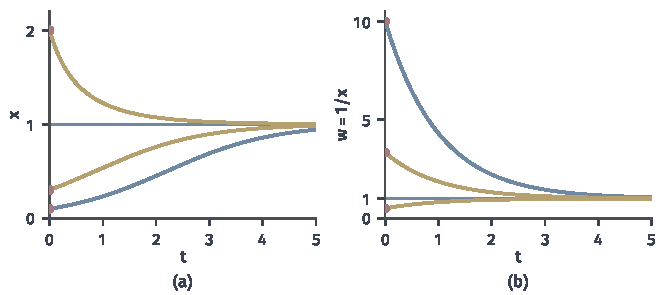
\includegraphics[width=112mm]{figures/06-differential-equations/01-ordinary-differential-equations/matplotlib/ivp-bernoulli-linearize/figure.pdf}
 \caption{代换$w=1/x$把Logistic方程变成线性方程。(a)$x_0=0.1$（蓝）与$x_0=0.3,\,2$（黄）的解。(b)同样三条解的$w=1/x=1+(w_0-1)\mathrm{e}^{-t}$，水平蓝线是$x\equiv 1$对应的$w\equiv 1$。平衡解$x\equiv 0$对应$w=\infty$，在(b)中没有位置。}
 \label{fig:ivp-bernoulli-linearize}
\end{BookInlineFigure}

这里的代换$w=1/x$对$x\neq 0$都可逆，所以负初值也能处理。$x_0=-0.5$时$w_0=-2$，$w=1-3\mathrm{e}^{-t}$，$w$在$t=\ln 3$处穿过零，对应$x\to-\infty$。原方程里的爆炸在$w$方程里只是平淡地穿过$0$，所以$w$的解可以继续，$x$的解却到此为止，这就是要核对取值范围的原因。而$x\equiv 0$对应$w=\infty$，代换把它排除在外，需要单独列出。

下一个例子演示符号的丢失。对$\dot{x}=x-x^3$，$\alpha=3$，代换$w=x^{-2}$给出$\dot{w}=-2w+2$，解是
\[
 w(t)=1+(w_0-1)\mathrm{e}^{-2t}.
\]
取$x_0=0.4$，$w_0=6.25$，$w=1+5.25\mathrm{e}^{-2t}$。若$x_0=-0.4$，$w_0$仍是$6.25$，得到完全相同的$w$。这时$w$只记录了$x$的大小，符号要从初值恢复：
\[
 x(t)=\operatorname{sign}(x_0)\,\bigl(1+5.25\mathrm{e}^{-2t}\bigr)^{-1/2}.
\]
由于$x\mapsto x^{-2}$在$\mathbb{R}\setminus\{0\}$上不是单射，代换只在$x>0$与$x<0$上分别可逆。解不能穿过$x=0$，否则$w$要经过无穷大。图~\ref{fig:ivp-bernoulli-sign}展示了这一点。

\begin{BookInlineFigure}
 \centering
 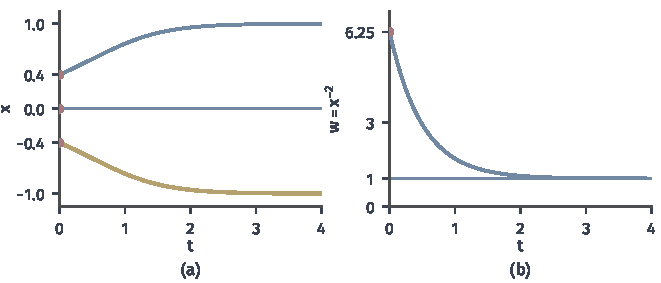
\includegraphics[width=112mm]{figures/06-differential-equations/01-ordinary-differential-equations/matplotlib/ivp-bernoulli-sign/figure.pdf}
 \caption{$\dot{x}=x-x^3$的代换$w=x^{-2}$。(a)初值$x_0=0.4$（蓝）与$x_0=-0.4$（黄）的解，以及平衡解$x\equiv 0$（红点是三个初值）。(b)$\pm 0.4$的解映成同一条$w=1+5.25\mathrm{e}^{-2t}$，水平蓝线对应$x\equiv\pm 1$。$x\equiv 0$在$w$中没有对应。}
 \label{fig:ivp-bernoulli-sign}
\end{BookInlineFigure}

最后看$\alpha<1$的情况，比如$\dot{x}=2\sqrt{x}$，$\alpha=1/2$，$p=0$，$q=2$。代换$w=\sqrt{x}$给出$\dot{w}=1$，线性方程的解唯一，$w=w_0+t$。可是上一小节已经看到，$x_0=0$时原方程有无穷多解。矛盾来自引理~\ref{lem:ivp-bernoulli}的范围：$x\mapsto\sqrt{x}$在$x=0$处不可微，等式$\dot{w}=\dot{x}/(2\sqrt{x})$在那里没有意义，解一旦碰到$x=0$，新旧方程就不再等价。形式上的化简可以很干净，它给出的却不一定是原问题的全部解。

下表整理这些代换的适用范围。
\begin{BookInlineTable}
 \centering
 \caption{变量代换的核验项}
 \label{tab:ivp-substitution}
 \begin{tabular}{llll}
 \toprule
 方程 & 代换 & 可逆范围 & 需单独检查 \\
 \midrule
 $\dot{x}=F(x/t)$ & $v=x/t$ & $t\neq 0$ & 直线解$x=v^{\star}t$ \\
 $\dot{x}=x-x^2$ & $w=1/x$ & $x\neq 0$ & $x\equiv 0$，$w$过零 \\
 $\dot{x}=x-x^3$ & $w=x^{-2}$ & $x>0$或$x<0$ & $x\equiv 0$，符号 \\
 $\dot{x}=2\sqrt{x}$ & $w=\sqrt{x}$ & $x>0$ & 碰到$x=0$的解 \\
 \bottomrule
 \end{tabular}
\end{BookInlineTable}

\section{积分形式}
\label{sec:ivp-integral}

解析解的方法到此为止，绝大多数方程不属于上面这些类型。没有公式时还能怎样谈论解？微分方程约束的是导数，而导数对曲线的小改动极其敏感。把方程两边从起点积分，导数就消失了，得到的新形式更容易分析。

\paragraph{累积变化}
设$\bm{x}$是解。状态在$[t_0,t]$上的变化，是沿途所有瞬时变化率的累积，而瞬时变化率就是方程的右端。于是
\begin{equation}
 \bm{x}(t)=\bm{x}_0+\int_{t_0}^{t}\bm{f}\bigl(s,\bm{x}(s)\bigr)\,\mathrm{d}s.
 \label{eq:ivp-integral}
\end{equation}
这里的积分对向量逐分量进行，$t<t_0$时按有向积分理解。式~\eqref{eq:ivp-integral}称为初值问题的\term{积分形式}（integral form）。

用Logistic方程的解检验这个读法。沿解$x=\mathrm{e}^{s}/(9+\mathrm{e}^{s})$的速度是$x(1-x)=9\mathrm{e}^{s}/(9+\mathrm{e}^{s})^2$，它的原函数是$-9/(9+\mathrm{e}^{s})$，所以从$0$累积到$\ln 9$的面积是
\[
 \int_0^{\ln 9}\frac{9\mathrm{e}^{s}}{(9+\mathrm{e}^{s})^2}\,\mathrm{d}s
 =-\frac{9}{18}+\frac{9}{10}=0.4.
\]
这正好等于$x(\ln 9)-x(0)=0.5-0.1$，如图~\ref{fig:ivp-integral-area}(a)(b)所示。

\begin{BookInlineFigure}
 \centering
 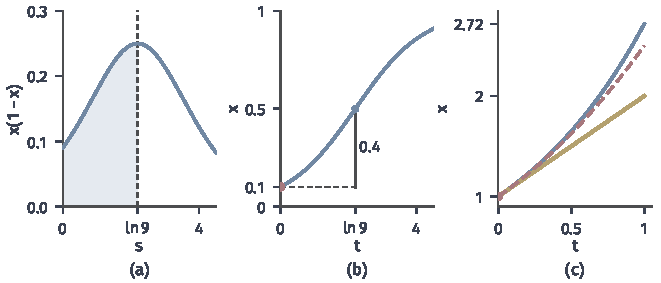
\includegraphics[width=112mm]{figures/06-differential-equations/01-ordinary-differential-equations/matplotlib/ivp-integral-area/figure.pdf}
 \caption{积分形式的读法。(a)沿Logistic解的速度曲线$x(1-x)$，浅蓝区是从$0$到$\ln 9$的累积，面积为$0.4$。(b)解曲线在同一段上的增量恰为$0.4$。(c)方程$\dot{x}=x$，$x(0)=1$：黄线是试探曲线$1+t$，红色虚线是把它代入式~\eqref{eq:ivp-integral}右端得到的$1+t+t^2/2$，蓝线是真解$\mathrm{e}^{t}$，只有真解代入后不变。}
 \label{fig:ivp-integral-area}
\end{BookInlineFigure}

\paragraph{两种形式等价}
微分形式要求曲线可微，积分形式只要求右端能积分。连续右端下，两者描述同样的曲线。

\begin{theorem}[微分形式与积分形式的等价性]
 \label{thm:ivp-integral-equivalence}
 设$\bm{f}$在$T\times\bm{D}$上连续，$I\subseteq T$是包含$t_0$的区间，$\bm{x}:I\to\bm{D}$连续。则$\bm{x}$是初值问题~\eqref{eq:ivp-ivp}在$I$上的经典解，当且仅当$\bm{x}$在$I$上处处满足积分方程~\eqref{eq:ivp-integral}。
\end{theorem}

\begin{proof}
 设$\bm{x}$是经典解。由第~\ref{sec:ivp-verification}节的说明，$\dot{\bm{x}}(s)=\bm{f}(s,\bm{x}(s))$连续。对每个分量用微积分基本定理，
 \[
 \bm{x}(t)-\bm{x}(t_0)=\int_{t_0}^{t}\dot{\bm{x}}(s)\,\mathrm{d}s
 =\int_{t_0}^{t}\bm{f}\bigl(s,\bm{x}(s)\bigr)\,\mathrm{d}s,
 \]
 再代入$\bm{x}(t_0)=\bm{x}_0$，就得到式~\eqref{eq:ivp-integral}。

 反过来，设连续曲线$\bm{x}$满足式~\eqref{eq:ivp-integral}。$\bm{f}$连续、$\bm{x}$连续，所以被积函数$s\mapsto\bm{f}(s,\bm{x}(s))$连续。由微积分基本定理的另一方向，式~\eqref{eq:ivp-integral}右端关于$t$连续可微，导数等于$\bm{f}(t,\bm{x}(t))$，这就是微分方程。令$t=t_0$，积分为零，得到初值。
\end{proof}

定理用到的是连续函数的微积分基本定理，可参考\BookChapterRef{chap:univariate-integration}{卷一第7章“一元函数的积分”}。证明里连续性出现了两次：$\bm{f}$连续让被积函数连续，从而让变上限积分可导。若$\bm{f}$在时间上有跳变，这一步就会失败，下一节处理这种情形。

\paragraph{积分形式保留了初值}
微分方程$\dot{\bm{x}}=\bm{f}(t,\bm{x})$本身不知道从哪里出发，初值要另外写。积分方程把初值写在了式子里：$\bm{x}_0$就是右端的第一项，令$t=t_0$立刻读出。例如在$\dot{x}=\cos t$中，$\sin t$和$\sin t+5$是同一个微分方程的两条解，而积分方程$x(t)=x_0+\int_0^t\cos s\,\mathrm{d}s$对给定的$x_0$只有一条解。

\paragraph{解是自洽的曲线}
式~\eqref{eq:ivp-integral}还有一个结构上的特点：未知曲线同时出现在两边。曲线决定沿途的速度，速度累积后必须重新给出同一条曲线。若把右端看作把一条曲线变成另一条曲线的映射，解就是这个映射的不动点。

拿方程$\dot{x}=x$，$x(0)=1$来试。积分方程是$x(t)=1+\int_0^t x(s)\,\mathrm{d}s$。把试探曲线$x(t)=1+t$代入右端，得到
\[
 1+\int_0^t(1+s)\,\mathrm{d}s=1+t+\frac{t^2}{2},
\]
与试探曲线不同，所以$1+t$不是解。把$\mathrm{e}^{t}$代入，右端是$1+(\mathrm{e}^{t}-1)=\mathrm{e}^{t}$，映射后不变。图~\ref{fig:ivp-integral-area}(c)比较了这三条曲线。解的存在性和唯一性由第~\ref{chap:ode-existence-continuation}章从这个不动点结构出发证明，那里的Picard迭代正是反复做这种代入。

\paragraph{积分比导数温和}
积分形式好用的另一个原因，是积分对小扰动不敏感，而导数恰好相反。取
\[
 \delta(t)=\varepsilon\sin\frac{t}{\varepsilon^2},
\]
$\varepsilon$很小时，这是一个幅度为$\varepsilon$的高频抖动。它的导数和变上限积分分别是
\[
 \dot{\delta}(t)=\frac{1}{\varepsilon}\cos\frac{t}{\varepsilon^2},\qquad
 \int_0^t\delta(s)\,\mathrm{d}s=\varepsilon^3\Bigl(1-\cos\frac{t}{\varepsilon^2}\Bigr).
\]
曲线本身的差距是$\varepsilon$，导数的差距却有$1/\varepsilon$，积分的差距只有$2\varepsilon^3$。图~\ref{fig:ivp-integral-smoothing}取$\varepsilon=0.2$，三个幅度是$0.2$、$5$和$0.016$。

\begin{BookInlineFigure}
 \centering
 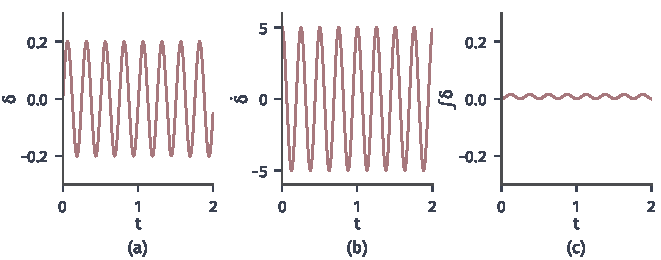
\includegraphics[width=112mm]{figures/06-differential-equations/01-ordinary-differential-equations/matplotlib/ivp-integral-smoothing/figure.pdf}
 \caption{高频小扰动$\delta(t)=\varepsilon\sin(t/\varepsilon^2)$，$\varepsilon=0.2$。(a)扰动本身，幅度$0.2$。(b)导数，幅度$5$。(c)变上限积分，幅度不超过$2\varepsilon^3=0.016$，(a)和(c)使用相同的纵轴。}
 \label{fig:ivp-integral-smoothing}
\end{BookInlineFigure}

这个对比说明了两种形式的不同用处。两条曲线接近时，它们的导数可能相差很大，所以在微分形式中无法比较；积分形式中，两边都只涉及曲线本身的值。设$\bm{x}$、$\tilde{\bm{x}}$分别是初值$\bm{x}_0$、$\tilde{\bm{x}}_0$对应的解，相减得到
\begin{equation}
 \bm{x}(t)-\tilde{\bm{x}}(t)=\bm{x}_0-\tilde{\bm{x}}_0+\int_{t_0}^{t}\bigl[\bm{f}(s,\bm{x}(s))-\bm{f}(s,\tilde{\bm{x}}(s))\bigr]\,\mathrm{d}s,
 \label{eq:ivp-integral-difference}
\end{equation}
差值完全由差值控制，不出现导数。第~\ref{chap:ode-sensitivity}章从这个等式出发估计数据误差的影响。

\paragraph{解的光滑性}
积分形式也回答了解有多光滑。若$\bm{f}$连续，由定理~\ref{thm:ivp-integral-equivalence}，$\bm{x}$连续可微。若$\bm{f}$进一步是$k$次连续可微的，可以一阶一阶往上推。假设已知$\bm{x}$是$j$次连续可微的，$j\leq k$，则复合函数$s\mapsto\bm{f}(s,\bm{x}(s))$也是$j$次连续可微的，而$\bm{x}$是它的变上限积分加常数，所以$\bm{x}$是$j+1$次连续可微的。从$j=1$推到$j=k$，得到$\bm{x}$是$k+1$次连续可微的：解总比右端多一阶光滑。Logistic方程的右端是多项式，所以解是无穷次可微的。

下表归纳两种形式的不同之处。
\begin{BookInlineTable}
 \centering
 \caption{微分形式与积分形式}
 \label{tab:ivp-two-forms}
 \begin{tabular}{lll}
 \toprule
 比较项 & 微分形式 & 积分形式 \\
 \midrule
 对曲线的要求 & 可微 & 被积函数可积 \\
 初值 & 另外给出 & 写在式子里 \\
 对小扰动 & 导数可以很大 & 积分很小 \\
 适合做什么 & 代入检验 & 证明与误差估计 \\
 \bottomrule
 \end{tabular}
\end{BookInlineTable}

\section{可测输入}
\label{sec:ivp-measurable}

前面的结论都假设右端连续。实际的输入常常不连续：开关切换，继电器动作，信号被采样后保持。这时曲线在切换时刻不可能处处满足方程，解又该怎样定义？积分形式给出答案。

\paragraph{一次切换}
一个房间的温度偏差$x$满足$\dot{x}=-x+g(t)$，$x(0)=0$，暖气的作用是
\[
 g(t)=\begin{cases}1,&0\leq t<1,\\0,&t\geq 1.\end{cases}
\]
在$[0,1)$上$g\equiv 1$，这是冷却方程~\eqref{eq:ivp-cooling}的情形（$k=1$，$c=1$），由式~\eqref{eq:ivp-cooling-solution}，
\[
 x(t)=1-\mathrm{e}^{-t},\qquad 0\leq t\leq 1.
\]
温度不会突变，所以第二段以$x(1)=1-\mathrm{e}^{-1}\approx 0.632$为初值。在$t\geq 1$上$\dot{x}=-x$，因此
\[
 x(t)=(1-\mathrm{e}^{-1})\,\mathrm{e}^{-(t-1)},\qquad t\geq 1.
\]

\begin{BookInlineFigure}
 \centering
 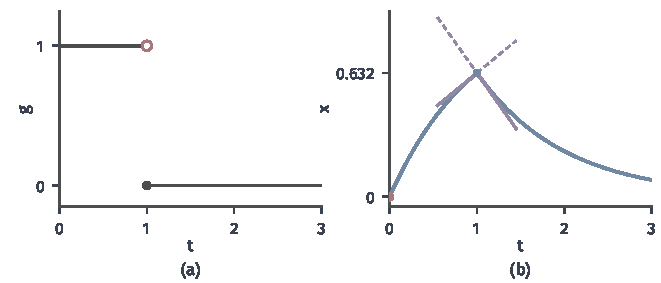
\includegraphics[width=112mm]{figures/06-differential-equations/01-ordinary-differential-equations/matplotlib/ivp-switching-input/figure.pdf}
 \caption{一次切换。(a)输入$g$在$t=1$从$1$跳到$0$。(b)解在$t=1$处连续但有折角。紫色实线是左右两侧的切线，斜率分别为$\mathrm{e}^{-1}\approx 0.368$和$-0.632$，紫色虚线是它们的延长。}
 \label{fig:ivp-switching-input}
\end{BookInlineFigure}

图~\ref{fig:ivp-switching-input}(b)的曲线在$t=1$连续，但左右导数不同：
\[
 \dot{x}(1^{-})=-0.632+1=0.368,\qquad\dot{x}(1^{+})=-0.632.
\]
这样的曲线在$t=1$不可微，不是定义~\ref{def:ivp-classical-solution}意义下的解，并且无论把$g(1)$规定成什么都不可能是。把两段分别解出来再接起来，所得的曲线却是唯一合理的答案。它的一个重要性质是满足积分方程：对$t\leq 1$，
\[
 \int_0^t(-x(s)+1)\,\mathrm{d}s=\int_0^t\mathrm{e}^{-s}\,\mathrm{d}s=1-\mathrm{e}^{-t}=x(t).
\]
对$t>1$，把积分在$1$处分开，后一段被积函数是$-x(s)$，由此验证
\[
 x(1)+\int_1^t(-x(s))\,\mathrm{d}s
 =x(1)+x(1)\bigl(\mathrm{e}^{-(t-1)}-1\bigr)=x(t).
\]
积分不在乎被积函数在一个点上的取值，所以$g(1)$取$0$或$1$都不影响。这启发我们用积分方程作为解的定义。

\paragraph{切换无穷多次}
有限次切换总可以分段解决。但输入可能更不规则。图~\ref{fig:ivp-irregular-inputs}给出两种情形，方程都取$\dot{x}=g(t)$，$x(0)=0$，所以解就是$g$的累积。

第一种，$g(t)=\operatorname{sign}\sin(1/t)$，$t\in(0,1]$。切换点$1/(k\pi)$在$t=0$附近聚集，无法从起点开始分段：不存在“第一段”。

第二种，$g$是胖Cantor集$C\subset[0,1]$的指示函数。构造方法是：第$k$步从剩下的每段中间挖去长度$4^{-k}$的开区间，极限集合$C$是闭集，不含任何区间，总长度却是$1-\sum_{k\geq 1}2^{k-1}4^{-k}=1/2$。$g$在$C$的每一点都不连续，而这些点的总长度为正，所以$g$不是Riemann可积的，分段的办法和连续函数的积分都不适用。

\begin{BookInlineFigure}
 \centering
 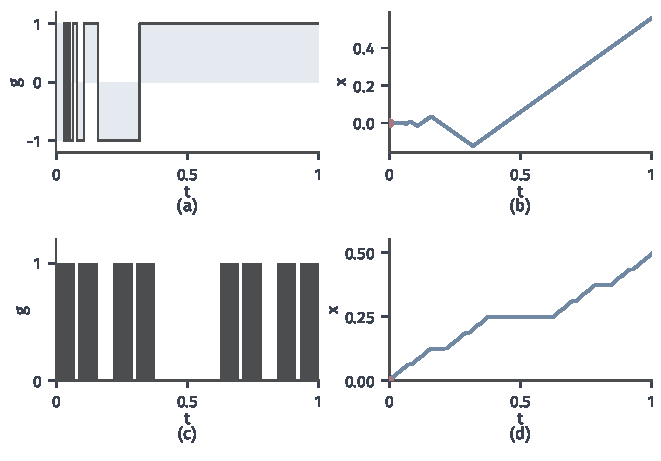
\includegraphics[width=112mm]{figures/06-differential-equations/01-ordinary-differential-equations/matplotlib/ivp-irregular-inputs/figure.pdf}
 \caption{不能分段处理的输入，方程为$\dot{x}=g$，$x(0)=0$。(a)$g=\operatorname{sign}\sin(1/t)$，切换点向$t=0$聚集（$t<0.03$只画出浅色填充）。(b)它的累积。(c)胖Cantor集的指示函数（挖到第$11$层的近似）。(d)它的累积$x(t)$是$[0,t]$中集合$C$的长度，$x(1)=1/2$。}
 \label{fig:ivp-irregular-inputs}
\end{BookInlineFigure}

两种情形中$g$都是有界可测函数，Lebesgue积分有意义，累积$x(t)=\int_0^t g$是连续曲线。这两条累积曲线都不能分成有限段来求，却也都由输入唯一确定，解的概念应当能容纳它们。

\paragraph{为什么要绝对连续}
一个自然的想法是放宽为“连续，并且几乎处处满足方程”。这不够。考虑$\dot{x}=0$，$x(0)=0$，Cantor函数$c:[0,1]\to[0,1]$满足$c(0)=0$，它连续，在Cantor集之外导数为零，而Cantor集长度为零，所以它几乎处处满足方程。可是$c(1)=1$，它一路上升了，而方程说的是不变。图~\ref{fig:ivp-cantor-candidate}中的红线就是这样的假解。

\begin{BookInlineFigure}
 \centering
 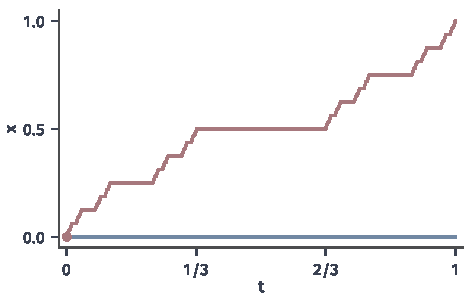
\includegraphics[width=80mm]{figures/06-differential-equations/01-ordinary-differential-equations/matplotlib/ivp-cantor-candidate/figure.pdf}
 \caption{方程$\dot{x}=0$，$x(0)=0$的解是蓝线$x\equiv 0$。红线是Cantor函数，连续且几乎处处导数为零，却从$0$升到$1$，不满足积分方程$x(t)=0+\int_0^t0\,\mathrm{d}s$。}
 \label{fig:ivp-cantor-candidate}
\end{BookInlineFigure}

Cantor函数的全部增长都发生在一个长度为零的集合上，导数看不见它，所以累积不回去。我们需要的正是“增量可以由导数累积回来”的函数，这恰是绝对连续函数的特征。区间$[a,b]$上的函数$F$称为\term{绝对连续函数}，是指对任意$\varepsilon>0$，存在$\delta>0$，使总长度小于$\delta$的有限个不交子区间上的增量绝对值之和小于$\varepsilon$。

这个定义恰好对应一种形式的微积分基本定理：$F$绝对连续，当且仅当存在可积函数$v$，使$F(t)=F(a)+\int_a^tv$；此时$F$几乎处处可导，并且$\dot{F}=v$几乎处处成立。这一结论及Cantor函数不绝对连续的证明，可参考\BookChapterRef{chap:integration}{卷四第6章“积分”}。向量值曲线的绝对连续按分量理解。若曲线在区间$I$的每个有限闭子区间上绝对连续，就称它局部绝对连续。

\paragraph{绝对连续解}
有了这个概念，就可以给出解的定义。

\begin{definition}[绝对连续解]
 \label{def:ivp-ac-solution}
 设$\bm{f}:T\times\bm{D}\to\mathbb{R}^{n}$，$t_0\in T$，$\bm{x}_0\in\bm{D}$，$I\subseteq T$是包含$t_0$的非退化区间。曲线$\bm{x}:I\to\bm{D}$称为初值问题的\term{绝对连续解}（absolutely continuous solution，也称Carathéodory解），若$\bm{x}$局部绝对连续，$\bm{x}(t_0)=\bm{x}_0$，并且
 \begin{equation}
 \dot{\bm{x}}(t)=\bm{f}\bigl(t,\bm{x}(t)\bigr)\quad\text{对几乎每个}t\in I\text{成立。}
 \label{eq:ivp-ac-solution}
 \end{equation}
\end{definition}

“几乎每个”的意思是，方程不成立的时刻构成一个Lebesgue测度为零的集合。图~\ref{fig:ivp-switching-input}的曲线只在$t=1$这一点不满足方程，是绝对连续解。图~\ref{fig:ivp-irregular-inputs}的累积也都是绝对连续解。

\begin{lemma}[积分形式的刻画]
 \label{lem:ivp-ac-integral}
 设$\bm{x}:I\to\bm{D}$连续，且$s\mapsto\bm{f}(s,\bm{x}(s))$在$I$上局部可积。则$\bm{x}$是绝对连续解，当且仅当它处处满足积分方程~\eqref{eq:ivp-integral}。反过来，任何绝对连续解都使$s\mapsto\bm{f}(s,\bm{x}(s))$局部可积。
\end{lemma}

\begin{proof}
 先证最后一句。若$\bm{x}$是绝对连续解，$\dot{\bm{x}}$局部可积，而$\bm{f}(s,\bm{x}(s))$与它几乎处处相等。Lebesgue测度是完备的，零测集上的改动不影响可测性，所以这个函数也局部可积。

 设$\bm{x}$是绝对连续解。对$t\in I$，在$t_0$与$t$之间的闭区间上用绝对连续函数的基本定理：
 \[
 \bm{x}(t)-\bm{x}(t_0)=\int_{t_0}^{t}\dot{\bm{x}}(s)\,\mathrm{d}s
 =\int_{t_0}^{t}\bm{f}\bigl(s,\bm{x}(s)\bigr)\,\mathrm{d}s,
 \]
 第二个等号用到被积函数几乎处处相等。代入初值，就是式~\eqref{eq:ivp-integral}。

 反过来，设$\bm{x}$满足式~\eqref{eq:ivp-integral}。局部可积函数的变上限积分局部绝对连续，并且几乎处处可导，导数几乎处处等于被积函数。这正是式~\eqref{eq:ivp-ac-solution}。令$t=t_0$得到初值。
\end{proof}

连续右端的情形被包含在内。若$\bm{f}$连续，$\bm{x}$是绝对连续解，则$s\mapsto\bm{f}(s,\bm{x}(s))$连续，由引理~\ref{lem:ivp-ac-integral}和定理~\ref{thm:ivp-integral-equivalence}，$\bm{x}$是经典解。所以绝对连续解是推广，不是另一套标准：右端连续时，两者是同一个东西。

\paragraph{什么样的输入可以用}
引理的前提是被积函数局部可积，它取决于输入。对式~\eqref{eq:ivp-input-system}，设$\bm{h}$连续，输入$\bm{g}$可测且在每个有限闭区间上有界（可以除去零测集）。对任何连续曲线$\bm{x}$，映射$s\mapsto(\bm{x}(s),\bm{g}(s))$可测，与连续函数$\bm{h}$的复合也可测。在有限闭区间上，$\bm{x}$的值域是紧集，$\bm{g}$几乎处处落在一个有界集内，于是$\bm{h}$的取值有界，被积函数可积。

这正是图~\ref{fig:ivp-irregular-inputs}两种输入的情形。输入有界并不是必需的，但完全不加控制也不行。对比两个在$t=0$无界的输入，方程都是$\dot{x}=g(t)$，$x(0)=0$，如图~\ref{fig:ivp-integrable-singular}所示。

$g(t)=t^{-1/2}$在$[0,1]$上可积，累积是$x(t)=2\sqrt{t}$。这条曲线绝对连续，在$t=0$处右导数无穷大，但方程只需要几乎处处成立，它是解。

$g(t)=1/t$在$0$附近不可积。从$t=1$往回算，累积是$\ln t$，当$t\downarrow 0$时趋于$-\infty$。不存在从$x(0)=0$出发的有限曲线，积分方程在这里没有意义。

\begin{BookInlineFigure}
 \centering
 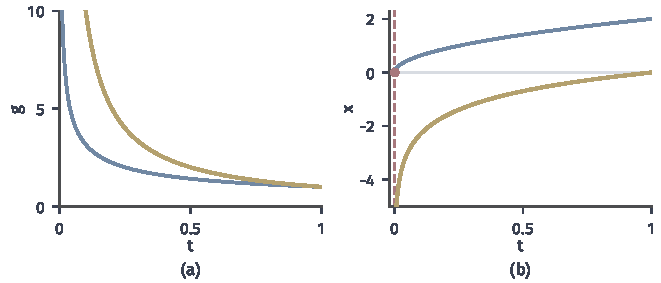
\includegraphics[width=112mm]{figures/06-differential-equations/01-ordinary-differential-equations/matplotlib/ivp-integrable-singular/figure.pdf}
 \caption{$t=0$处无界的输入。(a)$g=t^{-1/2}$（蓝）可积，$g=1/t$（黄）不可积。(b)蓝线是$\dot{x}=t^{-1/2}$，$x(0)=0$的解$2\sqrt{t}$；黄线是$\ln t$，当$t\downarrow 0$时发散，无法接到$t=0$（红色虚线）。}
 \label{fig:ivp-integrable-singular}
\end{BookInlineFigure}

这里只是检验给定曲线是否是解，并没有断言解一定存在。要保证存在，还需要右端对时间可测、对状态连续，并且在状态的紧集上被一个时间的可积函数控制；唯一性还需要状态方向上的局部Lipschitz系数对时间局部可积。这些条件和结论由第~\ref{chap:ode-existence-continuation}章给出。

\paragraph{时间方向与状态方向的不对称}
上面的不连续都在时间方向上。解穿过一个时间点只花一瞬间，那一点上右端的值不影响积分，所以时间方向的跳变是无害的。状态方向的跳变不同，解可能在跳变处长期停留，这时零测集的论证就失效了。

考虑$\dot{x}=-\sigma(x)$，$x(0)=0$，其中$\sigma(x)=1$（$x\geq 0$），$\sigma(x)=-1$（$x<0$）。这个方程在任何区间$[0,\varepsilon)$上都没有绝对连续解。

假设有解。若某时刻$t_1>0$有$x(t_1)>0$，取$t_2$为$t_1$之前$x$最后一次等于$0$的时刻。在$(t_2,t_1]$上$x>0$，方程给出$\dot{x}=-1$几乎处处成立，积分得$x(t_1)=-(t_1-t_2)<0$，矛盾。

若$x(t_1)<0$，同样取$t_2$，在$(t_2,t_1]$上$\dot{x}=+1$，积分得$x(t_1)=t_1-t_2>0$，也矛盾。所以$x\equiv 0$。但这时$\dot{x}=0$，而方程要求$\dot{x}=-\sigma(0)=-1$几乎处处成立，仍然矛盾。

这个反例说明，第~\ref{sec:ivp-state}节的扩充状态不能随便用来处理不连续的输入。把时间写成状态分量$s$之后，右端对$s$是不连续的，表面上成了“状态方向的跳变”。但因为$\dot{s}=1$，解以单位速度穿过$s$的每一个值，并不停留，所以这种不连续恰好无害。一般的状态方向的不连续不具备这个性质。假设中对时间只要求可测、对状态要求连续，分工的依据就在这里。

\paragraph{解的概念的层次}
图~\ref{fig:ivp-solution-classes}整理了本章出现的曲线类。越往外，允许的曲线越多，能用的输入越一般。绝对连续这一层的外面，曲线已经无法由导数累积回来，所以解的概念止步于此。

\begin{BookInlineFigure}
 \centering
 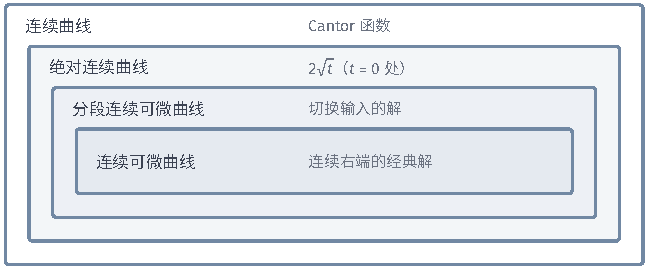
\includegraphics[width=109mm]{figures/06-differential-equations/01-ordinary-differential-equations/tikz/ivp-solution-classes/figure.pdf}
 \caption{本章涉及的曲线类，外层包含内层，右侧是每层的代表例子。连续右端的解在最内层，切换输入的解在第二层，可测输入的解在绝对连续这一层。Cantor函数只是连续，不能作为解。}
 \label{fig:ivp-solution-classes}
\end{BookInlineFigure}

\section{本章小结}
\label{sec:ivp-summary}

本章从规律和起点出发，确定了初值问题的提法。一个初值问题由右端$\bm{f}$、初始时刻$t_0$和初值$\bm{x}_0$组成，答案是一条曲线及其存在区间，两者都要回答。相同的规律从不同的初值出发是不同的曲线，这是方向场所显示的基本事实。初值集中在一个时刻，因此可以沿时间往前推；两点边值的条件分在两头，同样的方程可能无解或有无穷多解。

状态是此刻足以决定下一瞬间变化的量。高阶方程把直到$m-1$阶的导数放进状态，降为一阶系统；单摆需要角度和角速度。时间、状态、外部输入和参数各有角色。右端不显含时间的方程称为自治方程，它的解可以平移；非自治方程可以通过把时间并入状态写成自治方程，代价是增加一维，并把时间上的不正则转移到状态分量上。

解的概念决定了什么才算求解。经典解要在一个区间上处处可微、满足方程和初值，这个要求排除了隐式公式的错误分支，也说明了存在区间可能因定义域的边界或有限时间爆炸而有限。平衡解容易在除法中丢掉，需要单独列出。

解析方法只对具体形式的方程有效。可分离方程由$B(x)=A(t)$得到解，$B$的值域决定存在区间，$b$的零点需要分别处理，$1/b$的可积性决定解能否到达零点或无穷远。齐次型方程和Bernoulli方程用代换化为可分离方程或线性方程，每次代换都要核对可逆范围、零点和取值范围，形式上干净的结果不一定是原问题的全部解。

积分形式把方程写成初值加累积，在连续右端下与微分形式等价。它自带初值，解是自洽的曲线，积分对小扰动不敏感。这个形式让我们能够处理时间方向不连续的可测输入：解的概念放宽为局部绝对连续的曲线，方程几乎处处成立，等价于积分方程处处成立。下表对比了两种解。

\begin{BookInlineTable}
 \centering
 \caption{经典解与绝对连续解}
 \label{tab:ivp-solution-comparison}
 \begin{tabular}{lll}
 \toprule
 & 经典解 & 绝对连续解 \\
 \midrule
 右端 & 连续 & 对时间可测 \\
 曲线 & 连续可微 & 局部绝对连续 \\
 方程 & 处处成立 & 几乎处处成立 \\
 积分方程 & 处处成立 & 处处成立 \\
 例子 & Logistic解 & 切换输入的解 \\
 \bottomrule
 \end{tabular}
\end{BookInlineTable}

没有公式时，仍然要回答解是否存在、是否唯一、能延伸多远，这是第~\ref{chap:ode-existence-continuation}章的任务；解对初值和参数有多敏感，由第~\ref{chap:ode-sensitivity}章估计；怎样算出解的数值，由第~\ref{chap:ode-numerical-methods}章讨论。线性方程可以写出完整的传播公式，是第~\ref{chap:linear-differential-systems}章的内容。


\chapter{线性微分方程}
\label{chap:linear-differential-systems}

一杯水放在温度恒定的房间里，同时有一台功率随时间变化的小加热器。水温相对室温的偏差$x(t)$按比例散失，又被加热器抬高，于是
\[
 \dot{x}=-kx+g(t).
\]
未知函数只以一次的形式出现。这个看似平常的特点带来一条很强的结论：把初始偏差加倍，初始偏差造成的那部分响应也加倍；两台加热器同时工作，响应等于各自单独工作时的响应之和。

一般的线性问题也是这样：一个初始状态和一段外部输入进入方程，得到一条响应曲线，而这个对应关系是线性的。本章围绕一个问题展开：怎样把这个线性对应关系明确算出来？

路线由简到繁。第~\ref{sec:lde-first-order}节用乘积求导解出标量方程。第~\ref{sec:lde-constant}节把指数函数推广到矩阵，处理常系数向量系统和高阶方程，解释指数、振荡和多项式因子从哪里来。第~\ref{sec:lde-time-varying}节去掉常系数的假设，建立任意两个时刻之间的传播，并说明为什么一般不能对系数矩阵积分后再取指数。

第~\ref{sec:lde-inhomogeneous}节加入输入，第~\ref{sec:lde-green}节把输入响应拆成一次次脉冲的叠加，第~\ref{sec:lde-laplace}节则用积分变换把常系数方程化成代数方程。矩阵的特征分解、Schur形和Jordan块沿用卷二的结果，用到时就地说明。

\section{一阶线性方程}
\label{sec:lde-first-order}

最简单的线性方程只有一个未知函数和一阶导数。设$I$是一个区间，$a,g:I\to\mathbb{R}$是给定函数，考虑
\begin{equation}
 \dot{x}(t)=a(t)x(t)+g(t),\qquad x(t_0)=x_0,\qquad t_0\in I.
 \label{eq:lde-scalar}
\end{equation}
称它为\term{一阶线性方程}（first-order linear equation）。系数$a(t)$说明当前状态怎样影响自身的变化，$g(t)$是外部输入。$g\equiv0$时方程称为\term{齐次线性方程}（homogeneous linear equation），否则称为非齐次线性方程。

\paragraph{叠加}
线性的含义可以直接验证。若$x_1$满足$\dot{x}_1=ax_1+g_1$，$x_2$满足$\dot{x}_2=ax_2+g_2$，则对常数$c_1,c_2$，组合$c_1x_1+c_2x_2$满足同一个方程，输入变为$c_1g_1+c_2g_2$。这就是\term{叠加原理}（superposition principle）。

特别地，同一输入下两个解的差满足齐次方程。所以只要找到一个解，其他解都等于它加上某个齐次解。下面的工作因此分成两件事：求齐次解，求一个带输入的解。

\paragraph{从乘积求导到积分因子}
方程~\eqref{eq:lde-scalar}的困难在于$\dot{x}-ax$不是任何函数的导数，无法直接积分。乘积求导公式却提供了一种可能。对一个待定的正函数$\mu(t)$，有
\[
 \frac{\mathrm{d}}{\mathrm{d}t}\bigl(\mu x\bigr)=\mu\dot{x}+\dot{\mu}x.
\]
把方程改写成$\dot{x}-ax=g$，两边乘$\mu$，左边是$\mu\dot{x}-a\mu x$。只要它恰好是上面的乘积导数，就要求
\[
 \dot{\mu}=-a\mu.
\]

这是一个不含$x$的齐次方程，它的一个正解是
\begin{equation}
 \mu(t)=\exp\Bigl(-\int_{t_0}^{t}a(r)\,\mathrm{d}r\Bigr).
 \label{eq:lde-integrating-factor}
\end{equation}
这个$\mu$称为\term{积分因子}（integrating factor），选取下限$t_0$使$\mu(t_0)=1$。乘上它之后，方程变成
\[
 \frac{\mathrm{d}}{\mathrm{d}t}\bigl(\mu(t)x(t)\bigr)=\mu(t)g(t).
\]

右端不再含未知函数，从$t_0$积分到$t$，并利用$\mu(t_0)=1$，得到
\[
 \mu(t)x(t)-x_0=\int_{t_0}^{t}\mu(s)g(s)\,\mathrm{d}s.
\]
两边除以$\mu(t)$就解出了$x(t)$。比值$\mu(s)/\mu(t)$恰好等于从$s$到$t$累积系数的指数，记
\begin{equation}
 \Phi(t,s)=\frac{\mu(s)}{\mu(t)}=\exp\Bigl(\int_{s}^{t}a(r)\,\mathrm{d}r\Bigr).
 \label{eq:lde-scalar-propagator}
\end{equation}
$\Phi(t,s)$把时刻$s$的齐次状态传播到时刻$t$，第~\ref{sec:lde-time-varying}节会建立它的矩阵版本。

\begin{theorem}[连续系数的一阶线性方程]
\label{thm:lde-scalar-solution}
设$a,g$在区间$I$上连续，$t_0\in I$，$x_0\in\mathbb{R}$。则初值问题~\eqref{eq:lde-scalar}在整个$I$上有唯一的连续可微解，它是
\begin{equation}
 x(t)=\Phi(t,t_0)x_0+\int_{t_0}^{t}\Phi(t,s)g(s)\,\mathrm{d}s.
 \label{eq:lde-scalar-solution}
\end{equation}
\end{theorem}

\begin{proof}
先证唯一。设$x$是$I$上的连续可微解，上面的推导每一步都合法：$\mu$连续可微且恒正，乘积求导成立，$\mu g$连续，可以用微积分基本定理积分。所以$x$必须等于式~\eqref{eq:lde-scalar-solution}。

再证这个公式确实给出解。由式~\eqref{eq:lde-scalar-propagator}，它可以写成
\[
 x(t)=\frac{1}{\mu(t)}\Bigl(x_0+\int_{t_0}^{t}\mu(s)g(s)\,\mathrm{d}s\Bigr).
\]
由$\dot{\mu}=-a\mu$得$(1/\mu)^{\cdot}=a/\mu$。对乘积求导，第一项得$a(t)x(t)$，第二项由积分上限求导得$g(t)$，所以
\[
 \dot{x}(t)=a(t)x(t)+g(t).
\]
代入$t=t_0$，积分为零，$\Phi(t_0,t_0)=1$，得$x(t_0)=x_0$。
\end{proof}

公式~\eqref{eq:lde-scalar-solution}的两项有清楚的含义。第一项是初值独自传播的结果。第二项把每一时刻的输入$g(s)\,\mathrm{d}s$看成一笔小的状态增量，它从时刻$s$起按$\Phi(t,s)$传播到$t$，再全部累加。

连续性条件的作用也很具体：它保证$\mu$可微，保证$\mu g$能用微积分基本定理积分。结论中的存在区间是整个$I$，这与非线性方程不同。第~\ref{chap:ordinary-differential-equations}章的$\dot{x}=x^2$、$x(0)=1$有解$1/(1-t)$，在$t=1$爆炸；线性方程右端关于$x$只按一次增长，公式~\eqref{eq:lde-scalar-solution}在系数有定义的地方都有意义。

\begin{example}[正弦输入的散热]
\label{ex:lde-sine-input}
求解$\dot{x}=-x+\sin t$，$x(0)=x_0$。这里$a=-1$，所以$\Phi(t,s)=\mathrm{e}^{-(t-s)}$。由式~\eqref{eq:lde-scalar-solution}，
\[
 x(t)=\mathrm{e}^{-t}x_0+\mathrm{e}^{-t}\int_0^t\mathrm{e}^{s}\sin s\,\mathrm{d}s.
\]
分部积分两次可得$\mathrm{e}^{s}(\sin s-\cos s)/2$是$\mathrm{e}^{s}\sin s$的一个原函数，于是
\[
 \int_0^t\mathrm{e}^{s}\sin s\,\mathrm{d}s=\frac{\mathrm{e}^{t}(\sin t-\cos t)+1}{2}.
\]
代回并合并$\mathrm{e}^{-t}$的项，得到
\[
 x(t)=\Bigl(x_0+\frac12\Bigr)\mathrm{e}^{-t}+\frac{\sin t-\cos t}{2}.
\]
令$x_{\mathrm{p}}(t)=(\sin t-\cos t)/2$，它是$x_0=-1/2$对应的特解。对它求导，
\[
 \dot{x}_{\mathrm{p}}=\frac{\cos t+\sin t}{2}=-x_{\mathrm{p}}+\sin t,
\]
所以$x_{\mathrm{p}}$确实满足方程。常数$x_0+1/2$由初值唯一确定。
\end{example}

图~\ref{fig:lde-first-order-family}把这个分解画了出来。方向场的短线段是每点的斜率，解曲线沿短线段前进。不同初值的解之差是$(x_0-x_0')\mathrm{e}^{-t}$，它们在几个时间单位内贴到同一条黄色曲线上。

\begin{BookInlineFigure}
  \centering
  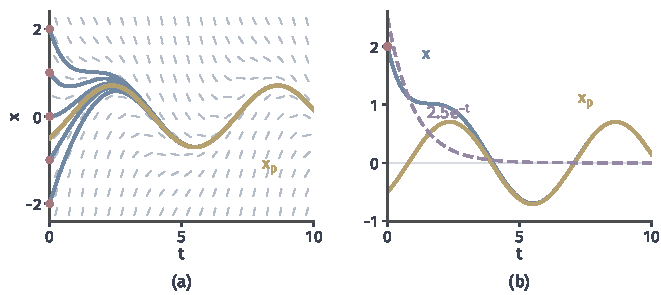
\includegraphics[width=112mm]{figures/06-differential-equations/01-ordinary-differential-equations/matplotlib/lde-first-order-family/figure.pdf}
  \caption{方程$\dot{x}=-x+\sin t$的解族与分解。(a)灰色短线是方向场，蓝线是初值$x_0=-2,-1,0,1,2$（红点）的解，黄线是特解$x_{\mathrm{p}}$。(b)$x_0=2$的解（蓝）等于紫色虚线$2.5\mathrm{e}^{-t}$与黄色特解之和。}
  \label{fig:lde-first-order-family}
\end{BookInlineFigure}

\paragraph{积分因子做了什么}
再看一个系数随时间变化的例子，$\dot{x}=-2tx+2t$，$x(0)=x_0$。这里$\int_0^t a=-t^2$，积分因子是$\mu(t)=\mathrm{e}^{t^2}$。令$y=\mu x$，方程变成
\[
 \dot{y}=2t\mathrm{e}^{t^2}.
\]
右端不再依赖状态，积分得到$y(t)=x_0+\mathrm{e}^{t^2}-1$。除以$\mu$，结果是
\[
 x(t)=1+(x_0-1)\mathrm{e}^{-t^2}.
\]

图~\ref{fig:lde-integrating-factor}对比了$x$和$y$两个坐标。原坐标中的解曲线互相靠拢，斜率同时依赖$t$和$x$。换成$y=\mu x$以后，同一时刻各点斜率相同，解曲线彼此只差一个上下平移，积分因此可以直接进行。

可以把$\mu(t)$想成一把随时间伸缩的尺子。齐次部分造成的伸缩被这把尺子抵消，剩下的只有输入的累积。这个类比只对线性方程成立：非线性方程中伸缩率依赖状态本身，不同解需要不同的尺子。

\begin{BookInlineFigure}
  \centering
  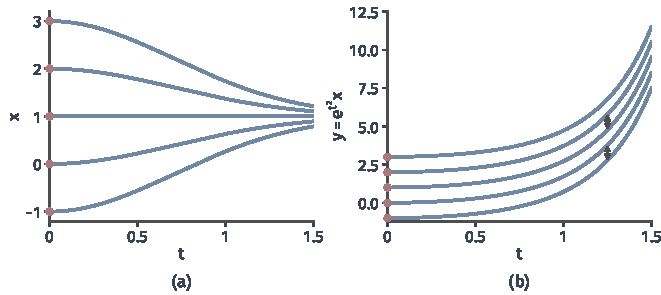
\includegraphics[width=112mm]{figures/06-differential-equations/01-ordinary-differential-equations/matplotlib/lde-integrating-factor/figure.pdf}
  \caption{积分因子的作用，方程$\dot{x}=-2tx+2t$，红点是初值$x_0=-1,0,1,2,3$。(a)原坐标中的解。(b)变量$y=\mathrm{e}^{t^2}x$下，同一批解彼此只差上下平移，黑色双箭头示意相邻两条曲线在同一时刻的间距都是$1$。}
  \label{fig:lde-integrating-factor}
\end{BookInlineFigure}

\paragraph{解的区间由系数决定}
定理~\ref{thm:lde-scalar-solution}要求系数在$I$上连续，$I$之外不作任何保证。考虑$\dot{x}=-x/t+1$，$x(1)=x_0$。系数$a(t)=-1/t$在$t=0$没有定义，初值点$t_0=1$所在的最大连续区间是$I=(0,\infty)$。

由式~\eqref{eq:lde-scalar-propagator}，$\Phi(t,s)=\exp(-\ln t+\ln s)=s/t$。代入式~\eqref{eq:lde-scalar-solution}，
\[
 x(t)=\frac{x_0}{t}+\int_1^t\frac{s}{t}\,\mathrm{d}s=\frac{x_0}{t}+\frac{t^2-1}{2t}.
\]
令$c=x_0-1/2$，解化成
\[
 x(t)=\frac{c}{t}+\frac{t}{2},\qquad t\in(0,\infty).
\]

图~\ref{fig:lde-singular-coefficient}中，$c\neq0$的解在$t\to0^+$时无界，$c=0$的解$x=t/2$却可以一直延伸到$t=0$。这里的奇异位置$t=0$由系数决定，所有解都在同一处遇到它；而$\dot{x}=x^2$的爆炸时刻随初值变化。线性方程的解走不出系数的连续区间，也只有在这个边界上才可能失控。

\begin{BookInlineFigure}
  \centering
  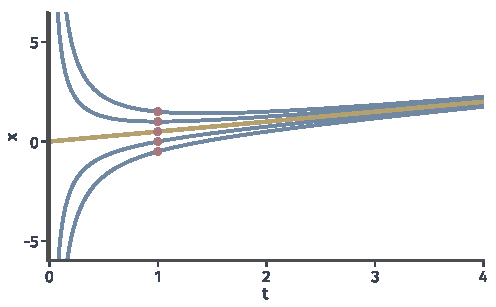
\includegraphics[width=84mm]{figures/06-differential-equations/01-ordinary-differential-equations/matplotlib/lde-singular-coefficient/figure.pdf}
  \caption{系数决定解的区间。方程$\dot{x}=-x/t+1$的解$x=c/t+t/2$，红点是$t=1$处的初值，蓝线取$c=\pm1,\pm0.5$，黄线取$c=0$。左侧深灰粗线$t=0$处系数$-1/t$无定义，所有$c\neq0$的解都在此无界。}
  \label{fig:lde-singular-coefficient}
\end{BookInlineFigure}

\paragraph{可积系数}
第~\ref{chap:ordinary-differential-equations}章说明过，系数或输入只是可测时，解未必处处可微，要用积分形式理解。对线性方程，这种解的含义是：$x$在$I$的每个紧子区间上绝对连续，在$I$上几乎处处满足微分方程，并且$x(t_0)=x_0$。与之等价的写法是
\begin{equation}
 x(t)=x_0+\int_{t_0}^{t}\bigl(a(s)x(s)+g(s)\bigr)\,\mathrm{d}s,\qquad t\in I.
 \label{eq:lde-scalar-integral}
\end{equation}
绝对连续函数的导数几乎处处存在且可积，并能积分回原函数，可参考\BookChapterRef{chap:integration}{卷四第6章“积分”}。

\begin{theorem}[可积系数的一阶线性方程]
\label{thm:lde-scalar-integrable}
设$a,g$在$I$的每个紧子区间上Lebesgue可积，$t_0\in I$。则式~\eqref{eq:lde-scalar-solution}定义的函数是积分方程~\eqref{eq:lde-scalar-integral}在$I$上的唯一局部绝对连续解。
\end{theorem}

\begin{proof}
此时$b(t)=\int_{t_0}^ta$局部绝对连续，$\mu=\mathrm{e}^{-b}$是绝对连续函数与光滑函数的复合，在紧子区间上$b$有界，所以$\mu$与$1/\mu$都局部绝对连续，并且几乎处处有$\dot{\mu}=-a\mu$。

先证唯一。设$x$是局部绝对连续解。局部绝对连续函数的乘积仍局部绝对连续，所以$\mu x$局部绝对连续，几乎处处有
\[
 (\mu x)^{\cdot}=\mu(\dot{x}-ax)=\mu g.
\]
$\mu$在紧子区间上有界，$\mu g$可积。对绝对连续函数用微积分基本定理，得$\mu(t)x(t)-x_0=\int_{t_0}^t\mu g$，这正是式~\eqref{eq:lde-scalar-solution}。

再证存在。令$y(t)=x_0+\int_{t_0}^t\mu g$，它局部绝对连续，几乎处处$\dot{y}=\mu g$。令$x=y/\mu$，它局部绝对连续，并且几乎处处
\[
 \dot{x}=\frac{a}{\mu}y+\frac{1}{\mu}\mu g=ax+g.
\]
再积分回去就得到式~\eqref{eq:lde-scalar-integral}。
\end{proof}

公式没有变化，变化的只是它的解释：求导只在几乎处处成立，真正对每一点都成立的是积分形式。图~\ref{fig:lde-integrable-coefficient}给出两种典型情况。

\begin{example}[两种不光滑的系数]
\label{ex:lde-integrable-coefficients}
第一种是系数跳变。取$x(0)=1$，$g=0$，$a(t)=-1$（$0\leq t<1$），$a(t)=-3$（$t\geq1$）。计算$\int_0^t a$，得到
\[
 x(t)=\begin{cases}\mathrm{e}^{-t},&0\leq t\leq1,\\ \mathrm{e}^{-1}\mathrm{e}^{-3(t-1)},&t\geq1.\end{cases}
\]
左导数$-\mathrm{e}^{-1}$与右导数$-3\mathrm{e}^{-1}$在$t=1$不同，解在这一点不可微，其余各点都满足方程。

第二种是系数在端点无界但可积。取$a(t)=-1/(2\sqrt{t})$，$x(0)=1$。由$\int_0^ta=-\sqrt{t}$得
\[
 x(t)=\mathrm{e}^{-\sqrt{t}}.
\]
它在$t>0$满足方程，导数$-\mathrm{e}^{-\sqrt{t}}/(2\sqrt{t})$在$t\to0^+$时趋于$-\infty$。$x$在$t=0$不可微，式~\eqref{eq:lde-scalar-integral}仍然成立。
\end{example}

\begin{BookInlineFigure}
  \centering
  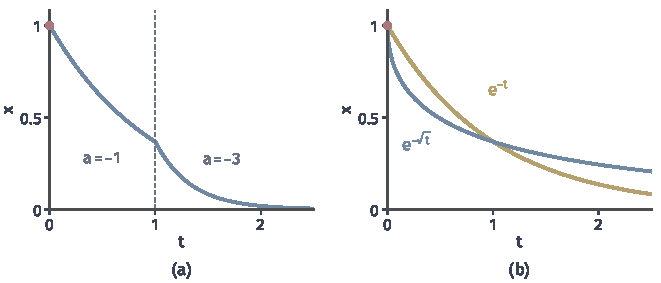
\includegraphics[width=112mm]{figures/06-differential-equations/01-ordinary-differential-equations/matplotlib/lde-integrable-coefficient/figure.pdf}
  \caption{可积系数下的绝对连续解，红点是初值$x(0)=1$。(a)系数在$t=1$从$-1$跳到$-3$，解连续但有折角。(b)系数$-1/(2\sqrt{t})$在$0$处无界但可积，解$\mathrm{e}^{-\sqrt{t}}$（蓝）在$0$处切线竖直；黄线$\mathrm{e}^{-t}$作对照，它在$0$处斜率有限。}
  \label{fig:lde-integrable-coefficient}
\end{BookInlineFigure}


\section{常系数方程}
\label{sec:lde-constant}

一个未知函数不够用时，状态就成了向量。设$\bm{A}\in\mathbb{R}^{n\times n}$是常数矩阵，考虑
\begin{equation}
 \dot{\bm{x}}(t)=\bm{A}\bm{x}(t),\qquad \bm{x}(t_0)=\bm{x}_0.
 \label{eq:lde-constant-system}
\end{equation}
标量情形的解是$\mathrm{e}^{(t-t_0)a}x_0$。向量情形需要回答：矩阵的“指数”是什么，它为什么能解方程，又怎样算出来？高阶标量方程随后会放进同一框架。

\subsection{矩阵指数解}
\label{sec:lde-matrix-exponential}

指数函数的幂级数只用到加法、数乘和乘幂，这些运算对方阵都有定义。于是把级数中的数$a$换成矩阵$\bm{A}$。

\begin{definition}[矩阵指数]
\label{def:lde-matrix-exponential}
对$\bm{A}\in\mathbb{R}^{n\times n}$和$t\in\mathbb{R}$，定义\term{矩阵指数}（matrix exponential）
\begin{equation}
 \mathrm{e}^{t\bm{A}}=\sum_{k=0}^{\infty}\frac{t^k\bm{A}^k}{k!}=\bm{I}+t\bm{A}+\frac{t^2\bm{A}^2}{2}+\cdots.
 \label{eq:lde-matrix-exponential}
\end{equation}
\end{definition}

下面的性质逐条对应标量指数的性质，只有第4条多了一个可交换的条件。

\begin{theorem}[矩阵指数的基本性质]
\label{thm:lde-matexp-properties}
设$\bm{A},\bm{B}\in\mathbb{R}^{n\times n}$，$s,t\in\mathbb{R}$。
\begin{enumerate}
 \item 级数~\eqref{eq:lde-matrix-exponential}绝对收敛，在$t$的有界集上一致收敛，并且
 \begin{equation}
  \lVert\mathrm{e}^{t\bm{A}}\rVert_2\leq\mathrm{e}^{\lvert t\rvert\lVert\bm{A}\rVert_2}.
  \label{eq:lde-matexp-bound}
 \end{equation}
 \item $\mathrm{e}^{0\bm{A}}=\bm{I}$，并且
 \begin{equation}
  \frac{\mathrm{d}}{\mathrm{d}t}\mathrm{e}^{t\bm{A}}=\bm{A}\mathrm{e}^{t\bm{A}}=\mathrm{e}^{t\bm{A}}\bm{A}.
  \label{eq:lde-matexp-derivative}
 \end{equation}
 \item 指数律成立，特别地，$\mathrm{e}^{t\bm{A}}$可逆，逆矩阵是$\mathrm{e}^{-t\bm{A}}$：
 \begin{equation}
  \mathrm{e}^{(t+s)\bm{A}}=\mathrm{e}^{t\bm{A}}\mathrm{e}^{s\bm{A}}.
  \label{eq:lde-matexp-group}
 \end{equation}
 \item 若$\bm{A}\bm{B}=\bm{B}\bm{A}$，则
 \begin{equation}
  \mathrm{e}^{t(\bm{A}+\bm{B})}=\mathrm{e}^{t\bm{A}}\mathrm{e}^{t\bm{B}}.
  \label{eq:lde-matexp-commuting}
 \end{equation}
 \item 若$\bm{V}$可逆，则
 \begin{equation}
  \mathrm{e}^{t\bm{V}\bm{B}\bm{V}^{-1}}=\bm{V}\mathrm{e}^{t\bm{B}}\bm{V}^{-1}.
  \label{eq:lde-matexp-similarity}
 \end{equation}
\end{enumerate}
\end{theorem}

\begin{proof}
(1)谱范数满足$\lVert\bm{A}^k\rVert_2\leq\lVert\bm{A}\rVert_2^k$，所以第$k$项的范数不超过$(\lvert t\rvert\lVert\bm{A}\rVert_2)^k/k!$。当$\lvert t\rvert\leq T$时，它被收敛的数值级数$\sum_k(T\lVert\bm{A}\rVert_2)^k/k!$的通项控制，一致收敛由优级数判别法得到。对这个不等式求和就是所述范数界。

(2)$t=0$时只剩首项$\bm{I}$。逐项求导得到
\[
 \sum_{k\geq1}\frac{t^{k-1}\bm{A}^k}{(k-1)!}=\bm{A}\sum_{j\geq0}\frac{t^{j}\bm{A}^{j}}{j!}.
\]
由(1)，导数级数在有界集上一致收敛，所以逐项求导合法。矩阵$\bm{A}$可以提到左边，也可以提到右边，因为它与自身的乘幂可交换。

(3)固定$s$，定义
\[
 \bm{Y}(t)=\mathrm{e}^{-t\bm{A}}\mathrm{e}^{(t+s)\bm{A}}.
\]
由(2)，
\[
 \dot{\bm{Y}}(t)=-\mathrm{e}^{-t\bm{A}}\bm{A}\mathrm{e}^{(t+s)\bm{A}}+\mathrm{e}^{-t\bm{A}}\bm{A}\mathrm{e}^{(t+s)\bm{A}}=\bm{0}.
\]
所以$\bm{Y}(t)=\bm{Y}(0)=\mathrm{e}^{s\bm{A}}$。取$s=0$得$\mathrm{e}^{-t\bm{A}}\mathrm{e}^{t\bm{A}}=\bm{I}$，方阵的左逆即逆。再用这个逆乘$\bm{Y}(t)=\mathrm{e}^{s\bm{A}}$的两边，就得到加法公式。

(4)$\bm{B}$与$\bm{A}$的每个乘幂可交换，所以$\bm{B}$与$\mathrm{e}^{t\bm{A}}$可交换。定义
\[
 \bm{Y}(t)=\mathrm{e}^{-t(\bm{A}+\bm{B})}\mathrm{e}^{t\bm{A}}\mathrm{e}^{t\bm{B}}.
\]
乘积求导得三项：
\[
 \dot{\bm{Y}}=\mathrm{e}^{-t(\bm{A}+\bm{B})}\bigl(-(\bm{A}+\bm{B})\mathrm{e}^{t\bm{A}}+\bm{A}\mathrm{e}^{t\bm{A}}+\mathrm{e}^{t\bm{A}}\bm{B}\bigr)\mathrm{e}^{t\bm{B}}.
\]
括号内由交换关系等于零，$\bm{Y}(t)=\bm{Y}(0)=\bm{I}$。再用(3)的逆矩阵乘回去。

(5)乘幂满足下式，其中相邻的$\bm{V}^{-1}\bm{V}$都消去了：
\[
 (\bm{V}\bm{B}\bm{V}^{-1})^k=\bm{V}\bm{B}^k\bm{V}^{-1}.
\]
代入级数，提出$\bm{V}$和$\bm{V}^{-1}$。
\end{proof}

\begin{theorem}[常系数齐次系统的解]
\label{thm:lde-constant-solution}
对任意$\bm{x}_0\in\mathbb{R}^n$，初值问题~\eqref{eq:lde-constant-system}在$\mathbb{R}$上有唯一解，它是
\begin{equation}
 \bm{x}(t)=\mathrm{e}^{(t-t_0)\bm{A}}\bm{x}_0.
 \label{eq:lde-constant-solution}
\end{equation}
\end{theorem}

\begin{proof}
由定理~\ref{thm:lde-matexp-properties}的(2)，式~\eqref{eq:lde-constant-solution}满足方程，$t=t_0$时等于$\bm{x}_0$。

反过来设$\bm{x}$是任意一个解，令$\bm{z}(t)=\mathrm{e}^{-(t-t_0)\bm{A}}\bm{x}(t)$。求导得
\[
 \dot{\bm{z}}=\mathrm{e}^{-(t-t_0)\bm{A}}(-\bm{A}\bm{x}+\dot{\bm{x}})=\bm{0}.
\]
所以$\bm{z}(t)=\bm{z}(t_0)=\bm{x}_0$，再乘$\mathrm{e}^{(t-t_0)\bm{A}}$就得到式~\eqref{eq:lde-constant-solution}。
\end{proof}

这个证明与积分因子完全平行：$\mathrm{e}^{-(t-t_0)\bm{A}}$扮演积分因子的角色，它和$\bm{A}$可交换，所以能够抵消方程右端。第~\ref{sec:lde-time-varying}节会看到，时变系数之所以困难，正是因为这种交换关系消失了。

先用级数算一个例子。取
\[
 \bm{J}_0=\begin{bmatrix}0&1\\-1&0\end{bmatrix},
\]
方程是$\dot{x}_1=x_2$、$\dot{x}_2=-x_1$。计算$\bm{J}_0^2=-\bm{I}$，级数的偶次项和奇次项分别凑成余弦和正弦：
\[
 \mathrm{e}^{t\bm{J}_0}=(\cos t)\bm{I}+(\sin t)\bm{J}_0=\begin{bmatrix}\cos t&\sin t\\-\sin t&\cos t\end{bmatrix}.
\]
矩阵的指数在这里是顺时针旋转。图~\ref{fig:lde-matexp-series}(a)画出从$(1,0)^{\top}$出发的轨道和截断到第$K$项的部分和。$K$越大，部分和贴住单位圆的时间越长。

图(b)是固定时刻的截断误差。余项首项的大小约为$t^{K+1}/(K+1)!$，$K$小于$t$时这一项还在增大，超过$t$之后才因阶乘而迅速下降，所以$t$越大需要的项数越多。

\begin{BookInlineFigure}
  \centering
  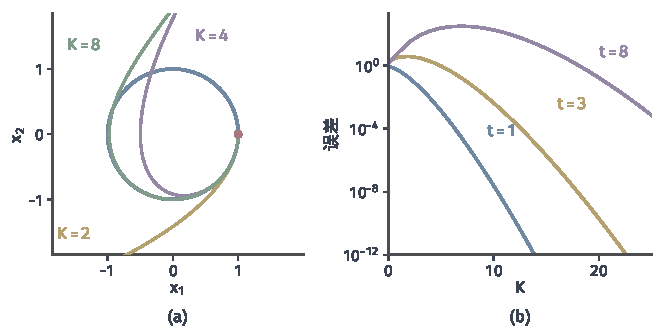
\includegraphics[width=112mm]{figures/06-differential-equations/01-ordinary-differential-equations/matplotlib/lde-matexp-series/figure.pdf}
  \caption{旋转矩阵$\bm{J}_0$的指数级数。(a)蓝色单位圆是精确轨道$\mathrm{e}^{t\bm{J}_0}(1,0)^{\top}$，彩色曲线是$t\in[0,1.5\pi]$上截断到第$K$项的部分和。(b)部分和与$\mathrm{e}^{t\bm{J}_0}$之差的谱范数，纵轴为对数，取$t=1,3,8$。}
  \label{fig:lde-matexp-series}
\end{BookInlineFigure}

\paragraph{对角化：解耦成独立的模式}
级数说明了矩阵指数是什么，计算时却要依靠矩阵的结构。若$\bm{A}$有$n$个线性无关的特征向量，就有$\bm{A}=\bm{V}\bm{\Lambda}\bm{V}^{-1}$，其中$\bm{V}$的列是特征向量$\bm{v}_i$，$\bm{\Lambda}$是特征值组成的对角阵。令$\bm{y}=\bm{V}^{-1}\bm{x}$，方程解耦成$n$个互不相干的标量方程：
\[
 \dot{y}_i=\lambda_iy_i,\qquad i=1,\ldots,n.
\]

记$\bm{w}_i^{\top}$为$\bm{V}^{-1}$的第$i$行。由定理~\ref{thm:lde-matexp-properties}的(5)和对角阵的指数，
\begin{equation}
 \mathrm{e}^{t\bm{A}}=\bm{V}\mathrm{e}^{t\bm{\Lambda}}\bm{V}^{-1}=\sum_{i=1}^{n}\mathrm{e}^{\lambda_it}\bm{v}_i\bm{w}_i^{\top}.
 \label{eq:lde-spectral-exponential}
\end{equation}
读法是：$\bm{w}_i^{\top}\bm{x}_0$量出初值在第$i$个特征方向上的分量，这个分量沿自己的方向按$\mathrm{e}^{\lambda_it}$变化。对角化以及下面用到的三角化（Schur形）的条件与计算，可参考\BookChapterRef{chap:eigen-spectral-decomposition}{卷二第6章“谱分解”}。

\begin{example}[贯穿全章的二维系统]
\label{ex:lde-running-system}
取
\[
 \bm{A}=\begin{bmatrix}0&1\\-2&-3\end{bmatrix}.
\]
特征多项式是$z^2+3z+2=(z+1)(z+2)$，特征值为$-1$和$-2$。解$(\bm{A}-\lambda\bm{I})\bm{v}=\bm{0}$，得到特征向量和它们组成的矩阵：
\[
 \bm{V}=\begin{bmatrix}1&1\\-1&-2\end{bmatrix},\qquad \bm{V}^{-1}=\begin{bmatrix}2&1\\-1&-1\end{bmatrix}.
\]
所以$\bm{w}_1^{\top}=(2,1)$，$\bm{w}_2^{\top}=(-1,-1)$。代入式~\eqref{eq:lde-spectral-exponential}，
\[
 \mathrm{e}^{t\bm{A}}=\mathrm{e}^{-t}\begin{bmatrix}2&1\\-2&-1\end{bmatrix}+\mathrm{e}^{-2t}\begin{bmatrix}-1&-1\\2&2\end{bmatrix}.
\]
取$t=0$，两个矩阵相加恰为$\bm{I}$，这是一次检验。取$\bm{x}_0=(1,0)^{\top}$，第一列给出
\[
 x_1(t)=2\mathrm{e}^{-t}-\mathrm{e}^{-2t},\qquad x_2(t)=-2\mathrm{e}^{-t}+2\mathrm{e}^{-2t}.
\]
再检验方程：$\dot{x}_1=-2\mathrm{e}^{-t}+2\mathrm{e}^{-2t}=x_2$，$\dot{x}_2=2\mathrm{e}^{-t}-4\mathrm{e}^{-2t}$，而
\[
 -2x_1-3x_2=2\mathrm{e}^{-t}-4\mathrm{e}^{-2t}.
\]
\end{example}

图~\ref{fig:lde-diagonal-modes}把同一批初值放在两个坐标系中。(a)的轨线弯曲，看不出规律；(b)用特征坐标后，两个坐标各自按$\mathrm{e}^{-t}$和$\mathrm{e}^{-2t}$收缩。$y_2$衰减得更快，所以轨线在到达原点前几乎都贴向$y_1$轴，在原坐标中表现为贴向$\bm{v}_1$方向。

\begin{BookInlineFigure}
  \centering
  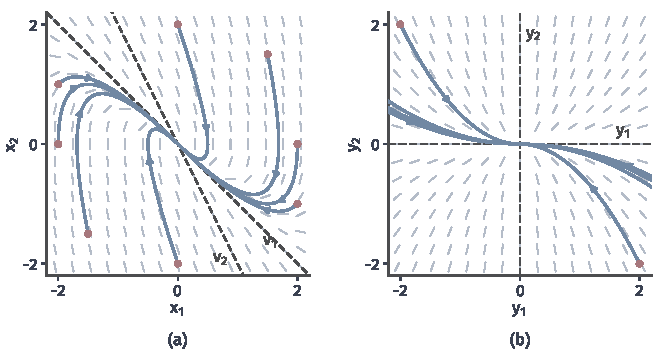
\includegraphics[width=112mm]{figures/06-differential-equations/01-ordinary-differential-equations/matplotlib/lde-diagonal-modes/figure.pdf}
  \caption{对角化解耦，系统取例~\ref{ex:lde-running-system}的$\bm{A}$。(a)原坐标的相平面，灰色短线是方向，蓝线是解，红点是初值，深灰虚线是特征方向$\bm{v}_1,\bm{v}_2$。(b)特征坐标$\bm{y}=\bm{V}^{-1}\bm{x}$中同一批解（超出显示范围的初值点未标出），特征方向成为坐标轴。}
  \label{fig:lde-diagonal-modes}
\end{BookInlineFigure}

\paragraph{复特征值：旋转与伸缩}
实矩阵可能有共轭复特征值$\alpha\pm\mathrm{i}\beta$（$\beta\neq0$）。式~\eqref{eq:lde-spectral-exponential}在复数域上仍然成立，但实系统的解是实的，更好的写法是看典型的二维块
\[
 \bm{A}=\begin{bmatrix}\alpha&\beta\\-\beta&\alpha\end{bmatrix}=\alpha\bm{I}+\beta\bm{J}_0.
\]
$\alpha\bm{I}$与任何矩阵可交换，由定理~\ref{thm:lde-matexp-properties}的(4)，
\begin{equation}
 \mathrm{e}^{t\bm{A}}=\mathrm{e}^{\alpha t}\begin{bmatrix}\cos\beta t&\sin\beta t\\-\sin\beta t&\cos\beta t\end{bmatrix}.
 \label{eq:lde-complex-block}
\end{equation}
实部$\alpha$负责伸缩，虚部$\beta$负责旋转的快慢。图~\ref{fig:lde-spiral}取$\alpha=-1$、$\beta=2$：相平面上是向内的螺线，分量则是被$\pm\mathrm{e}^{-t}$夹住的振荡。一般实矩阵的共轭特征值对，可以用实的相似变换化成这种二维块。

\begin{BookInlineFigure}
  \centering
  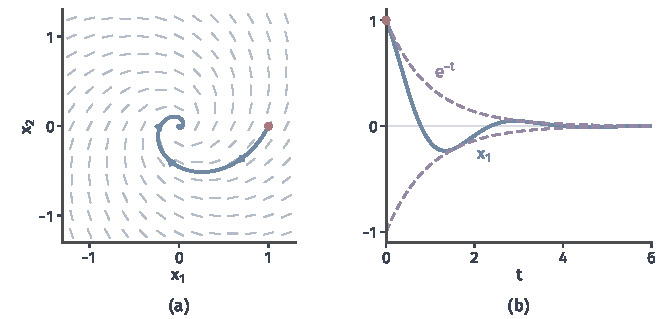
\includegraphics[width=112mm]{figures/06-differential-equations/01-ordinary-differential-equations/matplotlib/lde-spiral/figure.pdf}
  \caption{复特征值对应旋转与伸缩，$\bm{A}=\left[\begin{smallmatrix}-1&2\\-2&-1\end{smallmatrix}\right]$，特征值$-1\pm2\mathrm{i}$，初值$(1,0)^{\top}$（红点）。(a)相平面的螺线。(b)分量$x_1=\mathrm{e}^{-t}\cos2t$（蓝）与紫色虚线包络$\pm\mathrm{e}^{-t}$。}
  \label{fig:lde-spiral}
\end{BookInlineFigure}

\paragraph{三角形式：逐行回代}
不能对角化时，总可以退到三角形式。任意复方阵都酉相似于上三角阵$\bm{T}$，对角元是全部特征值；定理~\ref{thm:lde-matexp-properties}对复矩阵同样成立，证明不变。上三角系统的最后一行不含其他分量，可以先解出；倒数第二行以它为输入，又是一个一阶线性方程。于是第~\ref{sec:lde-first-order}节的公式可以逐行使用。

看一个具体的矩阵：
\[
 \bm{A}=\begin{bmatrix}-1&1\\0&-2\end{bmatrix}.
\]
第二行给出$x_2(t)=\mathrm{e}^{-2t}x_2(0)$。第一行是$\dot{x}_1=-x_1+x_2$，由式~\eqref{eq:lde-scalar-solution}，
\[
 x_1(t)=\mathrm{e}^{-t}x_1(0)+\Bigl(\int_0^t\mathrm{e}^{-(t-s)}\mathrm{e}^{-2s}\,\mathrm{d}s\Bigr)x_2(0).
\]
括号内的积分提出$\mathrm{e}^{-t}$后等于
\[
 \mathrm{e}^{-t}\int_0^t\mathrm{e}^{-s}\,\mathrm{d}s=\mathrm{e}^{-t}-\mathrm{e}^{-2t},
\]
所以
\[
 x_1(t)=\mathrm{e}^{-t}x_1(0)+(\mathrm{e}^{-t}-\mathrm{e}^{-2t})x_2(0).
\]

现在把第二个对角元也改成$-1$。积分变成$\int_0^t\mathrm{e}^{-(t-s)}\mathrm{e}^{-s}\,\mathrm{d}s$，被积函数恒等于$\mathrm{e}^{-t}$，与$s$无关，积分结果是$t\mathrm{e}^{-t}$。多项式因子就这样出现了：上一行的输出含有与下一行自身相同的模式，贡献按时间不断累积，而不是像前一例那样互相抵消。

\paragraph{Jordan块：不能只看特征值}
比较两个$2\times2$矩阵$-\bm{I}$和
\[
 \bm{J}=\begin{bmatrix}-1&1\\0&-1\end{bmatrix}.
\]
它们的特征多项式都是$(z+1)^2$，特征值完全相同，指数却不同。一般地，形如$\lambda\bm{I}+\bm{N}$的$s$阶矩阵称为Jordan块，其中$\bm{N}$的超对角元为$1$、其余元素为$0$，满足$\bm{N}^s=\bm{0}$。$\lambda\bm{I}$与$\bm{N}$可交换，由定理~\ref{thm:lde-matexp-properties}的(4)，级数在第$s$项截断：
\begin{equation}
 \mathrm{e}^{t(\lambda\bm{I}+\bm{N})}=\mathrm{e}^{\lambda t}\sum_{j=0}^{s-1}\frac{t^j\bm{N}^j}{j!}.
 \label{eq:lde-jordan-exponential}
\end{equation}

对上面的$\bm{J}$，$s=2$，结果是
\[
 \mathrm{e}^{t\bm{J}}=\mathrm{e}^{-t}\begin{bmatrix}1&t\\0&1\end{bmatrix},
\]
而$\mathrm{e}^{-t\bm{I}}=\mathrm{e}^{-t}\bm{I}$没有$t$项。二者的差别在于特征向量的个数。$-\bm{I}$的特征向量张成整个平面，$\bm{J}$只有$\bm{e}_1$一个方向。卷二讨论矩阵幂时已经遇到同样的现象，$\bm{J}^k$中出现了$k$的多项式因子，可参考\BookChapterRef{chap:linear-recurrence-stability}{卷二第10章“线性递推的收敛与稳定性”}。

缺少的方向由\term{广义特征向量}（generalized eigenvector）补上：满足$(\bm{A}-\lambda\bm{I})^2\bm{v}=\bm{0}$而$\bm{u}=(\bm{A}-\lambda\bm{I})\bm{v}\neq\bm{0}$的向量$\bm{v}$。此时$\bm{u}$是特征向量，并且从$\bm{v}$出发的解是
\begin{equation}
 \bm{x}(t)=\mathrm{e}^{\lambda t}\bigl(\bm{v}+t\bm{u}\bigr).
 \label{eq:lde-generalized-solution}
\end{equation}
对$\bm{J}$取$\bm{v}=\bm{e}_2$，则$\bm{u}=\bm{e}_1$，式~\eqref{eq:lde-generalized-solution}与$\mathrm{e}^{t\bm{J}}$的第二列一致。

图~\ref{fig:lde-jordan-vs-diagonal}把差别画了出来。(a)中每条轨线都是直线，(b)中轨线都沿唯一的特征方向进入原点，看起来像被拧过。图~\ref{fig:lde-jordan-chain}给出多项式因子的另一种读法：Jordan块是一串相同的一阶系统首尾相接，每经过一级，就多累积一次，多一个$t$的幂。

\begin{BookInlineFigure}
  \centering
  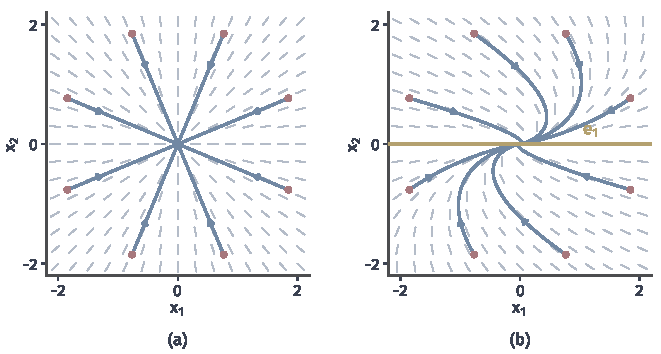
\includegraphics[width=112mm]{figures/06-differential-equations/01-ordinary-differential-equations/matplotlib/lde-jordan-vs-diagonal/figure.pdf}
  \caption{特征值相同而相图不同，红点是半径为$2$的圆上的初值。(a)$\bm{A}=-\bm{I}$，每个方向都是特征方向，轨线是直线。(b)$\bm{A}=\bm{J}$，只有黄色的$\bm{e}_1$轴是特征方向，其余轨线都沿它的方向进入原点。}
  \label{fig:lde-jordan-vs-diagonal}
\end{BookInlineFigure}

\begin{BookInlineFigure}
  \centering
  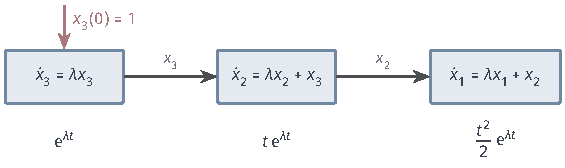
\includegraphics[width=96mm]{figures/06-differential-equations/01-ordinary-differential-equations/tikz/lde-jordan-chain/figure.pdf}
  \caption{三阶Jordan块看作一阶系统的串联。方框中是三个分量的方程，红色箭头表示只给$x_3$非零初值，方框下方是相应分量的响应。每一级的输入都含有该级自身的模式$\mathrm{e}^{\lambda t}$，于是响应多一次累积，得到$t$的更高次幂。}
  \label{fig:lde-jordan-chain}
\end{BookInlineFigure}

只看特征值还会错过有限时间内的放大。取
\[
 \bm{A}=\begin{bmatrix}-1&10\\0&-1\end{bmatrix},\qquad \bm{x}_0=\begin{bmatrix}0\\1\end{bmatrix}.
\]
把$\bm{N}$换成$10\bm{N}$，式~\eqref{eq:lde-jordan-exponential}给出
\[
 x_1(t)=10t\mathrm{e}^{-t},\qquad x_2(t)=\mathrm{e}^{-t}.
\]
两个特征值都是$-1$，看上去每个模式都在衰减，$x_1$却从$0$升到$t=1$处的$10/\mathrm{e}\approx3.68$，然后才下降，见图~\ref{fig:lde-jordan-transient}。放大来自对角线上方的耦合，特征值感受不到它。

\begin{BookInlineFigure}
  \centering
  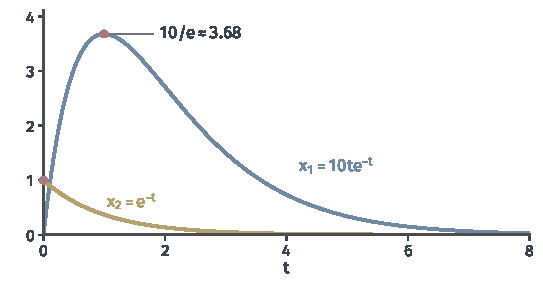
\includegraphics[width=92mm]{figures/06-differential-equations/01-ordinary-differential-equations/matplotlib/lde-jordan-transient/figure.pdf}
  \caption{重特征值带来的有限时间放大。$\bm{A}=\left[\begin{smallmatrix}-1&10\\0&-1\end{smallmatrix}\right]$，$\bm{x}_0=(0,1)^{\top}$。蓝线是$x_1$，在$t=1$达到峰值（右侧红点）；黄线是$x_2$，从左侧红点单调下降。}
  \label{fig:lde-jordan-transient}
\end{BookInlineFigure}

\paragraph{解的一般形状}
三角形式的回代可以写成一个对所有矩阵都成立的结论。

\begin{theorem}[矩阵指数的元素]
\label{thm:lde-exponential-shape}
设$\bm{A}\in\mathbb{R}^{n\times n}$的互异特征值为$\lambda_1,\ldots,\lambda_r$，代数重数为$m_1,\ldots,m_r$。则$\mathrm{e}^{t\bm{A}}$的每个元素都是下列函数的线性组合：
\begin{equation}
 t^j\mathrm{e}^{\lambda_it},\qquad 0\leq j<m_i,\quad i=1,\ldots,r.
 \label{eq:lde-exponential-shape}
\end{equation}
组合系数一般是复数。
\end{theorem}

\begin{proof}
由定理~\ref{thm:lde-matexp-properties}的(5)，只需证明上三角阵$\bm{T}$的情形。设$\bm{T}$的对角元为$\tau_1,\ldots,\tau_n$，解$\dot{\bm{x}}=\bm{T}\bm{x}$。从$i=n$往回归纳，证明$x_i$是若干$t^j\mathrm{e}^{\lambda t}$的组合，其中$\lambda\in\{\tau_i,\ldots,\tau_n\}$，$j$小于$\lambda$在$\tau_i,\ldots,\tau_n$中出现的次数。

$i=n$时$x_n=\mathrm{e}^{\tau_nt}x_n(0)$。设结论对$i+1,\ldots,n$成立。第$i$行是以$\sum_{k>i}T_{i,k}x_k$为输入的一阶线性方程，所以只要看一项输入$s^j\mathrm{e}^{\lambda s}$产生什么：
\[
 \int_0^t\mathrm{e}^{\tau_i(t-s)}s^j\mathrm{e}^{\lambda s}\,\mathrm{d}s=\mathrm{e}^{\tau_it}\int_0^ts^j\mathrm{e}^{(\lambda-\tau_i)s}\,\mathrm{d}s.
\]
若$\lambda\neq\tau_i$，分部积分$j$次得到次数至多为$j$的多项式乘$\mathrm{e}^{\lambda t}$，再加常数乘$\mathrm{e}^{\tau_it}$，幂次不升。若$\lambda=\tau_i$，积分等于$t^{j+1}/(j+1)$，幂次升一，而$\tau_i$在列表中恰好多出现一次。两种情形都保持归纳假设。
\end{proof}

定理说明指数、振荡和多项式因子是常系数线性系统仅有的三种成分：实部给出指数，虚部给出振荡，重根可能给出多项式。这里的“可能”不能省略，$-\bm{I}$就没有多项式因子。利用Jordan标准形可以把幂次上限收紧为“$j$小于$\lambda_i$的最大Jordan块阶数”，Jordan标准形的存在性证明较长，读者可查阅线性代数教材。

特征值的实部决定解在$t\to\infty$时的走向，但判断长期稳定还要考虑实部为零的特征值和Jordan块的大小，也要处理非线性系统，相关判据可参考\BookChapterRef{chap:dynamical-systems-long-term}{卷九第1章“动力系统与轨迹的长期行为”}。本章只关心解在有限时间上的形状。

\subsection{高阶标量方程}
\label{sec:lde-high-order}

质点在弹簧上的振动由二阶方程描述，电路和梁的问题还会出现更高阶的方程。记$\mathrm{D}=\mathrm{d}/\mathrm{d}t$，常系数$n$阶线性方程写作
\begin{equation}
 \mathrm{D}^nx+a_{n-1}\mathrm{D}^{n-1}x+\cdots+a_1\mathrm{D}x+a_0x=g(t),
 \label{eq:lde-high-order}
\end{equation}
其中系数$a_0,\ldots,a_{n-1}$是实常数。初值要给齐$x,\mathrm{D}x,\ldots,\mathrm{D}^{n-1}x$在$t_0$的值，共$n$个数。多项式$p(z)=z^n+a_{n-1}z^{n-1}+\cdots+a_0$称为方程的特征多项式，于是方程可以简写成$p(\mathrm{D})x=g$。

\paragraph{状态降阶}
第~\ref{chap:ordinary-differential-equations}章用位移和速度描述摆的状态，高阶方程也一样。令$x_k=\mathrm{D}^{k-1}x$（$k=1,\ldots,n$），前$n-1$个分量的方程就是定义$\dot{x}_k=x_{k+1}$，最后一个分量由方程~\eqref{eq:lde-high-order}解出。写成矩阵形式：
\begin{equation}
 \dot{\bm{x}}=\bm{C}\bm{x}+g(t)\bm{e}_n,\qquad
 \bm{C}=\begin{bmatrix}0&1&&\\&\ddots&\ddots&\\&&0&1\\-a_0&-a_1&\cdots&-a_{n-1}\end{bmatrix}.
 \label{eq:lde-companion}
\end{equation}
$\bm{C}$称为\term{友矩阵}（companion matrix）。例~\ref{ex:lde-running-system}的矩阵正是$p(z)=z^2+3z+2$的友矩阵。

图~\ref{fig:lde-companion-chain}把$n=3$的情形画成积分器串联。每个积分器保存一个状态分量，也就是系统需要“记住”的一个量，这也解释了为什么要给$n$个初值。

\begin{BookInlineFigure}
  \centering
  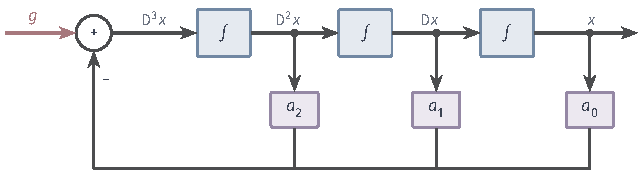
\includegraphics[width=108mm]{figures/06-differential-equations/01-ordinary-differential-equations/tikz/lde-companion-chain/figure.pdf}
  \caption{三阶方程$\mathrm{D}^3x+a_2\mathrm{D}^2x+a_1\mathrm{D}x+a_0x=g$的状态结构。蓝框是积分器，输出依次为状态分量$\mathrm{D}^2x,\mathrm{D}x,x$；紫框是系数，反馈后与红色输入$g$在求和点相减，得到最高阶导数。}
  \label{fig:lde-companion-chain}
\end{BookInlineFigure}

\begin{lemma}[友矩阵的谱]
\label{lem:lde-companion}
$\bm{C}$的特征多项式是$p$。对$\bm{C}$的每个特征值$\lambda$，特征子空间都是一维的，由下面的向量张成：
\begin{equation}
 \bm{v}(\lambda)=(1,\lambda,\lambda^2,\ldots,\lambda^{n-1})^{\top}.
 \label{eq:lde-companion-eigenvector}
\end{equation}
\end{lemma}

\begin{proof}
把$z\bm{I}-\bm{C}$的第$k$列乘$z^{k-1}$加到第$1$列（$k=2,\ldots,n$），行列式不变。逐行计算，新的第$1$列是$(0,\ldots,0,p(z))^{\top}$。

沿第$1$列展开，代数余子式对应的$n-1$阶子矩阵是下三角阵，对角元全为$-1$，行列式为$(-1)^{n-1}$。它再乘符号$(-1)^{n+1}$，结果是
\[
 \det(z\bm{I}-\bm{C})=(-1)^{n+1}(-1)^{n-1}p(z)=p(z).
\]

设$\bm{C}\bm{v}=\lambda\bm{v}$。前$n-1$行给出$v_{k+1}=\lambda v_k$，所以$\bm{v}$由$v_1$决定，并且$\bm{v}=v_1\bm{v}(\lambda)$。这就是特征子空间的一维性。
\end{proof}

引理的第二部分有直接的后果：若$\lambda$是$p$的$m$重根，$\bm{C}$在$\lambda$上只有一个Jordan块，阶数就是$m$。所以高阶标量方程不可能出现$-\bm{I}$那样“重特征值却没有多项式因子”的情况，重根一定带来$t,\ldots,t^{m-1}$。

\paragraph{基本解的列表}
上面的结论也可以直接从算子分解得到。常系数算子彼此可交换，$p(\mathrm{D})$可按根分解。关键的计算只有一步：
\[
 (\mathrm{D}-\lambda)\bigl(t^j\mathrm{e}^{\lambda t}\bigr)=jt^{j-1}\mathrm{e}^{\lambda t}.
\]
每作用一次$\mathrm{D}-\lambda$，$t$的幂次降一，所以$(\mathrm{D}-\lambda)^m$把$t^j\mathrm{e}^{\lambda t}$（$j<m$）变成零。

\begin{theorem}[高阶齐次方程的基本解]
\label{thm:lde-high-order-basis}
设$p(z)=\prod_{i=1}^{r}(z-\lambda_i)^{m_i}$，$\lambda_i$互异，$\sum_im_i=n$。则方程$p(\mathrm{D})x=0$的复值解构成$n$维线性空间，下列$n$个函数是它的一组基：
\begin{equation}
 t^j\mathrm{e}^{\lambda_it},\qquad 0\leq j<m_i,\quad i=1,\ldots,r.
 \label{eq:lde-high-order-basis}
\end{equation}
系数为实数时，一对共轭根$\alpha\pm\mathrm{i}\beta$对应的函数可以换成实函数$t^j\mathrm{e}^{\alpha t}\cos\beta t$和$t^j\mathrm{e}^{\alpha t}\sin\beta t$。
\end{theorem}

\begin{proof}
由上面的计算，这$n$个函数都是解。解空间的维数是$n$：由定理~\ref{thm:lde-constant-solution}，把解对应到初始状态$(x(0),\ldots,\mathrm{D}^{n-1}x(0))$是线性双射。

只需证明线性无关。假设存在非平凡关系$\sum_{i=1}^{r}q_i(t)\mathrm{e}^{\lambda_it}=0$，其中多项式$q_i$都不为零，$\lambda_i$互异，并取其中$r$最小的一个。$r=1$时$q_1\equiv0$，矛盾。

设$r\geq2$。乘$\mathrm{e}^{-\lambda_rt}$，再求导$\deg q_r+1$次，把$q_r$消去。其余每一项形如$q\mathrm{e}^{\mu t}$，$\mu=\lambda_i-\lambda_r\neq0$，而
\[
 \mathrm{D}(q\mathrm{e}^{\mu t})=(\dot{q}+\mu q)\mathrm{e}^{\mu t}.
\]
多项式的次数不变，首项系数乘$\mu$。所以得到一个只有$r-1$个指数的非平凡关系，与$r$的最小性矛盾。

系数为实数时，共轭根成对出现且重数相同。$t^j\mathrm{e}^{\alpha t}\cos\beta t$和$t^j\mathrm{e}^{\alpha t}\sin\beta t$分别是$t^j\mathrm{e}^{(\alpha\pm\mathrm{i}\beta)t}$的半和与半差（后者再除以$\mathrm{i}$），两组函数张成同一个空间。
\end{proof}

\paragraph{二阶振动方程}
质点受弹簧恢复力和阻尼时，满足$\ddot{x}+b\dot{x}+cx=0$，其中$b,c$是正常数。特征方程$z^2+bz+c=0$的判别式把运动分成三类。下面三个例子都取$x(0)=1$、$\dot{x}(0)=0$，只改变根的形状。

实根$p(z)=z^2+3z+2$，根为$-1,-2$。设$x=C_1\mathrm{e}^{-t}+C_2\mathrm{e}^{-2t}$，初值给出$C_1+C_2=1$和$-C_1-2C_2=0$，于是
\[
 x(t)=2\mathrm{e}^{-t}-\mathrm{e}^{-2t}.
\]

重根$p(z)=z^2+2z+1$，根为$-1$（二重）。设$x=(C_1+C_2t)\mathrm{e}^{-t}$，初值给出$C_1=1$和$-C_1+C_2=0$，于是
\[
 x(t)=(1+t)\mathrm{e}^{-t}.
\]

复根$p(z)=z^2+2z+5$，根为$-1\pm2\mathrm{i}$。设$x=\mathrm{e}^{-t}(C_1\cos2t+C_2\sin2t)$，初值给出$C_1=1$和$-C_1+2C_2=0$，于是
\[
 x(t)=\mathrm{e}^{-t}\Bigl(\cos2t+\frac12\sin2t\Bigr).
\]

图~\ref{fig:lde-damped-cases}比较这三条曲线。实根时质点单调回到平衡位置，复根时越过平衡位置来回摆动。重根恰好是两种情形的分界，它没有越过平衡位置，多项式因子$1+t$让它在开始阶段下降得比实根情形慢。三种情形及其物理名称见表~\ref{tab:lde-second-order}。

\begin{BookInlineFigure}
  \centering
  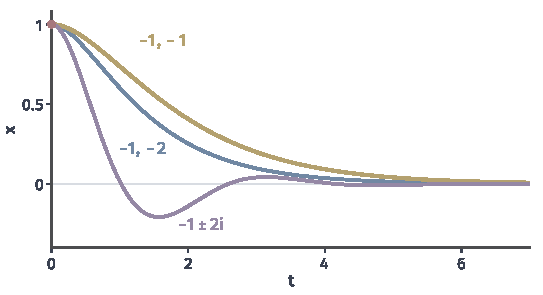
\includegraphics[width=92mm]{figures/06-differential-equations/01-ordinary-differential-equations/matplotlib/lde-damped-cases/figure.pdf}
  \caption{同一初值$x(0)=1$、$\dot{x}(0)=0$（红点）下的三类二阶方程，线旁标注特征根。蓝线：实根$-1,-2$。黄线：重根$-1,-1$。紫线：复根$-1\pm2\mathrm{i}$。}
  \label{fig:lde-damped-cases}
\end{BookInlineFigure}

\begin{BookInlineTable}
  \centering
  \caption{二阶常系数齐次方程的三类根。}
  \label{tab:lde-second-order}
  \begin{tabular}{lll}
    \toprule
    根的形状 & 基本解 & 运动形式\\
    \midrule
    相异实根$\lambda_1,\lambda_2$ & $\mathrm{e}^{\lambda_1t},\ \mathrm{e}^{\lambda_2t}$ & 过阻尼：不振荡\\
    二重根$\lambda$ & $\mathrm{e}^{\lambda t},\ t\mathrm{e}^{\lambda t}$ & 临界阻尼：不振荡的边界\\
    共轭复根$\alpha\pm\mathrm{i}\beta$ & $\mathrm{e}^{\alpha t}\cos\beta t,\ \mathrm{e}^{\alpha t}\sin\beta t$ & 欠阻尼：衰减振荡\\
    \bottomrule
  \end{tabular}
\end{BookInlineTable}

\paragraph{重根是两个根相撞}
重根的$t\mathrm{e}^{\lambda t}$看上去来得突然，用连续变化的系数看却很自然。考虑$\ddot{x}+2c\dot{x}+x=0$，根为$-c\pm\sqrt{c^2-1}$。图~\ref{fig:lde-root-locus}(a)显示，$c$从$0$增大到$1$时，一对共轭根沿单位圆向左靠拢，在$c=1$相撞于$-1$，然后沿实轴分开。

相撞时两个基本解变成同一个函数，线性无关性似乎丢失了。补救办法是取差商。令两根为$-1$和$-1-\varepsilon$，它们的基本解之差除以$\varepsilon$仍是解，而
\[
 \lim_{\varepsilon\to0}\frac{\mathrm{e}^{-t}-\mathrm{e}^{-(1+\varepsilon)t}}{\varepsilon}=t\mathrm{e}^{-t}.
\]
这个极限就是$\mathrm{e}^{\lambda t}$对$\lambda$的导数。图(b)中$\varepsilon$减小时差商曲线逐步靠近$t\mathrm{e}^{-t}$。两个靠得很近的根已经几乎产生了线性增长的因子，重根只是这个过程的极限。

\begin{BookInlineFigure}
  \centering
  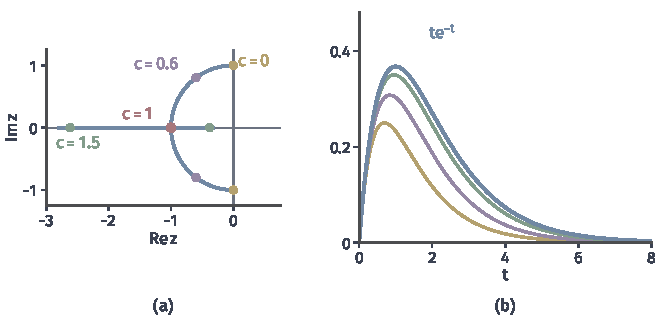
\includegraphics[width=112mm]{figures/06-differential-equations/01-ordinary-differential-equations/matplotlib/lde-root-locus/figure.pdf}
  \caption{根的相撞与多项式因子。(a)$z^2+2cz+1$的根随$c$的移动：$c=0$时在虚轴，$c=0.6$时在单位圆上，$c=1$时相撞于红点，$c=1.5$时分开在实轴上。(b)根为$-1,-1-\varepsilon$时的差商$(\mathrm{e}^{-t}-\mathrm{e}^{-(1+\varepsilon)t})/\varepsilon$，黄、紫、绿线依次取$\varepsilon=1,0.4,0.1$，蓝线是极限$t\mathrm{e}^{-t}$。}
  \label{fig:lde-root-locus}
\end{BookInlineFigure}


\section{时变系统}
\label{sec:lde-time-varying}

系数矩阵随时间变化时，方程变成
\begin{equation}
 \dot{\bm{x}}(t)=\bm{A}(t)\bm{x}(t),\qquad \bm{x}(s)=\bm{\xi},
 \label{eq:lde-time-varying}
\end{equation}
其中$\bm{A}:I\to\mathbb{R}^{n\times n}$在区间$I$上连续，$s\in I$。一个自然的想法是照搬标量公式，用$\exp\int_s^t\bm{A}$作传播。这个想法一般是错的，错在哪里要等传播矩阵本身建立好才能说清。所以先回答：不写闭式，能否定义出从时刻$s$到时刻$t$的线性传播？

\paragraph{用迭代造出传播矩阵}
把方程~\eqref{eq:lde-time-varying}对时间积分，得到
\[
 \bm{x}(t)=\bm{\xi}+\int_s^t\bm{A}(r)\bm{x}(r)\,\mathrm{d}r.
\]
解出现在右端，于是把右端的$\bm{x}$反复用整个等式代入。第一次代入后多出一项，第二次代入后再多一项，一直做下去，得到矩阵的级数
\begin{equation}
 \begin{aligned}
 \bm{\Phi}(t,s)={}&\bm{I}+\int_s^t\bm{A}(r_1)\,\mathrm{d}r_1\\
 &+\int_s^t\!\!\int_s^{r_1}\bm{A}(r_1)\bm{A}(r_2)\,\mathrm{d}r_2\,\mathrm{d}r_1+\cdots,
 \end{aligned}
 \label{eq:lde-peano-baker}
\end{equation}
称为\term{Peano--Baker级数}（Peano--Baker series）。第$k$项是$k$重积分，被积函数中时间较晚的因子写在左边。

这个级数是矩阵指数的时间排序版本。$\bm{A}$是常数时，第$k$项被积函数恒为$\bm{A}^k$，积分区域$s\leq r_k\leq\cdots\leq r_1\leq t$的体积是$(t-s)^k/k!$，第$k$项就是$(t-s)^k\bm{A}^k/k!$，级数回到式~\eqref{eq:lde-matrix-exponential}。阶乘的来历也清楚了：它是$k$个时刻按先后排列的区域在立方体中所占的比例。

\begin{definition}[状态转移矩阵]
\label{def:lde-transition}
设$\bm{A}$在$I$上连续，$s\in I$。把矩阵初值问题
\begin{equation}
 \partial_t\bm{\Phi}(t,s)=\bm{A}(t)\bm{\Phi}(t,s),\qquad \bm{\Phi}(s,s)=\bm{I}
 \label{eq:lde-transition}
\end{equation}
的解称为\term{状态转移矩阵}（state transition matrix）。第一个自变量$t$是终止时刻，第二个自变量$s$是初始时刻。
\end{definition}

\begin{theorem}[线性系统的整体存在唯一]
\label{thm:lde-transition-existence}
设$\bm{A}$在$I$上连续。对每个$s\in I$，问题~\eqref{eq:lde-transition}在整个$I$上有唯一解，由级数~\eqref{eq:lde-peano-baker}给出。对每个$\bm{\xi}\in\mathbb{R}^n$，方程~\eqref{eq:lde-time-varying}在$I$上的唯一解是
\begin{equation}
 \bm{x}(t)=\bm{\Phi}(t,s)\bm{\xi}.
 \label{eq:lde-transition-solution}
\end{equation}
\end{theorem}

\begin{proof}
取含$s$的紧子区间$J\subset I$，定义累积系数大小
\[
 \alpha(t)=\Bigl\lvert\int_s^t\lVert\bm{A}(r)\rVert_2\,\mathrm{d}r\Bigr\rvert.
\]
记级数第$k$项为$\bm{T}_k(t)$，它满足$\bm{T}_0=\bm{I}$和递推关系
\[
 \bm{T}_{k+1}(t)=\int_s^t\bm{A}(r)\bm{T}_k(r)\,\mathrm{d}r.
\]
归纳可得$\lVert\bm{T}_k(t)\rVert_2\leq\alpha(t)^k/k!$，归纳一步是
\[
 \lVert\bm{T}_{k+1}(t)\rVert_2\leq\Bigl\lvert\int_s^t\lVert\bm{A}(r)\rVert_2\frac{\alpha(r)^k}{k!}\,\mathrm{d}r\Bigr\rvert=\frac{\alpha(t)^{k+1}}{(k+1)!}.
\]

$\alpha$在$J$上有界，由优级数判别法，级数在$J$上一致收敛到连续的矩阵函数$\bm{\Phi}(\cdot,s)$。把递推式对$k$求和，并在一致收敛下交换求和与积分，得到
\[
 \bm{\Phi}(t,s)=\bm{I}+\int_s^t\bm{A}(r)\bm{\Phi}(r,s)\,\mathrm{d}r.
\]
被积函数连续，所以$\bm{\Phi}$对$t$连续可微，满足式~\eqref{eq:lde-transition}。$J$可以任取，所以解在整个$I$上存在。

再证唯一。设向量函数$\bm{y}$满足$\dot{\bm{y}}=\bm{A}\bm{y}$、$\bm{y}(s)=\bm{0}$，令$B=\max_J\lVert\bm{y}\rVert_2$。积分形式给出$\lVert\bm{y}(t)\rVert_2\leq B\alpha(t)$，代回积分形式再估计，反复进行，得到对每个$k$都有
\[
 \lVert\bm{y}(t)\rVert_2\leq\frac{B\alpha(t)^k}{k!}.
\]
令$k\to\infty$得$\bm{y}\equiv\bm{0}$。把它用于两个解之差，矩阵方程按列处理，就得到两个问题解的唯一性。式~\eqref{eq:lde-transition-solution}满足方程~\eqref{eq:lde-time-varying}可以直接代入验证。
\end{proof}

第~\ref{chap:ode-existence-continuation}章会把同样的迭代用于非线性方程，那里一般只能得到局部结论。线性方程的估计不受状态大小的影响，所以结论对整个$I$成立。若$\bm{A}$只是分段连续，就在每一段上求解，并在接缝处把状态接起来，$\bm{\Phi}$仍然连续，只是对$t$的导数在接缝处有跳变。

\paragraph{基本解矩阵}
实际求解时，往往是先设法找到$n$个线性无关的解，再组装成传播矩阵。

\begin{definition}[基本解矩阵]
\label{def:lde-fundamental-matrix}
若矩阵函数$\bm{X}:I\to\mathbb{R}^{n\times n}$连续可微，满足下式，并且在某一时刻可逆，就称它为\term{基本解矩阵}（fundamental matrix）：
\begin{equation}
 \dot{\bm{X}}(t)=\bm{A}(t)\bm{X}(t).
 \label{eq:lde-fundamental-matrix}
\end{equation}
\end{definition}

它的$n$列是$n$个解。若$\bm{X}$在某时刻$t_*$可逆，则它在每个时刻都可逆。否则存在时刻$t_1$和$\bm{c}\neq\bm{0}$使$\bm{X}(t_1)\bm{c}=\bm{0}$；而$\bm{X}(t)\bm{c}$是解，在$t_1$为零，由唯一性恒为零，这与$\bm{X}(t_*)$可逆矛盾。

由定义~\ref{def:lde-transition}的唯一性，$\bm{X}(t)\bm{X}(s)^{-1}$就是$\bm{\Phi}(t,s)$，因为它对$t$满足同一方程，在$t=s$时等于$\bm{I}$：
\begin{equation}
 \bm{\Phi}(t,s)=\bm{X}(t)\bm{X}(s)^{-1}.
 \label{eq:lde-fundamental-to-transition}
\end{equation}

这个公式可以理解为换坐标。$\bm{X}(s)^{-1}$把时刻$s$的状态写成$n$个基本解在该时刻取值的组合，得到组合系数。方程是线性的，组合系数不随时间改变。再用时刻$t$的基本解按同样的系数组合，就读出了时刻$t$的状态。

\begin{theorem}[状态转移矩阵的性质]
\label{thm:lde-transition-properties}
对$r,s,t\in I$，下列性质成立，时刻的大小次序不限。
\begin{enumerate}
 \item 复合：
 \begin{equation}
  \bm{\Phi}(t,r)\bm{\Phi}(r,s)=\bm{\Phi}(t,s).
  \label{eq:lde-transition-composition}
 \end{equation}
 \item 可逆：$\bm{\Phi}(t,s)$可逆，并且
 \begin{equation}
  \bm{\Phi}(t,s)^{-1}=\bm{\Phi}(s,t).
  \label{eq:lde-transition-inverse}
 \end{equation}
 \item 对初始时刻求导：
 \begin{equation}
  \partial_s\bm{\Phi}(t,s)=-\bm{\Phi}(t,s)\bm{A}(s).
  \label{eq:lde-transition-initial-derivative}
 \end{equation}
 \item 常系数情形：若$\bm{A}(t)\equiv\bm{A}$，则$\bm{\Phi}$只依赖$t-s$：
 \begin{equation}
  \bm{\Phi}(t,s)=\mathrm{e}^{(t-s)\bm{A}}.
  \label{eq:lde-transition-constant}
 \end{equation}
\end{enumerate}
\end{theorem}

\begin{proof}
取$\bm{X}(t)=\bm{\Phi}(t,t_*)$作为基本解矩阵，其中$t_*\in I$任意。代入式~\eqref{eq:lde-fundamental-to-transition}，(1)就是
\[
 \bm{X}(t)\bm{X}(r)^{-1}\bm{X}(r)\bm{X}(s)^{-1}=\bm{X}(t)\bm{X}(s)^{-1}.
\]
(2)由$\bm{X}(s)\bm{X}(t)^{-1}$是$\bm{X}(t)\bm{X}(s)^{-1}$的逆得到。

(3)对$\bm{X}(s)^{-1}\bm{X}(s)=\bm{I}$求导，得到恒等式
\[
 \partial_s\bigl(\bm{X}(s)^{-1}\bigr)=-\bm{X}(s)^{-1}\dot{\bm{X}}(s)\bm{X}(s)^{-1}.
\]
代入$\dot{\bm{X}}=\bm{A}\bm{X}$，并左乘$\bm{X}(t)$，得
\[
 \partial_s\bm{\Phi}(t,s)=-\bm{X}(t)\bm{X}(s)^{-1}\bm{A}(s)=-\bm{\Phi}(t,s)\bm{A}(s).
\]

(4)由定理~\ref{thm:lde-constant-solution}，$\mathrm{e}^{(t-s)\bm{A}}$满足式~\eqref{eq:lde-transition}，由唯一性得结论。
\end{proof}

两个时刻的角色并不对称。对终止时刻求导，系数矩阵$\bm{A}(t)$乘在左边，表示最后这一小段的传播作用在最外层。对初始时刻求导，$-\bm{A}(s)$乘在右边，表示最开始的那一小段被去掉。图~\ref{fig:lde-transition-composition}是复合关系的示意：先从$s$传到$r$，再从$r$传到$t$，与直接从$s$传到$t$结果相同。

\begin{BookInlineFigure}
  \centering
  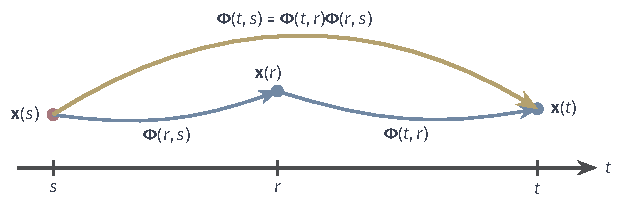
\includegraphics[width=105mm]{figures/06-differential-equations/01-ordinary-differential-equations/tikz/lde-transition-composition/figure.pdf}
  \caption{状态转移矩阵的复合。横轴是时间，红点是时刻$s$的状态，蓝点是其后的状态。两段蓝色箭头依次传播，黄色箭头直接传播，二者结果相同。矩阵乘积中晚的时刻写在左边。}
  \label{fig:lde-transition-composition}
\end{BookInlineFigure}

\begin{example}[一个可解的时变系统]
\label{ex:lde-time-varying}
取
\[
 \bm{A}(t)=\begin{bmatrix}0&t\\0&1\end{bmatrix},
\]
方程是$\dot{x}_1=tx_2$、$\dot{x}_2=x_2$。第二个方程先解出$x_2=\mathrm{e}^{t}x_2(0)$。代入第一个方程，再用分部积分，可知$t\mathrm{e}^{t}$的一个原函数是$(t-1)\mathrm{e}^{t}$。

于是$(1,0)^{\top}$和$((t-1)\mathrm{e}^{t},\mathrm{e}^{t})^{\top}$是两个解，把它们并排放置，得到基本解矩阵和它的逆：
\[
 \bm{X}(t)=\begin{bmatrix}1&(t-1)\mathrm{e}^{t}\\0&\mathrm{e}^{t}\end{bmatrix},\qquad
 \bm{X}(s)^{-1}=\begin{bmatrix}1&1-s\\0&\mathrm{e}^{-s}\end{bmatrix}.
\]
由式~\eqref{eq:lde-fundamental-to-transition}，
\[
 \bm{\Phi}(t,s)=\begin{bmatrix}1&(1-s)+(t-1)\mathrm{e}^{t-s}\\0&\mathrm{e}^{t-s}\end{bmatrix}.
\]
取$t=s$，右上角为$(1-s)+(s-1)=0$，符合$\bm{\Phi}(s,s)=\bm{I}$。再取时长都是$1$的两段：
\[
 \bm{\Phi}(1,0)=\begin{bmatrix}1&1\\0&\mathrm{e}\end{bmatrix},\qquad
 \bm{\Phi}(2,1)=\begin{bmatrix}1&\mathrm{e}\\0&\mathrm{e}\end{bmatrix}.
\]
它们不相等，说明传播同时依赖两个时刻，而不只依赖时长。它们的乘积是
\[
 \bm{\Phi}(2,1)\bm{\Phi}(1,0)=\begin{bmatrix}1&1+\mathrm{e}^2\\0&\mathrm{e}^2\end{bmatrix},
\]
这正是公式给出的$\bm{\Phi}(2,0)$，复合关系得到验证。
\end{example}

\paragraph{为什么不能积分后取指数}
现在可以检验开始时的想法了。对例~\ref{ex:lde-time-varying}的系数，从$0$积分得到
\[
 \bm{M}(t)=\int_0^t\bm{A}(r)\,\mathrm{d}r=\begin{bmatrix}0&t^2/2\\0&t\end{bmatrix}.
\]
固定$t$，写$\bm{M}=t\bm{B}$，其中$\bm{B}$满足$\bm{B}^2=\bm{B}$：
\[
 \bm{B}=\begin{bmatrix}0&t/2\\0&1\end{bmatrix}.
\]
于是级数中$\bm{B}^k$全部等于$\bm{B}$，求和得到
\[
 \mathrm{e}^{\bm{M}(t)}=\bm{I}+(\mathrm{e}^{t}-1)\bm{B}=\begin{bmatrix}1&(\mathrm{e}^{t}-1)t/2\\0&\mathrm{e}^{t}\end{bmatrix}.
\]

把它与$\bm{\Phi}(t,0)$的右上角比较：真解是$(t-1)\mathrm{e}^{t}+1$，直接取指数的结果是$(\mathrm{e}^{t}-1)t/2$。取$t=2$，前者是$\mathrm{e}^2+1\approx8.389$，后者是$\mathrm{e}^2-1\approx6.389$。图~\ref{fig:lde-noncommuting}中两条曲线随时间逐渐分开，绿点是对原方程作数值积分的结果，它落在蓝线上。

\begin{BookInlineFigure}
  \centering
  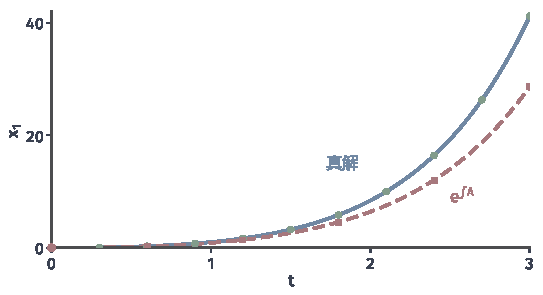
\includegraphics[width=92mm]{figures/06-differential-equations/01-ordinary-differential-equations/matplotlib/lde-noncommuting/figure.pdf}
  \caption{时变系统不能对系数积分后直接取指数。$\bm{A}(t)=\left[\begin{smallmatrix}0&t\\0&1\end{smallmatrix}\right]$，$\bm{x}(0)=(0,1)^{\top}$，图中是分量$x_1$。蓝线是真解$(t-1)\mathrm{e}^{t}+1$，绿点是步长$0.05$的四阶Runge--Kutta数值解；红色虚线是$\exp\int_0^t\bm{A}$给出的$(\mathrm{e}^{t}-1)t/2$，红色方点是对$\bm{M}(t)$直接计算矩阵指数的结果。}
  \label{fig:lde-noncommuting}
\end{BookInlineFigure}

失败的原因在求导。若想让$\mathrm{e}^{\bm{M}(t)}$满足方程，$\mathrm{e}^{\bm{M}}$的导数就要等于$\dot{\bm{M}}\mathrm{e}^{\bm{M}}$。看级数中的二次项：
\[
 \frac{\mathrm{d}}{\mathrm{d}t}\bm{M}^2=\dot{\bm{M}}\bm{M}+\bm{M}\dot{\bm{M}}.
\]
只有$\dot{\bm{M}}$与$\bm{M}$可交换时，它才等于$2\dot{\bm{M}}\bm{M}$。例中$\bm{A}(s)\bm{A}(t)=\bm{A}(s)$而$\bm{A}(t)\bm{A}(s)=\bm{A}(t)$，两个时刻的系数不可交换。

从传播的角度看更直观。$\exp\int\bm{A}$把各时刻的系数不分先后地加在一起，Peano--Baker级数却严格保留“晚的在左”的次序。图~\ref{fig:lde-switching-order}用两段常系数的切换说明次序的影响。设两段系数各作用单位时间：
\[
 \bm{A}_1=\begin{bmatrix}0&1\\0&0\end{bmatrix},\qquad \bm{A}_2=\begin{bmatrix}0&0\\1&0\end{bmatrix}.
\]
由$\bm{A}_1^2=\bm{A}_2^2=\bm{0}$，得$\mathrm{e}^{\bm{A}_i}=\bm{I}+\bm{A}_i$。

先用$\bm{A}_1$、后用$\bm{A}_2$的传播是
\[
 \mathrm{e}^{\bm{A}_2}\mathrm{e}^{\bm{A}_1}=\begin{bmatrix}1&1\\1&2\end{bmatrix}.
\]
次序反过来的传播是
\[
 \mathrm{e}^{\bm{A}_1}\mathrm{e}^{\bm{A}_2}=\begin{bmatrix}2&1\\1&1\end{bmatrix}.
\]
两种切换的系数积分都是$\bm{A}_1+\bm{A}_2$，而直接取指数得到
\[
 \mathrm{e}^{\bm{A}_1+\bm{A}_2}=\begin{bmatrix}\cosh1&\sinh1\\\sinh1&\cosh1\end{bmatrix},
\]
与两者都不同。这就像先向右剪切再向上剪切，与先向上剪切再向右剪切，结果是两个不同的平行四边形。

\begin{BookInlineFigure}
  \centering
  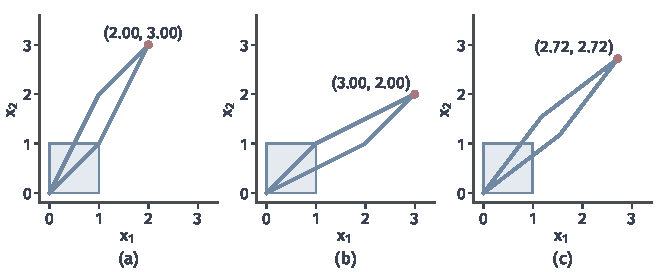
\includegraphics[width=112mm]{figures/06-differential-equations/01-ordinary-differential-equations/matplotlib/lde-switching-order/figure.pdf}
  \caption{切换次序影响结果，浅蓝方块是单位正方形，蓝线是它的像，红点是$(1,1)^{\top}$的像。(a)$\mathrm{e}^{\bm{A}_2}\mathrm{e}^{\bm{A}_1}$。(b)$\mathrm{e}^{\bm{A}_1}\mathrm{e}^{\bm{A}_2}$。(c)$\mathrm{e}^{\bm{A}_1+\bm{A}_2}$，它对应系数积分后直接取指数，不等于任何一种切换次序的实际传播。}
  \label{fig:lde-switching-order}
\end{BookInlineFigure}

\paragraph{可交换时的简化}
上面的分析也指出了简化公式成立的条件：让所有时刻的系数彼此可交换。

\begin{theorem}[可交换系数的状态转移矩阵]
\label{thm:lde-commuting}
设$\bm{A}$在$I$上连续，并且对任意$r,r'\in I$都有$\bm{A}(r)\bm{A}(r')=\bm{A}(r')\bm{A}(r)$。则
\begin{equation}
 \bm{\Phi}(t,s)=\exp\Bigl(\int_s^t\bm{A}(r)\,\mathrm{d}r\Bigr).
 \label{eq:lde-commuting}
\end{equation}
\end{theorem}

\begin{proof}
固定$s$，令$\bm{M}(t)=\int_s^t\bm{A}(r)\,\mathrm{d}r$。积分是Riemann和的极限，而每个Riemann和都与$\bm{A}(t)$可交换，所以$\bm{M}(t)\bm{A}(t)=\bm{A}(t)\bm{M}(t)$。

用乘积求导并归纳，$\frac{\mathrm{d}}{\mathrm{d}t}\bm{M}^k$是$k$项之和，每一项都把一个因子$\bm{M}$换成$\bm{A}(t)$。交换关系把$\bm{A}(t)$移到最左边，得到
\[
 \frac{\mathrm{d}}{\mathrm{d}t}\bm{M}^k=k\bm{A}(t)\bm{M}^{k-1}.
\]
逐项求导的级数在紧子区间上被$\lVert\bm{A}(t)\rVert_2\mathrm{e}^{\lVert\bm{M}(t)\rVert_2}$的同型优级数控制，所以求导合法，并且
\[
 \frac{\mathrm{d}}{\mathrm{d}t}\mathrm{e}^{\bm{M}(t)}=\bm{A}(t)\mathrm{e}^{\bm{M}(t)}.
\]
又有$\bm{M}(s)=\bm{0}$，由定理~\ref{thm:lde-transition-existence}的唯一性得到结论。
\end{proof}

定理的条件是充分条件。标量方程、对角系数和$\bm{A}(t)=a(t)\bm{B}$（$\bm{B}$为常矩阵）都满足它。最后一种情形有直观的含义：$a(t)$只决定沿$\bm{B}$的轨线走得多快，不改变轨线本身。例如$\bm{A}(t)=2t\bm{J}_0$时，式~\eqref{eq:lde-commuting}给出
\[
 \bm{\Phi}(t,0)=\mathrm{e}^{t^2\bm{J}_0}=\begin{bmatrix}\cos t^2&\sin t^2\\-\sin t^2&\cos t^2\end{bmatrix}.
\]
状态仍在圆周上转动，只是把时间换成了$t^2$。一般的时变系统没有这种闭式，$\bm{\Phi}$要靠数值方法求解，这由第~\ref{chap:ode-numerical-methods}章讨论。


\section{非齐次方程}
\label{sec:lde-inhomogeneous}

齐次传播建立之后，再加入外部输入。设$\bm{A}$、$\bm{g}$在区间$I$上连续，考虑
\begin{equation}
 \dot{\bm{x}}(t)=\bm{A}(t)\bm{x}(t)+\bm{g}(t),\qquad \bm{x}(t_0)=\bm{x}_0.
 \label{eq:lde-inhomogeneous}
\end{equation}
输入在每一时刻都推动状态，推动的效果又随齐次系统继续传播。怎样把这两件事合写成一个公式？

\paragraph{常数变易}
没有输入时，解是$\bm{\Phi}(t,t_0)\bm{c}$，其中$\bm{c}$是常向量，等于初始状态。输入不断改变状态，可以理解为“初始状态”这个系数在缓慢漂移。于是让$\bm{c}$依赖时间，设$\bm{x}(t)=\bm{\Phi}(t,t_0)\bm{c}(t)$，代入方程。

乘积求导时，$\partial_t\bm{\Phi}$产生的项恰好是$\bm{A}\bm{x}$，与方程右端抵消，只剩下
\[
 \bm{\Phi}(t,t_0)\dot{\bm{c}}(t)=\bm{g}(t).
\]
用$\bm{\Phi}(t,t_0)^{-1}=\bm{\Phi}(t_0,t)$乘两边，再由$\bm{c}(t_0)=\bm{x}_0$积分，得到
\[
 \bm{c}(t)=\bm{x}_0+\int_{t_0}^{t}\bm{\Phi}(t_0,s)\bm{g}(s)\,\mathrm{d}s.
\]

这一步也有含义：$\bm{\Phi}(t_0,s)\bm{g}(s)$把时刻$s$的输入折算回初始时刻。把$\bm{c}(t)$代回去，再用复合关系$\bm{\Phi}(t,t_0)\bm{\Phi}(t_0,s)=\bm{\Phi}(t,s)$，就得到下面的定理。

\begin{theorem}[常数变易公式]
\label{thm:lde-variation-of-constants}
设$\bm{A},\bm{g}$在$I$上连续，$t_0\in I$。初值问题~\eqref{eq:lde-inhomogeneous}在$I$上有唯一解，它是
\begin{equation}
 \bm{x}(t)=\bm{\Phi}(t,t_0)\bm{x}_0+\int_{t_0}^{t}\bm{\Phi}(t,s)\bm{g}(s)\,\mathrm{d}s.
 \label{eq:lde-variation-of-constants}
\end{equation}
常系数时$\bm{\Phi}(t,s)=\mathrm{e}^{(t-s)\bm{A}}$，公式成为
\begin{equation}
 \bm{x}(t)=\mathrm{e}^{(t-t_0)\bm{A}}\bm{x}_0+\int_{t_0}^{t}\mathrm{e}^{(t-s)\bm{A}}\bm{g}(s)\,\mathrm{d}s.
 \label{eq:lde-duhamel-constant}
\end{equation}
\end{theorem}

\begin{proof}
先检验式~\eqref{eq:lde-variation-of-constants}满足方程和初值。由复合关系，这个公式可以写成乘积$\bm{\Phi}(t,t_0)\bm{c}(t)$，其中$\bm{c}$如上。对乘积求导，得
\[
\begin{aligned}
 \dot{\bm{x}}(t)&=\bm{A}(t)\bm{\Phi}(t,t_0)\bm{c}(t)+\bm{\Phi}(t,t_0)\bm{\Phi}(t_0,t)\bm{g}(t)\\
 &=\bm{A}(t)\bm{x}(t)+\bm{g}(t).
\end{aligned}
\]
$t=t_0$时积分为零，$\bm{\Phi}(t_0,t_0)=\bm{I}$，所以$\bm{x}(t_0)=\bm{x}_0$。

再证唯一。两个解之差满足齐次方程，初值为零，由定理~\ref{thm:lde-transition-existence}恒为零。
\end{proof}

式~\eqref{eq:lde-variation-of-constants}称为\term{常数变易公式}（variation of constants formula），也称\term{Duhamel公式}（Duhamel formula）。若$\bm{g}$只在每个紧子区间上可积，公式不变，解是局部绝对连续的，方程几乎处处成立，这与定理~\ref{thm:lde-scalar-integrable}的论证相同。

\paragraph{初始状态响应与零初值响应}
公式的两项分别只含一种数据。第一项$\bm{\Phi}(t,t_0)\bm{x}_0$不依赖输入，称为\term{零输入响应}（zero-input response）。第二项不依赖初始状态，称为\term{零状态响应}（zero-state response）。

每一项都线性依赖自己的数据，总响应是两项之和。所以“响应”对数据对$(\bm{x}_0,\bm{g})$是线性的。常见的误解是说总响应关于输入线性：若$\bm{x}_0\neq\bm{0}$，把输入加倍并不会把总响应加倍，因为零输入响应没有变。

\begin{example}[阶跃输入的响应分解]
\label{ex:lde-step-response}
考虑$\ddot{x}+3\dot{x}+2x=1$，$x(0)=1$，$\dot{x}(0)=0$。状态形式用例~\ref{ex:lde-running-system}的矩阵，$\bm{g}=(0,1)^{\top}$，$\bm{x}_0=(1,0)^{\top}$。零输入响应的第一分量已经算过，是$2\mathrm{e}^{-t}-\mathrm{e}^{-2t}$。

零状态响应用到$\mathrm{e}^{r\bm{A}}$的第二列，它的第一分量是$\mathrm{e}^{-r}-\mathrm{e}^{-2r}$。在式~\eqref{eq:lde-duhamel-constant}中令$r=t-s$，积分变成
\[
 \int_0^t(\mathrm{e}^{-r}-\mathrm{e}^{-2r})\,\mathrm{d}r=\frac12-\mathrm{e}^{-t}+\frac12\mathrm{e}^{-2t}.
\]
两部分相加，得到总响应
\[
 x(t)=\frac12+\mathrm{e}^{-t}-\frac12\mathrm{e}^{-2t}.
\]
代回检验：$x(0)=1$，$\dot{x}=-\mathrm{e}^{-t}+\mathrm{e}^{-2t}$，所以$\dot{x}(0)=0$；再求$\ddot{x}=\mathrm{e}^{-t}-2\mathrm{e}^{-2t}$，并计算
\[
 \ddot{x}+3\dot{x}+2x=(1-3+2)\mathrm{e}^{-t}+(-2+3-1)\mathrm{e}^{-2t}+1=1.
\]
\end{example}

图~\ref{fig:lde-response-decomposition}中，黄线由初始状态决定，从$1$下降到$0$；紫线由输入决定，从$0$升到$1/2$。蓝线是二者之和。这个系统的状态最终停在$1/2$，只和输入有关，初值的痕迹全部由零输入响应带走。

\begin{BookInlineFigure}
  \centering
  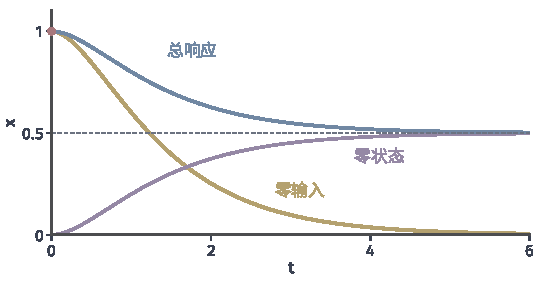
\includegraphics[width=92mm]{figures/06-differential-equations/01-ordinary-differential-equations/matplotlib/lde-response-decomposition/figure.pdf}
  \caption{响应的分解，方程$\ddot{x}+3\dot{x}+2x=1$，$x(0)=1$（红点），$\dot{x}(0)=0$。黄线是零输入响应，紫线是零状态响应，蓝线是总响应，灰色虚线是水平$1/2$。}
  \label{fig:lde-response-decomposition}
\end{BookInlineFigure}

\paragraph{受迫振动与共振}
荡秋千时，每次都在同一相位推一下，幅度就越来越大；推的节奏不对，推力再大也荡不高。把这个现象写成方程，就是无阻尼振子受周期外力：
\begin{equation}
 \ddot{x}+\omega_0^2x=\cos\omega t,\qquad x(0)=\dot{x}(0)=0,
 \label{eq:lde-forced-oscillator}
\end{equation}
其中$\omega_0>0$是固有频率，$\omega>0$是外力频率。

状态形式的系数矩阵如下，它满足$\bm{A}^2=-\omega_0^2\bm{I}$：
\[
 \bm{A}=\begin{bmatrix}0&1\\-\omega_0^2&0\end{bmatrix}.
\]
级数的偶次项和奇次项分别凑成余弦和正弦，得到
\[
 \mathrm{e}^{t\bm{A}}=\begin{bmatrix}\cos\omega_0t&\sin(\omega_0t)/\omega_0\\-\omega_0\sin\omega_0t&\cos\omega_0t\end{bmatrix}.
\]
输入是$(0,\cos\omega t)^{\top}$，所以式~\eqref{eq:lde-duhamel-constant}的第一分量是
\begin{equation}
 x(t)=\frac{1}{\omega_0}\int_0^t\sin\bigl(\omega_0(t-s)\bigr)\cos(\omega s)\,\mathrm{d}s.
 \label{eq:lde-forced-integral}
\end{equation}

用积化和差把被积函数拆开：
\[
 \begin{aligned}
 \sin(\omega_0(t-s))\cos\omega s={}&\tfrac12\sin\bigl(\omega_0t-(\omega_0-\omega)s\bigr)\\
 &+\tfrac12\sin\bigl(\omega_0t-(\omega_0+\omega)s\bigr).
 \end{aligned}
\]
当$\omega\neq\omega_0$时，两项都对$s$积分，第一项给出$(\cos\omega t-\cos\omega_0t)/(\omega_0-\omega)$，第二项给出$(\cos\omega t-\cos\omega_0t)/(\omega_0+\omega)$。代入式~\eqref{eq:lde-forced-integral}并通分，
\begin{equation}
 x(t)=\frac{\cos\omega t-\cos\omega_0t}{\omega_0^2-\omega^2},\qquad \omega\neq\omega_0.
 \label{eq:lde-off-resonance}
\end{equation}
这个解有界，幅度不超过$2/\lvert\omega_0^2-\omega^2\rvert$。$\omega$接近$\omega_0$时，两个余弦的频率相近，交替增强与抵消，形成缓慢起伏的\term{拍}（beat）。

当$\omega=\omega_0$时，第一项是常数$\tfrac12\sin\omega_0t$，它对$s$积分得到$\tfrac12t\sin\omega_0t$。第二项在$[0,t]$上的积分为
\[
 \frac12\Bigl[\frac{\cos(\omega_0t-2\omega_0s)}{2\omega_0}\Bigr]_{s=0}^{s=t}=0.
\]
于是
\begin{equation}
 x(t)=\frac{t\sin\omega_0t}{2\omega_0},\qquad \omega=\omega_0.
 \label{eq:lde-resonance}
\end{equation}
代回检验，取$\omega_0=1$，$x=\tfrac12t\sin t$。两次求导得到
\[
 \dot{x}=\frac{\sin t+t\cos t}{2},\qquad \ddot{x}=\cos t-\frac{t\sin t}{2}.
\]
所以$\ddot{x}+x=\cos t$，并且$x(0)=\dot{x}(0)=0$。

这种振幅按$t$线性增长的现象称为\term{共振}（resonance）。图~\ref{fig:lde-resonance}取$\omega_0=1$比较三种外力频率。外力大小完全相同，差别只在频率：$\omega=2$时响应很小，$\omega=1.2$时出现拍，$\omega=1$时振幅沿紫色虚线$\pm t/2$增长。

\begin{BookInlineFigure}
  \centering
  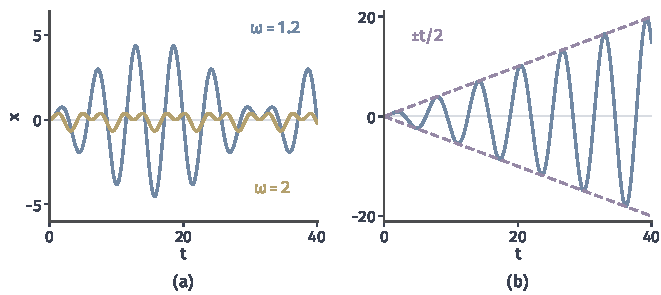
\includegraphics[width=112mm]{figures/06-differential-equations/01-ordinary-differential-equations/matplotlib/lde-resonance/figure.pdf}
  \caption{方程~\eqref{eq:lde-forced-oscillator}取$\omega_0=1$的零初值响应。(a)$\omega=2$（黄）的响应有界，$\omega=1.2$（蓝）出现拍。(b)$\omega=1$时发生共振，响应$t\sin t/2$的振幅沿紫色虚线$\pm t/2$线性增长。}
  \label{fig:lde-resonance}
\end{BookInlineFigure}

共振的原因要看积分~\eqref{eq:lde-forced-integral}的被积函数。$\sin(\omega_0(t-s))$是时刻$s$的单位冲击到时刻$t$还留下的响应，$\cos\omega s$是那一刻的外力。图~\ref{fig:lde-resonance-integrand}固定$t=4.5\pi$，画出被积函数对$s$的形状。

$\omega=1$时被积函数不变号，每一时刻的贡献都同向累加，面积是$t/2\approx7.07$。$\omega=2$时正负面积大部分抵消，只剩$1/3$。所以共振并不是输入太大，而是输入与齐次模式同频，各时刻留下的响应到达同一时刻时相位一致。

这与第~\ref{sec:lde-constant}节的多项式因子是同一个机制：Jordan链上一级的输出含有下一级自身的模式，这里外力含有振子自身的模式，于是都多出一个因子$t$。无阻尼模型的振幅没有上界。若有阻尼，齐次模式按指数衰减，早期输入留下的响应会逐渐消失，累积不再无限制地增长。

\begin{BookInlineFigure}
  \centering
  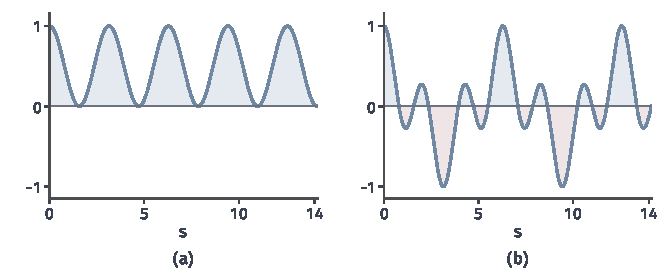
\includegraphics[width=112mm]{figures/06-differential-equations/01-ordinary-differential-equations/matplotlib/lde-resonance-integrand/figure.pdf}
  \caption{共振的累积机制。式~\eqref{eq:lde-forced-integral}取$\omega_0=1$、$t=4.5\pi$时的被积函数$\sin(t-s)\cos\omega s$，浅蓝为正面积，浅红为负面积。(a)$\omega=1$，被积函数不变号，积分约为$7.07$。(b)$\omega=2$，正负抵消，积分为$1/3$。}
  \label{fig:lde-resonance-integrand}
\end{BookInlineFigure}


\section{因果Green函数}
\label{sec:lde-green}

常数变易公式中，积分号里的$\bm{\Phi}(t,s)$单独拿出来是什么意思？做一个思想实验：系统原本静止，在时刻$s$突然敲它一下，随后观察它的响应。

\paragraph{窄脉冲的极限}
“敲一下”可以用一个窄而高的矩形输入来描述。取单位面积的脉冲：在$[s,s+\varepsilon)$上输入为$\varepsilon^{-1}\bm{e}_j$，其余时刻为零，$\bm{e}_j$是第$j$个坐标方向。以零初值代入式~\eqref{eq:lde-variation-of-constants}。输入开始前响应为零，输入结束后，当$t\geq s+\varepsilon$时，
\[
 \bm{x}_{\varepsilon}(t)=\frac{1}{\varepsilon}\int_s^{s+\varepsilon}\bm{\Phi}(t,r)\bm{e}_j\,\mathrm{d}r.
\]

由定理~\ref{thm:lde-transition-properties}的(3)，$\bm{\Phi}(t,r)$对$r$连续，所以$\varepsilon\to0$时积分平均趋于$r=s$处的值。对每个$t>s$，
\begin{equation}
 \lim_{\varepsilon\to0^+}\bm{x}_{\varepsilon}(t)=\bm{\Phi}(t,s)\bm{e}_j,
 \label{eq:lde-pulse-limit}
\end{equation}
而$t<s$时响应恒为零。$\bm{\Phi}(t,s)$的第$j$列就是这样一种响应：在时刻$s$沿第$j$个方向敲一下，系统在时刻$t$的状态。

\begin{definition}[因果Green函数]
\label{def:lde-causal-green}
对$t,s\in I$，线性系统$\dot{\bm{x}}=\bm{A}(t)\bm{x}+\bm{g}$的\term{因果Green函数}（causal Green's function）定义为
\begin{equation}
 \bm{G}(t,s)=\bm{\Phi}(t,s)\mathbb{I}_{[s,\infty)}(t),
 \label{eq:lde-causal-green}
\end{equation}
其中$\mathbb{I}_{[s,\infty)}$是区间$[s,\infty)$的示性函数。$\bm{G}(t,s)$在$t<s$时为零。
\end{definition}

有了$\bm{G}$，零状态响应（记为$\bm{x}_{\mathrm{zs}}$）可以写成对整段时间的积分。设$\bm{g}$在$[t_0,T]$上连续，$t\in[t_0,T]$，由$\bm{G}$在$s>t$时为零，得
\begin{equation}
 \bm{x}_{\mathrm{zs}}(t)=\int_{t_0}^{T}\bm{G}(t,s)\bm{g}(s)\,\mathrm{d}s.
 \label{eq:lde-green-solution}
\end{equation}
积分虽然延伸到$T$，实际只用到$s\leq t$的输入。这就是“因果”的含义：未来的输入不影响现在的状态。

$\bm{G}$在对角线$t=s$处有跳变。从$t<s$一侧的$\bm{0}$跳到$t>s$一侧的$\bm{I}$，所以
\begin{equation}
 \bm{G}(s^+,s)-\bm{G}(s^-,s)=\bm{I}.
 \label{eq:lde-green-jump}
\end{equation}
$t\neq s$时，$\bm{G}$对$t$满足齐次方程。工程和物理中常把这两条性质合写成
\[
 (\partial_t-\bm{A}(t))\bm{G}(t,s)=\delta(t-s)\bm{I}.
\]
这里的$\delta$不是普通函数，这个写法只是式~\eqref{eq:lde-pulse-limit}和跳变条件~\eqref{eq:lde-green-jump}的简写。

\paragraph{标量例子与脉冲响应}
常系数时$\bm{G}$只依赖时间差，$\bm{G}(t,s)=\bm{H}(t-s)$，其中
\begin{equation}
 \bm{H}(t)=\mathrm{e}^{t\bm{A}}\mathbb{I}_{[0,\infty)}(t).
 \label{eq:lde-constant-green}
\end{equation}
取$t_0=0$，零状态响应就是一个卷积：
\begin{equation}
 \bm{x}_{\mathrm{zs}}(t)=\int_0^t\bm{H}(t-s)\bm{g}(s)\,\mathrm{d}s.
 \label{eq:lde-convolution-response}
\end{equation}
时变系统没有这个简化。例如$\dot{x}=-2tx+g$的Green函数是
\[
 G(t,s)=\mathrm{e}^{s^2-t^2}\mathbb{I}_{[s,\infty)}(t),
\]
它依赖$s$和$t$本身，而不只是$t-s$。

高阶方程$p(\mathrm{D})x=g$由式~\eqref{eq:lde-companion}进入状态形式，输入只作用在最后一个分量上。单位脉冲让状态跳变$\bm{e}_n$：只有最高一阶导数$\mathrm{D}^{n-1}x$跳变$1$，$x$及更低阶的导数仍然连续。所以\term{脉冲响应}（impulse response）$w$是齐次方程在下列初值下的解：
\begin{equation}
 p(\mathrm{D})w=0,\qquad \mathrm{D}^{j}w(0)=0\ (j\leq n-2),\quad \mathrm{D}^{n-1}w(0)=1.
 \label{eq:lde-impulse-response}
\end{equation}
相应的零状态响应是$x(t)=\int_0^tw(t-s)g(s)\,\mathrm{d}s$。

对$\ddot{x}+3\dot{x}+2x=g$，$w$是$\mathrm{e}^{-t}$和$\mathrm{e}^{-2t}$的组合。由$w(0)=0$、$\dot{w}(0)=1$解出
\[
 w(t)=\mathrm{e}^{-t}-\mathrm{e}^{-2t},\qquad t\geq0.
\]
它就是例~\ref{ex:lde-step-response}中积分的被积函数，$g\equiv1$的响应正是$\int_0^tw(r)\,\mathrm{d}r$。图~\ref{fig:lde-pulse-limit}验证了脉冲极限：宽度$\varepsilon$减小时，矩形输入越来越高，响应却收敛到同一条曲线$w$。

\begin{BookInlineFigure}
  \centering
  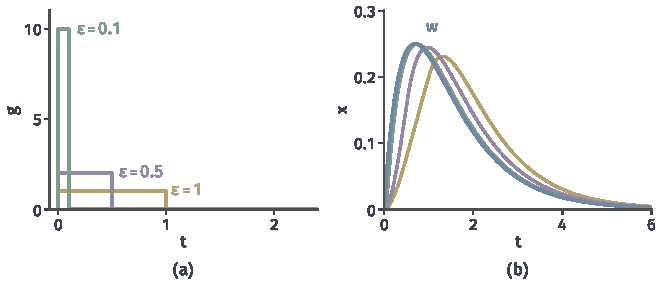
\includegraphics[width=112mm]{figures/06-differential-equations/01-ordinary-differential-equations/matplotlib/lde-pulse-limit/figure.pdf}
  \caption{窄脉冲的响应趋于脉冲响应，方程$\ddot{x}+3\dot{x}+2x=g$，零初值。(a)单位面积的矩形输入，宽度$\varepsilon=1,0.5,0.1$。(b)相同颜色的线是对应的精确响应，蓝线是脉冲响应$w=\mathrm{e}^{-t}-\mathrm{e}^{-2t}$。}
  \label{fig:lde-pulse-limit}
\end{BookInlineFigure}

\paragraph{输入是脉冲的叠加}
叠加原理让这个思想实验变成计算方法。把输入切成许多细长的矩形，每个矩形近似一次脉冲，响应是它们各自响应的总和；矩形变窄时，这个和就成为积分~\eqref{eq:lde-green-solution}。

取$\dot{x}=-x+g$，$g(t)=1+\cos t$，$x(0)=0$，此时$G(t,s)$在$t\geq s$时等于$\mathrm{e}^{-(t-s)}$。直接积分时用到
\[
 \int_0^t\mathrm{e}^{-(t-s)}\cos s\,\mathrm{d}s=\frac{\cos t+\sin t-\mathrm{e}^{-t}}{2},
\]
于是
\[
 x(t)=1+\frac{\cos t+\sin t}{2}-\frac32\mathrm{e}^{-t}.
\]

图~\ref{fig:lde-impulse-superposition}把$[0,6]$切成宽$0.5$的矩形。(b)中每条黄线是一个矩形的响应：输入期间上升，输入结束后按$\mathrm{e}^{-t}$衰减。它们的和（绿线）已经很接近精确解（蓝线），矩形取得更窄时差别还会减小。

\begin{BookInlineFigure}
  \centering
  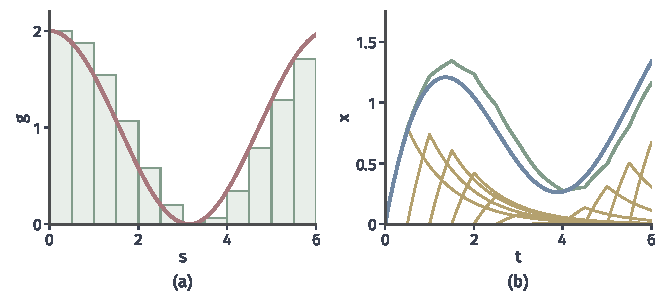
\includegraphics[width=112mm]{figures/06-differential-equations/01-ordinary-differential-equations/matplotlib/lde-impulse-superposition/figure.pdf}
  \caption{输入响应是脉冲响应的叠加，方程$\dot{x}=-x+g$，$x(0)=0$。(a)红线是输入$g=1+\cos s$，绿色矩形是宽$0.5$的分段常值近似，高度取矩形左端的$g$值。(b)黄线是单个矩形输入的响应，绿线是它们的和，蓝线是精确解。}
  \label{fig:lde-impulse-superposition}
\end{BookInlineFigure}

\paragraph{把算子看成下三角矩阵}
把函数看成无限维向量，可以换一个角度理解$\bm{G}$。在等距网格$t_k=t_0+kh$上，式~\eqref{eq:lde-green-solution}近似为一个矩阵乘向量：
\[
 x(t_i)\approx\sum_{j<i}hG(t_i,t_j)g(t_j).
\]
矩阵的第$(i,j)$元是$hG(t_i,t_j)$。第$j$列是在时刻$t_j$敲一下之后的响应序列，第$i$行说明时刻$t_i$的状态怎样加权历史上的输入。

$G(t_i,t_j)$在$j>i$时为零，这个矩阵是下三角的，所以因果性就是下三角结构。图~\ref{fig:lde-green-heatmap}(a)画出$\dot{x}=-x+g$的$G(t,s)$，只有对角线上方有值。类比的限度在于对角线：矩阵元是有限数，而$G$在对角线上的跳变对应着连续问题中$\delta$的位置，它不是任何矩阵元能单独表示的。

同样叫Green函数，边值问题的情形却不同。图~\ref{fig:lde-green-heatmap}(b)是$-\mathrm{d}^2u/\mathrm{d}x^2=f$、$u(0)=u(1)=0$的积分核$\min(x,s)(1-\max(x,s))$，它在对角线两侧都不为零。空间中的边界条件同时从两端约束解，一点的源影响所有位置，没有“先后”可言。这种边值Green函数由第~\ref{chap:elliptic-equations}章介绍。

\begin{BookInlineFigure}
  \centering
  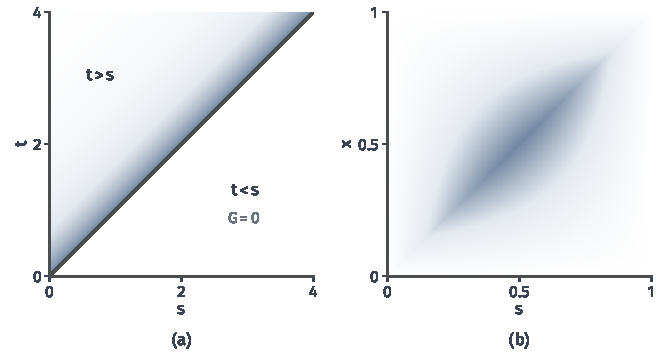
\includegraphics[width=112mm]{figures/06-differential-equations/01-ordinary-differential-equations/matplotlib/lde-green-heatmap/figure.pdf}
  \caption{因果Green函数与边值积分核的对比，颜色越深表示数值越大。(a)$G(t,s)=\mathrm{e}^{-(t-s)}\mathbb{I}_{[s,\infty)}(t)$，深灰线是对角线$t=s$，其下方$G$为零，体现因果性。(b)两点边值问题的核$\min(x,s)(1-\max(x,s))$，对角线两侧都不为零。}
  \label{fig:lde-green-heatmap}
\end{BookInlineFigure}


\section{Laplace变换求解}
\label{sec:lde-laplace}

常系数方程的公式已经齐备，但计算$\mathrm{e}^{t\bm{A}}$和卷积积分有时并不轻松。另一条路线是把求导变成乘法，把初值自动放进代数方程，再把结果翻译回时间域。这条路线要回答三件事：变换何时有定义，初值怎样进入，反过来的翻译是否唯一？

\paragraph{用指数权给函数“称重”}
考虑积分$\int_0^{\infty}\mathrm{e}^{-zt}f(t)\,\mathrm{d}t$。$\mathrm{e}^{-zt}$是一个衰减的权，$z$的实部越大，权衰减得越快，增长的函数也能被压住。图~\ref{fig:lde-laplace-weight}取$f=\mathrm{e}^{t}$：$z=0.5$时乘积仍在增长，$z=1$时是常数，只有$z=2$时乘积衰减，积分收敛。

把$z$取遍一个半平面，就得到一族读数，它们记录了$f$的全部信息。与Fourier变换相比，这里只积分$t\geq0$，并带有衰减权，所以允许指数增长的函数；当$z$在虚轴上时，它就是$f\mathbb{I}_{[0,\infty)}$的Fourier变换。后者的性质可参考\BookChapterRef{chap:fourier-transform}{卷四第14章“Fourier变换”}。

\begin{BookInlineFigure}
  \centering
  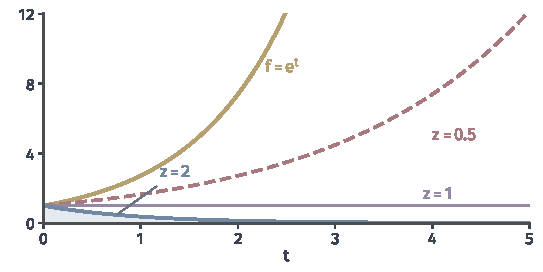
\includegraphics[width=92mm]{figures/06-differential-equations/01-ordinary-differential-equations/matplotlib/lde-laplace-weight/figure.pdf}
  \caption{指数权压住增长。黄线是$f=\mathrm{e}^{t}$，其余曲线是乘积$\mathrm{e}^{-zt}f(t)$：红色虚线$z=0.5$仍增长，紫线$z=1$恒为$1$，蓝线$z=2$衰减，浅蓝是收敛积分的面积$1$。}
  \label{fig:lde-laplace-weight}
\end{BookInlineFigure}

\begin{definition}[单边Laplace变换]
\label{def:lde-laplace}
设$f:[0,\infty)\to\mathbb{C}$在每个有界区间上分段连续（有限个间断点，左右极限都有限），且存在常数$M\geq0$和$c\in\mathbb{R}$使$\lvert f(t)\rvert\leq M\mathrm{e}^{ct}$对所有$t\geq0$成立，就称$f$是\term{指数阶函数}（function of exponential order）。对$\operatorname{Re}z>c$，定义$f$的\term{单边Laplace变换}（unilateral Laplace transform）
\begin{equation}
 \hat{f}(z)=\mathcal{L}[f](z)=\int_0^{\infty}\mathrm{e}^{-zt}f(t)\,\mathrm{d}t.
 \label{eq:lde-laplace}
\end{equation}
\end{definition}

记$\sigma=\operatorname{Re}z$。$\sigma>c$时被积函数的模不超过$M\mathrm{e}^{-(\sigma-c)t}$，所以积分绝对收敛，并且$\lvert\hat{f}(z)\rvert\leq M/(\sigma-c)$。不是每个函数都有变换：$\mathrm{e}^{t^2}$增长得比任何指数都快，对任何$z$积分都发散。

\paragraph{常用变换对}
直接积分可得$\mathcal{L}[\mathrm{e}^{at}](z)=1/(z-a)$，收敛条件是$\operatorname{Re}z>\operatorname{Re}a$。令$a$取$\pm\mathrm{i}\beta$再线性组合，得到正弦和余弦；对$a$逐次求导，得到$t^k\mathrm{e}^{at}$。表~\ref{tab:lde-laplace-pairs}列出本节用到的结果。

\begin{BookInlineTable}
  \centering
  \caption{常用的单边Laplace变换对，$k$为非负整数，$a\in\mathbb{C}$，$\beta,\tau$为实数，$\tau\geq0$。}
  \label{tab:lde-laplace-pairs}
  \begin{tabular}{lll}
    \toprule
    $f(t)$ & $\hat{f}(z)$ & 收敛范围\\
    \midrule
    $\mathrm{e}^{at}$ & $1/(z-a)$ & $\operatorname{Re}z>\operatorname{Re}a$\\
    $t^k\mathrm{e}^{at}$ & $k!/(z-a)^{k+1}$ & $\operatorname{Re}z>\operatorname{Re}a$\\
    $\cos\beta t$ & $z/(z^2+\beta^2)$ & $\operatorname{Re}z>0$\\
    $\sin\beta t$ & $\beta/(z^2+\beta^2)$ & $\operatorname{Re}z>0$\\
    $\mathrm{e}^{at}f(t)$ & $\hat{f}(z-a)$ & $\operatorname{Re}z>c+\operatorname{Re}a$\\
    $f(t-\tau)\mathbb{I}_{[\tau,\infty)}(t)$ & $\mathrm{e}^{-\tau z}\hat{f}(z)$ & $\operatorname{Re}z>c$\\
    \bottomrule
  \end{tabular}
\end{BookInlineTable}

\paragraph{导数公式：初值从这里进入}
方程能被化成代数式，靠的是下面的公式。它也说明了连续性为什么不能省略。

\begin{theorem}[导数的Laplace变换]
\label{thm:lde-laplace-derivative}
设$f$在$[0,\infty)$上连续，分段连续可微，$\dot{f}$是指数阶函数，$\lvert\dot{f}(t)\rvert\leq M\mathrm{e}^{ct}$，其中$c>0$。则$f$也是指数阶函数，并且对$\operatorname{Re}z>c$，
\begin{equation}
 \mathcal{L}[\dot{f}](z)=z\hat{f}(z)-f(0).
 \label{eq:lde-laplace-derivative}
\end{equation}
\end{theorem}

\begin{proof}
由$f(t)=f(0)+\int_0^t\dot{f}$，得到
\[
 \lvert f(t)\rvert\leq\lvert f(0)\rvert+\frac{M}{c}\mathrm{e}^{ct},
\]
所以$f$是指数阶函数。

设$\dot{f}$的间断点为$t_1<t_2<\cdots$。在每一段上分部积分，并把$[0,T]$上的各段相加。$f$连续，所以内部接缝处的边界项两两抵消，只剩两端：
\[
 \int_0^T\mathrm{e}^{-zt}\dot{f}(t)\,\mathrm{d}t=\mathrm{e}^{-zT}f(T)-f(0)+z\int_0^T\mathrm{e}^{-zt}f(t)\,\mathrm{d}t.
\]
$\operatorname{Re}z>c$时，$\lvert\mathrm{e}^{-zT}f(T)\rvert\to0$。令$T\to\infty$就得到结论。
\end{proof}

连续性用在边界项的抵消上。若$f$有跳变，比如$f=\mathbb{I}_{[1,\infty)}$，则$\dot{f}$几乎处处为零，$\mathcal{L}[\dot{f}]=0$；而$z\hat{f}(z)-f(0)=\mathrm{e}^{-z}\neq0$，差额恰好是跳变项。

把公式用两次，得到二阶导数的变换：
\begin{equation}
 \mathcal{L}[\ddot{f}](z)=z^2\hat{f}(z)-zf(0)-\dot{f}(0).
 \label{eq:lde-laplace-second}
\end{equation}
这里要求$f$和$\dot{f}$连续。初值以多项式的形式出现在右端，所以不需要先求通解、再定常数。

\paragraph{卷积与唯一性}
式~\eqref{eq:lde-convolution-response}的卷积也有简单的像。对$[0,\infty)$上的函数，记$(f*g)(t)=\int_0^tf(t-s)g(s)\,\mathrm{d}s$。

\begin{theorem}[卷积定理]
\label{thm:lde-laplace-convolution}
设$f,g$是指数阶函数，相应的增长指数都不超过$c$。则$f*g$连续并且是指数阶函数，对$\operatorname{Re}z>c$有
\begin{equation}
 \mathcal{L}[f*g](z)=\hat{f}(z)\hat{g}(z).
 \label{eq:lde-laplace-convolution}
\end{equation}
\end{theorem}

\begin{proof}
由$\lvert f\rvert\leq M_1\mathrm{e}^{ct}$和$\lvert g\rvert\leq M_2\mathrm{e}^{ct}$，得$\lvert(f*g)(t)\rvert\leq M_1M_2t\mathrm{e}^{ct}$，它不超过常数乘$\mathrm{e}^{c't}$（任取$c'>c$）。连续性可由控制收敛定理得到。

设$\sigma=\operatorname{Re}z>c$。二重积分
\[
 \int_0^{\infty}\!\!\int_0^t\lvert\mathrm{e}^{-zt}f(t-s)g(s)\rvert\,\mathrm{d}s\,\mathrm{d}t\leq\frac{M_1M_2}{(\sigma-c)^2}
\]
有限：非负被积函数可以先对$t$积分，令$r=t-s$就得到右端的界。所以可用Fubini定理交换积分次序，同样令$r=t-s$：
\[
 \int_0^{\infty}\!\!\int_s^{\infty}\mathrm{e}^{-zt}f(t-s)g(s)\,\mathrm{d}t\,\mathrm{d}s=\int_0^{\infty}\mathrm{e}^{-zs}g(s)\,\mathrm{d}s\int_0^{\infty}\mathrm{e}^{-zr}f(r)\,\mathrm{d}r.
\]
右端正是$\hat{f}(z)\hat{g}(z)$。
\end{proof}

从像函数翻译回时间函数，要先知道翻译是唯一的。函数在个别点上的取值不影响积分，所以唯一性只能精确到这些点。

\begin{theorem}[Laplace变换的唯一性]
\label{thm:lde-laplace-uniqueness}
设$f_1,f_2$是指数阶函数，并且存在实数$b$，使$\hat{f}_1(z)=\hat{f}_2(z)$对所有$z>b$的实数成立。则在$f_1$和$f_2$的每个公共连续点上都有$f_1=f_2$。
\end{theorem}

\begin{proof}
令$f=f_1-f_2$，取整数$k>\max(b,c)$，其中$c$使$\lvert f\rvert\leq M\mathrm{e}^{ct}$成立。作代换$u=\mathrm{e}^{-t}$，令$\varphi(u)=u^{k}f(-\ln u)$，$u\in(0,1]$。由$\lvert\varphi(u)\rvert\leq Mu^{k-c}$，$\varphi$在$(0,1]$上有界。对$m=0,1,2,\ldots$，
\[
 0=\hat{f}(k+1+m)=\int_0^{\infty}\mathrm{e}^{-(k+1+m)t}f(t)\,\mathrm{d}t=\int_0^1u^{m}\varphi(u)\,\mathrm{d}u.
\]

所以$\varphi$与每个多项式的乘积积分为零。给定$\eta>0$，取$[0,1]$上的连续函数$\psi$使$\int_0^1\lvert\varphi-\psi\rvert\leq\eta$，由Weierstrass逼近定理再取多项式$q$，使$\sup\lvert\psi-q\rvert\leq\eta$，记$B=\sup\lvert\varphi\rvert$。于是
\[
 \int_0^1\lvert\varphi\rvert^2=\int_0^1\bar{\varphi}(\varphi-\psi)+\int_0^1\bar{\varphi}(\psi-q)+\int_0^1\bar{\varphi}q.
\]
最后一项是$\int_0^1\varphi\bar{q}$的共轭，等于零，前两项各不超过$B\eta$，所以$\int_0^1\lvert\varphi\rvert^2\leq2B\eta$。$\eta$任意，得$\int_0^1\lvert\varphi\rvert^2=0$。分段连续函数平方积分为零，就在其每个连续点上为零。
\end{proof}

证明中的多项式逼近定理可参考\BookChapterRef{chap:function-approximation}{卷四第20章“函数逼近”}。定理告诉我们，只要在表中找到一个时间函数，它的变换等于所求的像函数，这个函数就是答案。一般的反演积分公式需要复变函数，本节的有理函数都用部分分式和查表处理，不必用到它。

\paragraph{求解的三步}
常系数方程的求解分三步。第一步，对方程两边作变换，用式~\eqref{eq:lde-laplace-derivative}和式~\eqref{eq:lde-laplace-second}代入初值，得到关于$\hat{x}$的代数方程。第二步，解出$\hat{x}$，它通常是有理函数。第三步，把$\hat{x}$拆成部分分式，查表得到$x$，再代回原问题检验。

\begin{example}[带初值的阶跃响应]
\label{ex:lde-laplace-step}
求解例~\ref{ex:lde-step-response}的问题$\ddot{x}+3\dot{x}+2x=1$，$x(0)=1$，$\dot{x}(0)=0$。作变换，右端的像是$1/z$，左端由式~\eqref{eq:lde-laplace-second}和式~\eqref{eq:lde-laplace-derivative}得到
\[
 (z^2\hat{x}-z)+3(z\hat{x}-1)+2\hat{x}=\frac1z.
\]
合并含$\hat{x}$的项，并解出
\[
 \hat{x}(z)=\frac{z^2+3z+1}{z(z+1)(z+2)}.
\]
三个极点都是单极点。对单极点$p$，部分分式的系数是把因子$(z-p)$约去后在$z=p$处取值，于是
\[
 \hat{x}(z)=\frac{1/2}{z}+\frac{1}{z+1}-\frac{1/2}{z+2}.
\]
由表~\ref{tab:lde-laplace-pairs}，
\[
 x(t)=\frac12+\mathrm{e}^{-t}-\frac12\mathrm{e}^{-2t},\qquad t\geq0.
\]
这与例~\ref{ex:lde-step-response}的结果一致，那里已经代回方程检验过。最右边的极点是$0$，所以像函数在$\operatorname{Re}z>0$上收敛。
\end{example}

收敛范围与极点的位置直接相关：解的增长指数由最右边的极点决定，收敛半平面从那里开始，图~\ref{fig:lde-laplace-region}给出三个例子。极点的虚部对应振荡，重数对应多项式因子，这与第~\ref{sec:lde-constant}节的特征根完全对应。

\begin{BookInlineFigure}
  \centering
  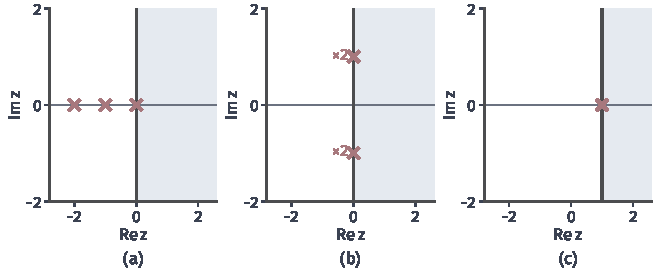
\includegraphics[width=112mm]{figures/06-differential-equations/01-ordinary-differential-equations/matplotlib/lde-laplace-region/figure.pdf}
  \caption{像函数的极点（红叉）与收敛半平面（浅蓝，边界为深灰竖线）。(a)例~\ref{ex:lde-laplace-step}的极点$0,-1,-2$。(b)共振例的二重极点$\pm\mathrm{i}$。(c)$\mathrm{e}^{t}$的极点$1$，收敛范围是$\operatorname{Re}z>1$。}
  \label{fig:lde-laplace-region}
\end{BookInlineFigure}

\paragraph{复极点、重极点与共振}
复极点常用配方处理。对$\ddot{x}+2\dot{x}+5x=0$，$x(0)=1$，$\dot{x}(0)=0$，同样作变换解出$\hat{x}=(z+2)/(z^2+2z+5)$。分母配方为$(z+1)^2+4$，分子写成$(z+1)+1$，于是
\[
 \hat{x}(z)=\frac{z+1}{(z+1)^2+4}+\frac12\cdot\frac{2}{(z+1)^2+4}.
\]
用表中的平移规则和正弦、余弦的变换，得到$x(t)=\mathrm{e}^{-t}(\cos2t+\frac12\sin2t)$，与第~\ref{sec:lde-high-order}节的结果相同。

重极点对应输入与齐次模式的配合。取$\ddot{x}+2\dot{x}+x=\mathrm{e}^{-t}$，零初值。特征根$-1$是二重的，输入又含有同一模式，像函数的极点升到三重：
\[
 \hat{x}(z)=\frac{1}{(z+1)^3}.
\]
由表得$x(t)=\frac12t^2\mathrm{e}^{-t}$。代回检验，
\[
 \dot{x}=\Bigl(t-\frac{t^2}{2}\Bigr)\mathrm{e}^{-t},\qquad
 \ddot{x}=\Bigl(1-2t+\frac{t^2}{2}\Bigr)\mathrm{e}^{-t}.
\]
于是$\ddot{x}+2\dot{x}+x=\mathrm{e}^{-t}$，且$x(0)=\dot{x}(0)=0$。

卷积定理把这一节和常数变易公式联系起来。式~\eqref{eq:lde-forced-oscillator}取$\omega_0=\omega=1$，作变换得
\[
 \hat{x}(z)=\frac{z}{(z^2+1)^2}=\frac{1}{z^2+1}\cdot\frac{z}{z^2+1}.
\]
两个因子分别是$\sin t$和$\cos t$的像，乘积对应卷积$\int_0^t\sin(t-s)\cos s\,\mathrm{d}s$，这正是积分~\eqref{eq:lde-forced-integral}。另一方面，对表中$\mathcal{L}[\sin t](z)=1/(z^2+1)$关于$z$求导，可得$\mathcal{L}[t\sin t](z)=2z/(z^2+1)^2$，于是$x(t)=\tfrac12t\sin t$，与式~\eqref{eq:lde-resonance}相同。二重极点$\pm\mathrm{i}$就是频率上的共振。

\paragraph{分段输入}
延迟规则让分段输入也能一次写出。取$\dot{x}=-x+g$，$x(0)=0$，$g$在$[0,1)$上为$1$，其余时刻为$0$。写$g=\mathbb{I}_{[0,\infty)}-\mathbb{I}_{[1,\infty)}$，得$\hat{g}=(1-\mathrm{e}^{-z})/z$，于是
\[
 \hat{x}(z)=(1-\mathrm{e}^{-z})\Bigl(\frac1z-\frac{1}{z+1}\Bigr).
\]
$1/z-1/(z+1)$对应$1-\mathrm{e}^{-t}$，因子$\mathrm{e}^{-z}$把它延迟$1$，所以
\[
 x(t)=1-\mathrm{e}^{-t}-\bigl(1-\mathrm{e}^{-(t-1)}\bigr)\mathbb{I}_{[1,\infty)}(t).
\]

分段直接解可以验证。在$[0,1)$上是$1-\mathrm{e}^{-t}$；$t\geq1$时方程齐次，从$x(1)=1-\mathrm{e}^{-1}$出发，得$(\mathrm{e}-1)\mathrm{e}^{-t}$。上式在$t\geq1$时化简后也是$(\mathrm{e}-1)\mathrm{e}^{-t}$。$g$在$t=1$跳变，$x$连续但有折角，这是分段输入的绝对连续解。

\paragraph{向量系统与预解矩阵}
对向量系统$\dot{\bm{x}}=\bm{A}\bm{x}+\bm{g}$逐分量作变换，由式~\eqref{eq:lde-laplace-derivative}得到
\[
 (z\bm{I}-\bm{A})\hat{\bm{x}}(z)=\bm{x}_0+\hat{\bm{g}}(z).
\]
矩阵$(z\bm{I}-\bm{A})^{-1}$称为\term{预解矩阵}（resolvent matrix），它把微分方程的传播变成了代数求逆。

\begin{theorem}[矩阵指数的变换]
\label{thm:lde-resolvent}
设$\bm{A}$的特征值实部的最大值为$\gamma$。则对$\operatorname{Re}z>\gamma$，
\begin{equation}
 \mathcal{L}[\mathrm{e}^{t\bm{A}}](z)=\int_0^{\infty}\mathrm{e}^{-zt}\mathrm{e}^{t\bm{A}}\,\mathrm{d}t=(z\bm{I}-\bm{A})^{-1}.
 \label{eq:lde-resolvent}
\end{equation}
于是向量系统的像函数是
\begin{equation}
 \hat{\bm{x}}(z)=(z\bm{I}-\bm{A})^{-1}\bigl(\bm{x}_0+\hat{\bm{g}}(z)\bigr),
 \label{eq:lde-vector-transform}
\end{equation}
它对应时间域的公式~\eqref{eq:lde-duhamel-constant}。
\end{theorem}

\begin{proof}
由定理~\ref{thm:lde-exponential-shape}，$\mathrm{e}^{t\bm{A}}$的元素是$t^j\mathrm{e}^{\lambda t}$的组合，所以对任何$c>\gamma$，存在$C$使下式成立：
\[
 \lVert\mathrm{e}^{t\bm{A}}\rVert_2\leq C\mathrm{e}^{ct}.
\]
取$c$介于$\gamma$与$\operatorname{Re}z$之间，积分绝对收敛。

由定理~\ref{thm:lde-matexp-properties}的(2)，
\[
 \frac{\mathrm{d}}{\mathrm{d}t}\bigl(\mathrm{e}^{-zt}\mathrm{e}^{t\bm{A}}\bigr)=\mathrm{e}^{-zt}\mathrm{e}^{t\bm{A}}(\bm{A}-z\bm{I}).
\]
从$0$积分到$\infty$，左端等于$-\bm{I}$，因为$t\to\infty$时$\mathrm{e}^{-zt}\mathrm{e}^{t\bm{A}}\to\bm{0}$。两边右乘$-(z\bm{I}-\bm{A})^{-1}$；这里$\operatorname{Re}z>\gamma$，$z$不是特征值，矩阵可逆。
\end{proof}

对例~\ref{ex:lde-running-system}的矩阵，
\[
 (z\bm{I}-\bm{A})^{-1}=\frac{1}{(z+1)(z+2)}\begin{bmatrix}z+3&1\\-2&z\end{bmatrix}.
\]
部分分式给出$(1,1)$元$(z+3)/((z+1)(z+2))=2/(z+1)-1/(z+2)$，对应$2\mathrm{e}^{-t}-\mathrm{e}^{-2t}$。$(1,2)$元$1/((z+1)(z+2))=1/(z+1)-1/(z+2)$，对应脉冲响应$w=\mathrm{e}^{-t}-\mathrm{e}^{-2t}$。式~\eqref{eq:lde-resolvent}也说明，因果Green函数$\bm{H}$的变换就是预解矩阵。

\paragraph{方法的边界}
Laplace变换依赖两点：系数是常数，输入是指数阶函数。乘以$t$在变换后变成对$z$求导，所以系数含$t$的方程变成关于$\hat{x}$的微分方程，一般并不比原方程容易。此外，部分分式需要分母的全部根，高阶情形要靠数值计算。这些限制下，第~\ref{sec:lde-time-varying}节的状态转移矩阵和第~\ref{chap:ode-numerical-methods}章的数值方法是必要的。


\section{本章小结}
\label{sec:lde-summary}

线性方程把初始状态和外部输入线性地映成响应，本章的所有公式都是这个线性映射的不同写法。标量方程用积分因子得到显式解，公式在系数连续的整个区间上成立；系数只可积时，同一公式在积分形式下仍然成立，解是绝对连续函数。

常系数系统的传播是矩阵指数，它满足齐次方程和单位初值。对角化把系统分解成独立的模式，复特征值对应旋转和伸缩，三角形式让系统逐行回代。特征根决定解的成分，但只看特征值是不够的：相同的特征值可以有不同数量的特征向量，广义特征向量带来$t$的多项式因子和有限时间的放大。高阶标量方程经状态降阶化为友矩阵系统，重根必定带来多项式因子。

时变系统的传播是状态转移矩阵。它依赖初始时刻和终止时刻，满足复合关系，由基本解矩阵算出。各时刻的系数不可交换时，时间次序不能丢弃，$\exp\int\bm{A}$不是传播；所有时刻的系数都可交换时，这个简化才成立。

非齐次方程的解等于零输入响应加零状态响应，常数变易公式把输入看成不断注入、并继续传播的状态增量。共振来自输入与齐次模式的配合，它与Jordan链上的多项式因子是同一机制。因果Green函数是单位脉冲的响应，它在输入发生之前为零，离散以后是下三角矩阵。Laplace变换把常系数方程化为代数方程，初值自动进入，极点的位置和重数对应解的增长、振荡和多项式因子。

表~\ref{tab:lde-methods}对照了这些方法的适用范围。

\begin{BookInlineTable}
  \centering
  \caption{线性初值问题的四种工具。}
  \label{tab:lde-methods}
  \begin{tabular}{lll}
    \toprule
    方法 & 系数 & 输入\\
    \midrule
    积分因子 & 标量，连续或局部可积 & 连续或局部可积\\
    矩阵指数 & 常矩阵 & 连续或局部可积\\
    状态转移矩阵 & 连续或局部可积的矩阵 & 连续或局部可积\\
    Laplace变换 & 常系数 & 指数阶、分段连续\\
    \bottomrule
  \end{tabular}
\end{BookInlineTable}

非线性方程在一条已知轨迹附近的小扰动，满足的正是线性时变方程，所以状态转移矩阵和常数变易公式会在第~\ref{chap:ode-sensitivity}章重新出现。本章的结论都是有限时间上的显式刻画；响应在无穷长时间内是否稳定、输入按频率怎样被放大，以及怎样设计反馈来改变传播，都不是这里的问题。


\chapter{解的存在性}
\label{chap:ode-existence-continuation}

先看三个写法同样简单的初值问题，它们都是一个实数状态的方程。第一个是$\dot x=x^2$，$x(0)=1$，公式$x(t)=1/(1-t)$在$t=1$之前有效，到$t=1$时状态冲向无穷。第二个是$\dot x=2\sqrt{\lvert x\rvert}$，$x(0)=0$，曲线$x\equiv0$和$x=t^2$都满足它，初值没有确定唯一的未来。第三个的右端在$x\geq0$时取$-1$，在$x<0$时取$1$，从$x(0)=0$出发根本找不到解。

这三个方程的右端都能在一行之内写完，可见“写得出方程”并不等于“有一条确定的解曲线”。没有解析公式的方程也需要回答这些问题：解是否存在，是否只有一条，能走多远。这些回答决定了后面的敏感性分析和数值计算是否在谈论一个确定的对象。

本章先在连续右端下证明局部存在，它依赖有限维空间的紧性，只保证有解。给右端加上状态方向的Lipschitz条件之后，积分方程在一段短时间上成为压缩映射的不动点问题，局部存在和唯一性同时得到，并给出可计算的迭代。局部解沿唯一性拼接成最大解，解走不下去只有离开定义域中每个紧集这一种方式，至多线性增长的右端排除了这种情形。

最后放宽两个方向。时间方向上，右端只需可测，解换成绝对连续曲线，所需的条件和结论都要相应调整。空间方向上，状态可以在流形上，局部用坐标解方程，靠唯一性把各张图上的解接成同一条曲线。

\section{局部存在}
\label{sec:odeex-local-existence}

给定一个开集$\bm{D}\subseteq\mathbb{R}\times\mathbb{R}^{n}$、一个连续映射$\bm{f}:\bm{D}\to\mathbb{R}^{n}$和一点$(t_0,\bm{x}_0)\in\bm{D}$，我们要找区间$I\ni t_0$上的连续可微曲线$\bm{x}$，使$(t,\bm{x}(t))\in\bm{D}$，并且
\begin{equation}
 \dot{\bm{x}}(t)=\bm{f}(t,\bm{x}(t)),\quad t\in I,\qquad \bm{x}(t_0)=\bm{x}_0.
 \label{eq:odeex-ivp}
\end{equation}
这样的曲线称为经典解。右端连续时，由第~\ref{chap:ordinary-differential-equations}章的讨论，式~\eqref{eq:odeex-ivp}等价于连续曲线满足积分方程
\begin{equation}
 \bm{x}(t)=\bm{x}_0+\int_{t_0}^{t}\bm{f}(s,\bm{x}(s))\,\mathrm{d}s,\quad t\in I.
 \label{eq:odeex-integral}
\end{equation}
积分号里的被积函数连续，所以满足式~\eqref{eq:odeex-integral}的连续曲线自动连续可微，并且在$t_0$处取值$\bm{x}_0$。

只知道右端连续，能否断定这样的曲线至少存在一小段？图像上的问题是：平面每一点都标着一个小箭头，从起点出发能不能画一条处处与箭头相切的曲线。最自然的办法是顺着箭头走一小步，停下来看新位置的箭头，再走一小步。

\paragraph{顺着方向场走折线}
取步长$h>0$，时间网格$t_k=t_0+kh$。从$\bm{x}^{(0)}=\bm{x}_0$出发，每一步沿当前箭头走直线：
\begin{equation}
 \bm{x}^{(k+1)}=\bm{x}^{(k)}+h\,\bm{f}(t_k,\bm{x}^{(k)}).
 \label{eq:odeex-euler-node}
\end{equation}
把相邻的点用线段连起来，得到一条折线，称为\term{Euler折线}（Euler polygon）。第~\ref{chap:ode-numerical-methods}章会把它当作数值方法研究误差，这里只用它来证明解的存在。

用$\dot x=x^2$，$x(0)=1$在$[0,1/4]$上试算。取$N=2$步，$h=1/8$，两步的结果分别是
\[
 x^{(1)}=1+\frac18\cdot1^2=1.125,\qquad x^{(2)}=1.125+\frac18\cdot1.125^2\approx1.2832.
\]
真解在$t=1/4$处等于$4/3\approx1.3333$。取$N=4$和$N=8$，折线的终点依次为
\[
 1.3053,\qquad 1.3184.
\]
图~\ref{fig:odeex-euler-refinement}画出了这些折线。每条折线都在真解下方，因为$x^2$沿解递增，折线在每段上采用的是该段开始时较小的斜率；步长减半时，折线向真解靠拢。

\begin{BookInlineFigure}
  \centering
  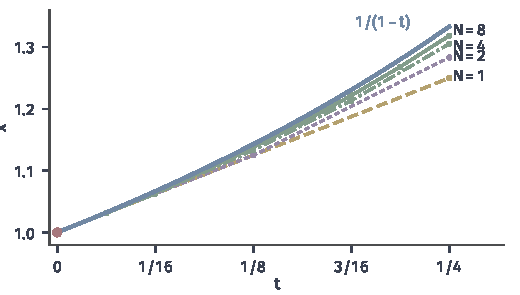
\includegraphics[width=88mm]{figures/06-differential-equations/01-ordinary-differential-equations/matplotlib/odeex-euler-refinement/figure.pdf}
  \caption{初值问题$\dot x=x^2$，$x(0)=1$在$[0,1/4]$上的Euler折线。蓝色粗线是真解$1/(1-t)$，其余折线的步数$N$分别为$1,2,4,8$，红点是初值。步数增加时折线向真解靠拢。}
  \label{fig:odeex-euler-refinement}
\end{BookInlineFigure}

这里的真解是预先知道的。对一般的连续右端，没有真解可作比较，也无从知道折线列是否收敛。我们手里只有折线本身的信息，要从中取出一条极限曲线，就要先把折线关在一个固定的范围内。

\paragraph{盒子与时间窗}
先选一个以初值为中心的盒子。取$a,b>0$足够小，记
\begin{equation}
 \bm{B}_b=\{\bm{x}\in\mathbb{R}^{n}:\lVert\bm{x}-\bm{x}_0\rVert_2\leq b\},\qquad
 \bm{Q}=[t_0-a,t_0+a]\times\bm{B}_b,
 \label{eq:odeex-box}
\end{equation}
使$\bm{Q}\subseteq\bm{D}$。$\bm{D}$是开集，这总能做到。$\bm{Q}$是紧集，连续函数$\lVert\bm{f}\rVert_2$在其上有最大值，取$M>0$使$\lVert\bm{f}\rVert_2\leq M$在$\bm{Q}$上成立。

$M$是盒子内箭头的最大速度。一条曲线只要还在盒子内，到初值的距离就至多以速率$M$增长，所以它被限制在以$(t_0,\bm{x}_0)$为顶点、斜率$\pm M$的锥内。它可能从盒子的上下壁离开，这要花至少$b/M$的时间；也可能走到盒子的左右壁，这要花时间$a$。于是在时间窗
\begin{equation}
 \delta=\min\Bigl\{a,\frac{b}{M}\Bigr\}
 \label{eq:odeex-peano-window}
\end{equation}
内，曲线不会离开盒子。

图~\ref{fig:odeex-existence-box}用前面的方程演示这一计算。取$b=1$，状态范围是$[0,2]$，其上$x^2\leq4$，所以$M=4$。图(a)中$a=1/2$，$\delta=\min\{1/2,1/4\}=1/4$，锥先碰到上壁。图(b)中$a=3/20$，$\delta=3/20$，锥先碰到右壁。真解实际能走到$t=1$，时间窗只是一个保守的保证。

\begin{BookInlineFigure}
  \centering
  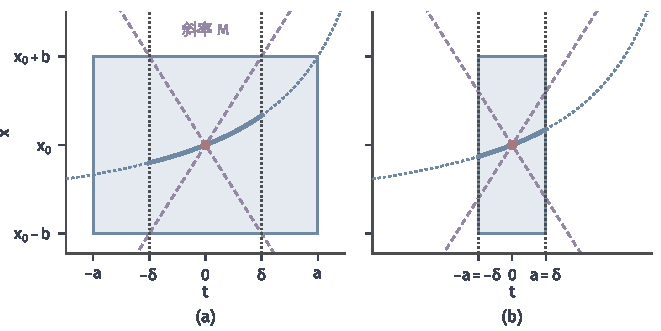
\includegraphics[width=112mm]{figures/06-differential-equations/01-ordinary-differential-equations/matplotlib/odeex-existence-box/figure.pdf}
  \caption{盒子与时间窗。浅蓝矩形是$\bm{Q}$，这里$x_0=1$，$b=1$，紫色虚线是斜率$\pm M=\pm4$的锥，蓝色粗线是真解在时间窗内的部分，蓝色点线是它在窗外的延续。(a)$a=1/2$，$\delta=b/M=1/4$，由状态范围决定。(b)$a=3/20$，$\delta=a$，由时间范围决定。}
  \label{fig:odeex-existence-box}
\end{BookInlineFigure}

\paragraph{Peano存在定理}
盒子内的折线有共同的速度上限，这件事足以让我们从折线列中抽出一条收敛的曲线。结论是下面的\term{Peano存在定理}（Peano existence theorem）。

\begin{theorem}[Peano存在定理]
\label{thm:odeex-peano}
设$\bm{D}\subseteq\mathbb{R}\times\mathbb{R}^{n}$是开集，$\bm{f}:\bm{D}\to\mathbb{R}^{n}$连续，$(t_0,\bm{x}_0)\in\bm{D}$。按式~\eqref{eq:odeex-box}取$\bm{Q}\subseteq\bm{D}$，取$M>0$使$\lVert\bm{f}\rVert_2\leq M$在$\bm{Q}$上成立，再按式~\eqref{eq:odeex-peano-window}确定$\delta$。则初值问题~\eqref{eq:odeex-ivp}在$[t_0-\delta,t_0+\delta]$上至少有一个经典解，解的取值都在$\bm{B}_b$中。
\end{theorem}

证明分三步：折线留在盒子内，折线列有一致收敛的子列，子列的极限满足积分方程。第一步用$\bm{f}$的有界性，第二步用有限维的紧性，第三步用$\bm{f}$的连续性。

\begin{proof}
先在$I^+=[t_0,t_0+\delta]$上构造解。对正整数$N$，取$h=\delta/N$，按式~\eqref{eq:odeex-euler-node}得到节点$\bm{x}^{(0)},\ldots,\bm{x}^{(N)}$，记相应的折线为$\bm{y}_N$，即对$t\in[t_k,t_{k+1}]$，
\[
 \bm{y}_N(t)=\bm{x}^{(k)}+(t-t_k)\,\bm{f}(t_k,\bm{x}^{(k)}).
\]

\emph{折线留在盒子内。}对$k$归纳证明$\lVert\bm{x}^{(k)}-\bm{x}_0\rVert_2\leq Mkh$。$k=0$时成立。若对$k<N$成立，则$Mkh\leq M\delta\leq b$，$(t_k,\bm{x}^{(k)})\in\bm{Q}$，所以$\lVert\bm{f}(t_k,\bm{x}^{(k)})\rVert_2\leq M$，于是
\[
 \lVert\bm{x}^{(k+1)}-\bm{x}_0\rVert_2\leq\lVert\bm{x}^{(k)}-\bm{x}_0\rVert_2+hM\leq M(k+1)h.
\]
因此所有节点都在球$\bm{B}_b$中。球是凸集，线段也在其中，折线的取值全在$\bm{B}_b$内，节点上的速度都不超过$M$。

\emph{抽取收敛子列。}折线每段的斜率范数不超过$M$，所以对$s,t\in I^+$，
\[
 \lVert\bm{y}_N(t)-\bm{y}_N(s)\rVert_2\leq M\lvert t-s\rvert.
\]
这说明$\{\bm{y}_N\}$的各分量等度连续，而它们又一致有界（取值在$\bm{B}_b$中）。紧区间上一致有界且等度连续的实函数族，由Arzelà--Ascoli判据在一致距离下相对紧，每个序列都有一致收敛的子列，可参考\BookChapterRef{chap:function-class-covers}{卷四第13章“函数类的有限覆盖”}。对$n$个分量依次抽取子列，得到$\bm{y}_{N_j}$一致收敛到连续曲线$\bm{x}:I^+\to\bm{B}_b$。

\emph{极限满足积分方程。}对$s\in[t_k,t_{k+1})$，记$\sigma_N(s)=t_k$，它是$s$所在网格段的左端点。折线分段线性，由其构造，
\[
 \bm{y}_N(t)=\bm{x}_0+\int_{t_0}^{t}\bm{f}\bigl(\sigma_N(s),\bm{y}_N(\sigma_N(s))\bigr)\,\mathrm{d}s.
\]
$\bm{f}$在紧集$\bm{Q}$上一致连续。任取$\varepsilon>0$，存在$\eta>0$，使$\bm{Q}$中两点的时间差与状态距离之和小于$\eta$时，$\bm{f}$值之差的范数小于$\varepsilon$。

比较被积函数在两点的取值：时间差是$s-\sigma_N(s)\leq h$，状态差由三角不等式与斜率上限满足
\[
 \lVert\bm{y}_N(\sigma_N(s))-\bm{x}(s)\rVert_2\leq Mh+\lVert\bm{y}_N-\bm{x}\rVert_{\infty},
\]
这里$\lVert\cdot\rVert_{\infty}$是$I^+$上的一致范数。沿子列$N=N_j$，$h\to0$，$\lVert\bm{y}_N-\bm{x}\rVert_{\infty}\to0$，所以当$j$足够大时，两点距离之和小于$\eta$，对所有$s$都有被积函数之差小于$\varepsilon$。

积分后得到，对$t\in I^+$，
\[
 \Bigl\lVert\int_{t_0}^{t}\bm{f}\bigl(\sigma_N(s),\bm{y}_N(\sigma_N(s))\bigr)\,\mathrm{d}s
 -\int_{t_0}^{t}\bm{f}(s,\bm{x}(s))\,\mathrm{d}s\Bigr\rVert_2\leq\varepsilon\delta.
\]
令$j\to\infty$，$\bm{x}$在$I^+$上满足积分方程~\eqref{eq:odeex-integral}。

\emph{向左延伸。}令$\tilde{\bm{x}}(s)=\bm{x}(2t_0-s)$，方程变成
\[
 \frac{\mathrm{d}\tilde{\bm{x}}}{\mathrm{d}s}=-\bm{f}(2t_0-s,\tilde{\bm{x}}),
\]
其右端满足同样的条件和同样的上界。对它应用前面的结论，得到$[t_0-\delta,t_0]$上的解。两段在$t_0$处都取$\bm{x}_0$，合起来在整个区间上满足式~\eqref{eq:odeex-integral}，因而是经典解。
\end{proof}

\paragraph{连续性在哪里起作用}
证明第三步用连续性把折线所用的箭头换成极限曲线上的箭头。若右端不连续，这一步会失败，解也可能真的不存在。取
\[
 f(x)=\begin{cases}-1,&x\geq0,\\ 1,&x<0,\end{cases}\qquad x(0)=0.
\]
箭头从两侧都指向$x=0$，图~\ref{fig:odeex-discontinuous-chatter}(a)中从$x=\pm1$出发的解都在$t=1$到达零线，到达之后就停在那里。

假设有解从$x(0)=0$出发。若解在某段时间内为正，这段时间的左端点处解为零，而解在段内以速度$-1$下降，不可能从$0$变成正数；同理解不能在某段时间内为负。于是解只能恒为零，而$\dot x=0$不等于$f(0)=-1$，矛盾。

Euler折线看到的是什么？在图~\ref{fig:odeex-discontinuous-chatter}(b)中，它在$0$与$-h$之间来回跳动，当$h\to0$时一致收敛到$x\equiv0$。折线列本身有极限，但折线所用的斜率在$\pm1$之间振荡，平均为$0$，而$f(0)=-1$。极限曲线不满足方程，正是因为第三步的“被积函数收敛”不成立。

\begin{BookInlineFigure}
  \centering
  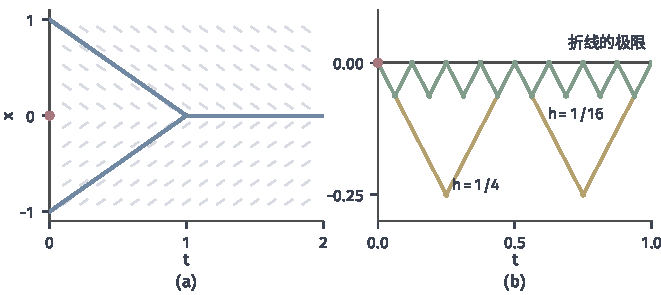
\includegraphics[width=112mm]{figures/06-differential-equations/01-ordinary-differential-equations/matplotlib/odeex-discontinuous-chatter/figure.pdf}
  \caption{右端不连续时存在性失败。$f(x)=-1$（$x\geq0$），$f(x)=1$（$x<0$）。(a)短线是方向场，蓝线是从$x=\pm1$出发的解，到$t=1$时汇入零线后停止延伸，红点是无解的初值$(0,0)$。(b)从红点出发的两条Euler折线，黄线$h=1/4$，绿线$h=1/16$，$h\to0$时一致趋于灰线$x\equiv0$，该极限不是解。}
  \label{fig:odeex-discontinuous-chatter}
\end{BookInlineFigure}

\paragraph{连续不保证唯一}
定理~\ref{thm:odeex-peano}说“至少一个”，这个说法不能加强。考虑
\begin{equation}
 \dot x=2\sqrt{\lvert x\rvert},\qquad x(0)=0.
 \label{eq:odeex-sqrt}
\end{equation}
右端处处连续。$x\equiv0$代入后两端都是零，成立。对$x=t^2$（$t\geq0$），左端$2t$，右端$2\sqrt{t^2}=2t$，也成立。

不止这两条。对每个$c\geq0$，定义
\[
 x_c(t)=\begin{cases}0,&t\leq c,\\(t-c)^2,&t>c.\end{cases}
\]
在$t>c$时验证与刚才相同，在$t=c$处左右导数都是$0$，等于右端的值，所以$x_c$是经典解。解可以在零线上停留任意长的时间，然后在任意时刻起飞。图~\ref{fig:odeex-sqrt-funnel}画出了这束解，它们从同一个红点出发，初值完全相同，将来却不同。

\begin{BookInlineFigure}
  \centering
  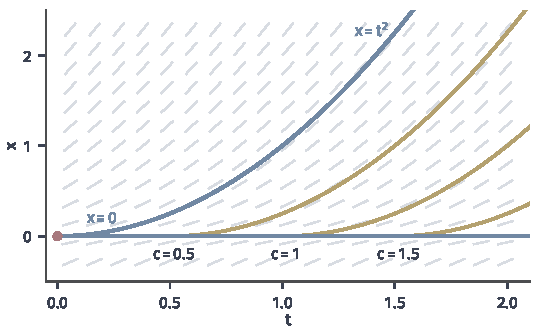
\includegraphics[width=92mm]{figures/06-differential-equations/01-ordinary-differential-equations/matplotlib/odeex-sqrt-funnel/figure.pdf}
  \caption{初值问题~\eqref{eq:odeex-sqrt}的多个解。短线是方向场，红点是初值$(0,0)$。蓝线是$x\equiv0$与$x=t^2$，黄线是在$t=c$时离开零线的解$x_c$，$c=0.5,1,1.5$。任意$c\geq0$都给出一条解。}
  \label{fig:odeex-sqrt-funnel}
\end{BookInlineFigure}

为什么连续性不足以挑出一条解？$x$接近$0$时，箭头斜率$2\sqrt{\lvert x\rvert}$相对于$\lvert x\rvert$大得不成比例：比值$2/\sqrt{\lvert x\rvert}$趋于无穷。于是离开零线一点点就有足够的速度继续远离，离开零线并不需要一个有限的“推力”。

多解还解释了为什么证明中要抽子列。考虑方程
\[
 \dot x=2\operatorname{sgn}(x)\sqrt{\lvert x\rvert},\qquad x(0)=0,
\]
它同样有解$x\equiv0$和$x=\pm t^2$。若折线的初值恰好是$0$，它恒为零；但若初值带一个微小的扰动$x^{(0)}=(-1)^N/N^2$，比如计算时的舍入，$N$为偶数和奇数时折线会走向不同的解。

取$N$为偶数，步长$h=\delta/N$，其中$\delta=1$。令$s_k=\sqrt{x^{(k)}}$，由式~\eqref{eq:odeex-euler-node}，
\[
 s_{k+1}^2=s_k^2+2hs_k.
\]
当$s_k\geq h/4$时，$(s_k+h/2)^2=s_k^2+hs_k+h^2/4\leq s_k^2+2hs_k$，所以$s_{k+1}\geq s_k+h/2$。而$s_0=1/N=h$，于是对所有$k$，
\[
 x^{(k)}\geq\bigl(s_0+kh/2\bigr)^2\geq\Bigl(\frac{t_k}{2}\Bigr)^2.
\]

奇数$N$的折线是偶数情形的镜像。所以偶数列的极限至少是$t^2/4$，奇数列的极限至多是$-t^2/4$，整列折线没有极限，如图~\ref{fig:odeex-odd-sqrt-euler}所示。紧性只给出“有收敛的子列”，不同子列可以收敛到不同的解。

\begin{BookInlineFigure}
  \centering
  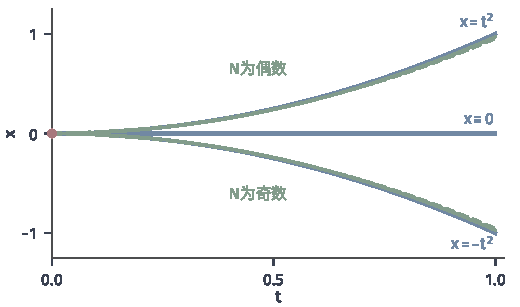
\includegraphics[width=88mm]{figures/06-differential-equations/01-ordinary-differential-equations/matplotlib/odeex-odd-sqrt-euler/figure.pdf}
  \caption{$\dot x=2\operatorname{sgn}(x)\sqrt{\lvert x\rvert}$的Euler折线，初值$x^{(0)}=(-1)^N/N^2$，步长$1/N$。绿色虚线$N=20,21$，绿色实线$N=80,81$，蓝线是从$(0,0)$出发的三条解。偶数$N$贴近$t^2$，奇数$N$贴近$-t^2$，整列不收敛。}
  \label{fig:odeex-odd-sqrt-euler}
\end{BookInlineFigure}

\paragraph{紧性只属于有限维}
证明的第二步用了“一致有界且等度连续的曲线族相对紧”。它的前提是每个时刻的取值落在一个紧集中，而$\mathbb{R}^{n}$的闭球恰好是紧的。在无限维空间中闭球不紧，这一步不能照搬，结论也确实会失败。

设$c_0$是收敛到零的实数列$\bm{x}=(x_1,x_2,\ldots)$组成的空间，范数取各坐标绝对值的上确界，记为$\lVert\bm{x}\rVert_{\infty}$，它是完备的。定义$\bm{f}:c_0\to c_0$，
\[
 \bigl(\bm{f}(\bm{x})\bigr)_n=2\sqrt{\lvert x_n\rvert}+\frac{1}{n+1},\qquad n\geq1.
\]
第一项随$n\to\infty$趋于零，第二项也是，所以$\bm{f}(\bm{x})\in c_0$。对实数$a,b$，有
\[
 \lvert\sqrt{\lvert a\rvert}-\sqrt{\lvert b\rvert}\rvert\leq\sqrt{\lvert a-b\rvert}.
\]
逐坐标使用它，得到
\[
 \lVert\bm{f}(\bm{x})-\bm{f}(\bm{y})\rVert_{\infty}\leq2\sqrt{\lVert\bm{x}-\bm{y}\rVert_{\infty}},
\]
所以$\bm{f}$连续。

假设$\bm{x}(t)$是$[0,\delta)$上取值于$c_0$的解，$\bm{x}(0)=\bm{0}$。在范数下可微蕴含每个坐标可微，所以每个坐标满足$\dot x_n=2\sqrt{\lvert x_n\rvert}+1/(n+1)>0$。于是$x_n(t)>0$对$t>0$成立，并且
\[
 \frac{\mathrm{d}}{\mathrm{d}t}\sqrt{x_n}=\frac{\dot x_n}{2\sqrt{x_n}}\geq1.
\]
从$s>0$积分到$t$，再令$s\downarrow0$，得到$\sqrt{x_n(t)}\geq t$，即对所有$n$，
\[
 x_n(t)\geq t^2.
\]
每个坐标都不低于同一个正数，这与$\bm{x}(t)\in c_0$矛盾。因此这个连续方程在$c_0$中没有解。

图~\ref{fig:odeex-c0-coordinates}算出了各坐标的实际取值。右端的序列在$t=0$时衰减，解的坐标却被$t^2$托住，在任何$t>0$时都不再衰减到零。$\bm{f}$的连续性和局部有界性都在，只是缺了紧性。

\begin{BookInlineFigure}
  \centering
  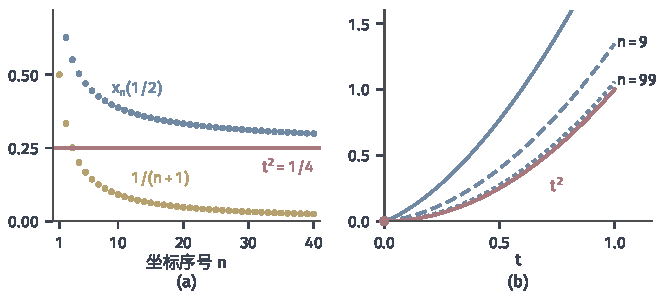
\includegraphics[width=112mm]{figures/06-differential-equations/01-ordinary-differential-equations/matplotlib/odeex-c0-coordinates/figure.pdf}
  \caption{$c_0$中无解方程的坐标。各坐标单独满足$\dot x_n=2\sqrt{x_n}+1/(n+1)$，$x_n(0)=0$，由数值积分算出。(a)$t=1/2$时的取值，蓝点$x_n(1/2)$都在红线$t^2=1/4$之上，黄点$1/(n+1)$是右端在$t=0$的序列。(b)蓝线为$n=1,9,99$时的$x_n(t)$，都在红线$t^2$之上，$n$增大时趋于$t^2$而不趋于$0$。}
  \label{fig:odeex-c0-coordinates}
\end{BookInlineFigure}

\section{唯一性}
\label{sec:odeex-uniqueness}

漏斗状的多解出现在$\dot x=2\sqrt{\lvert x\rvert}$的零线上，那里右端随状态变化得太快。反过来想，什么样的右端能阻止两条解分开？设$\bm{u},\bm{v}$是同一初值的两条解，它们的差的变化率是$\bm{f}(t,\bm{u})-\bm{f}(t,\bm{v})$。若这个量能用差本身来控制，两条解一开始重合，就没有东西推动它们分开。

\paragraph{状态方向的Lipschitz条件}
把“右端的变化能用状态差控制”写成条件。下面只比较同一时刻的两个状态，时间方向没有光滑性要求。

\begin{definition}[状态方向的局部Lipschitz条件]
\label{def:odeex-local-lipschitz}
设$\bm{D}\subseteq\mathbb{R}\times\mathbb{R}^{n}$开，$\bm{f}:\bm{D}\to\mathbb{R}^{n}$。若对每点$(t_\ast,\bm{x}_\ast)\in\bm{D}$，存在它的邻域$\bm{U}\subseteq\bm{D}$和常数$L\geq0$，使对$\bm{U}$中所有同一时刻的两点$(t,\bm{x}),(t,\bm{y})$都有
\begin{equation}
 \lVert\bm{f}(t,\bm{x})-\bm{f}(t,\bm{y})\rVert_2\leq L\lVert\bm{x}-\bm{y}\rVert_2,
 \label{eq:odeex-lipschitz}
\end{equation}
就称$\bm{f}$在状态方向\term{局部Lipschitz连续}（locally Lipschitz continuous），且该性质对时间局部一致。
\end{definition}

定义里的“局部一致”指同一个$L$对邻域内所有时刻都有效。几何上，固定时刻后，以$(\bm{x},\bm{f}(t,\bm{x}))$为顶点、斜率$L$的双锥把邻域内其余部分的图像都关在里面。图~\ref{fig:odeex-lipschitz-secants}比较三个函数。

\begin{BookInlineFigure}
  \centering
  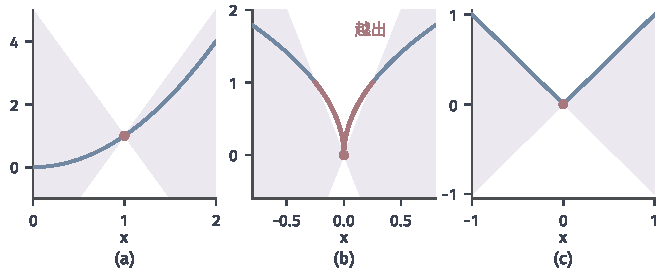
\includegraphics[width=112mm]{figures/06-differential-equations/01-ordinary-differential-equations/matplotlib/odeex-lipschitz-secants/figure.pdf}
  \caption{状态方向的Lipschitz条件。蓝线是函数图像，红点是基点，紫色区域是斜率$L$的双锥。(a)$x^2$在$[0,2]$上，基点$x=1$，$L=4$，图像在双锥内。(b)$2\sqrt{\lvert x\rvert}$，基点$x=0$，$L=4$，红色部分越出双锥；增大$L$只能缩小越出的范围，不能消除。(c)$\lvert x\rvert$，$L=1$，在基点不可微，图像仍在双锥内。}
  \label{fig:odeex-lipschitz-secants}
\end{BookInlineFigure}

图(a)的$x^2$在$[0,2]$上满足条件：
\[
 \lvert x^2-y^2\rvert=\lvert x+y\rvert\,\lvert x-y\rvert\leq4\lvert x-y\rvert.
\]
它在整条实轴上没有统一的$L$，这正是“局部”二字的用处。图(b)的$2\sqrt{\lvert x\rvert}$在原点不满足条件，这与多解的出现位置一致。图(c)说明Lipschitz条件比可微弱，折角并不妨碍它。

验证条件最常用的办法是求导。若$\partial_{\bm{x}}\bm{f}$存在且在$\bm{D}$上连续，在一个球形邻域内连接$\bm{x},\bm{y}$的线段上积分，得到
\[
 \bm{f}(t,\bm{x})-\bm{f}(t,\bm{y})
 =\int_0^1\partial_{\bm{x}}\bm{f}\bigl(t,\bm{y}+\theta(\bm{x}-\bm{y})\bigr)(\bm{x}-\bm{y})\,\mathrm{d}\theta.
\]
在紧邻域上取$L$为$\lVert\partial_{\bm{x}}\bm{f}\rVert_2$的最大值，就得到式~\eqref{eq:odeex-lipschitz}。

\paragraph{主要思想：积分方程是不动点问题}
积分方程~\eqref{eq:odeex-integral}把解刻画成一个自洽条件。给定一条曲线$\bm{u}$，沿它读出箭头，积分出一条新曲线，记为
\begin{equation}
 (\mathcal{T}\bm{u})(t)=\bm{x}_0+\int_{t_0}^{t}\bm{f}(s,\bm{u}(s))\,\mathrm{d}s.
 \label{eq:odeex-picard-map}
\end{equation}
解就是$\mathcal{T}$的不动点：把它代入，得到的还是它自己。把曲线看成无限维向量（每个时刻是一个坐标），$\mathcal{T}$是这个向量空间上的一个映射，初值问题就成了解方程$\bm{x}=\mathcal{T}\bm{x}$。

解这个方程最朴素的办法是反复代入。从常值曲线$\bm{x}^{(0)}(t)\equiv\bm{x}_0$出发，令
\begin{equation}
 \bm{x}^{(k+1)}=\mathcal{T}\bm{x}^{(k)},\quad k=0,1,\ldots,
 \label{eq:odeex-picard-iteration}
\end{equation}
这一列曲线称为\term{Picard迭代}（Picard iteration）。本节中上标$(k)$表示迭代次数，每个$\bm{x}^{(k)}$是一整条曲线。

\begin{example}[指数函数的Picard迭代]
\label{ex:odeex-picard-exp}
取$\dot x=x$，$x(0)=1$，此时$(\mathcal{T}u)(t)=1+\int_0^tu(s)\,\mathrm{d}s$。前几步分别是
\[
 x^{(0)}=1,\quad x^{(1)}=1+t,\quad x^{(2)}=1+t+\frac{t^2}{2}.
\]

设$x^{(k)}(t)=\sum_{j=0}^{k}t^j/j!$，代入式~\eqref{eq:odeex-picard-map}，逐项积分得到
\[
 x^{(k+1)}(t)=1+\sum_{j=0}^{k}\frac{t^{j+1}}{(j+1)!}=\sum_{j=0}^{k+1}\frac{t^j}{j!}.
\]
所以Picard迭代就是指数级数的部分和。在$[0,1]$上，余项满足
\[
 \lvert\mathrm{e}^t-x^{(k)}(t)\rvert\leq\frac{\mathrm{e}}{(k+1)!}.
\]
\end{example}

图~\ref{fig:odeex-picard-exp}显示，每迭代一次，曲线多贴合真解一段。对这个例子，迭代既不是在时间方向上推进，也不是逐点修正，而是每次把整条曲线替换一遍。

\begin{BookInlineFigure}
  \centering
  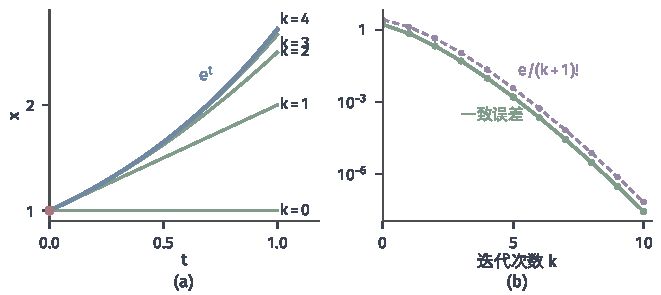
\includegraphics[width=112mm]{figures/06-differential-equations/01-ordinary-differential-equations/matplotlib/odeex-picard-exp/figure.pdf}
  \caption{$\dot x=x$，$x(0)=1$的Picard迭代。(a)绿线是$x^{(0)},\ldots,x^{(4)}$，蓝线是真解$\mathrm{e}^t$，红点是初值。(b)$[0,1]$上的一致误差（绿线）与上界$\mathrm{e}/(k+1)!$（紫色虚线），纵轴为对数坐标；衰减比任何几何级数都快。}
  \label{fig:odeex-picard-exp}
\end{BookInlineFigure}

\paragraph{为什么要缩短时间窗}
要保证迭代一般都收敛，自然想到压缩映射定理：完备度量空间上的压缩映射有唯一不动点，迭代从任何初值出发都收敛到它，可参考\BookChapterRef{chap:metric-space-maps}{卷四第3章“度量空间上的映射”}，那里也证明了区间上的连续函数在一致距离下完备。下面估计$\mathcal{T}$对曲线距离的作用。

设$\bm{u},\bm{v}$是两条曲线，$(s,\bm{u}(s))$和$(s,\bm{v}(s))$都在Lipschitz条件成立的盒子内。对$\lvert t-t_0\rvert\leq\delta$，由积分的范数不等式与式~\eqref{eq:odeex-lipschitz}，
\[
 \lVert(\mathcal{T}\bm{u})(t)-(\mathcal{T}\bm{v})(t)\rVert_2
 \leq\Bigl\lvert\int_{t_0}^{t}L\lVert\bm{u}(s)-\bm{v}(s)\rVert_2\,\mathrm{d}s\Bigr\rvert
 \leq L\delta\sup_{s}\lVert\bm{u}(s)-\bm{v}(s)\rVert_2.
\]

$\mathcal{T}$对距离的放大倍数至多是$L\delta$。积分把两条曲线的差沿时间累积，累积的时间越短，差就越小；$\delta$足够小时，这个映射就是压缩的。

图~\ref{fig:odeex-integral-smoothing}对$\dot x=x^2$，$x(0)=1$演示了这一点。两条任意选取的曲线在$[-1/8,1/8]$上一致距离约为$1.31$，经$\mathcal{T}$作用后，距离约为$0.125$，比值约$0.095$，小于这里的压缩常数$1/2$。

\begin{BookInlineFigure}
  \centering
  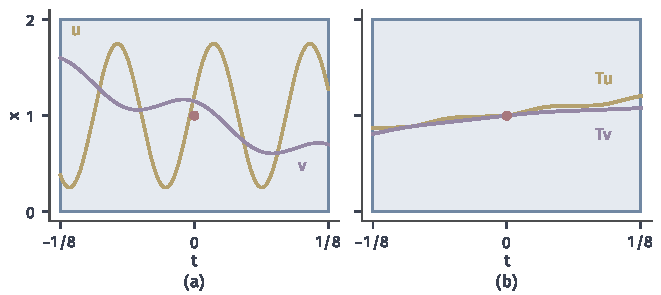
\includegraphics[width=112mm]{figures/06-differential-equations/01-ordinary-differential-equations/matplotlib/odeex-integral-smoothing/figure.pdf}
  \caption{积分映射缩小曲线距离。方程为$\dot x=x^2$，$x(0)=1$，浅蓝矩形是$\lvert t\rvert\leq1/8$、$\lvert x-1\rvert\leq1$的盒子。(a)盒内两条任取的曲线$u$（黄）和$v$（紫）。(b)它们的像$\mathcal{T}u$和$\mathcal{T}v$，都过红色初值点，振荡被积分抹平，一致距离由约$1.31$降为约$0.125$。}
  \label{fig:odeex-integral-smoothing}
\end{BookInlineFigure}

只缩短时间窗还不够，$\mathcal{T}$要把所选的曲线集合映回自身，否则迭代中途可能离开盒子，式~\eqref{eq:odeex-lipschitz}就不能再用。第~\ref{sec:odeex-local-existence}节的锥形估计恰好处理这件事。把这两个要求放在一起，就是\term{Picard--Lindelöf定理}（Picard--Lindelöf theorem）。

\begin{theorem}[Picard--Lindelöf定理]
\label{thm:odeex-picard-lindelof}
设$\bm{f}:\bm{D}\to\mathbb{R}^{n}$，$\bm{Q}=[t_0-a,t_0+a]\times\bm{B}_b\subseteq\bm{D}$，$\bm{f}$在$\bm{Q}$上连续，并存在$M,L>0$，使$\lVert\bm{f}\rVert_2\leq M$与式~\eqref{eq:odeex-lipschitz}在$\bm{Q}$上成立。令
\begin{equation}
 \delta=\min\Bigl\{a,\frac{b}{M},\frac{1}{2L}\Bigr\},\qquad I_\delta=[t_0-\delta,t_0+\delta].
 \label{eq:odeex-picard-window}
\end{equation}
则：
\begin{enumerate}
 \item 初值问题~\eqref{eq:odeex-ivp}在$I_\delta$上有经典解$\bm{x}$，其取值都在$\bm{B}_b$中；
 \item 若$I'\subseteq I_\delta$是含$t_0$的区间，$\bm{y}$是$I'$上的任一经典解，则$\bm{y}=\bm{x}$在$I'$上成立；
 \item Picard迭代~\eqref{eq:odeex-picard-iteration}在$I_\delta$上一致收敛到$\bm{x}$，且对$k\geq1$，
 \begin{equation}
 \lVert\bm{x}^{(k)}-\bm{x}\rVert_{\infty}\leq2^{1-k}\lVert\bm{x}^{(1)}-\bm{x}^{(0)}\rVert_{\infty},\qquad
 \lVert\bm{x}^{(k)}-\bm{x}\rVert_{\infty}\leq\lVert\bm{x}^{(k)}-\bm{x}^{(k-1)}\rVert_{\infty}.
 \label{eq:odeex-picard-error}
 \end{equation}
\end{enumerate}
\end{theorem}

\begin{proof}
\emph{选取空间。}记$\lVert\bm{y}\rVert_{\infty}$为$\lVert\bm{y}(t)\rVert_2$在$I_\delta$上的最大值，$C(I_\delta;\mathbb{R}^{n})$在这个范数下完备。令
\[
 \mathcal{X}=\bigl\{\bm{u}\in C(I_\delta;\mathbb{R}^{n}):\lVert\bm{u}(t)-\bm{x}_0\rVert_2\leq b,\ \forall t\in I_\delta\bigr\}.
\]
$\mathcal{X}$是闭集，一致收敛保持逐点的不等式，所以$\mathcal{X}$在一致距离下是完备度量空间；它含常值曲线$\bm{x}_0$，非空。

\emph{映回自身。}设$\bm{u}\in\mathcal{X}$。由$\delta\leq a$，点$(s,\bm{u}(s))$对$s\in I_\delta$都在$\bm{Q}$中，$s\mapsto\bm{f}(s,\bm{u}(s))$连续，积分有定义，$\mathcal{T}\bm{u}$连续。由$\delta\leq b/M$，
\[
 \lVert(\mathcal{T}\bm{u})(t)-\bm{x}_0\rVert_2
 \leq\Bigl\lvert\int_{t_0}^{t}\lVert\bm{f}(s,\bm{u}(s))\rVert_2\,\mathrm{d}s\Bigr\rvert
 \leq M\lvert t-t_0\rvert\leq b.
\]
所以$\mathcal{T}\bm{u}\in\mathcal{X}$。

\emph{压缩。}对$\bm{u},\bm{v}\in\mathcal{X}$，点$(s,\bm{u}(s)),(s,\bm{v}(s))$都在$\bm{Q}$中，前面的估计给出
\[
 \lVert\mathcal{T}\bm{u}-\mathcal{T}\bm{v}\rVert_{\infty}\leq L\delta\lVert\bm{u}-\bm{v}\rVert_{\infty}\leq\frac12\lVert\bm{u}-\bm{v}\rVert_{\infty}.
\]

\emph{不动点。}由压缩映射定理，$\mathcal{T}$在$\mathcal{X}$中有唯一不动点$\bm{x}$，Picard迭代从$\bm{x}^{(0)}\equiv\bm{x}_0\in\mathcal{X}$出发一致收敛到$\bm{x}$，其先验误差界和后验误差界取压缩常数$q=1/2$，就是式~\eqref{eq:odeex-picard-error}。不动点满足积分方程~\eqref{eq:odeex-integral}，因而是经典解。结论1和结论3得证。

\emph{任何解都留在盒内。}设$\bm{y}$是$I'$上的解。只看$t\geq t_0$的一侧，另一侧相同。令$t^\ast$为使$\bm{y}$在$[t_0,t]\cap I'$上取值于$\bm{B}_b$的$t$的上确界。在$[t_0,t^\ast)\cap I'$上点$(s,\bm{y}(s))$在$\bm{Q}$中，所以$\lVert\bm{y}(t)-\bm{x}_0\rVert_2\leq M(t-t_0)$在其上成立。

若$t^\ast$小于$I'$的右端点，则$t^\ast<t_0+\delta$，由连续性，
\[
 \lVert\bm{y}(t^\ast)-\bm{x}_0\rVert_2\leq M(t^\ast-t_0)<M\delta\leq b.
\]
这是严格不等式，$\bm{y}$在$t^\ast$之后一小段时间内还在球内，与上确界的定义矛盾。所以$\bm{y}$在$I'$上始终留在$\bm{B}_b$中。

\emph{唯一性。}两条解$\bm{x},\bm{y}$在$I'$上都留在盒内，都满足积分方程。记$e=\sup_{t\in I'}\lVert\bm{x}(t)-\bm{y}(t)\rVert_2$，它不超过$2b$，是有限数。相减并用式~\eqref{eq:odeex-lipschitz}，
\[
 \lVert\bm{x}(t)-\bm{y}(t)\rVert_2\leq L\delta\,e\leq\frac12e.
\]
对$t\in I'$取上确界，得$e\leq e/2$，即$e=0$，结论2得证。
\end{proof}

定理中各条件分工明确。$\bm{Q}\subseteq\bm{D}$让方程有定义；$\delta\leq b/M$让$\mathcal{T}$不把曲线带出盒子；$\delta\leq1/(2L)$让距离缩小；连续性让积分有定义，并使不动点是经典解。完备性保证迭代的柯西列有极限，这里用不到任何紧性。

\paragraph{计算过程}
Picard迭代的每一步都要计算一条曲线的积分，下面用$\dot x=x^2$，$x(0)=1$手算到第三轮，完整走一遍。取$a=1/2$，$b=1$，由图~\ref{fig:odeex-lipschitz-secants}(a)的计算，$M=4$，$L=4$，所以
\[
 \delta=\min\Bigl\{\frac12,\frac14,\frac18\Bigr\}=\frac18,\qquad q=L\delta=\frac12.
\]

\needspace{6\baselineskip}
\paragraph{变量}
\begin{itemize}
 \item $x^{(k)}$：第$k$轮的曲线，定义在$I_\delta=[-1/8,1/8]$上，例中都是多项式；
 \item $\Delta^{(k)}$：相邻两轮的一致距离$\lVert x^{(k)}-x^{(k-1)}\rVert_{\infty}$，用于后验误差界；
 \item $\varepsilon$：给定的误差容许值，例中取$2\times10^{-3}$。
\end{itemize}

\needspace{6\baselineskip}
\paragraph{初始化}
令$\bm{x}^{(0)}(t)\equiv\bm{x}_0$。例中$x^{(0)}=1$。

\needspace{6\baselineskip}
\paragraph{每轮更新}
对$k=0,1,\ldots$，依次执行：
\begin{enumerate}
 \item 由式~\eqref{eq:odeex-picard-iteration}，把$\bm{x}^{(k)}$代入右端并积分，得到$\bm{x}^{(k+1)}$。

 例中第一轮的被积函数是$1$，所以
 \[
 x^{(1)}(t)=1+t.
 \]
 第二轮对$(1+s)^2$积分，得到
 \[
 x^{(2)}(t)=1+t+t^2+\frac{t^3}{3}.
 \]
 第三轮对$(1+s+s^2+s^3/3)^2$积分，得到
 \[
 x^{(3)}(t)=1+t+t^2+t^3+\frac23t^4+\frac13t^5+\frac19t^6+\frac{1}{63}t^7.
 \]
 \item 计算$\Delta^{(k+1)}$。例中相邻两轮的差都在$t=1/8$处取到最大模，于是
 \[
 \Delta^{(1)}=\frac18,\quad \Delta^{(2)}\approx1.63\times10^{-2},\quad \Delta^{(3)}\approx1.48\times10^{-3}.
 \]
 \item 若后验误差界$q\Delta^{(k+1)}/(1-q)$不超过$\varepsilon$，就停止，否则继续。由式~\eqref{eq:odeex-picard-error}，$q=1/2$时这个界就是$\Delta^{(k+1)}$。

 例中$\Delta^{(2)}>\varepsilon$，第二轮后继续；$\Delta^{(3)}\leq\varepsilon$，第三轮后停止。
\end{enumerate}

最终得到$x^{(3)}$，它在$[-1/8,1/8]$上与真解的误差被保证不超过$1.48\times10^{-3}$。实际误差约为$1.06\times10^{-4}$，比界小一个数量级。

图~\ref{fig:odeex-picard-square}(a)显示迭代在时间窗内很快贴合真解，窗外贴合得较慢，越靠近真解的奇点$t=1$差得越远。图(b)比较实际误差和先验界$2^{1-k}\cdot1/8$，先验界用的是全局的$q=1/2$，实际误差衰减得快得多。

\begin{BookInlineFigure}
  \centering
  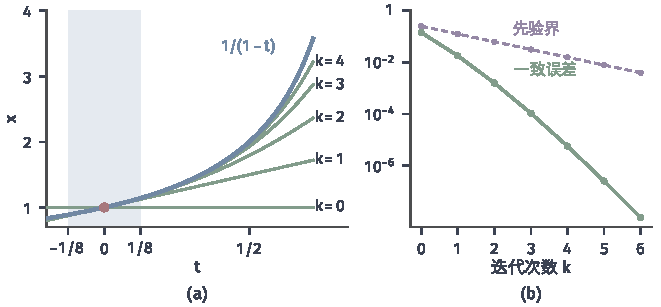
\includegraphics[width=112mm]{figures/06-differential-equations/01-ordinary-differential-equations/matplotlib/odeex-picard-square/figure.pdf}
  \caption{$\dot x=x^2$，$x(0)=1$的Picard迭代。(a)绿线是$x^{(0)},\ldots,x^{(4)}$，蓝线是真解，浅蓝带是时间窗$[-1/8,1/8]$。(b)时间窗上的一致误差（绿线）与先验界$2^{1-k}\cdot\tfrac18$（紫色虚线），纵轴为对数坐标。}
  \label{fig:odeex-picard-square}
\end{BookInlineFigure}

\paragraph{时间窗不必缩到$1/(2L)$}
定理中的$1/(2L)$是为了让$\mathcal{T}$在一步之内就成为压缩映射。例~\ref{ex:odeex-picard-exp}在$[0,1]$上有$L\delta=1$，不是压缩，迭代却收敛得比几何级数还快。原因是误差要累积多次才会放大，而累积的时间区域越来越窄。

设$\delta'=\min\{a,b/M\}$，定义域换成$I_{\delta'}$。前面“映回自身”的论证只用了$\delta'\leq a$与$\delta'\leq b/M$，所以$\mathcal{T}$仍把相应的$\mathcal{X}$映回自身，迭代都有定义。下面对$k\geq0$归纳证明，对$t\in I_{\delta'}$，
\begin{equation}
 \lVert\bm{x}^{(k+1)}(t)-\bm{x}^{(k)}(t)\rVert_2\leq\frac{ML^{k}\lvert t-t_0\rvert^{k+1}}{(k+1)!}.
 \label{eq:odeex-picard-factorial}
\end{equation}

$k=0$时，左端是$\bm{f}(s,\bm{x}_0)$积分的范数，被积函数的范数不超过$M$，所以不超过$M\lvert t-t_0\rvert$。设$k-1$时成立，对$t\geq t_0$，由式~\eqref{eq:odeex-lipschitz}，
\[
 \lVert\bm{x}^{(k+1)}(t)-\bm{x}^{(k)}(t)\rVert_2
 \leq L\int_{t_0}^{t}\frac{ML^{k-1}(s-t_0)^{k}}{k!}\,\mathrm{d}s
 =\frac{ML^{k}(t-t_0)^{k+1}}{(k+1)!}.
\]
$t<t_0$的情形相同。

式~\eqref{eq:odeex-picard-factorial}的右端对$k$求和收敛，和不超过$M(\mathrm{e}^{L\delta'}-1)/L$，所以$\bm{x}^{(k)}$一致收敛，其极限是$\mathcal{T}$的不动点。两个不动点的差用同样的归纳，得到对任意$k$，
\[
 \lVert\bm{u}(t)-\bm{v}(t)\rVert_2\leq2b\,\frac{(L\lvert t-t_0\rvert)^{k}}{k!},
\]
令$k\to\infty$，差为零。任何解都留在盒内的论证也只用到$\delta'\leq b/M$。因此解在整个$I_{\delta'}$上存在且唯一，时间窗的长度由$a$和$b/M$决定，不受$L$限制；$L$只影响收敛的快慢。

\paragraph{Lipschitz条件只是充分条件}
定理给出的是唯一性的充分条件，并不必要。考虑方向相反的方程
\[
 \dot x=-2\operatorname{sgn}(x)\sqrt{\lvert x\rvert}.
\]
它在原点同样不满足Lipschitz条件。但右端关于$x$单调不增，两条解$u,v$之差满足
\[
 \frac{\mathrm{d}}{\mathrm{d}t}(u-v)^2=2(u-v)\bigl(f(u)-f(v)\bigr)\leq0.
\]
所以差只会减小，初值相同的两条解在$t$增大的方向上不会分开，向前唯一。

图~\ref{fig:odeex-one-sided-merge}显示了这个方程的解：从$x_0$出发的解是$\operatorname{sgn}(x_0)(\sqrt{\lvert x_0\rvert}-t)^2$，在$t=\sqrt{\lvert x_0\rvert}$到达零线后停在那里，不同的解在有限时间内合并。把时间倒过来，方程变成式~\eqref{eq:odeex-sqrt}的奇函数版本，从零线出发可以有多条解，所以向后不唯一。这里的唯一性来自单调性，与Lipschitz条件无关。

\begin{BookInlineFigure}
  \centering
  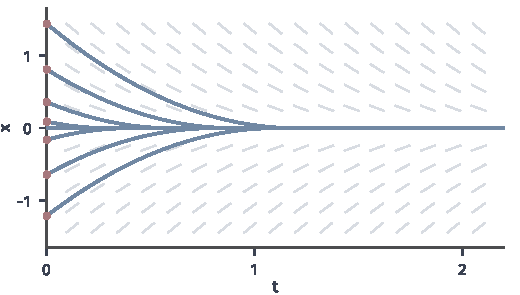
\includegraphics[width=88mm]{figures/06-differential-equations/01-ordinary-differential-equations/matplotlib/odeex-one-sided-merge/figure.pdf}
  \caption{$\dot x=-2\operatorname{sgn}(x)\sqrt{\lvert x\rvert}$的解。短线是方向场，红点是不同的初值，蓝线是相应的解，在有限时间内汇入零线。向前的解由初值确定，向后从零线出发则有多个可能。}
  \label{fig:odeex-one-sided-merge}
\end{BookInlineFigure}

\paragraph{Lipschitz常数要对时间局部一致}
定义~\ref{def:odeex-local-lipschitz}要求$L$在邻域内对时间一致。如果每个时刻各有一个常数，但常数随时间无界，唯一性也会失败。令$\operatorname{clip}(x;0,t^2)$表示把$x$截断到$[0,t^2]$，定义
\begin{equation}
 f(t,x)=\begin{cases}\dfrac{2}{t}\operatorname{clip}(x;0,t^2),&t>0,\\0,&t\leq0.\end{cases}
 \label{eq:odeex-clip}
\end{equation}

由$0\leq\operatorname{clip}\leq t^2$，有$\lvert f(t,x)\rvert\leq2t$，所以$f$在$t=0$处连续，从而在$\mathbb{R}^{2}$上连续。固定$t>0$，$f$关于$x$是Lipschitz的，常数为$2/t$；固定$t\leq0$，$f$恒为零。每个时刻单独看都满足条件，但常数$2/t$在$t\to0$时无界。

对每个$c\in[0,1]$，曲线$x=ct^2$满足$0\leq x\leq t^2$，右端等于$2ct$，恰是它的导数。所以从$x(0)=0$出发有无穷多条解，如图~\ref{fig:odeex-time-lipschitz}所示。两条解的差以$2/t$的相对速率增长，这个速率在$t=0$附近的积分发散，足以从零差产生非零差。

\begin{BookInlineFigure}
  \centering
  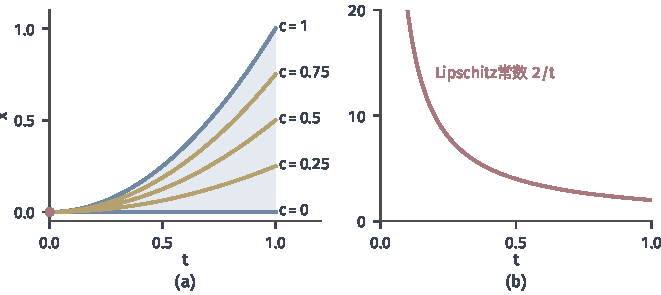
\includegraphics[width=112mm]{figures/06-differential-equations/01-ordinary-differential-equations/matplotlib/odeex-time-lipschitz/figure.pdf}
  \caption{Lipschitz常数对时间不一致导致多解。(a)方程~\eqref{eq:odeex-clip}的解$x=ct^2$，浅蓝区域$0\leq x\leq t^2$内，$c$取$0,0.25,0.5,0.75,1$，都从红点出发。(b)固定时刻的Lipschitz常数$2/t$，在$t\to0$时无界。}
  \label{fig:odeex-time-lipschitz}
\end{BookInlineFigure}

\paragraph{紧性与完备性}
Peano和Picard两条路线用的工具不同，结论的强弱也不同，表~\ref{tab:odeex-peano-picard}把它们放在一起。

\begin{BookInlineTable}
  \centering
  \caption{两条存在性路线的对比}
  \label{tab:odeex-peano-picard}
  \begin{tabular}{lll}
    \toprule
     & Peano路线 & Picard路线 \\
    \midrule
    右端条件 & 连续 & 连续，状态方向Lipschitz \\
    逼近对象 & Euler折线 & Picard迭代 \\
    收敛来源 & 紧性，只有子列 & 完备性，整列收敛 \\
    结论 & 至少一个解 & 恰有一个解，有误差界 \\
    无限维空间 & 可能无解 & 证明不变，结论成立 \\
    \bottomrule
  \end{tabular}
\end{BookInlineTable}

最后一行值得注意。Picard路线只用到空间的完备性和范数不等式，状态空间换成任何完备的赋范空间，证明的步骤不变，只需假设盒子上$\bm{f}$有界且满足Lipschitz条件。第~\ref{sec:odeex-local-existence}节$c_0$上的反例恰好不满足Lipschitz条件。

\section{最大延拓}
\label{sec:odeex-maximal}

Picard--Lindelöf定理只保证一小段时间。到达时间窗的尽头后，把终点当作新的初值再解一段，解就能接着往前走。这个过程能继续多久，走不下去时发生了什么？本节在定义~\ref{def:odeex-local-lipschitz}的条件下回答。以下总设$\bm{D}\subseteq\mathbb{R}\times\mathbb{R}^{n}$开，$\bm{f}:\bm{D}\to\mathbb{R}^{n}$连续，并在状态方向局部Lipschitz连续，该性质对时间局部一致。

\paragraph{相容的局部解}
拼接之前要确认，两段局部解在重叠处不会打架。局部唯一性只在一个小窗内成立，下面的引理把它传播到任意长的公共区间上，办法是看两条解重合的时刻组成的集合。

\begin{lemma}[公共区间上的唯一性]
\label{lem:odeex-common-uniqueness}
设$\bm{x}_1,\bm{x}_2$分别是区间$I_1,I_2$上的经典解，$I_1\cap I_2$含$t_0$，且$\bm{x}_1(t_0)=\bm{x}_2(t_0)$。则$\bm{x}_1=\bm{x}_2$在$I_1\cap I_2$上成立。
\end{lemma}

\begin{proof}
记$I=I_1\cap I_2$，它是区间。令$S=\{t\in I:\bm{x}_1(t)=\bm{x}_2(t)\}$，它含$t_0$。两条解连续，所以$S$在$I$中闭。

下面证明$S$在$I$中开。任取$t^\ast\in S$，记$\bm{x}^\ast=\bm{x}_1(t^\ast)$。在$(t^\ast,\bm{x}^\ast)$的邻域内，由定义~\ref{def:odeex-local-lipschitz}，可以取一个盒子和常数$M,L$，使定理~\ref{thm:odeex-picard-lindelof}的条件成立，得到时间窗$[t^\ast-\delta,t^\ast+\delta]$。

$\bm{x}_1,\bm{x}_2$在区间$I\cap[t^\ast-\delta,t^\ast+\delta]$上都是以$(t^\ast,\bm{x}^\ast)$为初值的经典解，由定理的结论2，它们都等于窗上的唯一解，所以这段区间包含在$S$中。

$I$是连通的，$S$是它的非空开闭子集，于是$S=I$。
\end{proof}

图~\ref{fig:odeex-gluing}(a)画的是两段解的重叠，引理保证重叠部分是同一条曲线。图(b)是证明的核心：若两条解有“第一次分开”的时刻$t^\ast$，在该时刻的状态附近局部唯一性就被破坏了，所以这样的时刻不存在。

\begin{BookInlineFigure}
  \centering
  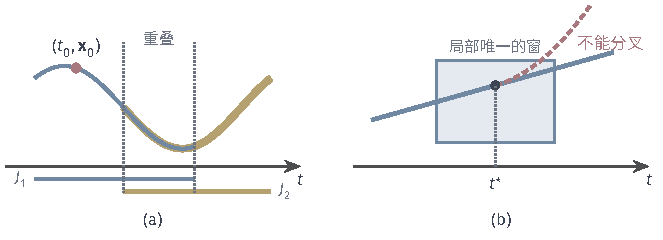
\includegraphics[width=112mm]{figures/06-differential-equations/01-ordinary-differential-equations/tikz/odeex-gluing/figure.pdf}
  \caption{局部解的相容性。(a)区间$J_1$（蓝）与$J_2$（黄）上的两段解经过同一初值，在重叠的时间段内是同一条曲线，并起来是更长区间上的解。(b)若两条解在$t^\ast$之后分开（红色虚线），在$(t^\ast,\bm{x}(t^\ast))$的小窗（浅蓝矩形）内就有两个解，与局部唯一性矛盾。}
  \label{fig:odeex-gluing}
\end{BookInlineFigure}

\paragraph{最大解}
有了相容性，就可以把所有局部解并起来。设$\bm{x}$是区间$I$上的解，$\tilde{\bm{x}}$是区间$\tilde I\supsetneq I$上的解，且$\tilde{\bm{x}}$在$I$上等于$\bm{x}$，就称$\tilde{\bm{x}}$是$\bm{x}$的一个\term{解的延拓}（continuation of a solution）。不能再延拓的解称为\term{最大解}（maximal solution），它的定义区间称为\term{最大存在区间}（maximal interval of existence）。

\begin{theorem}[最大解]
\label{thm:odeex-maximal}
对每点$(t_0,\bm{x}_0)\in\bm{D}$，初值问题~\eqref{eq:odeex-ivp}存在唯一的最大解$\bm{x}:I_{\max}\to\mathbb{R}^{n}$，其中$I_{\max}=(\omega_-,\omega_+)$是含$t_0$的开区间，$-\infty\leq\omega_-<\omega_+\leq+\infty$。该初值问题的每个解都是最大解在某个子区间上的限制。
\end{theorem}

\begin{proof}
设$\{(I_\alpha,\bm{x}_\alpha)\}$是该初值问题的全部解，由定理~\ref{thm:odeex-picard-lindelof}，这个族非空。各$I_\alpha$都含$t_0$，所以$I_{\max}=\bigcup_\alpha I_\alpha$是区间。对$t\in I_{\max}$，取含$t$的$I_\alpha$，令$\bm{x}(t)=\bm{x}_\alpha(t)$，由引理~\ref{lem:odeex-common-uniqueness}，这个值与$\alpha$的选取无关。

$t_0$到$t$的闭区间含于$I_\alpha$，在其上$\bm{x}=\bm{x}_\alpha$，所以$\bm{x}$在$t$处满足积分方程~\eqref{eq:odeex-integral}。这对每个$t\in I_{\max}$成立，且被积函数连续，因此$\bm{x}$是$I_{\max}$上的经典解。

$\bm{x}$不能延拓，否则延拓后的解属于上述族，其定义区间含于$I_{\max}$。每个解都是$\bm{x}$的限制，这由构造得到，唯一性随之成立。

最后证明$I_{\max}$是开区间。若右端点$\omega_+$属于$I_{\max}$，则$(\omega_+,\bm{x}(\omega_+))\in\bm{D}$，从这一点解局部初值问题，得到$[\omega_+-\delta,\omega_++\delta]$上的解$\bm{z}$。由引理~\ref{lem:odeex-common-uniqueness}，$\bm{z}$在左半段与$\bm{x}$相同。

令曲线在$I_{\max}$上等于$\bm{x}$、在$[\omega_+,\omega_++\delta]$上等于$\bm{z}$，它在$\omega_+$处连续，并在整个区间上满足积分方程，是比$\bm{x}$更长的解，矛盾。左端点同理。
\end{proof}

\paragraph{窗口为什么会越来越短}
以$\dot x=x^2$，$x(0)=1$为例，$\bm{D}=\mathbb{R}^{2}$，最大解是$1/(1-t)$，$I_{\max}=(-\infty,1)$。把“重启”过程具体算一遍，看看解为什么过不了$t=1$。

设已走到$(t_k,x_k)$，取半径$b=x_k$的盒子，$a$取得足够大，此时状态范围是$[0,2x_k]$，$M=4x_k^2$，第~\ref{sec:odeex-uniqueness}节的时间窗$\delta'=\min\{a,b/M\}$给出
\[
 \delta_k=\frac{x_k}{4x_k^2}=\frac{1}{4x_k}=\frac{1-t_k}{4}.
\]
最后一步用了$x_k=1/(1-t_k)$。于是下一个重启时刻满足$1-t_{k+1}=\tfrac34(1-t_k)$，从$t_0=0$开始，
\[
 t_k=1-\Bigl(\frac34\Bigr)^{k},\qquad x_k=\Bigl(\frac43\Bigr)^{k},\qquad\delta_k=\frac14\Bigl(\frac34\Bigr)^{k}.
\]

前几个重启时刻是
\[
 t_1=0.25,\quad t_2=0.4375,\quad t_3\approx0.5781.
\]
窗口长度成等比下降，总和恰好是$1$，无限次重启也越不过$t=1$，如图~\ref{fig:odeex-continuation-windows}。窗口变短的原因是状态增大，箭头变快，同样高度的盒子能撑的时间变短。

\begin{BookInlineFigure}
  \centering
  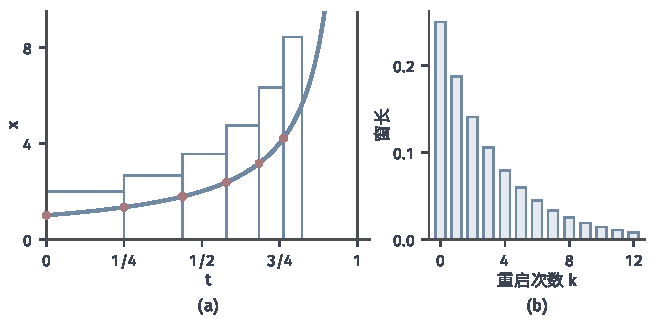
\includegraphics[width=112mm]{figures/06-differential-equations/01-ordinary-differential-equations/matplotlib/odeex-continuation-windows/figure.pdf}
  \caption{沿$\dot x=x^2$重启局部定理。(a)蓝线是真解，红点是重启点$(t_k,x_k)$，矩形是每次重启所用的时间窗$\delta_k$与状态范围$[0,2x_k]$，灰色竖线是$t=1$。(b)窗长$\delta_k=\tfrac14(3/4)^k$随重启次数按等比衰减，总和为$1$。}
  \label{fig:odeex-continuation-windows}
\end{BookInlineFigure}

这个例子提示了一般规律。时间窗只依赖盒子内的$M$和$L$。如果解始终留在一个固定的紧集内，$M,L$有共同的上界，窗口有一个不随重启变化的正下限，重启有限次就能越过任何有限时刻。所以解走不下去，只能是因为它没有留在任何紧集内。

\paragraph{紧集上的统一时间窗}
把这个想法写严格，需要两个引理：局部Lipschitz常数在紧集上可以取成统一的，局部定理的时间窗在紧集上也可以取成统一的。

\begin{lemma}[紧集上的统一Lipschitz常数]
\label{lem:odeex-compact-lipschitz}
设$\bm{K}\subseteq\bm{D}$是紧集。则存在常数$L$，使式~\eqref{eq:odeex-lipschitz}对$\bm{K}$中所有同一时刻的两点$(t,\bm{x}),(t,\bm{y})$成立。
\end{lemma}

\begin{proof}
设$M=\max_{\bm{K}}\lVert\bm{f}\rVert_2$。假设结论不成立，则对每个正整数$j$，存在$\bm{K}$中同一时刻的两点$(t_j,\bm{x}_j),(t_j,\bm{y}_j)$，使
\[
 \lVert\bm{f}(t_j,\bm{x}_j)-\bm{f}(t_j,\bm{y}_j)\rVert_2>j\lVert\bm{x}_j-\bm{y}_j\rVert_2.
\]
左端不超过$2M$，所以$\lVert\bm{x}_j-\bm{y}_j\rVert_2<2M/j\to0$。

由紧性，取子列使$(t_j,\bm{x}_j)$收敛到某点$(t_\ast,\bm{x}_\ast)\in\bm{K}$，此时$(t_j,\bm{y}_j)$也收敛到同一点。该点有定义~\ref{def:odeex-local-lipschitz}中的邻域和常数$L_\ast$，当$j$足够大时两点都在这个邻域内，不等号的左端不超过$L_\ast\lVert\bm{x}_j-\bm{y}_j\rVert_2$，再取$j>L_\ast$即得矛盾。
\end{proof}

\begin{lemma}[紧集上的统一时间窗]
\label{lem:odeex-uniform-window}
设$\bm{K}\subseteq\bm{D}$是紧集。则存在$\delta_{\bm{K}}>0$，使对每点$(s,\bm{\xi})\in\bm{K}$，以$(s,\bm{\xi})$为初值的问题在$[s-\delta_{\bm{K}},s+\delta_{\bm{K}}]$上有解。
\end{lemma}

\begin{proof}
若$\bm{D}$不是全空间，紧集$\bm{K}$到闭集$\bm{D}^{\mathrm{c}}$的距离大于零，取正数$\rho$小于这个距离的一半，否则取$\rho=1$。令
\[
 \bm{K}'=\bigl\{(t,\bm{x}):\exists(s,\bm{\xi})\in\bm{K},\ \lvert t-s\rvert\leq\rho/2,\ \lVert\bm{x}-\bm{\xi}\rVert_2\leq\rho/2\bigr\}.
\]
$\bm{K}'$是$\bm{K}$与一个紧盒子的和，因而紧，并且$\bm{K}'\subseteq\bm{D}$。

在$\bm{K}'$上取$M>0$为$\lVert\bm{f}\rVert_2$的上界，由引理~\ref{lem:odeex-compact-lipschitz}取$L>0$。对$\bm{K}$中任一点，$a=b=\rho/2$的盒子都含于$\bm{K}'$，定理~\ref{thm:odeex-picard-lindelof}给出共同的时间窗
\[
 \delta_{\bm{K}}=\min\Bigl\{\frac{\rho}{2},\frac{\rho}{2M},\frac{1}{2L}\Bigr\}.
\]
这就是所要的常数。
\end{proof}

\paragraph{离开每个紧集}
现在可以把“走不下去”说清楚。

\begin{theorem}[最大解离开紧集]
\label{thm:odeex-escape}
设$\bm{x}:(\omega_-,\omega_+)\to\mathbb{R}^{n}$是最大解。对每个紧集$\bm{K}\subseteq\bm{D}$，存在$t_{\bm{K}}\in(\omega_-,\omega_+)$，使当$t\in(t_{\bm{K}},\omega_+)$时，都有$(t,\bm{x}(t))\notin\bm{K}$。左端点$\omega_-$有对称的结论。
\end{theorem}

\begin{proof}
反设存在紧集$\bm{K}$和$t_j\uparrow\omega_+$，使$(t_j,\bm{x}(t_j))\in\bm{K}$。$\bm{K}$在时间方向有界，所以$\omega_+<+\infty$。

取引理~\ref{lem:odeex-uniform-window}中的$\delta_{\bm{K}}$，再取$j$使$t_j+\delta_{\bm{K}}>\omega_+$。以$(t_j,\bm{x}(t_j))$为初值的解$\bm{z}$在$[t_j-\delta_{\bm{K}},t_j+\delta_{\bm{K}}]$上存在，由引理~\ref{lem:odeex-common-uniqueness}，它在公共区间上与$\bm{x}$相同。

$\bm{z}$的定义区间越过了$\omega_+$，把$\bm{x}$与$\bm{z}$并起来就得到比最大解更长的解，矛盾。
\end{proof}

注意结论是“最终离开并且不再回来”，比“离开过”强。证明正是靠这一点：只要解在$\omega_+$附近回到$\bm{K}$一次，时间窗就能把它带过$\omega_+$。

\paragraph{两种障碍}
最常见的定义域是乘积形式$\bm{D}=J\times\bm{\Omega}$，其中$J$是右端给定的开时间区间，$\bm{\Omega}\subseteq\mathbb{R}^{n}$是开集。设$\omega_+<\sup J$，即解在右端还有定义的时候就停止了。对$\bm{\Omega}$的每个紧子集$\bm{C}$，$[t_0,\omega_+]\times\bm{C}$是$\bm{D}$的紧子集，由定理~\ref{thm:odeex-escape}，$\bm{x}(t)$在$\omega_+$之前最终离开$\bm{C}$。

特别地，状态空间是整个$\mathbb{R}^{n}$时，取$\bm{C}$为半径任意大的闭球，得到：若$\omega_+<\sup J$，则
\begin{equation}
 \lim_{t\uparrow\omega_+}\lVert\bm{x}(t)\rVert_2=+\infty.
 \label{eq:odeex-blowup-alternative}
\end{equation}
这就是有限时间爆炸。对一般的$\bm{\Omega}$，紧子集可以取成“离$\bm{\Omega}$的边界不太近且范数不太大”的集合，解要离开它们，要么范数趋于无穷，要么趋近$\bm{\Omega}$的边界，也可能在两者之间来回。

图~\ref{fig:odeex-exit-obstacles}给出三种典型情况，三个方程的右端都在各自定义域内满足本节的条件，$\omega_+=1$。

\begin{BookInlineFigure}
  \centering
  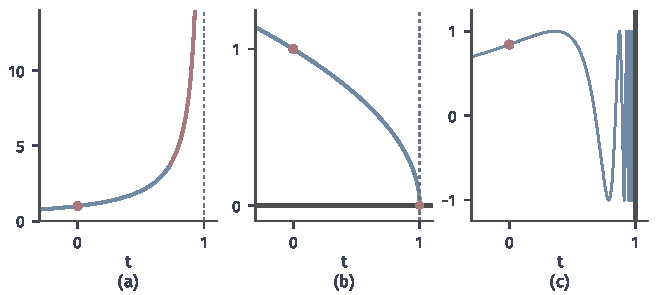
\includegraphics[width=112mm]{figures/06-differential-equations/01-ordinary-differential-equations/matplotlib/odeex-exit-obstacles/figure.pdf}
  \caption{最大解在$\omega_+=1$处结束的三种情形，红点是初值，灰色粗线是定义域的边界。(a)$\dot x=x^2$，$\bm{D}=\mathbb{R}^{2}$，状态趋于无穷（红色部分）。(b)$\dot x=-1/(2x)$，$\bm{D}=\mathbb{R}\times(0,\infty)$，解$\sqrt{1-t}$有界，趋近状态边界$x=0$。(c)$\bm{D}=(-\infty,1)\times\mathbb{R}$，解$\sin(1/(1-t))$有界且没有极限，时间到达定义域的边界$t=1$。}
  \label{fig:odeex-exit-obstacles}
\end{BookInlineFigure}

图(a)是状态无界的障碍：$\bm{\Omega}=\mathbb{R}$，解按式~\eqref{eq:odeex-blowup-alternative}趋于无穷。图(b)是逼近定义域边界的障碍：对$\dot x=-1/(2x)$，$x(0)=1$，由$(x^2)'=-1$得到$x=\sqrt{1-t}$，它在$t\uparrow1$时有界地趋于$0$，而$0$不在$\bm{\Omega}=(0,\infty)$中，右端在那里无定义，解不能再走。

图(c)是时间区间本身的端点：方程$\dot x=\cos\bigl(1/(1-t)\bigr)/(1-t)^2$，$x(0)=\sin1$的解是$\sin\bigl(1/(1-t)\bigr)$。此时$\omega_+=\sup J=1$，不属于式~\eqref{eq:odeex-blowup-alternative}的情形，定理~\ref{thm:odeex-escape}仍然成立，因为$(t,\bm{x}(t))$的时间分量趋向$\bm{D}$的边界。解有界但在$t\uparrow1$时没有极限，可见“离开紧集”不等于“收敛到某个边界点”。

\section{全局存在}
\label{sec:odeex-global}

状态空间是$\mathbb{R}^{n}$时，最大解只有一种走不到时间区间尽头的方式：范数趋于无穷。于是只要能预先证明解在任何有限时间段上有界，爆炸就被排除了，解会一直延续到右端给定的整个时间区间。这样的解称为\term{全局解}（global solution）。

\paragraph{爆炸快慢由增长速度决定}
先看标量自治方程，算出爆炸发生的时刻。设$f$在$[x_0,\infty)$上连续且为正，局部Lipschitz，解单调上升。由$\mathrm{d}t=\mathrm{d}x/f(x)$，走到无穷所需的时间是
\begin{equation}
 T=\int_{x_0}^{\infty}\frac{\mathrm{d}x}{f(x)}.
 \label{eq:odeex-blowup-time}
\end{equation}
这个积分有限时，解在$T$时刻爆炸；无穷时，解不爆炸。状态越大，箭头越快，走过单位状态所用的时间$1/f(x)$越短，这些时间加起来可能有限。

取$f(x)=x^p$，$x_0=1$。$p>1$时
\[
 T=\int_1^\infty x^{-p}\,\mathrm{d}x=\frac{1}{p-1},
\]
$p=2$时$T=1$，与前面的结果一致。$p=1$时积分发散，解是$\mathrm{e}^t$，增长虽快，但在有限时间内走不到无穷。线性增长正是这个分界线。图~\ref{fig:odeex-blowup-integral}(a)比较了$1/x^2$和$1/x$的尾部面积，图(b)比较了相应的解。

\begin{BookInlineFigure}
  \centering
  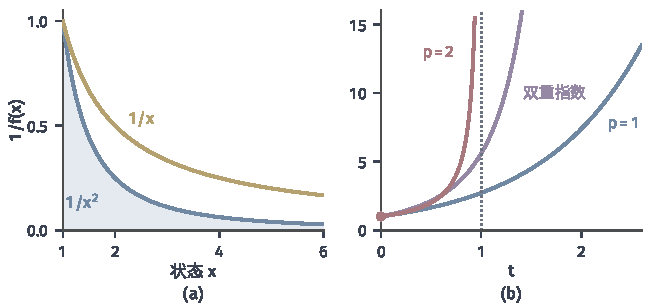
\includegraphics[width=112mm]{figures/06-differential-equations/01-ordinary-differential-equations/matplotlib/odeex-blowup-integral/figure.pdf}
  \caption{增长速度与有限时间爆炸。(a)走过单位状态的用时$1/f(x)$：蓝线$1/x^2$的尾部面积（浅蓝）有限，等于$1$；黄线$1/x$的尾部面积无穷。(b)初值都为$x(0)=1$的解：红线$\dot x=x^2$在$t=1$爆炸，蓝线$\dot x=x$是$\mathrm{e}^t$，紫线$\dot x=(1+x)\ln(1+x)$是$2^{\mathrm{e}^t}-1$，增长比线性快但不爆炸。}
  \label{fig:odeex-blowup-integral}
\end{BookInlineFigure}

\paragraph{至多线性增长}
线性增长是分界线，这一观察对向量方程仍然有用，只要把$\lVert\bm{f}\rVert_2$用状态范数的一次函数控制住。系数可以随时间变化，甚至只要局部可积。

\begin{theorem}[线性增长下的全局存在]
\label{thm:odeex-global}
设$J\subseteq\mathbb{R}$是开区间，$\bm{f}:J\times\mathbb{R}^{n}\to\mathbb{R}^{n}$连续，在状态方向局部Lipschitz连续且对时间局部一致。若存在$J$上局部可积的非负函数$\alpha,\beta$，使对所有$t\in J$，$\bm{x}\in\mathbb{R}^{n}$，
\begin{equation}
 \lVert\bm{f}(t,\bm{x})\rVert_2\leq\alpha(t)\lVert\bm{x}\rVert_2+\beta(t),
 \label{eq:odeex-linear-growth}
\end{equation}
则对每个$(t_0,\bm{x}_0)\in J\times\mathbb{R}^{n}$，最大解定义在整个$J$上，并且对$t\in J$，
\begin{equation}
 \lVert\bm{x}(t)\rVert_2\leq\Bigl(\lVert\bm{x}_0\rVert_2+\Bigl\lvert\int_{t_0}^{t}\beta\Bigr\rvert\Bigr)\exp\Bigl\lvert\int_{t_0}^{t}\alpha\Bigr\rvert.
 \label{eq:odeex-global-bound}
\end{equation}
\end{theorem}

满足式~\eqref{eq:odeex-linear-growth}的右端称为\term{至多线性增长}（at most linear growth）。证明分两步：先证明界~\eqref{eq:odeex-global-bound}，再用它排除爆炸。

\begin{proof}
设$\bm{x}$是最大解，定义在$(\omega_-,\omega_+)$上。先看$t\geq t_0$的一侧。取$T\in[t_0,\omega_+)$，记$u(t)=\lVert\bm{x}(t)\rVert_2$，它是$[t_0,T]$上的连续函数。由积分方程~\eqref{eq:odeex-integral}和式~\eqref{eq:odeex-linear-growth}，对$t\in[t_0,T]$，
\[
 u(t)\leq\lVert\bm{x}_0\rVert_2+\int_{t_0}^{t}\bigl(\alpha(s)u(s)+\beta(s)\bigr)\,\mathrm{d}s\leq B+\int_{t_0}^{t}\alpha(s)u(s)\,\mathrm{d}s,
\]
其中$B=\lVert\bm{x}_0\rVert_2+\int_{t_0}^{T}\beta$。

把右端记作$v(t)$，它在$[t_0,T]$上绝对连续，几乎处处有$\dot v=\alpha u\leq\alpha v$。令$A(t)=\int_{t_0}^t\alpha$，$A$也绝对连续。绝对连续函数的乘积仍绝对连续，于是几乎处处有
\[
 \frac{\mathrm{d}}{\mathrm{d}t}\bigl(v\,\mathrm{e}^{-A}\bigr)=(\dot v-\alpha v)\,\mathrm{e}^{-A}\leq0.
\]
绝对连续函数可由导数积分恢复，所以$v\,\mathrm{e}^{-A}$单调不增，由此
\[
 v(T)\leq v(t_0)\,\mathrm{e}^{A(T)}=B\,\mathrm{e}^{A(T)}.
\]
这里用到的绝对连续函数的性质，可参考\BookChapterRef{chap:integration}{卷四第6章“积分”}。由$u(T)\leq v(T)$，式~\eqref{eq:odeex-global-bound}在$t=T$处成立。

设$\omega_+<\sup J$。此时$[t_0,\omega_+]$是$J$的紧子集，$\alpha,\beta$在其上可积，所以式~\eqref{eq:odeex-global-bound}的右端对$T<\omega_+$有一个与$T$无关的上界。这与式~\eqref{eq:odeex-blowup-alternative}矛盾，于是$\omega_+=\sup J$。

$t\leq t_0$的一侧，令$\tilde{\bm{x}}(s)=\bm{x}(2t_0-s)$，它满足右端为$-\bm{f}(2t_0-s,\cdot)$的方程，增长条件的系数换成$\alpha(2t_0-s),\beta(2t_0-s)$，应用前面的结论即可。
\end{proof}

条件各有分工。式~\eqref{eq:odeex-linear-growth}是全局条件，要求对所有状态成立，正是它阻止了爆炸；Lipschitz条件只是局部的，它负责唯一性和最大解的存在，不参与防止爆炸。$\alpha,\beta$在紧时间段上可积，$\exp\int\alpha$才是有限数。

\paragraph{几个例子}
\begin{example}[线性系统]
\label{ex:odeex-linear-global}
设$\bm{A}(t)$和$\bm{g}(t)$在开区间$J$上连续，$\bm{f}(t,\bm{x})=\bm{A}(t)\bm{x}+\bm{g}(t)$。在紧时间段上$\lVert\bm{A}(t)\rVert_2$有界，
\[
 \lVert\bm{f}(t,\bm{x})-\bm{f}(t,\bm{y})\rVert_2\leq\lVert\bm{A}(t)\rVert_2\lVert\bm{x}-\bm{y}\rVert_2,
\]
满足局部Lipschitz条件。增长条件取$\alpha=\lVert\bm{A}(t)\rVert_2$，$\beta=\lVert\bm{g}(t)\rVert_2$，因此每个初值问题的解都定义在整个$J$上，这正是第~\ref{chap:linear-differential-systems}章的传播公式成立的范围。
\end{example}

\begin{example}[单摆]
\label{ex:odeex-pendulum-global}
单摆方程$\ddot x=-\sin x$写成状态$(x,v)$的系统，右端$\bm{f}(x,v)=(v,-\sin x)$是非线性的。由$\lvert\sin x\rvert\leq\lvert x\rvert$，
\[
 \lVert\bm{f}(x,v)\rVert_2=\sqrt{v^2+\sin^2x}\leq\lVert(x,v)\rVert_2.
\]
取$\alpha=1$，$\beta=0$，单摆的解对所有$t\in\mathbb{R}$存在，并满足
\[
 \lVert(x,v)(t)\rVert_2\leq\lVert(x_0,v_0)\rVert_2\,\mathrm{e}^{\lvert t\rvert}.
\]
\end{example}

\begin{example}[界与真解的比较]
\label{ex:odeex-barrier}
取$\dot x=\sqrt{1+x^2}$，$x(0)=0$，真解是$\sinh t$。由$\sqrt{1+x^2}\leq1+\lvert x\rvert$，可取$\alpha=\beta=1$，式~\eqref{eq:odeex-global-bound}给出，对$t\geq0$，
\[
 \lvert x(t)\rvert\leq t\,\mathrm{e}^{t}.
\]
在$t=1$处，界约为$2.718$，真解约为$1.175$。
\end{example}

图~\ref{fig:odeex-linear-growth-barrier}把这个界和真解画在一起，并与右端只多了平方项的$\dot x=1+x^2$对照。界比真解松得多，但它对每个有限的$t$都是有限数，这已足够排除爆炸；$\dot x=1+x^2$的解$\tan t$不满足线性增长条件，在$t=\pi/2$爆炸。

\begin{BookInlineFigure}
  \centering
  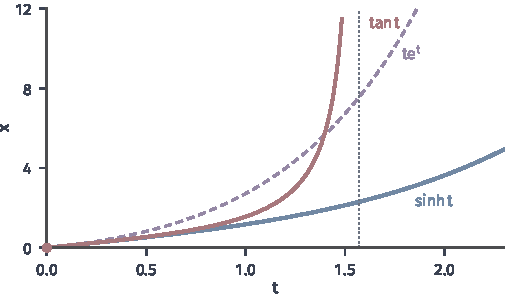
\includegraphics[width=88mm]{figures/06-differential-equations/01-ordinary-differential-equations/matplotlib/odeex-linear-growth-barrier/figure.pdf}
  \caption{线性增长下的上界。蓝线是$\dot x=\sqrt{1+x^2}$的解$\sinh t$，紫色虚线是由式~\eqref{eq:odeex-global-bound}得到的界$t\mathrm{e}^t$，红线是$\dot x=1+x^2$的解$\tan t$，在点线$t=\pi/2$处爆炸。初值都是$x(0)=0$。}
  \label{fig:odeex-linear-growth-barrier}
\end{BookInlineFigure}

\paragraph{条件的边界}
线性增长是充分条件，并不必要。前面图~\ref{fig:odeex-blowup-integral}(b)中的$\dot x=(1+x)\ln(1+x)$增长比线性快，令$y=\ln(1+x)$，方程化为$\dot y=y$，于是$x=2^{\mathrm{e}^t}-1$对所有$t$存在；由式~\eqref{eq:odeex-blowup-time}，这相当于$\int^{\infty}\mathrm{d}x/\bigl((1+x)\ln(1+x)\bigr)$发散。

符号也起作用。$\dot x=-x^3$的增长是三次的，但它把状态往零拉，解
\[
 x(t)=\frac{x_0}{\sqrt{1+2x_0^2t}}
\]
对所有$t\geq0$存在；向后走时，它在$t=-1/(2x_0^2)$爆炸。线性增长条件不看方向，所以它同时保证了两个时间方向的存在。

\paragraph{全局存在不是长期稳定}
定理~\ref{thm:odeex-global}只说解在每个有限时刻都有定义，不说解保持有界。$\dot x=x$的解$\mathrm{e}^t$全局存在，并趋于无穷；式~\eqref{eq:odeex-global-bound}的右端也随$t$增长。解的长期去向、是否靠近平衡点，要用另外的结构和条件来研究，可参考\BookChapterRef{chap:dynamical-systems-long-term}{卷九第1章“动力系统与轨迹的长期行为”}。

增长条件也不提供唯一性。式~\eqref{eq:odeex-sqrt}的右端满足$2\sqrt{\lvert x\rvert}\leq1+\lvert x\rvert$，是至多线性增长的，前面写出的解$x_c$对所有$t\geq0$都有定义，却有无穷多条。全局性与唯一性由不同的条件负责。

\section{时间可测的方程}
\label{sec:odeex-measurable}

前面的结论都要求右端对时间连续，但外部输入经常不连续。电路开关闭合、暖气切换功率时，输入在某些时刻跳变；更一般的输入可能只是一个可积函数。第~\ref{chap:ordinary-differential-equations}章已经看到，这类方程的解在跳变处有折角，不处处可微，要用积分方程来确定。对这样的右端，解的存在、唯一和延拓分别需要什么条件？

\paragraph{一个切换输入}
取$\dot x=-x+g(t)$，$x(0)=0$，其中$g(t)=1$（$0\leq t<1$），$g(t)=0$（$t\geq1$）。在$[0,1]$上解得
\[
 x(t)=1-\mathrm{e}^{-t},
\]
到$t=1$时$x(1)=1-\mathrm{e}^{-1}\approx0.632$。之后从这个值开始按齐次方程衰减，
\[
 x(t)=(1-\mathrm{e}^{-1})\,\mathrm{e}^{-(t-1)},\qquad t\geq1.
\]

两段在$t=1$处连续，但左导数是$\mathrm{e}^{-1}\approx0.368$，右导数是$-(1-\mathrm{e}^{-1})\approx-0.632$，如图~\ref{fig:odeex-measurable-switch}(b)。曲线处处满足积分方程，只在$t=1$这一点没有导数。

输入还可以无界。图~\ref{fig:odeex-measurable-switch}(c)的$\dot x=t^{-1/2}$，$x(0)=0$，在$t=0$处右端没有有限值，积分却收敛，解是$x=2\sqrt{t}$，在起点的切线是竖直的。把输入换成$1/t$就不行了：$\int_0^t\mathrm{d}s/s$发散，从$x(0)=0$出发的解不存在。可见起作用的不是有界性，而是右端在时间上可积。

\begin{BookInlineFigure}
  \centering
  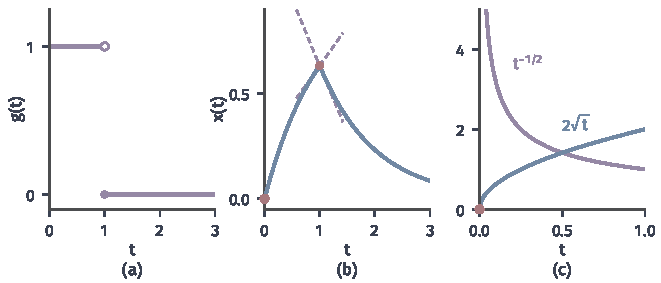
\includegraphics[width=112mm]{figures/06-differential-equations/01-ordinary-differential-equations/matplotlib/odeex-measurable-switch/figure.pdf}
  \caption{时间可测的右端。(a)切换输入$g$（紫线）。(b)$\dot x=-x+g(t)$，$x(0)=0$的解（蓝线），在$t=1$有折角，紫色虚线是左右两侧的切线。(c)无界但可积的输入$t^{-1/2}$（紫线）和解$2\sqrt{t}$（蓝线）。}
  \label{fig:odeex-measurable-switch}
\end{BookInlineFigure}

\paragraph{条件与解的定义}
把上面的观察写成条件。下面$J$是区间，$\bm{\Omega}\subseteq\mathbb{R}^{n}$是开集。

\begin{definition}[Carathéodory条件]
\label{def:odeex-caratheodory}
称$\bm{f}:J\times\bm{\Omega}\to\mathbb{R}^{n}$满足\term{Carathéodory条件}（Carathéodory conditions），是指：
\begin{enumerate}
 \item 对每个$\bm{x}\in\bm{\Omega}$，$t\mapsto\bm{f}(t,\bm{x})$是Lebesgue可测的；
 \item 对几乎每个$t\in J$，$\bm{x}\mapsto\bm{f}(t,\bm{x})$连续；
 \item 对每个紧区间$J'\subseteq J$和紧集$\bm{C}\subseteq\bm{\Omega}$，存在$m\in L^1(J')$，使对几乎每个$t\in J'$和所有$\bm{x}\in\bm{C}$，都有
 \begin{equation}
 \lVert\bm{f}(t,\bm{x})\rVert_2\leq m(t).
 \label{eq:odeex-caratheodory-bound}
 \end{equation}
\end{enumerate}
\end{definition}

第三条是局部可积的上界，它取代了连续函数在紧集上有界这件事。解的概念也要放宽。若$I\subseteq J$是含$t_0$的区间，$\bm{x}:I\to\bm{\Omega}$在每个紧子区间上绝对连续，$\bm{x}(t_0)=\bm{x}_0$，并且对几乎每个$t\in I$有$\dot{\bm{x}}(t)=\bm{f}(t,\bm{x}(t))$，就称$\bm{x}$是\term{Carathéodory解}（Carathéodory solution）。

绝对连续恰好使“几乎处处的导数”能积分回函数本身。因此这样的解就是满足积分方程~\eqref{eq:odeex-integral}的连续曲线，积分取Lebesgue意义。

绝对连续这一要求不能换成“连续且几乎处处满足方程”。图~\ref{fig:odeex-cantor-false}中的Cantor函数$c$在$[0,1]$上连续，几乎处处导数为零，并且$c(0)=0$。如果只看几乎处处的导数，$c$就满足$\dot x=0$，$x(0)=0$，唯一性立刻失败；但$c(1)=1$，积分方程的右端却恒为$0$，它不是Carathéodory解。

\begin{BookInlineFigure}
  \centering
  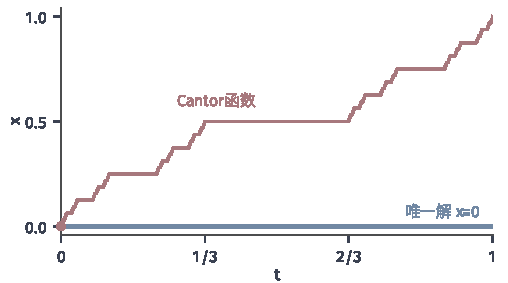
\includegraphics[width=86mm]{figures/06-differential-equations/01-ordinary-differential-equations/matplotlib/odeex-cantor-false/figure.pdf}
  \caption{绝对连续的必要性。方程是$\dot x=0$，$x(0)=0$，蓝线是它的唯一解$x\equiv0$。红线是Cantor函数，连续并几乎处处导数为零，但不绝对连续，不满足积分方程，因而不算解。}
  \label{fig:odeex-cantor-false}
\end{BookInlineFigure}

\paragraph{沿曲线的可测性}
积分方程要有意义，$s\mapsto\bm{f}(s,\bm{y}(s))$必须可测。条件只分别给出了对时间的可测性和对状态的连续性，下面的引理把两者合起来。

\begin{lemma}[沿连续曲线的可测性]
\label{lem:odeex-composition-measurable}
设$\bm{f}$满足定义~\ref{def:odeex-caratheodory}，$J'\subseteq J$是紧区间，$\bm{y}:J'\to\bm{C}$连续，$\bm{C}\subseteq\bm{\Omega}$紧。则$s\mapsto\bm{f}(s,\bm{y}(s))$在$J'$上可测，且可积。
\end{lemma}

\begin{proof}
把$J'$等分为$2^j$段，令$\bm{y}_j$在每段上取$\bm{y}$在该段左端点的值，右端点处取$\bm{y}$的值。在每段上$\bm{y}_j$是常向量，由条件1，$s\mapsto\bm{f}(s,\bm{y}_j(s))$在每段上可测，从而在$J'$上可测。

$\bm{y}$连续，所以$\bm{y}_j(s)\to\bm{y}(s)$对每个$s$成立。由条件2，对几乎每个$s$，$\bm{f}(s,\bm{y}_j(s))\to\bm{f}(s,\bm{y}(s))$。可测函数列的几乎处处极限可测，所以$\bm{f}(s,\bm{y}(s))$可测。可积性由式~\eqref{eq:odeex-caratheodory-bound}得到。
\end{proof}

\paragraph{局部存在}
Euler折线在这里不能用了。Euler格式需要右端在网格时刻$t_k$的值，而可测函数在单点的值没有意义，改变零测集上的值不改变方程，却能任意改变Euler格式。

替代办法是Tonelli的延迟逼近：用稍早一段的已知曲线计算积分，这样积分号里永远只含已经算好的部分，不需要逐点取值。

\begin{theorem}[Carathéodory存在定理]
\label{thm:odeex-caratheodory-existence}
设$\bm{f}$满足定义~\ref{def:odeex-caratheodory}，$[t_0,t_0+a]\subseteq J$，$\bm{B}_b\subseteq\bm{\Omega}$，$m\in L^1([t_0,t_0+a])$是$\bm{C}=\bm{B}_b$上的式~\eqref{eq:odeex-caratheodory-bound}的上界。取$\delta\in(0,a]$，使
\begin{equation}
 \int_{t_0}^{t_0+\delta}m(s)\,\mathrm{d}s\leq b.
 \label{eq:odeex-caratheodory-window}
\end{equation}
则初值问题在$[t_0,t_0+\delta]$上有取值于$\bm{B}_b$的Carathéodory解。$t_0$左侧有对称的结论。
\end{theorem}

积分$\int_{t_0}^{t_0+\delta}m$在$\delta\to0$时趋于零，满足式~\eqref{eq:odeex-caratheodory-window}的$\delta$总存在。它是$\delta\leq b/M$的自然推广：盒子的高度$b$现在由累计的速度上限来消耗。

\begin{proof}
\emph{延迟逼近。}记$I^+=[t_0,t_0+\delta]$，对正整数$N$，记$r=\delta/N$。定义$\bm{y}_N$：在$[t_0,t_0+r]$上$\bm{y}_N\equiv\bm{x}_0$；对$t\in(t_0+r,t_0+\delta]$，
\[
 \bm{y}_N(t)=\bm{x}_0+\int_{t_0}^{t-r}\bm{f}(s,\bm{y}_N(s))\,\mathrm{d}s.
\]
这个定义逐段进行：$t$在第$j+1$段时，积分只用到前$j$段上已定义的$\bm{y}_N$。由引理~\ref{lem:odeex-composition-measurable}，积分有定义。由式~\eqref{eq:odeex-caratheodory-window}，
\[
 \lVert\bm{y}_N(t)-\bm{x}_0\rVert_2\leq\int_{t_0}^{t-r}m(s)\,\mathrm{d}s\leq b,
\]
所以$\bm{y}_N$的取值都在$\bm{B}_b$中，递推能够继续。

\emph{等度连续。}令$W(\rho)$为$m$在$I^+$中长度不超过$\rho$的区间上积分的最大值。Lebesgue积分的绝对连续性给出$\rho\to0$时$W(\rho)\to0$。对$s<t$，$\bm{y}_N(t)-\bm{y}_N(s)$是一段长度不超过$t-s$的区间上的积分（或为零），所以
\[
 \lVert\bm{y}_N(t)-\bm{y}_N(s)\rVert_2\leq W(t-s).
\]
界$W$对所有$N$相同，$\{\bm{y}_N\}$一致有界且等度连续。由Arzelà--Ascoli判据，存在子列在$I^+$上一致收敛到连续曲线$\bm{x}:I^+\to\bm{B}_b$。

\emph{取极限。}把延迟积分写成到$t$的积分减去尾部，对所有$t\in I^+$（$t<t_0+r$时也成立）有
\[
 \bm{y}_N(t)=\bm{x}_0+\int_{t_0}^{t}\bm{f}(s,\bm{y}_N(s))\,\mathrm{d}s-\bm{E}_N(t),\qquad
 \lVert\bm{E}_N(t)\rVert_2\leq W(r).
\]
沿子列，$\bm{y}_N(s)\to\bm{x}(s)$，由条件2，对几乎每个$s$，$\bm{f}(s,\bm{y}_N(s))\to\bm{f}(s,\bm{x}(s))$。被积函数以$m$为可积控制，由控制收敛定理，积分收敛。尾部$\bm{E}_N$趋于零。

令$N\to\infty$，$\bm{x}$满足积分方程~\eqref{eq:odeex-integral}，因而是Carathéodory解。左侧用时间反演$s\mapsto2t_0-s$得到。
\end{proof}

图~\ref{fig:odeex-tonelli-delay}对切换输入的例子画出了延迟逼近。开头的一段$r$内曲线不动，因为积分尚未开始；之后曲线滞后真解一段时间，$N$增大时滞后变短，逐渐贴合真解。

\begin{BookInlineFigure}
  \centering
  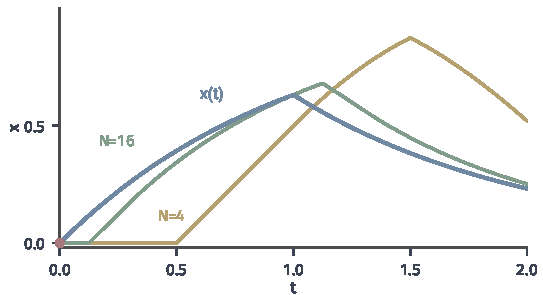
\includegraphics[width=92mm]{figures/06-differential-equations/01-ordinary-differential-equations/matplotlib/odeex-tonelli-delay/figure.pdf}
  \caption{延迟逼近。方程是$\dot x=-x+g(t)$，$x(0)=0$，$g$是图~\ref{fig:odeex-measurable-switch}(a)的切换输入，$\delta=2$。蓝线是解，黄线和绿线是$N=4$和$N=16$的延迟逼近$y_N$，延迟长度$r=\delta/N$。}
  \label{fig:odeex-tonelli-delay}
\end{BookInlineFigure}

\paragraph{唯一性}
存在定理对状态只要求连续，唯一性仍要另外的条件。第~\ref{sec:odeex-uniqueness}节的最后一个反例说明，对时间不一致的Lipschitz常数可以破坏唯一性；但$L$不必有界，可以放宽到$L$随时间局部可积。

\begin{theorem}[可积Lipschitz系数下的唯一性]
\label{thm:odeex-caratheodory-unique}
在定理~\ref{thm:odeex-caratheodory-existence}的记号下，设存在$\ell\in L^1([t_0,t_0+a])$，使对几乎每个$t\in[t_0,t_0+a]$和所有$\bm{x},\bm{y}\in\bm{B}_b$，
\begin{equation}
 \lVert\bm{f}(t,\bm{x})-\bm{f}(t,\bm{y})\rVert_2\leq\ell(t)\lVert\bm{x}-\bm{y}\rVert_2.
 \label{eq:odeex-integrable-lipschitz}
\end{equation}
取$\delta\in(0,a]$满足式~\eqref{eq:odeex-caratheodory-window}，以及
\begin{equation}
 \int_{t_0}^{t_0+\delta}\ell(s)\,\mathrm{d}s\leq\frac12.
 \label{eq:odeex-integrable-window}
\end{equation}
则初值问题在$[t_0,t_0+\delta]$上恰有一个取值于$\bm{B}_b$的Carathéodory解，Picard迭代~\eqref{eq:odeex-picard-iteration}一致收敛到它，并满足式~\eqref{eq:odeex-picard-error}。
\end{theorem}

\begin{proof}
证明与定理~\ref{thm:odeex-picard-lindelof}逐步对应。令$\mathcal{X}$为$[t_0,t_0+\delta]$上取值于$\bm{B}_b$的连续曲线组成的集合，它在一致距离下完备。

对$\bm{u}\in\mathcal{X}$，由引理~\ref{lem:odeex-composition-measurable}，$\mathcal{T}\bm{u}$有定义且连续，由式~\eqref{eq:odeex-caratheodory-window}，其取值在$\bm{B}_b$中。对$\bm{u},\bm{v}\in\mathcal{X}$，由式~\eqref{eq:odeex-integrable-lipschitz}和式~\eqref{eq:odeex-integrable-window}，
\[
 \lVert\mathcal{T}\bm{u}-\mathcal{T}\bm{v}\rVert_{\infty}
 \leq\int_{t_0}^{t_0+\delta}\ell(s)\lVert\bm{u}(s)-\bm{v}(s)\rVert_2\,\mathrm{d}s
 \leq\frac12\lVert\bm{u}-\bm{v}\rVert_{\infty}.
\]
由压缩映射定理得到唯一的不动点，它满足积分方程。取值于$\bm{B}_b$的Carathéodory解都是$\mathcal{T}$的不动点，所以都等于它。
\end{proof}

这里的压缩常数不再是“$L$乘时间”，而是系数的累计量$\int\ell$，后者由积分的绝对连续性保证在短时间内很小。一个解若从$\bm{x}_0$出发，由连续性在一小段时间内留在$\bm{B}_b$中，所以两条解在初始时刻重合后，局部总是相同的。

\begin{example}[系数无界的唯一性]
\label{ex:odeex-integrable-lipschitz}
考虑$\dot x=x/(2\sqrt{t})$，$x(0)=1$，取$b=1$。在$\lvert x-1\rvert\leq1$上，上界和Lipschitz系数分别可取
\[
 m(t)=\frac{1}{\sqrt{t}},\qquad\ell(t)=\frac{1}{2\sqrt{t}}.
\]
两者在$t\to0$时无界，但都可积。由$\int_0^\delta m=2\sqrt{\delta}$和$\int_0^\delta\ell=\sqrt{\delta}$，取$\delta=1/4$，式~\eqref{eq:odeex-caratheodory-window}和式~\eqref{eq:odeex-integrable-window}都成立。

从$x^{(0)}=1$出发迭代，第一步对$1/(2\sqrt{s})$积分，第二步对$(1+\sqrt{s})/(2\sqrt{s})$积分，分别得到
\[
 x^{(1)}=1+\sqrt{t},\qquad x^{(2)}=1+\sqrt{t}+\frac{t}{2}.
\]

一般地，$x^{(k)}=\sum_{j=0}^{k}(\sqrt{t})^j/j!$，极限是$\mathrm{e}^{\sqrt{t}}$。在$t=1/4$处，三轮迭代的取值依次是
\[
 1.5,\quad1.625,\quad1.6458,
\]
真解是$\mathrm{e}^{1/2}\approx1.6487$。
\end{example}

图~\ref{fig:odeex-integrable-lipschitz}比较了这个例子的系数与方程~\eqref{eq:odeex-clip}的系数。$1/(2\sqrt{t})$虽然也在原点无界，但其下的面积有限，短时间窗内的累计量可以小于$1/2$；$2/t$在原点附近的面积发散，没有任何时间窗能让累计量变小，多解正是从这里产生的。

\begin{BookInlineFigure}
  \centering
  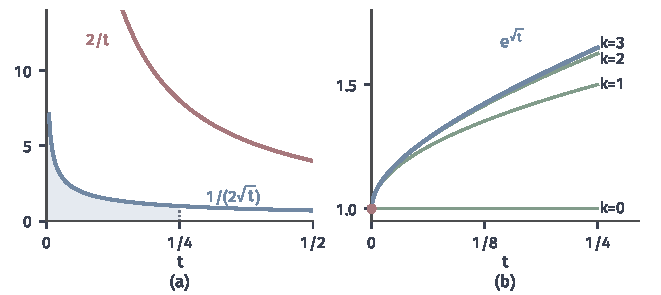
\includegraphics[width=112mm]{figures/06-differential-equations/01-ordinary-differential-equations/matplotlib/odeex-integrable-lipschitz/figure.pdf}
  \caption{时间上的Lipschitz系数。(a)蓝线$1/(2\sqrt{t})$可积，浅蓝面积是$[0,1/4]$上的累计量$1/2$；红线$2/t$在原点不可积。(b)$\dot x=x/(2\sqrt{t})$，$x(0)=1$的Picard迭代$x^{(0)},\ldots,x^{(3)}$（绿线）和解$\mathrm{e}^{\sqrt{t}}$（蓝线）。}
  \label{fig:odeex-integrable-lipschitz}
\end{BookInlineFigure}

\paragraph{唯一性不来自可测性或增长控制}
方程~\eqref{eq:odeex-sqrt}的右端满足Carathéodory条件，局部有界，并且至多线性增长，定理~\ref{thm:odeex-caratheodory-existence}保证它有解，但它有无穷多个解。时间可测性是对时间方向的放宽，增长控制处理的是解走多远，两者都不涉及两条解在状态方向上是否分开。方程~\eqref{eq:odeex-clip}也满足Carathéodory条件，它失败的原因是系数$2/t$不局部可积。

\paragraph{延拓与全局存在}
第~\ref{sec:odeex-maximal}节和第~\ref{sec:odeex-global}节的论证只用到积分方程，以及局部定理的时间窗在紧集上有统一下限，因此在下述条件下可以照搬：$\bm{f}$满足定义~\ref{def:odeex-caratheodory}，并且对每个紧区间$J'\subseteq J$和紧集$\bm{C}\subseteq\bm{\Omega}$，存在$\ell\in L^1(J')$，使式~\eqref{eq:odeex-integrable-lipschitz}在$J'\times\bm{C}$上成立。

唯一改动的地方是时间窗的选取。设$J$开，$\bm{K}\subseteq J\times\bm{\Omega}$紧，按引理~\ref{lem:odeex-uniform-window}的方式把$\bm{K}$放大成紧集，其上有共同的$m,\ell$。积分的绝对连续性给出一个$\delta_{\bm{K}}>0$，使$m$和$\ell$在任何长度不超过$\delta_{\bm{K}}$的时间段上的积分分别不超过$\rho/2$和$1/2$。

于是最大绝对连续解存在且唯一，最大存在区间在$J$中相对开，有限端点处解离开每个紧集。若增长条件~\eqref{eq:odeex-linear-growth}对几乎每个$t$成立，系数$\alpha,\beta$局部可积，定理~\ref{thm:odeex-global}及其上界~\eqref{eq:odeex-global-bound}也成立，因为那里的证明本来就只用了积分方程。切换输入的线性方程就属于这种情形，其解在整个时间轴上存在。

\section{流形上的局部解}
\label{sec:odeex-manifold}

球面上的风场、圆周上的匀速转动都是流形上的方程：未知量是流形上的一条曲线，右端是每点的切向量。流形没有全局的坐标，不能直接把上面的定理搬过去。办法是分两步：在一张坐标图内，方程就是欧氏空间的初值问题；跨图时，再用唯一性保证各张图上解出来的是同一条曲线。

\paragraph{坐标中的方程}
本节$M$是$n$维无边界光滑流形，$X$是$M$上的光滑向量场，流形、切向量与向量场的定义可参考\BookChapterRef{chap:manifold-basics}{卷四第24章“流形的基本概念”}。若可微曲线$\gamma:I\to M$对所有$t\in I$满足
\begin{equation}
 \dot\gamma(t)=X_{\gamma(t)},
 \label{eq:odeex-integral-curve}
\end{equation}
就称$\gamma$是$X$的\term{积分曲线}（integral curve）。

取坐标图$(U,\varphi)$，$X$在$U$上写成$X=\sum_iX_i\partial_i$。把分量读成坐标的函数，记
\[
 \bm{F}(\bm{x})=\bigl(X_1(\varphi^{-1}(\bm{x})),\ldots,X_n(\varphi^{-1}(\bm{x}))\bigr),\qquad\bm{x}\in\varphi(U).
\]
曲线的坐标记录$\bm{x}(t)=\varphi(\gamma(t))$的速度分量就是$\dot{\bm{x}}$，所以在$U$内，方程~\eqref{eq:odeex-integral-curve}等价于
\begin{equation}
 \dot{\bm{x}}=\bm{F}(\bm{x}).
 \label{eq:odeex-chart-equation}
\end{equation}
这是开集$\varphi(U)\subseteq\mathbb{R}^{n}$上的自治方程，右端光滑，第~\ref{sec:odeex-uniqueness}节的定理可用。

换一张图$(V,\psi)$，转移映射是$\tau=\psi\circ\varphi^{-1}$，同一条曲线的新记录是$\bm{y}=\tau(\bm{x})$。由链式法则，
\[
 \dot{\bm{y}}=\bm{J}_\tau(\bm{x})\dot{\bm{x}}=\bm{J}_\tau(\bm{x})\bm{F}(\bm{x}).
\]
切向量的分量按Jacobian矩阵变换，右端正好是$X$在新图中的分量$\bm{G}(\bm{y})$。因此$\bm{y}$满足新图中的方程$\dot{\bm{y}}=\bm{G}(\bm{y})$，两张图说的是同一件事，如图~\ref{fig:odeex-chart-transfer}。

\begin{BookInlineFigure}
  \centering
  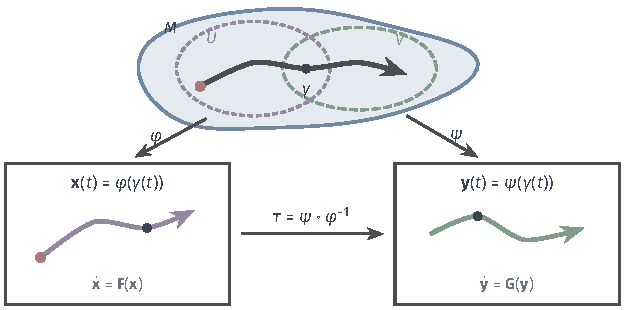
\includegraphics[width=106mm]{figures/06-differential-equations/01-ordinary-differential-equations/tikz/odeex-chart-transfer/figure.pdf}
  \caption{流形上的同一条积分曲线在两张坐标图中的记录。深灰曲线是$M$上的$\gamma$，紫色虚线和绿色虚线围成图的定义域$U,V$，下方是对应的坐标平面，曲线$\bm{x}$与$\bm{y}$分别满足各自的坐标方程。在重叠部分，黑点是同一个状态，转移映射$\tau$把一个方程变成另一个。}
  \label{fig:odeex-chart-transfer}
\end{BookInlineFigure}

\paragraph{局部解的拼接}
现在把第~\ref{sec:odeex-maximal}节的结论逐条搬到流形上。证明的结构不变，只是“盒子”换成坐标图内的盒子，距离的比较只在一张图内进行。

\begin{theorem}[积分曲线]
\label{thm:odeex-manifold}
设$M$是$n$维无边界光滑流形，$X$是其上的光滑向量场。
\begin{enumerate}
 \item 对每个$p\in M$，存在$\varepsilon>0$和积分曲线$\gamma:(-\varepsilon,\varepsilon)\to M$，使$\gamma(0)=p$。
 \item 若两条积分曲线定义在同一区间$I$上，且在某时刻取值相同，则它们在$I$上相同。
 \item 对每个$p\in M$，存在唯一的\term{最大积分曲线}（maximal integral curve）$\gamma_p:I_p\to M$，$\gamma_p(0)=p$，$I_p$是含$0$的开区间，以$p$为起点的积分曲线都是它的限制。
 \item 若$\omega_+=\sup I_p<+\infty$，则对$M$的每个紧子集$C$，存在$t_C\in I_p$，使当$t\in(t_C,\omega_+)$时$\gamma_p(t)\notin C$。
 \item 若$M$紧，则$I_p=\mathbb{R}$对每个$p$成立。
\end{enumerate}
\end{theorem}

\begin{proof}
\emph{结论1。}取含$p$的坐标图，在式~\eqref{eq:odeex-chart-equation}上应用定理~\ref{thm:odeex-picard-lindelof}，得到取值于$\varphi(U)$的解$\bm{x}$，令$\gamma=\varphi^{-1}\circ\bm{x}$。

\emph{结论2。}令$S=\{t\in I:\gamma_1(t)=\gamma_2(t)\}$，它非空。$M$是Hausdorff空间，$M\times M$的对角线闭，映射$t\mapsto(\gamma_1(t),\gamma_2(t))$连续，所以$S$在$I$中闭。

任取$t^\ast\in S$，取含$\gamma_1(t^\ast)$的坐标图$(U,\varphi)$。由连续性，$t^\ast$的某个邻域内两条曲线都留在$U$中，它们的坐标记录都解方程~\eqref{eq:odeex-chart-equation}并在$t^\ast$取相同的值，由定理~\ref{thm:odeex-picard-lindelof}重合。所以$S$在$I$中开，由连通性，$S=I$。

\emph{结论3。}与定理~\ref{thm:odeex-maximal}的证明相同：结论2使所有以$p$为起点的积分曲线相容，它们的并是最大积分曲线；若右端点属于$I_p$，从该点解局部问题就能再延长一段。

\emph{结论4。}先选有限覆盖。对每点$q\in C$取含它的坐标图及其内的一个紧邻域，$C$紧，所以有限个紧邻域$C_1,\ldots,C_r$覆盖$C$，各含于坐标图$(U_i,\varphi_i)$。对紧集$\{0\}\times\varphi_i(C_i)$应用引理~\ref{lem:odeex-uniform-window}，得到时间窗$\delta_i$，令$\delta=\min_i\delta_i$。从$C$的任一点出发的积分曲线至少存在时间$\delta$。

反设存在$t_j\uparrow\omega_+$使$\gamma_p(t_j)\in C$，取$j$使$t_j+\delta>\omega_+$。$X$不显含时间，所以从$\gamma_p(t_j)$出发、再走时间$\delta$的积分曲线平移后接在$\gamma_p$之后，由结论2相容，它越过了$\omega_+$，矛盾。

\emph{结论5。}取$C=M$，$\gamma_p(t)$不可能离开$M$，由结论4，$\sup I_p=+\infty$；对$-X$同样推理，$\inf I_p=-\infty$。
\end{proof}

结论2用到了流形定义中的Hausdorff条件，局部的Picard定理本身用不上它。在双原点直线上取向量场$\partial_x$，从$x=-1$出发的积分曲线到$t=1$时可以到达任一个原点：两条积分曲线在$t<1$时重合，在$t=1$时不同，局部唯一性并不能排除这一点。流形的定义排除了这种空间。满足结论5的向量场称为\term{完备向量场}（complete vector field）。

\paragraph{图内爆炸不是流形上爆炸}
定理~\ref{thm:odeex-escape}用在坐标方程上时，说的是解离开$\varphi(U)$的紧子集，这可能只是走出了这张图。单位圆$S^1$上的匀速转动是最简单的例子。

设$\bm{y}=(\sin\alpha,-\cos\alpha)$，$\alpha=0$是南极，$\alpha=\pi$是北极。令向量场使$\dot\alpha=2$。取从北极出发的球极投影作图：$u=y_1/(1-y_2)$，定义域是$S^1$去掉北极，代入得到$u=\tan(\alpha/2)$。求导，$X$在这张图中的方程是
\[
 \dot u=\frac{1}{2\cos^2(\alpha/2)}\dot\alpha=1+u^2.
\]

从南极出发，$u(0)=0$，解是$u=\tan t$，在$t=\pi/2$时趋于无穷。这与$\dot x=1+x^2$的爆炸是同一个公式，但这里的$u\to\infty$只意味着曲线走向北极，也就是走出了这张图。

换用从南极出发的投影$v=y_1/(1+y_2)$，定义域是$S^1$去掉南极。转移映射是$v=1/u$，所以新图中的方程为
\[
 \dot v=-\frac{\dot u}{u^2}=-\frac{1+u^2}{u^2}=-(1+v^2).
\]
在$t=\pi/4$时，$u=1$，$v=1$。从这里在第二张图中继续解，得到$v=\cot t$，它在$t=\pi/2$时取值$0$，平稳地经过北极。图~\ref{fig:odeex-chart-blowup}显示了这次换图。

\begin{BookInlineFigure}
  \centering
  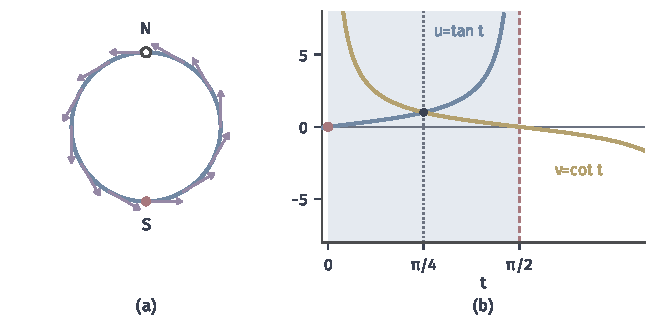
\includegraphics[width=112mm]{figures/06-differential-equations/01-ordinary-differential-equations/matplotlib/odeex-chart-blowup/figure.pdf}
  \caption{图内爆炸不是流形上爆炸。(a)单位圆上的匀速旋转场（紫色箭头），红点是南极$S$，空心点是第一张图未覆盖的北极$N$。(b)蓝线是第一张图的坐标$u=\tan t$，在红色虚线$t=\pi/2$爆炸；黄线是第二张图的坐标$v=\cot t$，在该处取值$0$。黑点是$t=\pi/4$处的换图点，$u=v=1$。}
  \label{fig:odeex-chart-blowup}
\end{BookInlineFigure}

圆是紧流形，由定理~\ref{thm:odeex-manifold}的结论5，积分曲线对所有$t$存在，这里$\alpha=2t$确实如此。

\paragraph{嵌入流形上的切向量场}
流形常常作为$\mathbb{R}^{N}$中的约束集合出现。设$M\subseteq\mathbb{R}^{N}$是嵌入子流形，$W\supseteq M$是开集，$\tilde{\bm{f}}:W\to\mathbb{R}^{N}$光滑，并且在$M$上切于$M$，即$\tilde{\bm{f}}(\bm{p})\in T_{\bm{p}}M$。我们希望知道，从$M$上出发解环境方程$\dot{\bm{y}}=\tilde{\bm{f}}(\bm{y})$，解是否留在$M$上。

唯一性给出的回答很简洁。$\tilde{\bm{f}}$限制在$M$上是$M$的向量场，由定理~\ref{thm:odeex-manifold}有$M$内的积分曲线$\gamma$。把$\gamma$看成$\mathbb{R}^{N}$中的曲线，它就是环境方程的解。环境方程的解是唯一的，所以环境解在$\gamma$存在的时间段内就是$\gamma$，它留在$M$上。约束不需要在算法上另外施加，切向条件加唯一性就够了。

\begin{example}[球面上的旋转场]
\label{ex:odeex-sphere-rotation}
在$\mathbb{R}^{3}$中取$\tilde{\bm{f}}(\bm{y})=(-y_2,y_1,0)$。对$\bm{y}\in S^2$，有$\langle\bm{y},\tilde{\bm{f}}(\bm{y})\rangle=0$，场切于球面。环境方程是线性的，解为绕竖直轴的旋转，保持$\lVert\bm{y}\rVert_2=1$。把$\tilde{\bm{f}}$换成不切的场$(1,0,0)$，解$\bm{y}_0+t(1,0,0)$立即离开球面。
\end{example}

\paragraph{测地线的初值问题}
黎曼流形$(M,g)$上的测地线方程在坐标中写作
\begin{equation}
 \ddot x_k+\sum_{i,j}\Gamma^k_{i,j}(\bm{x})\,\dot x_i\dot x_j=0,\qquad k=1,\ldots,n.
 \label{eq:odeex-geodesic}
\end{equation}
相关的定义可参考\BookChapterRef{chap:riemannian-geometry}{卷四第27章“黎曼几何”}。那里陈述并使用了光滑方程的局部理论，局部存在唯一、最大解和离开紧集三项在这一节得到了证明，光滑依赖由第~\ref{chap:ode-sensitivity}章证明。

它是二阶方程，状态要包括位置和速度。令$\bm{w}=\dot{\bm{x}}$，得到一阶系统
\[
 \dot{\bm{x}}=\bm{w},\qquad\dot w_k=-\sum_{i,j}\Gamma^k_{i,j}(\bm{x})\,w_iw_j.
\]
右端在$\varphi(U)\times\mathbb{R}^{n}$上光滑，定理~\ref{thm:odeex-picard-lindelof}给出局部解。全体$(p,\bm{w})$（$p\in M$，$\bm{w}\in T_pM$）组成的集合称为\term{切丛}（tangent bundle），记为$TM$，它是$2n$维流形，$(\bm{x},\bm{w})$是其坐标。

测地线就是$TM$上一个向量场的积分曲线在$M$上的投影。条件$D\dot\gamma/\mathrm{d}t=0$不依赖坐标，所以不同的图给出的是同一条曲线，定理~\ref{thm:odeex-manifold}的结论都适用：每个初始位置和初始速度决定唯一的最大测地线。

速度的长度沿测地线不变，这给出了$M$紧时的整体结论。设$M$紧，$\lVert\dot\gamma\rVert_g$恒等于初始速度的长度$c$，于是$(\gamma,\dot\gamma)$始终留在集合$\{(p,\bm{w})\in TM:g_p(\bm{w},\bm{w})=c^2\}$中，这个集合是紧的。由结论4，测地线对所有$t$存在。

球面上还可以把测地线写成环境方程，直接看约束是如何保持的。$S^2\subset\mathbb{R}^{3}$的测地线加速度沿法向，方程是
\begin{equation}
 \ddot{\bm{y}}=-\lVert\dot{\bm{y}}\rVert_2^2\,\bm{y}.
 \label{eq:odeex-sphere-geodesic}
\end{equation}
右端是$(\bm{y},\dot{\bm{y}})\in\mathbb{R}^{6}$的光滑函数，在$\mathbb{R}^{3}$中到处都有定义。设初值满足$\lVert\bm{y}(0)\rVert_2=1$和$\langle\bm{y}(0),\dot{\bm{y}}(0)\rangle=0$。

令$c=\lVert\bm{y}\rVert_2^2-1$，$d=\langle\bm{y},\dot{\bm{y}}\rangle$，它们衡量解偏离约束的程度。由式~\eqref{eq:odeex-sphere-geodesic}，
\[
 \dot c=2d,\qquad\dot d=\lVert\dot{\bm{y}}\rVert_2^2+\langle\bm{y},\ddot{\bm{y}}\rangle=-\lVert\dot{\bm{y}}\rVert_2^2\,c.
\]
沿给定的解，$\lVert\dot{\bm{y}}(t)\rVert_2^2$是已知的连续函数，这是关于$(c,d)$的线性系统，初值为零。由唯一性，$(c,d)\equiv\bm{0}$，解永远留在球面上，速度永远切于球面。

取$\bm{p}=(1,0,0)$，$\bm{v}=(0,1,0)$，解是赤道$\bm{y}(t)=(\cos t,\sin t,0)$，此时$\lVert\dot{\bm{y}}\rVert_2^2=1$，$\ddot{\bm{y}}=-\bm{y}$，方程成立。图~\ref{fig:odeex-sphere-constraint}(b)中的蓝线是数值积分得到的$\lVert\bm{y}\rVert_2^2-1$，保持为零。

若初速度不切于球面，例如$\bm{v}=(0.25,1,0)$，则$(c,d)$的初值不为零，$c$随时间偏离零，图中红线的最大值约为$0.39$。约束是否保持，完全取决于初值是否在约束集合上，这正是唯一性的结论。

\begin{BookInlineFigure}
  \centering
  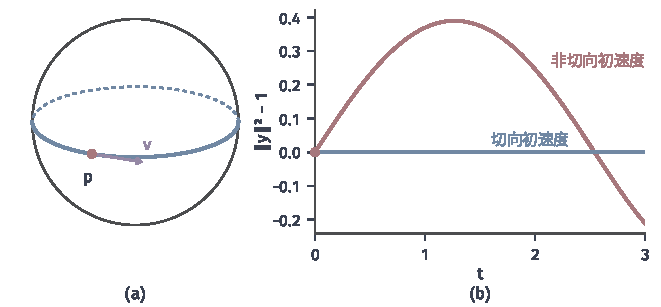
\includegraphics[width=112mm]{figures/06-differential-equations/01-ordinary-differential-equations/matplotlib/odeex-sphere-constraint/figure.pdf}
  \caption{球面测地线的环境方程~\eqref{eq:odeex-sphere-geodesic}。(a)单位球面上过红点$\bm{p}$、初速度为紫色箭头$\bm{v}$的测地线（赤道，背面用虚线）。(b)约束偏差$\lVert\bm{y}\rVert_2^2-1$：蓝线是切向初速度$(0,1,0)$，恒为零；红线是非切向初速度$(0.25,1,0)$，解离开球面。}
  \label{fig:odeex-sphere-constraint}
\end{BookInlineFigure}

平行移动方程
\[
 \dot V_k+\sum_{i,j}\Gamma^k_{i,j}(\bm{x}(t))\,\dot x_iV_j=0
\]
是关于$V$的线性方程，系数沿给定曲线连续。由例~\ref{ex:odeex-linear-global}，它在曲线的整个定义区间上有唯一解，跨图时由唯一性分段接续。测地线方程则是速度的二次方程，局部解未必能延伸到所有时间，这与开单位球上直线走到边界的情形一致，也正是定理~\ref{thm:odeex-escape}所说的状况。

\section{本章小结}
\label{sec:odeex-summary}

章首的三个方程分别暴露了三个问题：$\dot x=x^2$在有限时间内走不下去，$\dot x=2\sqrt{\lvert x\rvert}$有多条解，右端跳变的方程从零点出发无解。本章逐一给出了这些问题的条件，图~\ref{fig:odeex-summary-map}把它们串在一起。

局部存在只回答“有没有解”。有限维空间中右端连续就够了：Euler折线被关在盒子内，紧性抽出收敛的子列，连续性让极限满足方程。这条路线只给出一个解，子列的选择甚至依赖扰动，在无限维空间也可能失败。

唯一性回答“解是否由初值确定”。状态方向的局部Lipschitz条件使积分映射在短时间窗内成为压缩映射，靠完备性而不是紧性得到不动点，存在、唯一和迭代误差界同时得到。这一条件是便于验证的充分条件，单调性也能给出单向的唯一性；但Lipschitz常数对时间不局部可积时，唯一性可以失败。

\begin{BookInlineFigure}
  \centering
  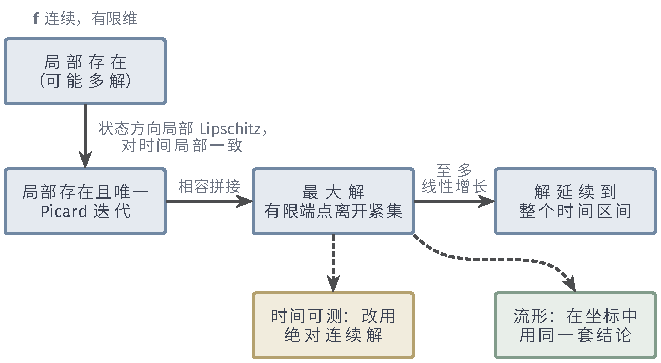
\includegraphics[width=112mm]{figures/06-differential-equations/01-ordinary-differential-equations/tikz/odeex-summary-map/figure.pdf}
  \caption{本章结论的依赖关系。从连续右端的局部存在出发，加上状态方向的局部Lipschitz条件得到局部存在且唯一，相容拼接得到最大解，至多线性增长使解延续到整个时间区间。虚线表示同一链条的两个推广：时间可测的方程和流形上的方程。}
  \label{fig:odeex-summary-map}
\end{BookInlineFigure}

最大延拓回答“局部解能接多长”。唯一性使局部解相容，并成唯一的最大解。解的定义区间是开区间，到有限端点时解离开定义域的每个紧集，表现为状态无界或趋近定义域的边界。全局存在回答“解能否走完给定的时间区间”，至多线性增长的右端保证了这一点，但解仍可能无界，全局存在也不提供唯一性。表~\ref{tab:odeex-summary}按问题列出了条件和反例。

\begin{BookInlineTable}
  \centering
  \caption{各问题的条件与反例}
  \label{tab:odeex-summary}
  \begin{tabularx}{\linewidth}{lXX}
    \toprule
    问题 & 条件（$\bm{f}$连续时） & 去掉条件的反例 \\
    \midrule
    局部存在 & 有限维，$\bm{f}$连续 & 右端跳变无解；$c_0$上连续而无解 \\
    唯一性 & 状态方向局部Lipschitz，对时间局部一致 & $2\sqrt{\lvert x\rvert}$的漏斗；系数$2/t$ \\
    最大延拓 & 局部存在且唯一 & 没有唯一性时最大解不唯一 \\
    全局存在 & 至多线性增长 & $\dot x=x^2$在$t=1$爆炸 \\
    \bottomrule
  \end{tabularx}
\end{BookInlineTable}

时间可测时，解要换成绝对连续解，对应的条件是：对时间可测、对状态连续、局部可积上界，由此得到存在；唯一性另要求状态方向的Lipschitz系数对时间局部可积，这不能由可测性或增长控制推出。这些结论只针对满足积分方程的绝对连续曲线，连续且几乎处处满足方程还不够，Cantor函数就是反例。

流形上，局部存在唯一性在每张坐标图内应用，切向量的变换规律使不同的图描述同一条曲线，Hausdorff条件和唯一性把它们接成最大积分曲线。坐标方程的爆炸可能只是走出了一张图，紧流形上的积分曲线对所有时间存在。切向条件和唯一性共同使解保持在流形上，测地线方程是这一结构的代表。

这些结论都只说明解的存在、唯一和存在区间，是有限时间上的定性结论。解对初值和参数怎样变化，变化能否求导，由第~\ref{chap:ode-sensitivity}章在这里的存在性保证上继续建立；第~\ref{chap:ode-numerical-methods}章的数值方法也是在解存在且唯一时才有明确的逼近目标。


\chapter{解的敏感性}
\label{chap:ode-sensitivity}

培养液里细菌的相对密度满足$\dot{x}=x(1-x)$。若初始密度测得$x(0)=1/4$，解是
\[
 x(t)=\frac{x_0\mathrm{e}^{t}}{1-x_0+x_0\mathrm{e}^{t}},\qquad x_0=\frac14,
\]
在$t=\ln3$时$x=1/2$。可是初始密度带有测量误差，增长率也只是估计值。把$x_0$改成$0.26$，$t=\ln3$时的值会差多少？把增长率改$20\%$呢？第~\ref{chap:ode-existence-continuation}章保证了解存在且唯一，却没有回答这些问题。

大多数方程写不出解的公式，因此我们要在不解方程的情况下回答它们。回答有三种精度。最粗的是整段曲线的差不超过多少，这只需要估计，由Gronwall不等式完成。其次是一阶响应：初值或参数沿某方向变一点，解沿哪个方向变、变多少，这要先证明解可微，再解一个线性方程。最后，若关心的只是由解算出的一个目标值，而参数很多，就用一次反向求解得到全部偏导数。

本章按这三种精度展开。Gronwall估计给出曲线距离的上界，并依次用于初值、参数和输入的改变。变分方程给出一阶响应。把初始状态到后续状态的关系看成映射，就得到流映射，它的Jacobian矩阵回答小区域的拉伸和体积变化，Hamilton流是其中保持体积的一类。最后由变分方程导出伴随方程。全章只讨论有限时间区间上的结论，上面的方程$\dot{x}=x(1-x)$会反复用作手算的例子。

\section{Gronwall估计}
\label{sec:odesens-gronwall}

没有解的公式，怎样比较两条解曲线？回到积分形式。解是右端的累积，两条解的差也就是右端之差的累积，而右端之差又可以由解的差控制。这样得到一个把未知量放在两边的不等式，Gronwall不等式负责把它解开。

\paragraph{两条积分方程相减}
设$\bm{x}$和$\bm{y}$在$[t_0,T]$上绝对连续，分别满足
\[
 \dot{\bm{x}}=\bm{f}(t,\bm{x}),\qquad
 \dot{\bm{y}}=\bm{f}(t,\bm{y})+\bm{r}(t),
\]
初值为$\bm{x}(t_0)=\bm{x}_0$，$\bm{y}(t_0)=\bm{y}_0$，方程几乎处处成立。这里$\bm{r}(t)$是第二条曲线相对于方程的\term{残差}（residual），表示每一时刻额外多出来的变化率。写成积分形式，
\[
 \begin{aligned}
 \bm{x}(t)&=\bm{x}_0+\int_{t_0}^{t}\bm{f}(s,\bm{x}(s))\,\mathrm{d}s,\\
 \bm{y}(t)&=\bm{y}_0+\int_{t_0}^{t}\bigl[\bm{f}(s,\bm{y}(s))+\bm{r}(s)\bigr]\,\mathrm{d}s.
 \end{aligned}
\]
记$\bm{e}(t)=\bm{y}(t)-\bm{x}(t)$，$\bm{e}_0=\bm{y}_0-\bm{x}_0$。两式相减，得到
\[
 \bm{e}(t)=\bm{e}_0+\int_{t_0}^{t}\bigl[\bm{f}(s,\bm{y}(s))-\bm{f}(s,\bm{x}(s))\bigr]\,\mathrm{d}s+\int_{t_0}^{t}\bm{r}(s)\,\mathrm{d}s.
\]

现在设右端关于状态满足Lipschitz条件，在时刻$s$的常数为$L(s)$，也就是
\[
 \lVert\bm{f}(s,\bm{y}(s))-\bm{f}(s,\bm{x}(s))\rVert_2\leq L(s)\lVert\bm{e}(s)\rVert_2.
\]
取范数并用三角不等式，$u(t)=\lVert\bm{e}(t)\rVert_2$满足
\begin{equation}
 u(t)\leq\lVert\bm{e}_0\rVert_2+\int_{t_0}^{t}\bigl[L(s)u(s)+\lVert\bm{r}(s)\rVert_2\bigr]\,\mathrm{d}s.
 \label{eq:odesens-error-inequality}
\end{equation}
式~\eqref{eq:odesens-error-inequality}两边都有$u$，并没有给出$u$的上界：要知道今天的误差，得先知道过去的误差。

\paragraph{复利的图景}
把$u$看成账户余额，$L(s)$是时刻$s$的利率，$\lVert\bm{r}(s)\rVert_2$是时刻$s$的存款速度，$\lVert\bm{e}_0\rVert_2$是本金。一小段时间$h$内，余额至多变成
\[
 u(s+h)\lesssim\bigl(1+L(s)h\bigr)u(s)+\lVert\bm{r}(s)\rVert_2h.
\]
这正是复利的递推。复利的结果可以直接写出：本金从$t_0$起计息，到$t$时乘以$\exp\int_{t_0}^{t}L$；时刻$s$存入的一小笔钱只从$s$起计息，到$t$时乘以$\exp\int_{s}^{t}L$。

图~\ref{fig:odesens-gronwall-deposits}画出了这两种钱的去向。类比也有限度：账户的利率真实发生，而式~\eqref{eq:odesens-error-inequality}只说误差“至多”按这个利率增长，真实的误差可能增长得慢，甚至缩小。Gronwall不等式给出的因此只是上界。

\begin{BookInlineFigure}
  \centering
  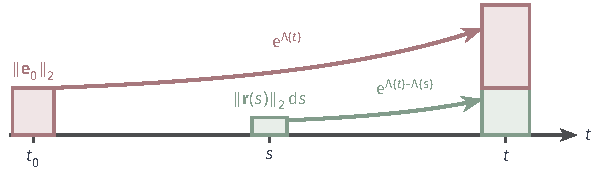
\includegraphics[width=101.9mm]{figures/06-differential-equations/01-ordinary-differential-equations/tikz/odesens-gronwall-deposits/figure.pdf}
  \caption{误差的复利账本示意。红色是初值误差$\lVert\bm{e}_0\rVert_2$，从$t_0$起一直被放大；绿色是时刻$s$处残差新注入的一小笔$\lVert\bm{r}(s)\rVert_2\,\mathrm{d}s$，只经历$s$之后的放大。时刻$t$的总上界是所有这些量放大后的和。}
  \label{fig:odesens-gronwall-deposits}
\end{BookInlineFigure}

\paragraph{Gronwall不等式}
复利的结论对一切满足该积分不等式的函数都成立，这就是\term{Gronwall不等式}（Gronwall inequality）。为了同时适用于可测输入，放大系数只要求可积。

\begin{lemma}[Gronwall不等式]
\label{lem:odesens-gronwall}
设$u:[t_0,T]\to[0,\infty)$连续，$a\geq0$是常数，$\beta,b:[t_0,T]\to[0,\infty)$可积，且对每个$t\in[t_0,T]$，
\begin{equation}
 u(t)\leq a+\int_{t_0}^{t}\bigl[\beta(s)u(s)+b(s)\bigr]\,\mathrm{d}s.
 \label{eq:odesens-gronwall-hypothesis}
\end{equation}
记$\Lambda(t)=\int_{t_0}^{t}\beta(s)\,\mathrm{d}s$。则对每个$t\in[t_0,T]$，
\begin{equation}
 u(t)\leq a\,\mathrm{e}^{\Lambda(t)}+\int_{t_0}^{t}\mathrm{e}^{\Lambda(t)-\Lambda(s)}b(s)\,\mathrm{d}s.
 \label{eq:odesens-gronwall-conclusion}
\end{equation}
\end{lemma}

\begin{proof}
记式~\eqref{eq:odesens-gronwall-hypothesis}的右端为$w(t)$。$\beta u+b$可积，所以$w$绝对连续，且几乎处处有
\[
 \dot{w}=\beta u+b.
\]
因为$\beta\geq0$，把$u\leq w$代入，得到
\[
 \dot{w}\leq\beta w+b.
\]

这是一阶线性不等式，用积分因子$\mathrm{e}^{-\Lambda}$处理。$\Lambda$绝对连续，两个绝对连续函数的乘积也绝对连续，于是几乎处处有
\[
 \frac{\mathrm{d}}{\mathrm{d}t}\bigl(\mathrm{e}^{-\Lambda}w\bigr)=\mathrm{e}^{-\Lambda}(\dot{w}-\beta w)\leq\mathrm{e}^{-\Lambda}b.
\]

从$t_0$到$t$积分，并用$w(t_0)=a$、$\Lambda(t_0)=0$，得到
\[
 \mathrm{e}^{-\Lambda(t)}w(t)\leq a+\int_{t_0}^{t}\mathrm{e}^{-\Lambda(s)}b(s)\,\mathrm{d}s.
\]
两边乘以$\mathrm{e}^{\Lambda(t)}$，再用$u\leq w$，就是式~\eqref{eq:odesens-gronwall-conclusion}。
\end{proof}

证明里$\beta\geq0$只用了一次，却不能省：把$u$放大成$w$再乘以$\beta$，不等号的方向要靠$\beta$非负。取$\beta\equiv-1$、$a=1$、$b=0$，定义
\[
 u(t)=\min\bigl\{\max\{t-1,0\},\,1/4\bigr\},\qquad t\in[0,3].
\]
它不超过$1/4$，积分$\int_0^3u$等于$15/32$，所以$1-\int_0^tu\geq17/32\geq u(t)$，假设式成立。若结论式仍成立，应有$u(3)\leq\mathrm{e}^{-3}\approx0.05$，而实际$u(3)=1/4$。负的放大率要换用微分形式处理，第~\ref{sec:odesens-initial}节会回到这一点。

\paragraph{基本误差估计}
把引理用于式~\eqref{eq:odesens-error-inequality}，就得到本章反复使用的比较定理。定理只要求两条曲线所经过的集合上有Lipschitz常数，这个集合怎样选取留给下一节。

\begin{theorem}[基本误差估计]
\label{thm:odesens-basic-estimate}
设$\bm{K}\subseteq\mathbb{R}^{n}$，曲线$\bm{x},\bm{y}:[t_0,T]\to\bm{K}$绝对连续，几乎处处满足$\dot{\bm{x}}=\bm{f}(t,\bm{x})$与$\dot{\bm{y}}=\bm{f}(t,\bm{y})+\bm{r}(t)$，其中$\bm{r}$可积。设存在可积函数$L\geq0$，使对几乎每个$t$及所有$\bm{a},\bm{b}\in\bm{K}$，
\begin{equation}
 \lVert\bm{f}(t,\bm{a})-\bm{f}(t,\bm{b})\rVert_2\leq L(t)\lVert\bm{a}-\bm{b}\rVert_2.
 \label{eq:odesens-lipschitz}
\end{equation}
记$\Lambda(t)=\int_{t_0}^{t}L(s)\,\mathrm{d}s$。则对每个$t\in[t_0,T]$，
\begin{equation}
 \lVert\bm{y}(t)-\bm{x}(t)\rVert_2\leq\mathrm{e}^{\Lambda(t)}\lVert\bm{y}_0-\bm{x}_0\rVert_2+\int_{t_0}^{t}\mathrm{e}^{\Lambda(t)-\Lambda(s)}\lVert\bm{r}(s)\rVert_2\,\mathrm{d}s.
 \label{eq:odesens-basic-estimate}
\end{equation}
\end{theorem}

\begin{proof}
由式~\eqref{eq:odesens-lipschitz}，$u=\lVert\bm{y}-\bm{x}\rVert_2$满足式~\eqref{eq:odesens-error-inequality}。在引理~\ref{lem:odesens-gronwall}中取$a=\lVert\bm{y}_0-\bm{x}_0\rVert_2$、$\beta=L$、$b=\lVert\bm{r}\rVert_2$，即得结论。
\end{proof}

常用的特殊情形是$L$为常数，且$\lVert\bm{r}(s)\rVert_2\leq\delta$。此时积分可以算出，
\begin{equation}
 \lVert\bm{y}(t)-\bm{x}(t)\rVert_2\leq\mathrm{e}^{L(t-t_0)}\lVert\bm{y}_0-\bm{x}_0\rVert_2+\delta\,\frac{\mathrm{e}^{L(t-t_0)}-1}{L}.
 \label{eq:odesens-constant-estimate}
\end{equation}

\paragraph{三个量各自怎样进入上界}
式~\eqref{eq:odesens-basic-estimate}把误差分成三个来源。初始误差进入第一项，乘以从$t_0$到$t$的全部放大。持续外力进入第二项，时刻$s$的残差只经历剩余时间的放大，所以早的残差比晚的残差放大得多。放大系数$L$只通过积分$\Lambda$进入，一段短时间内的大$L$和一段长时间内的小$L$作用相同。

图~\ref{fig:odesens-gronwall-roles}用$\dot{x}=\sin x$逐项演示，这里$\lvert\partial_x\sin x\rvert\leq1$，取$L=1$。三幅图分别只保留一个因素，蓝线是真实距离，红线是上界。

\begin{BookInlineFigure}
  \centering
  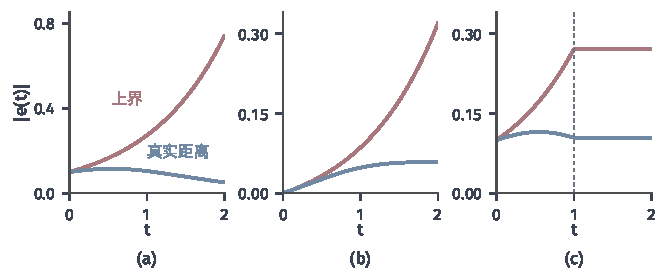
\includegraphics[width=112mm]{figures/06-differential-equations/01-ordinary-differential-equations/matplotlib/odesens-gronwall-roles/figure.pdf}
  \caption{Gronwall上界的三个成分。方程基于$\dot{x}=\sin x$，$x(0)=1$，蓝线是由数值积分得到的真实距离，红线是式~\eqref{eq:odesens-basic-estimate}的上界。(a)只有初值差$0.1$，上界$0.1\mathrm{e}^{t}$。(b)只有持续外力$r\equiv0.05$，上界$0.05(\mathrm{e}^{t}-1)$。(c)右端乘以$\beta(t)$，$\beta$在$[0,1)$上为$1$、此后为$0$，上界在$t=1$（虚线）后不再增长。}
  \label{fig:odesens-gronwall-roles}
\end{BookInlineFigure}

上界并非总是宽松的。取$\dot{x}=x$和$\dot{y}=y+0.05$，初值差$0.1$，误差方程$\dot{e}=e+0.05$可以直接解出，
\[
 e(t)=0.1\,\mathrm{e}^{t}+0.05\,(\mathrm{e}^{t}-1).
\]
这恰好是式~\eqref{eq:odesens-constant-estimate}取$L=1$、$\delta=0.05$的右端，在$t=1$时等于$0.2718+0.0859=0.3577$。可见不增加其他结构时，这个上界不能再改进。

\paragraph{去掉Lipschitz条件会怎样}
定理的结论蕴含唯一性：取$\bm{r}=\bm{0}$、$\bm{y}_0=\bm{x}_0$，上界为零。方程$\dot{x}=2\sqrt{\lvert x\rvert}$从$x(0)=0$出发有一族解，对任意$c\geq0$，
\[
 x_c(t)=\begin{cases}0,&t\leq c,\\(t-c)^2,&t>c,\end{cases}
\]
都满足方程，见图~\ref{fig:odesens-nonlipschitz-split}。比较$x_0(t)=t^2$与零解，差商是
\[
 \frac{\lvert f(t^2)-f(0)\rvert}{t^2}=\frac{2}{t},
\]
它在$t=0$附近不可积。放大系数的积分发散，式~\eqref{eq:odesens-basic-estimate}无从写起，这就是Lipschitz条件失效的具体样子。

\begin{BookInlineFigure}
  \centering
  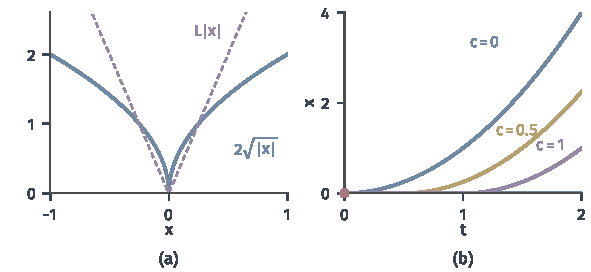
\includegraphics[width=100mm]{figures/06-differential-equations/01-ordinary-differential-equations/matplotlib/odesens-nonlipschitz-split/figure.pdf}
  \caption{没有Lipschitz条件时比较定理失效。(a)右端$2\sqrt{\lvert x\rvert}$在$x=0$处切线竖直，任何过原点的直线$L\lvert x\rvert$（紫色虚线）都压不住它。(b)同一红色初值$x(0)=0$出发的解$x_c$，$c=0,0.5,1$，蓝色水平线是零解。初值差为零，解的差却不为零。}
  \label{fig:odesens-nonlipschitz-split}
\end{BookInlineFigure}

\section{初值依赖}
\label{sec:odesens-initial}

定理~\ref{thm:odesens-basic-estimate}假设两条曲线都在$[t_0,T]$上存在，并且都留在同一个有Lipschitz常数的集合里。这对邻近初值的解并非自动成立。考虑$\dot{x}=x^2$，解是
\[
 x(t)=\frac{x_0}{1-x_0t},
\]
正初值的解在$t=1/x_0$爆炸。从$x_0=0.5$出发的解在$[0,1]$上存在，从$x_0=1.25$出发的解到$t=0.8$就没有了。

我们要回答的是：给定一条在紧区间$[t_0,T]$上存在的解，多近的初值能保证解也活到$T$，并且曲线距离可控？

\paragraph{在解的周围取一段管道}
思路是沿着已知解围一条半径为$\rho$的管道。管道是紧集，右端在里面有统一的Lipschitz常数。邻近的解只要还在管道里，Gronwall上界就成立；上界又说明它离中心线不超过$\rho/2$，碰不到管壁。图~\ref{fig:odesens-tube-continuation}中的红色虚线是一条假想的解，它要到达管壁，必须先穿过$\rho/2$的范围，这与上界矛盾。于是解出不去，也就活到了$T$。

\begin{BookInlineFigure}
  \centering
  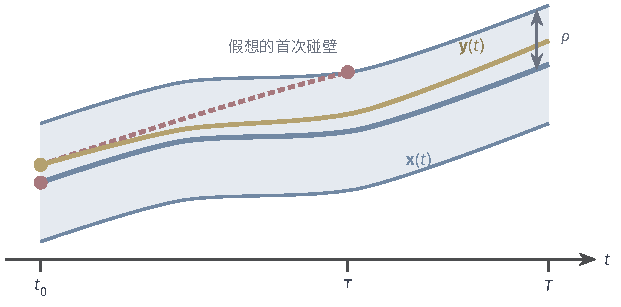
\includegraphics[width=105.2mm]{figures/06-differential-equations/01-ordinary-differential-equations/tikz/odesens-tube-continuation/figure.pdf}
  \caption{管道论证示意。浅蓝带是参考解$\bm{x}(t)$（蓝）周围半径$\rho$的管道，右端在其中有统一的Lipschitz常数。初值足够近的解$\bm{y}(t)$（黄）留在管道内。红色虚线表示假想的情形：解在$\tau$时首次碰壁，这与上界矛盾。}
  \label{fig:odesens-tube-continuation}
\end{BookInlineFigure}

图~\ref{fig:odesens-common-interval}的浅蓝带就是$\dot{x}=x^2$的管道。

\begin{BookInlineFigure}
  \centering
  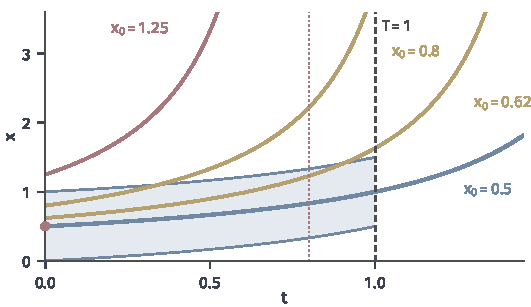
\includegraphics[width=90mm]{figures/06-differential-equations/01-ordinary-differential-equations/matplotlib/odesens-common-interval/figure.pdf}
  \caption{$\dot{x}=x^2$的邻近解。蓝色粗线从红点$x_0=0.5$出发，在$[0,1]$上存在，浅蓝带是半径$\rho=0.5$的管道。黄线$x_0=0.62$、$x_0=0.8$在$T=1$之前穿出管道，但解仍能活到$T=1$。红线$x_0=1.25$在红色点线$t=0.8$处爆炸，到不了$T=1$（灰色虚线）。}
  \label{fig:odesens-common-interval}
\end{BookInlineFigure}

证明要用第~\ref{chap:ode-existence-continuation}章的延拓结论：在局部唯一条件下，最大解若不能继续延拓，就会离开定义域内的任意紧集。也就是说，一段解如果始终留在定义域内的某个紧集里，就可以向后延伸。

\begin{theorem}[初值的局部Lipschitz依赖]
\label{thm:odesens-local-lipschitz}
设$\bm{D}\subseteq\mathbb{R}\times\mathbb{R}^{n}$是开集，$\bm{f}:\bm{D}\to\mathbb{R}^{n}$连续，且在每一点附近关于状态Lipschitz。设$\bm{x}:[t_0,T]\to\mathbb{R}^{n}$是一条解，其图像落在$\bm{D}$内。则存在$\rho>0$，使管道
\begin{equation}
 \bm{K}_\rho=\bigl\{(t,\bm{z}):t\in[t_0,T],\ \lVert\bm{z}-\bm{x}(t)\rVert_2\leq\rho\bigr\}
 \label{eq:odesens-tube}
\end{equation}
是$\bm{D}$的紧子集，$\bm{f}$在其上关于状态有统一的Lipschitz常数$L$。进一步，令$\delta=\tfrac12\rho\,\mathrm{e}^{-L(T-t_0)}$，则对每个满足$\lVert\bm{y}_0-\bm{x}_0\rVert_2\leq\delta$的$\bm{y}_0$，从$(t_0,\bm{y}_0)$出发的解在$[t_0,T]$上存在，且留在$\bm{K}_\rho$内。对两个这样的初值$\bm{y}_0$、$\bm{w}_0$，相应的解满足
\begin{equation}
 \lVert\bm{y}(t)-\bm{w}(t)\rVert_2\leq\mathrm{e}^{L(t-t_0)}\lVert\bm{y}_0-\bm{w}_0\rVert_2,\qquad t\in[t_0,T].
 \label{eq:odesens-local-lipschitz}
\end{equation}
\end{theorem}

\begin{proof}
先取管道。$\bm{x}$的图像是开集$\bm{D}$中的紧集，到$\bm{D}$的补集有正距离（$\bm{D}$是全空间时距离视为无穷）。取$\rho$小于这个距离的一半，则$\bm{K}_\rho\subset\bm{D}$，且$\bm{K}_\rho$是有界闭集，因而紧。

再说明Lipschitz常数统一。假设不然，对每个$k$有$(t_k,\bm{a}_k),(t_k,\bm{b}_k)\in\bm{K}_\rho$，使
\[
 \lVert\bm{f}(t_k,\bm{a}_k)-\bm{f}(t_k,\bm{b}_k)\rVert_2>k\lVert\bm{a}_k-\bm{b}_k\rVert_2.
\]
连续函数$\bm{f}$在紧集上有界，设界为$M$，于是$\lVert\bm{a}_k-\bm{b}_k\rVert_2<2M/k\to0$。取子列使两组点收敛到同一点$(t_\ast,\bm{z}_\ast)\in\bm{K}_\rho$。该点附近$\bm{f}$关于状态有Lipschitz常数，而$k\to\infty$与之矛盾。

现在设$\lVert\bm{y}_0-\bm{x}_0\rVert_2\leq\delta$，$\bm{y}$是最大解。令$\tau$为使$\bm{y}$在$[t_0,s]$上存在并留在$\bm{K}_\rho$内的$s\leq T$的上确界，初值在管道内部，所以$\tau>t_0$。在$[t_0,\tau)$上用定理~\ref{thm:odesens-basic-estimate}，$\bm{r}=\bm{0}$，得到
\[
 \lVert\bm{y}(t)-\bm{x}(t)\rVert_2\leq\mathrm{e}^{L(t-t_0)}\delta\leq\frac{\rho}{2}.
\]

这段解留在紧集$\bm{K}_\rho$内，由延拓结论，它可以延拓到$\tau$，且若$\tau<T$还能继续延拓到$\tau$之后。上面的不等式到$\tau$处仍成立，$\bm{y}(\tau)$离中心线不超过$\rho/2$，延拓后的一小段仍在管道内，与$\tau$的定义矛盾。所以$\tau=T$，解在闭区间$[t_0,T]$上存在且在管道内。

最后，两条解$\bm{y}$、$\bm{w}$都在$\bm{K}_\rho$内，再用一次定理~\ref{thm:odesens-basic-estimate}，就得到式~\eqref{eq:odesens-local-lipschitz}。
\end{proof}

定理中的量词值得留意。$\rho$、$L$、$\delta$都依赖给定的解和$T$，结论只在这条解附近成立，即使$\bm{f}$全局光滑也是如此。$T$越靠近这条解的爆炸时刻，管道内的$L$越大，$\delta$越小。

\begin{example}[管道的具体数字]
\label{ex:odesens-tube}
对$\dot{x}=x^2$，$x_0=1/2$，$T=1$，解$x(t)=1/(2-t)$取值在$[1/2,1]$内。取$\rho=1/2$，管道内状态在$[0,3/2]$中，$\lvert\partial_xf\rvert=2\lvert x\rvert\leq3$，所以取$L=3$。定理给出
\[
 \delta=\frac12\cdot\frac12\,\mathrm{e}^{-3}\approx0.0124.
\]

取$y_0=0.51$，它满足条件。上界给出
\[
 \lvert y(1)-x(1)\rvert\leq0.01\,\mathrm{e}^{3}\approx0.201.
\]
真实值可以直接算，
\[
 y(1)-x(1)=\frac{0.51}{0.49}-1\approx0.0408.
\]
上界偏大约五倍，因为它用整条管道上最坏的$L$。$\delta$也偏保守：实际上任何$y_0<1$的解都能活到$T=1$。定理的作用是不解方程也给出保证。
\end{example}

\paragraph{连续依赖与Lipschitz依赖}
定理~\ref{thm:odesens-local-lipschitz}的结论是\term{Lipschitz依赖}（Lipschitz dependence）：解的差不超过初值差的常数倍。更弱的要求是\term{连续依赖}（continuous dependence）：对任意$\varepsilon>0$，存在$\delta>0$，初值差小于$\delta$时，$[t_0,T]$上的解差小于$\varepsilon$。两者在依赖的“速度”上不同，所需条件也不同，见表~\ref{tab:odesens-dependence}。

\begin{BookInlineTable}
  \centering
  \caption{初值依赖的层次。结论都是给定解附近、紧时间段上的局部结论。}
  \label{tab:odesens-dependence}
  \begin{tabular}{p{28mm}p{32mm}p{38mm}}
    \toprule
    右端条件 & 依赖性质 & 例子 \\
    \midrule
    连续，解不唯一 & 流映射没有定义 & $\dot{x}=2\sqrt{\lvert x\rvert}$ \\
    连续，解唯一 & 连续依赖 & $\dot{x}=-x\ln\lvert x\rvert$ \\
    局部Lipschitz & Lipschitz依赖 & $\dot{x}=\lvert x\rvert$ \\
    连续可微 & 可微依赖（第~\ref{sec:odesens-variational}节） & $\dot{x}=x(1-x)$ \\
    \bottomrule
  \end{tabular}
\end{BookInlineTable}

第二行的结论是：右端仅连续时，只要过每个邻近初值的解都唯一，连续依赖仍然成立。证明需要用到等度连续曲线族的紧性（Arzelà--Ascoli定理）并配合延拓，篇幅较长，读者可查阅常微分方程教材。其机制是：邻近初值的解构成一族等度连续的曲线，任何收敛子列的极限都是初值问题的解，唯一性迫使极限只能是原来那条解。这个论证没有给出收敛的速度。

没有速度保证的情形确实存在。方程$\dot{x}=-x\ln\lvert x\rvert$（约定在$x=0$处右端为$0$）在$x=0$处斜率趋于无穷，右端不Lipschitz，但解仍唯一。对$0<x_0<1$，令$v=\ln x$，方程化为$\dot{v}=-v$，于是
\[
 x(t)=x_0^{\mathrm{e}^{-t}}.
\]
若有解从$0$离开，变量$v$要在有限时间内从$-\infty$变为有限值，而$\dot{v}=-v$的解不会在有限时间内从无穷回来，所以$x\equiv0$是从$0$出发的唯一解。

取$t=\ln2$，解的映射是$x_0\mapsto\sqrt{x_0}$。$x_0=10^{-4}$时解是$10^{-2}$，初值差被放大$100$倍；$x_0=10^{-8}$时放大$10^{4}$倍。比值$\sqrt{x_0}/x_0$没有上界，所以不存在Lipschitz常数。依赖仍然连续，因为$x_0\to0$时$\sqrt{x_0}\to0$，见图~\ref{fig:odesens-holder-flow}。

\begin{BookInlineFigure}
  \centering
  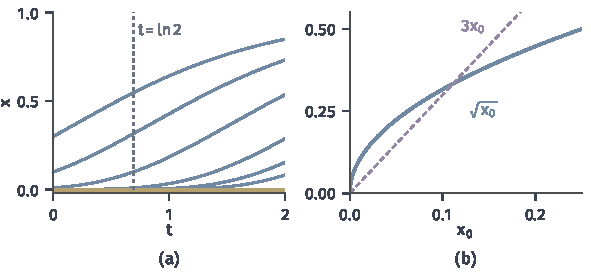
\includegraphics[width=100mm]{figures/06-differential-equations/01-ordinary-differential-equations/matplotlib/odesens-holder-flow/figure.pdf}
  \caption{连续依赖但不Lipschitz。(a)$\dot{x}=-x\ln x$从$x_0=10^{-8},10^{-6},10^{-4},10^{-2},0.1,0.3$出发的解（蓝）和零解（黄）。极小的初值很快被拉开。(b)$t=\ln2$时的解映射$\sqrt{x_0}$，在$x_0=0$处切线竖直，任何直线（紫色虚线）在原点附近都压不住它。}
  \label{fig:odesens-holder-flow}
\end{BookInlineFigure}

\paragraph{有限时间上界不是长期稳定判据}
式~\eqref{eq:odesens-local-lipschitz}的常数$\mathrm{e}^{L(T-t_0)}$随$T$指数增长。它只是有限时间的上界，不能用来判断解在长时间下靠拢还是分离。图~\ref{fig:odesens-bound-vs-true}用$L=1$的三个方程作对比，初值差都是$0.01$。

\begin{BookInlineFigure}
  \centering
  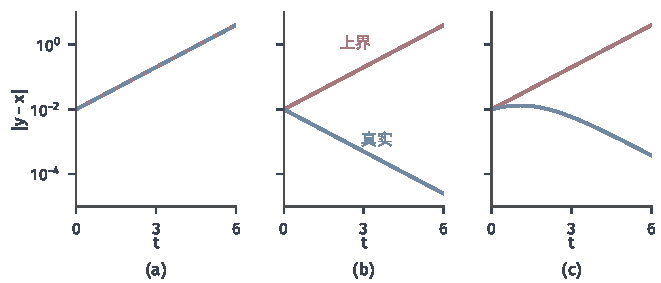
\includegraphics[width=112mm]{figures/06-differential-equations/01-ordinary-differential-equations/matplotlib/odesens-bound-vs-true/figure.pdf}
  \caption{同一个上界$0.01\,\mathrm{e}^{t}$（红）与三种真实距离（蓝，对数纵轴）。(a)$\dot{x}=x$，上界就是真实距离。(b)$\dot{x}=-x$，真实距离按$\mathrm{e}^{-t}$衰减。(c)$\dot{x}=x(1-x)$，$x_0=0.25$，距离先增后减。}
  \label{fig:odesens-bound-vs-true}
\end{BookInlineFigure}

三种情形的$L$相同，长期行为却完全不同，因为$L$只记录了$\lvert\partial_xf\rvert$的大小，丢掉了符号。反过来，$\mathrm{e}^{L(T-t_0)}$在任何固定的$T$上都有限，这也不说明解在$T\to\infty$时保持靠近。长期行为需要吸引性、不变集等额外结构，可参考\BookChapterRef{chap:dynamical-systems-long-term}{卷九第1章“动力系统与轨迹的长期行为”}。

\paragraph{保留符号信息}
能否在估计里留下符号？引理~\ref{lem:odesens-gronwall}的积分形式要求$\beta\geq0$，但如果直接对距离的平方求导，放大率可以取负。为此把Lipschitz条件换成只约束相互靠近方向的条件，称为\term{单侧Lipschitz条件}（one-sided Lipschitz condition）。

\begin{lemma}[单侧Lipschitz估计]
\label{lem:odesens-one-sided}
设$\bm{x},\bm{y}:[t_0,T]\to\bm{K}$绝对连续，几乎处处满足$\dot{\bm{x}}=\bm{f}(t,\bm{x})$、$\dot{\bm{y}}=\bm{f}(t,\bm{y})$。设实值函数$\mu$可积（可以取负值），且对几乎每个$t$及所有$\bm{a},\bm{b}\in\bm{K}$，
\begin{equation}
 \bigl\langle\bm{f}(t,\bm{a})-\bm{f}(t,\bm{b}),\,\bm{a}-\bm{b}\bigr\rangle\leq\mu(t)\lVert\bm{a}-\bm{b}\rVert_2^2.
 \label{eq:odesens-one-sided}
\end{equation}
则对每个$t\in[t_0,T]$，
\begin{equation}
 \lVert\bm{y}(t)-\bm{x}(t)\rVert_2\leq\lVert\bm{y}_0-\bm{x}_0\rVert_2\,\exp\int_{t_0}^{t}\mu(s)\,\mathrm{d}s.
 \label{eq:odesens-one-sided-bound}
\end{equation}
\end{lemma}

\begin{proof}
令$v=\lVert\bm{y}-\bm{x}\rVert_2^2$，$v$绝对连续。由式~\eqref{eq:odesens-one-sided}，几乎处处有
\[
 \dot{v}=2\bigl\langle\bm{f}(t,\bm{y})-\bm{f}(t,\bm{x}),\,\bm{y}-\bm{x}\bigr\rangle\leq2\mu v.
\]
记$M(t)=\int_{t_0}^{t}\mu$，乘以积分因子后得到
\[
 \frac{\mathrm{d}}{\mathrm{d}t}\bigl(\mathrm{e}^{-2M}v\bigr)\leq0.
\]
所以$v(t)\leq\mathrm{e}^{2M(t)}v(t_0)$，开方即得结论。
\end{proof}

对$\dot{x}=-x$，条件式成立且$\mu=-1$，式~\eqref{eq:odesens-one-sided-bound}恰好是真实的$\mathrm{e}^{-t}$衰减。对$\dot{x}=-x^3$，
\[
 (a-b)(-a^3+b^3)=-(a-b)^2(a^2+ab+b^2)\leq0,
\]
可取$\mu=0$，而这个右端在$\mathbb{R}$上没有全局Lipschitz常数。这样的方程上任意两条解的距离不增，这比用$L$的上界强得多。该结论同样只陈述了给定时间段上的比较，并不涉及平衡点的吸引。

\section{参数与输入扰动}
\label{sec:odesens-parameter-input}

初值只是数据的一部分。方程里的系数是估计出来的，外部输入有噪声，方程本身也只是对真实规律的近似。这些改变看上去性质各异，其实都改变了同一件事：曲线每一时刻的变化率。它们都可以写成积分方程中的残差，于是定理~\ref{thm:odesens-basic-estimate}一次解决全部情形。

\paragraph{统一成积分方程中的扰动}
设$\bm{x}$解$\dot{\bm{x}}=\bm{f}(t,\bm{x})$，$\bm{y}$解被改变的方程$\dot{\bm{y}}=\tilde{\bm{f}}(t,\bm{y})$。把$\bm{y}$的方程改写成
\[
 \dot{\bm{y}}=\bm{f}(t,\bm{y})+\bm{r}(t),\qquad
 \bm{r}(t)=\tilde{\bm{f}}(t,\bm{y}(t))-\bm{f}(t,\bm{y}(t)).
\]
这里$\bm{r}$沿着曲线$\bm{y}$取值，是一个只依赖时间的函数。图~\ref{fig:odesens-perturbation-sources}列出了各种改变的去向。

\begin{BookInlineFigure}
  \centering
  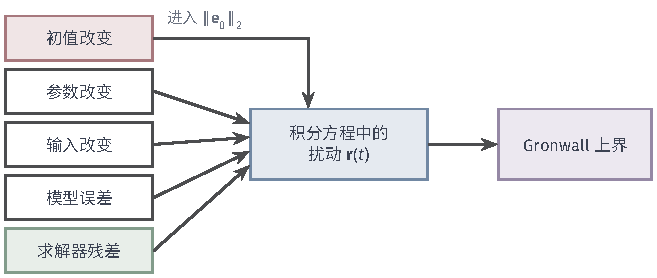
\includegraphics[width=111.2mm]{figures/06-differential-equations/01-ordinary-differential-equations/tikz/odesens-perturbation-sources/figure.pdf}
  \caption{各类改变进入同一个估计的路径。初值改变进入起点的差，参数、输入、模型与数值计算的改变都写成随时间变化的残差$\bm{r}(t)$，再由式~\eqref{eq:odesens-basic-estimate}转成曲线距离的上界。}
  \label{fig:odesens-perturbation-sources}
\end{BookInlineFigure}

\begin{theorem}[右端扰动下的比较]
\label{thm:odesens-perturbation}
设$\bm{x},\bm{y}:[t_0,T]\to\bm{K}$绝对连续，分别几乎处处满足$\dot{\bm{x}}=\bm{f}(t,\bm{x})$、$\dot{\bm{y}}=\tilde{\bm{f}}(t,\bm{y})$。设$\bm{f}$在$\bm{K}$上满足式~\eqref{eq:odesens-lipschitz}，$L$可积，且残差
\begin{equation}
 \varepsilon(t)=\bigl\lVert\tilde{\bm{f}}(t,\bm{y}(t))-\bm{f}(t,\bm{y}(t))\bigr\rVert_2
 \label{eq:odesens-residual}
\end{equation}
可积。记$\Lambda(t)=\int_{t_0}^{t}L$。则
\begin{equation}
 \lVert\bm{y}(t)-\bm{x}(t)\rVert_2\leq\mathrm{e}^{\Lambda(t)}\lVert\bm{y}_0-\bm{x}_0\rVert_2+\int_{t_0}^{t}\mathrm{e}^{\Lambda(t)-\Lambda(s)}\varepsilon(s)\,\mathrm{d}s.
 \label{eq:odesens-perturbation-bound}
\end{equation}
\end{theorem}

\begin{proof}
取定理前定义的残差$\bm{r}$，则$\lVert\bm{r}\rVert_2=\varepsilon$，$\bm{y}$满足定理~\ref{thm:odesens-basic-estimate}中带残差的方程。代入式~\eqref{eq:odesens-basic-estimate}即得结论。
\end{proof}

定理只要求$\bm{f}$有Lipschitz常数，对$\tilde{\bm{f}}$没有要求，它甚至可以不连续。这在比较真实系统与简化模型时有用：真实规律$\tilde{\bm{f}}$往往未知也不光滑，只要它的轨迹$\bm{y}$存在，并且能估计模型在这条轨迹上的误差$\varepsilon$。定理的$\bm{y}$仍须事先知道留在$\bm{K}$内；$\bm{f}$与$\tilde{\bm{f}}$足够接近时，第~\ref{sec:odesens-initial}节的管道论证可以保证这一点。

\paragraph{参数改变}
设右端依赖参数$\bm{\theta}$，且关于参数满足
\[
 \lVert\bm{f}(t,\bm{a},\tilde{\bm{\theta}})-\bm{f}(t,\bm{a},\bm{\theta})\rVert_2\leq\ell(t)\lVert\tilde{\bm{\theta}}-\bm{\theta}\rVert_2,
\]
其中$\ell$可积。此时残差不超过$\ell(s)$乘以参数差的范数，初值相同时，式~\eqref{eq:odesens-perturbation-bound}化为
\begin{equation}
 \lVert\bm{y}(t)-\bm{x}(t)\rVert_2\leq\lVert\tilde{\bm{\theta}}-\bm{\theta}\rVert_2\int_{t_0}^{t}\mathrm{e}^{\Lambda(t)-\Lambda(s)}\ell(s)\,\mathrm{d}s.
 \label{eq:odesens-parameter-bound}
\end{equation}
所以解在紧时间段上Lipschitz依赖参数，前提与初值情形相同。

\begin{example}[增长率改变$20\%$]
\label{ex:odesens-parameter-bound}
考虑$\dot{x}=\theta x(1-x)$，$x_0=1/4$，比较$\theta=1$与$\tilde{\theta}=1.2$在$T=\ln3$时的值。解都留在$\bm{K}=[0,1]$内，$\theta=1$的右端关于$x$的导数是$1-2x$，取$L=1$。残差是
\[
 r(s)=0.2\,y(s)\bigl(1-y(s)\bigr),\qquad \lvert r(s)\rvert\leq0.05.
\]

用$\lvert r\rvert\leq0.05$的粗略界，由式~\eqref{eq:odesens-constant-estimate}得到
\[
 \lvert y(T)-x(T)\rvert\leq0.05\,(\mathrm{e}^{T}-1)=0.1.
\]
若把残差沿$y$的实际值代入式~\eqref{eq:odesens-perturbation-bound}，数值积分得到上界$0.0901$。真实差是$y(T)-x(T)=0.5547-0.5=0.0547$。
\end{example}

图~\ref{fig:odesens-parameter-bound}显示了$[0,3]$上的情况。上界在$t$较大时远离真实差，原因和图~\ref{fig:odesens-bound-vs-true}(c)相同：$L=1$对应$x$靠近$0$时的增长，而$x$靠近$1$时真实的放大率是负的。

\begin{BookInlineFigure}
  \centering
  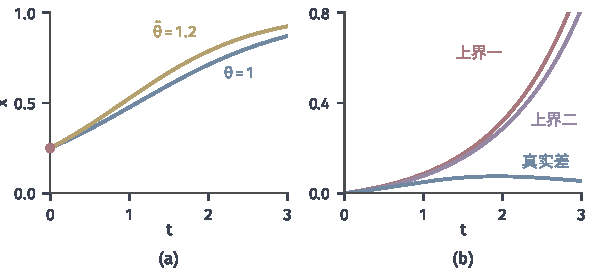
\includegraphics[width=100mm]{figures/06-differential-equations/01-ordinary-differential-equations/matplotlib/odesens-parameter-bound/figure.pdf}
  \caption{参数改变对$\dot{x}=\theta x(1-x)$的影响，$x_0=1/4$。(a)$\theta=1$（蓝）与$\tilde\theta=1.2$（黄）的解。(b)两解的真实差（蓝）、用$\lvert r\rvert\leq0.05$的上界一（红）和用残差实际值的上界二（紫）。}
  \label{fig:odesens-parameter-bound}
\end{BookInlineFigure}

\paragraph{输入改变}
设方程是$\dot{\bm{x}}=\bm{f}(t,\bm{x},\bm{g}(t))$，$\bm{g}$是可测的外部输入。应该用什么范数衡量输入的差？答案取决于右端怎样依赖输入，我们看三种情形。

设右端关于输入值Lipschitz，
\[
 \lVert\bm{f}(t,\bm{a},\tilde{\bm{g}})-\bm{f}(t,\bm{a},\bm{g})\rVert_2\leq\ell(t)\lVert\tilde{\bm{g}}-\bm{g}\rVert_2.
\]
线性输入$\bm{f}=\bm{a}(t,\bm{x})+\bm{B}(t)\bm{g}$就是这样，$\ell(t)=\lVert\bm{B}(t)\rVert_2$。此时$\varepsilon$由输入差的加权积分控制，
\begin{equation}
 \int_{t_0}^{T}\varepsilon(s)\,\mathrm{d}s\leq\int_{t_0}^{T}\ell(s)\,\lVert\tilde{\bm{g}}(s)-\bm{g}(s)\rVert_2\,\mathrm{d}s.
 \label{eq:odesens-input-l1}
\end{equation}
这里合适的度量是积分范数，也就是$L^1$范数，瞬时的巨大偏差只要持续够短，影响就小。图~\ref{fig:odesens-input-norms}(a)中方程为$\dot{x}=-x+g$，偏差是$[1,1.02)$上高度$5$的脉冲，积分等于$0.1$。解的差不超过$0.1$，实际在$t=1.02$时达到$5(1-\mathrm{e}^{-0.02})\approx0.099$，然后衰减，到$t=2$时约为$0.037$。

\begin{BookInlineFigure}
  \centering
  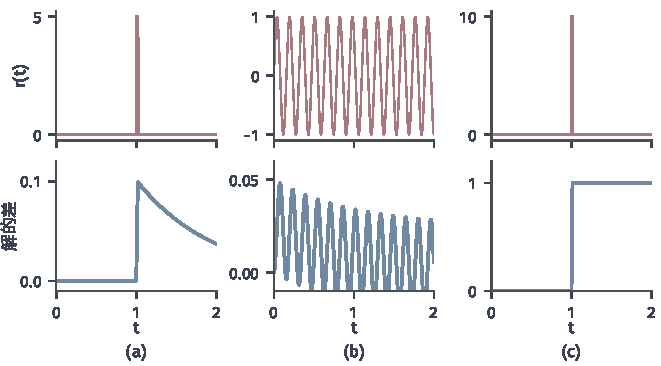
\includegraphics[width=112mm]{figures/06-differential-equations/01-ordinary-differential-equations/matplotlib/odesens-input-norms/figure.pdf}
  \caption{输入差的大小与解的差。上行是输入偏差$r(t)$，下行是解的差。(a)$\dot{x}=-x+g$，脉冲高$5$、宽$0.02$，积分$0.1$，解的差不超过$0.1$。(b)$\dot{x}=-x+g$，偏差$\sin40t$，积分范数约$1.27$，解的差却不超过$0.05$。(c)$\dot{x}=g^2$，脉冲高$10$、宽$0.01$，积分同为$0.1$，解的差却达到$1$。}
  \label{fig:odesens-input-norms}
\end{BookInlineFigure}

式~\eqref{eq:odesens-input-l1}是充分条件，不是必要条件。图~\ref{fig:odesens-input-norms}(b)的偏差$\sin40t$在$[0,2]$上的积分范数约为$1.27$，解的差却不超过$0.05$。原因是正负部分抵消，在加性输入下真正起作用的是偏差的累积$\int_{t_0}^{t}\bm{r}(s)\,\mathrm{d}s$，这里它不超过$2/40=0.05$。

非线性依赖就不同了。方程$\dot{x}=g^2$的残差是$\tilde{g}^2-g^2$，关于$g$的增长率随$\lvert g\rvert$变大。取$g\equiv0$，$\tilde{g}$是$[1,1+w)$上高度$A$的脉冲，
\[
 \int_0^2\lvert\tilde{g}-g\rvert\,\mathrm{d}t=Aw,\qquad y(2)-x(2)=A^2w.
\]
令$A=10$、$w=0.01$，输入差的积分只有$0.1$，解的差却是$1$，见图~\ref{fig:odesens-input-norms}(c)。让$A\to\infty$并保持$A^2w=1$，积分范数趋于零而解差不变。所以这里$L^1$小不足以保证解差小。

补救有两条路。若所有输入的值都限制在$\lVert\bm{g}\rVert_2\leq M$内，右端在这个范围内关于$\bm{g}$有常数$\ell=2M$，式~\eqref{eq:odesens-input-l1}恢复成立，$M$进入常数；上例$M=10$，$\ell\cdot Aw=20\times0.1=2$，确实不小于真实的$1$。另一条路是用更强的范数：一致范数$\sup_t\lVert\tilde{\bm{g}}-\bm{g}\rVert_2$小，就排除了高而窄的脉冲，只是它对孤立的短暂偏差过于敏感。

\paragraph{可测输入的条件}
上面的估计都只用到残差可积，没有用到输入的连续性。分段切换的输入、一般可测的输入都在其中，此时解是绝对连续函数，方程几乎处处成立。沿用第~\ref{chap:ode-existence-continuation}章的Carathéodory条件，右端沿解的复合是可测且局部可积的，式~\eqref{eq:odesens-residual}的$\varepsilon$因而有意义。但要得到定理~\ref{thm:odesens-basic-estimate}的结论，仍需要对时间可积的状态Lipschitz系数$L(t)$，这不是可测性能推出的。

\paragraph{方程的敏感性与求解器误差}
数值解也可以放进这个框架，这样能把两种常被混淆的误差分开。下面的计算只用定理的结构，数值方法本身放在第~\ref{chap:ode-numerical-methods}章。设网格$t_k=t_0+kh$，从$\bm{x}^{(0)}=\bm{x}_0$出发按
\[
 \bm{x}^{(k+1)}=\bm{x}^{(k)}+h\,\bm{f}(t_k,\bm{x}^{(k)})
\]
前进，把各点连成折线$\bm{y}(t)$。折线绝对连续，它的残差是$\bm{r}(s)=\dot{\bm{y}}(s)-\bm{f}(s,\bm{y}(s))$。

代入式~\eqref{eq:odesens-basic-estimate}，全局误差的上界是残差与放大因子乘积的积分。残差由求解器决定，步长越小残差越小。放大因子$\mathrm{e}^{\Lambda(t)-\Lambda(s)}$由方程决定，与求解器无关。前者是求解器的误差来源，后者是问题本身的敏感性。

\begin{example}[同一求解器，两个方程]
\label{ex:odesens-problem-solver}
取$\dot{x}=ax$，$x_0=1$，$h=1/4$，$T=1$，$a=\pm1$。在$[t_k,t_{k+1})$上，折线是$y(s)=x^{(k)}(1+a(s-t_k))$，于是
\[
 r(s)=\dot{y}-ay=-a^2x^{(k)}(s-t_k).
\]
方程线性，误差方程$\dot{e}=ae+r$可以精确求解，初值差为零时
\[
 y(1)-\mathrm{e}^{a}=\int_0^1\mathrm{e}^{a(1-s)}r(s)\,\mathrm{d}s.
\]

$a=1$时，$x^{(k)}$依次是$1,\,1.25,\,1.5625,\,1.9531,\,2.4414$；$a=-1$时依次是$1,\,0.75,\,0.5625,\,0.4219,\,0.3164$。逐段积分，得到
\[
 a=1:\ y(1)-\mathrm{e}=-0.2769,\qquad a=-1:\ y(1)-\mathrm{e}^{-1}=-0.0515.
\]
\end{example}

图~\ref{fig:odesens-problem-vs-solver}把三个量画在一起。两个方程的残差都是锯齿形，大小同为$h$的量级。权重却相反：$a=1$时早期残差被放大$\mathrm{e}^{1-s}>1$倍，$a=-1$时被缩小。误差相差五倍多，主要来自方程，而不是求解器。

\begin{BookInlineFigure}
  \centering
  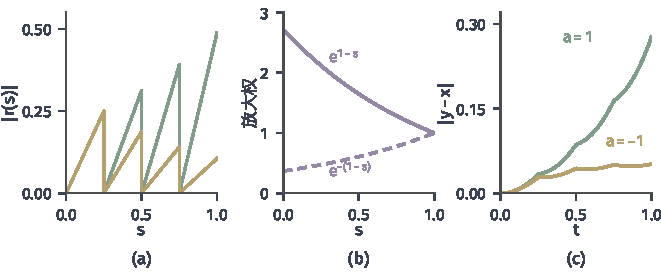
\includegraphics[width=112mm]{figures/06-differential-equations/01-ordinary-differential-equations/matplotlib/odesens-problem-vs-solver/figure.pdf}
  \caption{同一求解器在$\dot{x}=ax$上的表现，$h=1/4$，绿线$a=1$，黄线$a=-1$。(a)Euler折线的残差$\lvert r(s)\rvert$，由求解器决定。(b)放大权$\mathrm{e}^{a(1-s)}$，由方程决定（紫实线$a=1$，紫虚线$a=-1$）。(c)累积后的误差。}
  \label{fig:odesens-problem-vs-solver}
\end{BookInlineFigure}

因此，问题敏感时，再精细的求解器也只能把残差压小，放大因子还在；问题不敏感时，粗糙的残差也不至于造成大的全局误差。把解算准需要两者配合，这两者不可相互替代。


\section{变分方程}
\label{sec:odesens-variational}

Gronwall估计只回答“差多少”，不回答“往哪边差”，得到的常数也往往偏大。若解关于数据可微，初值沿某方向变一点时，解的变化就可以用一个线性方程精确算到一阶。这需要先弄清楚解什么时候可微。

\paragraph{连续依赖不能推出可微依赖}
方程$\dot{x}=\lvert x\rvert$的右端全局Lipschitz，$L=1$，解对初值Lipschitz依赖。可是$x_0>0$时解是$x_0\mathrm{e}^{t}$，$x_0<0$时解是$x_0\mathrm{e}^{-t}$，所以
\[
 \varphi_1(x_0)=\begin{cases}\mathrm{e}\,x_0,&x_0\geq0,\\x_0/\mathrm{e},&x_0<0.\end{cases}
\]
$\varphi_1$在$x_0=0$处左导数为$1/\mathrm{e}$，右导数为$\mathrm{e}$，不可微，见图~\ref{fig:odesens-kink}。Lipschitz依赖只限制了差商的大小，并不保证差商有极限。要谈导数，右端本身要可微。

\begin{BookInlineFigure}
  \centering
  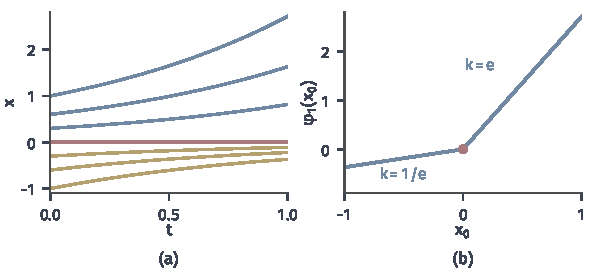
\includegraphics[width=100mm]{figures/06-differential-equations/01-ordinary-differential-equations/matplotlib/odesens-kink/figure.pdf}
  \caption{Lipschitz依赖而不可微。(a)$\dot{x}=\lvert x\rvert$的解：正初值（蓝）按$\mathrm{e}^{t}$增长，负初值（黄）按$\mathrm{e}^{-t}$衰减，红线是零解。(b)$t=1$时的解映射，在红点$x_0=0$处有折点，左右斜率分别为$1/\mathrm{e}$与$\mathrm{e}$。}
  \label{fig:odesens-kink}
\end{BookInlineFigure}

\paragraph{形式推导}
先假设可以求导，看导数应当满足什么方程。设$\bm{x}(t;\bm{x}_0,\bm{\theta})$解
\[
 \dot{\bm{x}}=\bm{f}(t,\bm{x},\bm{\theta}),\qquad \bm{x}(t_0)=\bm{x}_0,
\]
参考解记为$\bm{x}(t)$。沿方向$(\bm{v},\bm{w})$扰动，考虑$\bm{x}(t;\bm{x}_0+\varepsilon\bm{v},\bm{\theta}+\varepsilon\bm{w})$。把积分方程对$\varepsilon$在$0$处求导，记$\bm{z}(t)$为解的方向导数，由链式法则，
\[
 \bm{z}(t)=\bm{v}+\int_{t_0}^{t}\bigl[\bm{A}(s)\bm{z}(s)+\bm{B}(s)\bm{w}\bigr]\,\mathrm{d}s,
\]
其中两个系数沿参考解取值：
\begin{equation}
 \bm{A}(t)=\partial_{\bm{x}}\bm{f}\bigl(t,\bm{x}(t),\bm{\theta}\bigr),\qquad
 \bm{B}(t)=\partial_{\bm{\theta}}\bm{f}\bigl(t,\bm{x}(t),\bm{\theta}\bigr).
 \label{eq:odesens-coefficients}
\end{equation}
这就是
\begin{equation}
 \dot{\bm{z}}=\bm{A}(t)\bm{z}+\bm{B}(t)\bm{w},\qquad \bm{z}(t_0)=\bm{v},
 \label{eq:odesens-variational}
\end{equation}
称为沿参考解的\term{变分方程}（variational equation）。

原方程是非线性的，变分方程却是线性的，系数是沿已知轨迹取值的时变矩阵，第~\ref{chap:linear-differential-systems}章的工具全部可用。上面的推导把求导和积分交换了，也默认了导数存在，下面的定理补上这两点。

\begin{theorem}[解的可微依赖]
\label{thm:odesens-differentiable}
设$\bm{U}\subseteq\mathbb{R}^{n}$、$\bm{\Theta}\subseteq\mathbb{R}^{p}$是开集，取值于$\mathbb{R}^{n}$的右端$\bm{f}$定义在$[t_0,T]\times\bm{U}\times\bm{\Theta}$上，满足：对固定的$(\bm{a},\bm{\theta})$关于$t$可测；对几乎每个$t$，关于$(\bm{a},\bm{\theta})$连续可微。设$\bm{x}:[t_0,T]\to\bm{U}$是参数$\bm{\theta}$、初值$\bm{x}_0$的绝对连续解，并设存在$\rho>0$与可积函数$m\geq0$，使闭管道$\lVert\bm{a}-\bm{x}(t)\rVert_2\leq\rho$落在$\bm{U}$内，闭球$\lVert\bm{\vartheta}-\bm{\theta}\rVert_2\leq\rho$落在$\bm{\Theta}$内，且在其上对几乎每个$t$有
\begin{equation}
 \lVert\partial_{\bm{x}}\bm{f}(t,\bm{a},\bm{\vartheta})\rVert_2\leq m(t),\qquad
 \lVert\partial_{\bm{\theta}}\bm{f}(t,\bm{a},\bm{\vartheta})\rVert_2\leq m(t).
 \label{eq:odesens-derivative-bound}
\end{equation}
则存在$\delta>0$，当$\lVert\bm{v}\rVert_2+\lVert\bm{w}\rVert_2<\delta$时，初值$\bm{x}_0+\bm{v}$、参数$\bm{\theta}+\bm{w}$的解$\bm{y}$在$[t_0,T]$上存在且唯一，并且
\begin{equation}
 \sup_{t\in[t_0,T]}\bigl\lVert\bm{y}(t)-\bm{x}(t)-\bm{z}(t)\bigr\rVert_2=o\bigl(\lVert\bm{v}\rVert_2+\lVert\bm{w}\rVert_2\bigr),
 \label{eq:odesens-differentiable}
\end{equation}
其中$\bm{z}$是变分方程~\eqref{eq:odesens-variational}的解。
\end{theorem}

\begin{proof}
记扰动的大小为
\[
 \lVert\bm{\eta}\rVert=\lVert\bm{v}\rVert_2+\lVert\bm{w}\rVert_2,
\]
并记$M=\int_{t_0}^{T}m$。

\emph{第一步，解的存在与线性控制。}由式~\eqref{eq:odesens-derivative-bound}和中值不等式，右端在管道内关于状态有Lipschitz系数$m(t)$，关于参数有系数$m(t)$。按定理~\ref{thm:odesens-local-lipschitz}的管道论证，把常数$L$换成可积系数$m(t)$，并使用第~\ref{chap:ode-existence-continuation}章Carathéodory情形的延拓结论，只要$\delta$足够小，$\bm{y}$就在$[t_0,T]$上存在并留在管道内。由式~\eqref{eq:odesens-perturbation-bound}，取残差$\varepsilon\leq m\lVert\bm{w}\rVert_2$，
\[
 \lVert\bm{y}(t)-\bm{x}(t)\rVert_2\leq\mathrm{e}^{M}\lVert\bm{v}\rVert_2+M\mathrm{e}^{M}\lVert\bm{w}\rVert_2\leq C\lVert\bm{\eta}\rVert,
\]
其中$C=(1+M)\mathrm{e}^{M}$。

\emph{第二步，写出余项的方程。}记$\bm{\Delta}=\bm{y}-\bm{x}$，$\bm{R}=\bm{\Delta}-\bm{z}$，则$\bm{R}(t_0)=\bm{0}$。对几乎每个固定的$t$，沿线段$\sigma\mapsto(\bm{x}+\sigma\bm{\Delta},\bm{\theta}+\sigma\bm{w})$用微积分基本定理，
\[
 \bm{f}(t,\bm{y},\bm{\theta}+\bm{w})-\bm{f}(t,\bm{x},\bm{\theta})
 =\int_0^1\bigl[\partial_{\bm{x}}\bm{f}^{\sigma}\,\bm{\Delta}+\partial_{\bm{\theta}}\bm{f}^{\sigma}\,\bm{w}\bigr]\,\mathrm{d}\sigma,
\]
$\partial\bm{f}^{\sigma}$表示在线段上$\sigma$处取值。减去$\bm{A}\bm{z}+\bm{B}\bm{w}$，得到
\[
 \dot{\bm{R}}=\bm{A}\bm{R}+\bm{E},\qquad
 \bm{E}(t)=\int_0^1\bigl[(\partial_{\bm{x}}\bm{f}^{\sigma}-\bm{A})\bm{\Delta}+(\partial_{\bm{\theta}}\bm{f}^{\sigma}-\bm{B})\bm{w}\bigr]\,\mathrm{d}\sigma.
\]

\emph{第三步，估计$\bm{E}$。}定义
\[
 \omega_{\bm{\eta}}(t)=\sup\bigl(\lVert\partial_{\bm{x}}\bm{f}(t,\bm{a},\bm{\vartheta})-\bm{A}(t)\rVert_2+\lVert\partial_{\bm{\theta}}\bm{f}(t,\bm{a},\bm{\vartheta})-\bm{B}(t)\rVert_2\bigr),
\]
上确界取遍满足下式的$(\bm{a},\bm{\vartheta})$：
\[
 \lVert\bm{a}-\bm{x}(t)\rVert_2\leq C\lVert\bm{\eta}\rVert,\qquad\lVert\bm{\vartheta}-\bm{\theta}\rVert_2\leq\lVert\bm{\eta}\rVert.
\]
被取上确界的量关于$(\bm{a},\bm{\vartheta})$连续，上确界可以改取可数稠密子集，所以$\omega_{\bm{\eta}}$可测。由第一步，
\[
 \lVert\bm{E}(t)\rVert_2\leq\omega_{\bm{\eta}}(t)\bigl(\lVert\bm{\Delta}(t)\rVert_2+\lVert\bm{w}\rVert_2\bigr)\leq(C+1)\lVert\bm{\eta}\rVert\,\omega_{\bm{\eta}}(t).
\]

\emph{第四步，取极限。}对$\dot{\bm{R}}=\bm{A}\bm{R}+\bm{E}$取积分形式与范数，得到
\[
 \lVert\bm{R}(t)\rVert_2\leq\int_{t_0}^{t}\bigl(m\lVert\bm{R}\rVert_2+\lVert\bm{E}\rVert_2\bigr)\,\mathrm{d}s.
\]
由引理~\ref{lem:odesens-gronwall}，
\[
 \sup_{t}\lVert\bm{R}(t)\rVert_2\leq\mathrm{e}^{M}(C+1)\lVert\bm{\eta}\rVert\int_{t_0}^{T}\omega_{\bm{\eta}}(s)\,\mathrm{d}s.
\]
当$\lVert\bm{\eta}\rVert\to0$时，由导数对$(\bm{a},\bm{\vartheta})$的连续性，$\omega_{\bm{\eta}}\to0$几乎处处成立；又$\omega_{\bm{\eta}}\leq4m$可积。控制收敛定理给出$\int\omega_{\bm{\eta}}\to0$，这就是式~\eqref{eq:odesens-differentiable}。
\end{proof}

定理的条件各有分工。对状态和参数连续可微，保证了第三步的$\omega_{\bm{\eta}}\to0$，把它换成Lipschitz就会出现$\lvert x\rvert$那样的折点。统一的可积上界$m$既给出第一步的管道，也提供控制收敛定理所需的控制函数。对时间只要求可测，所以$\bm{A}$、$\bm{B}$可以在输入切换的时刻跳变，变分方程几乎处处成立。

对$\bm{v},\bm{w}$而言，$\bm{z}$是线性的，所以式~\eqref{eq:odesens-differentiable}说的正是解映射在该点Fréchet可微。把参考点也变动，$\bm{A}$、$\bm{B}$按$L^1$连续变化（同样由控制收敛定理），线性方程的解也随之连续变化，因此解映射是连续可微的。这里所有结论只针对给定解的管道内。

\paragraph{一阶预测与余项}
变分方程给出一阶预测$\bm{y}\approx\bm{x}+\bm{z}$。余项$o(\cdot)$说明小扰动下预测越来越准，但没有说多小才算小。若导数本身Lipschitz，余项可以写出来。

\begin{theorem}[一阶预测的余项]
\label{thm:odesens-remainder}
在定理~\ref{thm:odesens-differentiable}的设定中，只改变初值（$\bm{w}=\bm{0}$），设$\bm{y}$与$\bm{x}$之间的线段留在管道内，$\lVert\partial_{\bm{x}}\bm{f}\rVert_2\leq L$，且$\partial_{\bm{x}}\bm{f}$关于状态有Lipschitz常数$M_2$，$L>0$。则
\begin{equation}
 \lVert\bm{y}(t)-\bm{x}(t)-\bm{z}(t)\rVert_2\leq\frac{M_2}{2}\,\lVert\bm{v}\rVert_2^2\,\frac{\mathrm{e}^{L(t-t_0)}\bigl(\mathrm{e}^{L(t-t_0)}-1\bigr)}{L}.
 \label{eq:odesens-remainder}
\end{equation}
\end{theorem}

\begin{proof}
沿用上一定理第二步的记号，$\bm{w}=\bm{0}$。线段上$\sigma$处的$\partial_{\bm{x}}\bm{f}$与$\bm{A}$相差不超过$M_2\sigma\lVert\bm{\Delta}\rVert_2$，所以
\[
 \lVert\bm{E}(s)\rVert_2\leq\int_0^1M_2\sigma\,\mathrm{d}\sigma\,\lVert\bm{\Delta}(s)\rVert_2^2=\frac{M_2}{2}\lVert\bm{\Delta}(s)\rVert_2^2.
\]

由式~\eqref{eq:odesens-basic-estimate}，有
\[
 \lVert\bm{\Delta}(s)\rVert_2\leq\mathrm{e}^{L(s-t_0)}\lVert\bm{v}\rVert_2.
\]
再对$\dot{\bm{R}}=\bm{A}\bm{R}+\bm{E}$用同一估计，得到
\[
 \lVert\bm{R}(t)\rVert_2\leq\frac{M_2}{2}\lVert\bm{v}\rVert_2^2\int_{t_0}^{t}\mathrm{e}^{L(t-s)}\mathrm{e}^{2L(s-t_0)}\,\mathrm{d}s.
\]
积分等于$\mathrm{e}^{L(t-t_0)}\bigl(\mathrm{e}^{L(t-t_0)}-1\bigr)/L$，结论成立。
\end{proof}

\begin{example}[Logistic方程的一阶预测]
\label{ex:odesens-first-order}
继续$\dot{x}=x(1-x)$，$x_0=1/4$，$T=\ln3$，已知$x(T)=1/2$。沿解$A(t)=1-2x(t)$，变分方程$\dot{z}=A(t)z$的解是
\[
 z(T)=v\,\exp\int_0^T\bigl(1-2x(t)\bigr)\,\mathrm{d}t.
\]

把积分变量换成$x$，用$\mathrm{d}t=\mathrm{d}x/(x(1-x))$，得到
\[
 \int_0^T(1-2x)\,\mathrm{d}t=\int_{1/4}^{1/2}\frac{1-2x}{x(1-x)}\,\mathrm{d}x=\Bigl[\ln x(1-x)\Bigr]_{1/4}^{1/2}=\ln\frac43.
\]
所以$z(T)=\tfrac43v$，一阶预测是$y(T)\approx\tfrac12+\tfrac43v$。

用解析解验证。$v=0.1$时$y_0=0.35$，真实值$0.6176$，预测值$0.6333$，余项$-0.0157$；$v=-0.1$时$y_0=0.15$，真实值$0.3462$，预测值$0.3667$，余项$-0.0205$。

这里$M_2=\sup\lvert f''\rvert=2$，$L=1$，式~\eqref{eq:odesens-remainder}给出余项不超过$\mathrm{e}^{T}(\mathrm{e}^{T}-1)v^2=6v^2$，$v=\pm0.1$时为$0.06$，确实盖住了真实余项。
\end{example}

图~\ref{fig:odesens-first-order}(a)显示，预测线是真实曲线在$y_0=1/4$处的切线，$y_0$稍远就分开。$y_0=0.7$时预测值$1.1$超出了状态可能的范围$[0,1]$，而真实值是$0.875$。(b)的对数坐标中余项的斜率是$2$，正是一阶预测的误差量级。

\begin{BookInlineFigure}
  \centering
  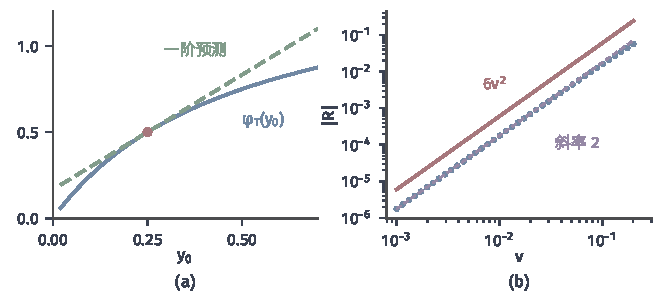
\includegraphics[width=112mm]{figures/06-differential-equations/01-ordinary-differential-equations/matplotlib/odesens-first-order/figure.pdf}
  \caption{Logistic方程的一阶预测，$T=\ln3$。(a)解映射$\varphi_T$（蓝）与红点处的一阶预测$\tfrac12+\tfrac43(y_0-\tfrac14)$（绿虚线）。(b)余项$\lvert R\rvert$随$v$的变化（蓝点），红线是上界$6v^2$，紫色虚线是斜率为$2$的参考线。}
  \label{fig:odesens-first-order}
\end{BookInlineFigure}

\subsection{初值导数}
\label{sec:odesens-initial-derivative}

只改变初值时$\bm{w}=\bm{0}$，变分方程齐次，解对$\bm{v}$线性。把$\bm{v}$依次取为$\mathbb{R}^{n}$的标准基，所得$n$个解排成一个矩阵，也就是解对初始状态的Jacobian矩阵
\begin{equation}
 \bm{S}(t)=\frac{\partial\bm{x}(t;\bm{x}_0)}{\partial\bm{x}_0}\in\mathbb{R}^{n\times n}.
 \label{eq:odesens-initial-jacobian}
\end{equation}
由式~\eqref{eq:odesens-variational}，它满足以单位矩阵为初值的线性系统
\begin{equation}
 \dot{\bm{S}}=\bm{A}(t)\bm{S},\qquad \bm{S}(t_0)=\bm{I}.
 \label{eq:odesens-initial-variational}
\end{equation}

这正是第~\ref{chap:linear-differential-systems}章的状态转移矩阵的定义方程。那里证明了$\bm{\Phi}(t,s)$对$t$满足该线性系统、$\bm{\Phi}(s,s)=\bm{I}$，并满足复合关系$\bm{\Phi}(t,s)\bm{\Phi}(s,r)=\bm{\Phi}(t,r)$。因此$\bm{S}(t)=\bm{\Phi}(t,t_0)$，只是这里的$\bm{A}(t)$来自沿解的线性化，$\bm{\Phi}$依赖于所选的轨迹。

\paragraph{水面上的小木棍}
想象在水流中放一根极短的小木棍，一端在参考点$\bm{x}_0$，另一端在$\bm{x}_0+\bm{v}$。水流带着小木棍前进，同时拉长、压短并转动它。$\bm{z}(t)=\bm{S}(t)\bm{v}$就是$t$时刻的小木棍。对应关系是：水流是右端$\bm{f}$，小木棍是切向量，$\bm{A}(t)$描述当前位置附近水流的局部拉伸与旋转。类比到有限长度就失效了，长木棍会弯曲，而$\bm{z}$永远是直的箭头。

把$\bm{S}(t)$作奇异值分解$\bm{S}=\bm{U}\bm{\Sigma}\bm{V}^{\top}$。单位球面上的初值方向被映成椭球面，最大奇异值$\sigma_{\max}$是一阶下最坏的放大倍数，相应的$\bm{V}$的列是最敏感的初值方向，$\bm{U}$的列是响应的方向。

\begin{example}[可以手算的二维系统]
\label{ex:odesens-planar}
考虑
\[
 \dot{x}_1=-x_1,\qquad \dot{x}_2=x_2+x_1^2,
\]
初值$(1,0)$。第一个方程给出$x_1(t)=\mathrm{e}^{-t}$，沿解的线性化系数是
\[
 \bm{A}(t)=\begin{bmatrix}-1&0\\2\mathrm{e}^{-t}&1\end{bmatrix}.
\]

按列解式~\eqref{eq:odesens-initial-variational}。第二列满足$\dot{s}_{1,2}=-s_{1,2}$、$\dot{s}_{2,2}=2\mathrm{e}^{-t}s_{1,2}+s_{2,2}$，初值$(0,1)$，于是
\[
 s_{1,2}=0,\qquad s_{2,2}=\mathrm{e}^{t}.
\]
第一列初值为$(1,0)$，由第一个方程得$s_{1,1}=\mathrm{e}^{-t}$，代入第二个方程，
\[
 \dot{s}_{2,1}=s_{2,1}+2\mathrm{e}^{-2t},\qquad s_{2,1}(0)=0.
\]

乘以积分因子$\mathrm{e}^{-t}$，得
\[
 \frac{\mathrm{d}}{\mathrm{d}t}\bigl(\mathrm{e}^{-t}s_{2,1}\bigr)=2\mathrm{e}^{-3t},
\]
积分后得到
\[
 s_{2,1}(t)=\tfrac23\bigl(\mathrm{e}^{t}-\mathrm{e}^{-2t}\bigr).
\]
取$t=\ln2$，参考解到达$(1/2,\,7/12)$，
\[
 \bm{S}(\ln2)=\begin{bmatrix}1/2&0\\7/6&2\end{bmatrix}.
\]

这个方程能显式求解，可以用来核对：从$(a,b)$出发，
\[
 x_1=a\mathrm{e}^{-t},\qquad x_2=\bigl(b+a^2/3\bigr)\mathrm{e}^{t}-\bigl(a^2/3\bigr)\mathrm{e}^{-2t}.
\]
对$(a,b)$在$(1,0)$处求导，结果与上式相同。$\bm{S}(\ln2)$的奇异值是$2.330$与$0.429$，最大奇异值比特征值$2$更大，这个差别来自$\bm{S}$非对称带来的转向。
\end{example}

图~\ref{fig:odesens-tangent-transport}把例~\ref{ex:odesens-planar}画了出来。红色小圆的两根基向量被$\bm{S}(\ln2)$带到蓝色箭头：$(1,0)$方向既缩短又转向，$(0,1)$方向被拉长两倍。半径$0.4$并不算小，真实的像（蓝色区域）和线性预测的椭圆（绿色虚线）已有肉眼可见的差别。

\begin{BookInlineFigure}
  \centering
  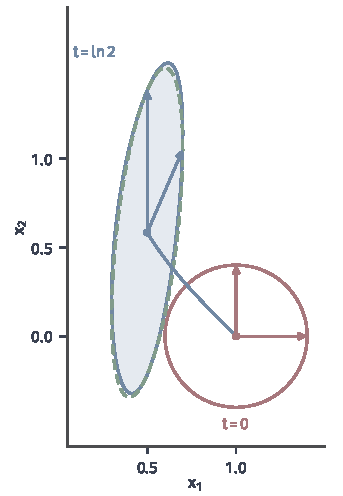
\includegraphics[width=58mm]{figures/06-differential-equations/01-ordinary-differential-equations/matplotlib/odesens-tangent-transport/figure.pdf}
  \caption{小圆随流的变形。方程为$\dot{x}_1=-x_1$，$\dot{x}_2=x_2+x_1^2$。红圆是$t=0$时以$(1,0)$为心、半径$0.4$的圆，蓝线是圆心的轨迹，浅蓝区域是$t=\ln2$时圆的真实像，绿色虚线是线性预测$\bm{x}(t)+\bm{S}(t)\bm{v}$的椭圆。红箭头是两根基向量，蓝箭头是它们在$\bm{S}(\ln2)$下的像。}
  \label{fig:odesens-tangent-transport}
\end{BookInlineFigure}

\paragraph{沿轨迹方向的导数}
自治方程有一个不用解方程就知道的解。对$\bm{f}(\bm{x}(t))$关于$t$求导，并用$\dot{\bm{x}}=\bm{f}(\bm{x})$，得到
\[
 \frac{\mathrm{d}}{\mathrm{d}t}\bm{f}(\bm{x}(t))=\bm{A}(t)\bm{f}(\bm{x}(t)).
\]
所以$\bm{f}(\bm{x}(t))$满足齐次变分方程，初值是$\bm{f}(\bm{x}_0)$。由线性方程的唯一性，
\begin{equation}
 \bm{S}(t)\,\bm{f}(\bm{x}_0)=\bm{f}(\bm{x}(t)).
 \label{eq:odesens-tangent-flow}
\end{equation}
含义是：把初值沿轨迹挪一点，只相当于把时间起点平移，$t$时刻的解也沿轨迹挪一点。

标量情形下，当$f(x_0)\neq0$时，式~\eqref{eq:odesens-tangent-flow}直接给出$S(t)=f(x(t))/f(x_0)$。在Logistic方程上，
\[
 S(\ln3)=\frac{\tfrac12\cdot\tfrac12}{\tfrac14\cdot\tfrac34}=\frac43,
\]
与例~\ref{ex:odesens-first-order}的积分结果一致。再继续到$t=2\ln3$，$x$从$1/2$增长到$3/4$，这一段的放大倍数是$(3/16)/(1/4)=3/4$，全程是$\tfrac43\cdot\tfrac34=1$，放大和压缩恰好抵消，这正是复合关系$\bm{\Phi}(t,s)\bm{\Phi}(s,r)=\bm{\Phi}(t,r)$的一个实例。

\paragraph{增长的$\bm{S}$不等于发散的轨迹}
Jacobian矩阵增长并不说明解跑远了。无阻尼摆$\dot{q}=p$、$\dot{p}=-\sin q$的轨道是封闭曲线，但周期依赖振幅。两条相邻轨道相位差随时间线性累积，$\bm{S}$的范数因而线性增长，见图~\ref{fig:odesens-pendulum-growth}。这里的增长来自相位的错开，不是轨道的分离，而轨迹全程有界。这再次说明，有限时间的一阶响应和长期行为是不同的问题。

\begin{BookInlineFigure}
  \centering
  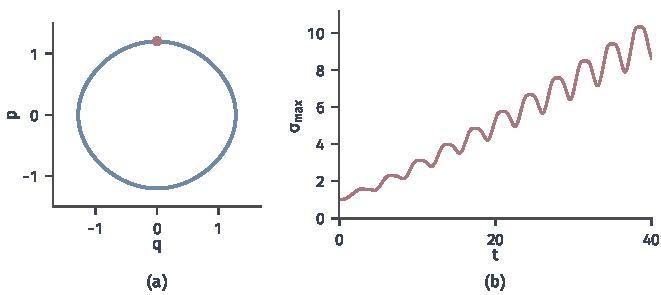
\includegraphics[width=112mm]{figures/06-differential-equations/01-ordinary-differential-equations/matplotlib/odesens-pendulum-growth/figure.pdf}
  \caption{无阻尼摆的初值Jacobian矩阵。(a)从红点$(q,p)=(0,1.2)$出发的封闭轨道。(b)式~\eqref{eq:odesens-initial-variational}数值积分得到的最大奇异值$\sigma_{\max}(t)$，在振荡中近似线性增长，$t=40$内从$1$升到约$10$，而轨道始终有界。}
  \label{fig:odesens-pendulum-growth}
\end{BookInlineFigure}

\subsection{参数导数}
\label{sec:odesens-parameter-derivative}

现在让参数变化。先取有限维参数$\bm{\theta}\in\mathbb{R}^{p}$，初值也可能依赖参数，写成$\bm{x}_0(\bm{\theta})$。把$\bm{w}$取遍标准基，方向导数排成矩阵
\begin{equation}
 \bm{P}(t)=\frac{\partial\bm{x}(t;\bm{\theta})}{\partial\bm{\theta}}\in\mathbb{R}^{n\times p}.
 \label{eq:odesens-parameter-jacobian}
\end{equation}
在式~\eqref{eq:odesens-variational}中$\bm{v}=(\partial_{\bm{\theta}}\bm{x}_0)\bm{w}$，于是$\bm{P}$满足
\begin{equation}
 \dot{\bm{P}}=\bm{A}(t)\bm{P}+\bm{B}(t),\qquad \bm{P}(t_0)=\partial_{\bm{\theta}}\bm{x}_0(\bm{\theta}).
 \label{eq:odesens-parameter-variational}
\end{equation}
与初值导数相比，多了非齐次项$\bm{B}(t)$：参数改变时，每一时刻的变化率都被额外推了一下。

这个线性方程的解由第~\ref{chap:linear-differential-systems}章的常数变易公式给出：
\begin{equation}
 \bm{P}(t)=\bm{\Phi}(t,t_0)\,\partial_{\bm{\theta}}\bm{x}_0+\int_{t_0}^{t}\bm{\Phi}(t,s)\bm{B}(s)\,\mathrm{d}s.
 \label{eq:odesens-parameter-formula}
\end{equation}
第一项是初值本身对参数的依赖，第二项是时刻$s$对变化率的推动再传播到$t$。结构和Gronwall上界完全对应，只是把放大因子的上界换成了真实的传播矩阵。

\begin{example}[增长率的导数]
\label{ex:odesens-parameter-derivative}
对$\dot{x}=\theta x(1-x)$，$\theta=1$，$x_0=1/4$，系数是
\[
 A(t)=1-2x(t),\qquad B(t)=x(t)(1-x(t)).
\]
初值不依赖参数，所以$P(0)=0$。式~\eqref{eq:odesens-parameter-variational}是$\dot{P}=(1-2x)P+x(1-x)$。

猜测$P=t\,x(1-x)$，即$P=tf(x)$，代入验证。由$\frac{\mathrm{d}}{\mathrm{d}t}f(x)=(1-2x)f(x)$，得到
\[
 \dot{P}=f(x)+t(1-2x)f(x)=x(1-x)+(1-2x)P,
\]
满足方程，且$P(0)=0$。这个结果也可以这样理解：解依赖$\theta t$，改变$\theta$相当于改变时间尺度。

在$t=\ln3$处，$x=1/2$，$P(\ln3)=\tfrac14\ln3\approx0.2747$。$\theta$增加$0.2$时，一阶预测的改变量是$0.0549$，例~\ref{ex:odesens-parameter-bound}中的真实差是$0.0547$，而Gronwall上界是$0.0901$。

若初值也依赖参数，比如$x_0(\theta)=\theta/4$，则$\partial_\theta x_0=1/4$，由式~\eqref{eq:odesens-parameter-formula}，
\[
 P(\ln3)=\frac43\cdot\frac14+\frac14\ln3\approx0.3333+0.2747=0.6080.
\]
前一项用了初值导数$S(\ln3)=4/3$。
\end{example}

图~\ref{fig:odesens-parameter-derivative}画出了$P(t)$。参数的影响在$x$中等时最大，$x$接近$0$或$1$时增长率的具体数值几乎不起作用。绿点是有限差分，它与变分方程的解重合。

\begin{BookInlineFigure}
  \centering
  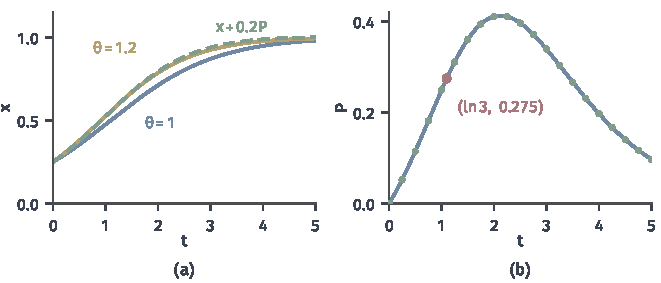
\includegraphics[width=112mm]{figures/06-differential-equations/01-ordinary-differential-equations/matplotlib/odesens-parameter-derivative/figure.pdf}
  \caption{参数导数。方程$\dot{x}=\theta x(1-x)$，$x_0=1/4$。(a)$\theta=1$（蓝）、$\theta=1.2$（黄）的解，绿色虚线是一阶预测$x+0.2P$。(b)$P(t)$的变分方程解（蓝）与有限差分（绿点），红点是$t=\ln3$处的值。}
  \label{fig:odesens-parameter-derivative}
\end{BookInlineFigure}

\paragraph{参数化的输入}
输入是一个函数，自由度无穷多。常见的做法是用有限个参数表示它，比如$\bm{g}(t)=\bm{g}(t;\bm{\theta})$，然后归入上面的计算。右端写成$\bm{f}(t,\bm{x},\bm{g}(t;\bm{\theta}))$，由链式法则，
\begin{equation}
 \bm{B}(t)=\partial_{\bm{g}}\bm{f}\bigl(t,\bm{x}(t),\bm{g}(t;\bm{\theta})\bigr)\,\partial_{\bm{\theta}}\bm{g}(t;\bm{\theta}).
 \label{eq:odesens-input-derivative}
\end{equation}
其余不变。定理~\ref{thm:odesens-differentiable}对$t$只要求可测，$\partial_{\bm{\theta}}\bm{g}$可以有跳变。

考虑$\dot{x}=-x+g(t)$，$x_0=0$，$t\in[0,2]$，$g$在$[0,1)$上取$\theta_1$，在$[1,2)$上取$\theta_2$，这里取$\theta_1=1$、$\theta_2=2$。此时$A=-1$，$\bm{B}(t)$在两段上分别是$(1,0)$与$(0,1)$，于是$P_j$分别解$\dot{P}_j=-P_j+B_j$。直接积分，
\[
 P_1(2)=\mathrm{e}^{-1}(1-\mathrm{e}^{-1})\approx0.2325,\qquad
 P_2(2)=1-\mathrm{e}^{-1}\approx0.6321.
\]
较早的输入经历了$\mathrm{e}^{-1}$的衰减，对末态的影响较小，图~\ref{fig:odesens-input-basis}(b)的折点就发生在切换时刻。

\begin{BookInlineFigure}
  \centering
  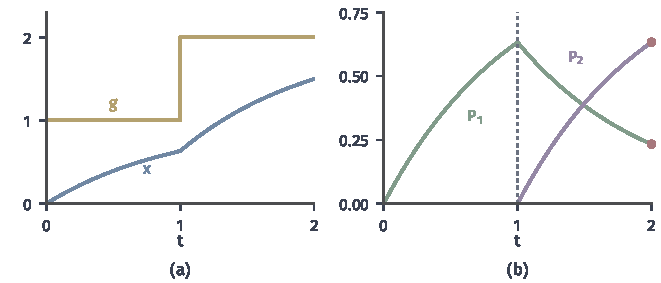
\includegraphics[width=112mm]{figures/06-differential-equations/01-ordinary-differential-equations/matplotlib/odesens-input-basis/figure.pdf}
  \caption{分段常值输入的参数导数。方程$\dot{x}=-x+g$，$x_0=0$。(a)输入$g$（黄）与解$x$（蓝），$\theta=(1,2)$。(b)参数导数$P_1$（绿）、$P_2$（紫），灰色虚线是切换时刻$t=1$，红点是$t=2$时的值。}
  \label{fig:odesens-input-basis}
\end{BookInlineFigure}

\section{解的流映射}
\label{sec:odesens-flow}

到现在为止我们盯着一条解和它附近的解。换一个视角：固定起止时刻，让所有初始状态同时运动。方向场上每一点都顺流而下，整个状态空间被搬动了一段。这个“搬动”本身是一个映射，前面得到的初值依赖、Jacobian矩阵都成为它的性质。

本节设$\bm{D}\subseteq\mathbb{R}\times\mathbb{R}^{n}$开，$\bm{f}:\bm{D}\to\mathbb{R}^{n}$连续，且$\partial_{\bm{x}}\bm{f}$在$\bm{D}$上存在并连续，这样过$\bm{D}$中每点的最大解都存在且唯一。时间可测时，把$\bm{f}$的条件换成定理~\ref{thm:odesens-differentiable}的条件，并把涉及时间导数的结论理解为几乎处处成立。

\begin{definition}[流映射]
\label{def:odesens-flow}
对时刻$s,t$，记$\bm{D}_{s,t}$为满足下述条件的$\bm{x}\in\mathbb{R}^{n}$的集合：$(s,\bm{x})\in\bm{D}$，且过$(s,\bm{x})$的最大解在时刻$t$有定义。在$\bm{D}_{s,t}$上定义\term{流映射}（flow map）
\begin{equation}
 \bm{\varphi}_{s,t}(\bm{x})=\text{过}(s,\bm{x})\text{的最大解在时刻}\ t\ \text{的值}.
 \label{eq:odesens-flow}
\end{equation}
\end{definition}

记号$\bm{\varphi}_{s,t}$保留了起止两个时刻。$\bm{D}_{s,t}$可能是真子集，甚至是空集，因为有些解活不到$t$。由定理~\ref{thm:odesens-local-lipschitz}，$\bm{D}_{s,t}$是开集，$\bm{\varphi}_{s,t}$在其上局部Lipschitz；由定理~\ref{thm:odesens-differentiable}，它连续可微，Jacobian矩阵是沿相应解的状态转移矩阵，
\begin{equation}
 \mathrm{D}\bm{\varphi}_{s,t}(\bm{x})=\bm{\Phi}(t,s).
 \label{eq:odesens-flow-jacobian}
\end{equation}
图~\ref{fig:odesens-flow-domain}是$\dot{x}=x^2$的流映射，它的定义域随$t$收缩。

\begin{BookInlineFigure}
  \centering
  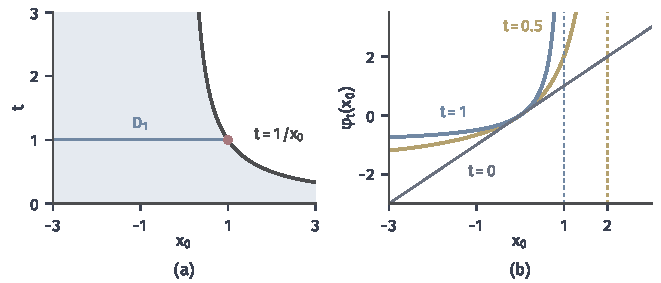
\includegraphics[width=112mm]{figures/06-differential-equations/01-ordinary-differential-equations/matplotlib/odesens-flow-domain/figure.pdf}
  \caption{流映射的定义域依赖时间。方程$\dot{x}=x^2$，$\varphi_t(x)=x/(1-tx)$。(a)浅蓝区域是$\{(x_0,t):t\geq0,\ tx_0<1\}$，深灰线是爆炸曲线$t=1/x_0$，蓝色水平线是$t=1$时的定义域$\bm{D}_1=(-\infty,1)$。(b)$\varphi_t$的图像，$t=0$是恒等映射（灰），$t=0.5$（黄）、$t=1$（蓝）在虚线处趋于无穷。}
  \label{fig:odesens-flow-domain}
\end{BookInlineFigure}

\subsection{局部可逆性}
\label{sec:odesens-flow-inverse}

解在唯一性条件下不会分叉也不会合并。所以从$s$走到$r$再走到$t$，应当等于直接走到$t$；从$s$走到$t$再走回来，应当回到原处。这是流映射的两条代数规则，图~\ref{fig:odesens-flow-composition}是它们的示意。

\begin{BookInlineFigure}
  \centering
  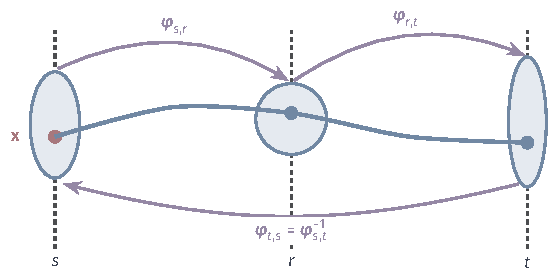
\includegraphics[width=93.4mm]{figures/06-differential-equations/01-ordinary-differential-equations/tikz/odesens-flow-composition/figure.pdf}
  \caption{流映射的复合与逆。三条虚线是时刻$s,r,t$上的状态空间，浅蓝区域是一小块初值及其像，蓝线是过红点的解。上方两个映射相继作用等于$\bm{\varphi}_{s,t}$，下方的映射$\bm{\varphi}_{t,s}$把终点送回起点。}
  \label{fig:odesens-flow-composition}
\end{BookInlineFigure}

\begin{theorem}[流映射的复合与局部可逆性]
\label{thm:odesens-flow}
在本节的条件下：
\begin{enumerate}
 \item 对$(s,\bm{x})\in\bm{D}$，有$\bm{\varphi}_{s,s}(\bm{x})=\bm{x}$；
 \item 若$\bm{x}\in\bm{D}_{s,r}$且$\bm{\varphi}_{s,r}(\bm{x})\in\bm{D}_{r,t}$，则$\bm{x}\in\bm{D}_{s,t}$，且
 \begin{equation}
  \bm{\varphi}_{r,t}\bigl(\bm{\varphi}_{s,r}(\bm{x})\bigr)=\bm{\varphi}_{s,t}(\bm{x});
  \label{eq:odesens-flow-composition}
 \end{equation}
 \item $\bm{\varphi}_{s,t}:\bm{D}_{s,t}\to\bm{D}_{t,s}$是$C^1$双射，逆映射是$\bm{\varphi}_{t,s}$，且Jacobian矩阵处处可逆，
 \begin{equation}
  \mathrm{D}\bm{\varphi}_{t,s}\bigl(\bm{\varphi}_{s,t}(\bm{x})\bigr)=\bigl[\mathrm{D}\bm{\varphi}_{s,t}(\bm{x})\bigr]^{-1}.
  \label{eq:odesens-flow-inverse}
 \end{equation}
\end{enumerate}
\end{theorem}

\begin{proof}
第一条是定义。

第二条用唯一性。过$(s,\bm{x})$的最大解在时刻$r$的值是$\bm{\varphi}_{s,r}(\bm{x})$，所以它也是过$(r,\bm{\varphi}_{s,r}(\bm{x}))$的解。由最大解的唯一性，这两条最大解相同。后者在$t$有定义，前者也就在$t$有定义，两边的值相等。

第三条是第二条的特例。设$\bm{x}\in\bm{D}_{s,t}$，$\bm{y}=\bm{\varphi}_{s,t}(\bm{x})$。过$(t,\bm{y})$的最大解就是过$(s,\bm{x})$的最大解，它在$s$有定义且值为$\bm{x}$，所以$\bm{y}\in\bm{D}_{t,s}$，且$\bm{\varphi}_{t,s}(\bm{y})=\bm{x}$。交换$s,t$得到另一个方向。两个映射都是$C^1$的，对恒等映射$\bm{\varphi}_{t,s}\circ\bm{\varphi}_{s,t}$用链式法则，就得到式~\eqref{eq:odesens-flow-inverse}。
\end{proof}

这里没有用到反函数定理，逆映射是由“反向求解”直接造出来的，并且在整个$\bm{D}_{s,t}$上有定义，不只在一点附近。之所以仍称为局部可逆性，是因为$\bm{D}_{s,t}$通常不是整个空间，定理并不假定解全局存在。

\paragraph{自治方程与单参数局部流}
当$\bm{f}$不显含时间时，若$\bm{x}(t)$是解，平移后的$\bm{x}(t+c)$也是解。于是$\bm{\varphi}_{s,t}$只依赖时长$t-s$，记$\bm{\varphi}_{t}=\bm{\varphi}_{0,t}$。式~\eqref{eq:odesens-flow-composition}变成
\begin{equation}
 \bm{\varphi}_{t}\circ\bm{\varphi}_{r}=\bm{\varphi}_{t+r}.
 \label{eq:odesens-local-flow}
\end{equation}
等式在式~\eqref{eq:odesens-flow-composition}的定义域条件下成立，所以$\{\bm{\varphi}_t\}$称为\term{单参数局部流}（local one-parameter flow）。若所有解全局存在，它才是定义在整个空间上的单参数群。

对$\dot{x}=x^2$，$\varphi_t(x)=x/(1-tx)$，直接代入，
\[
 \varphi_t\bigl(\varphi_r(x)\bigr)=\frac{x/(1-rx)}{1-tx/(1-rx)}=\frac{x}{1-(t+r)x}=\varphi_{t+r}(x),
\]
要求$rx<1$且$tx/(1-rx)<1$。当$t,r>0$时，这等价于$(t+r)x<1$；$\varphi_{-t}$是$\varphi_t$在定义域上的逆。

非自治方程不能这样简写。对$\dot{x}=tx$，$\varphi_{s,t}(x)=x\,\mathrm{e}^{(t^2-s^2)/2}$。从$0$走到$1$乘以$\mathrm{e}^{1/2}$，再用同一规律“走一个单位时间”乘以$\mathrm{e}^{1/2}$，得到的$\mathrm{e}$并不等于从$0$到$2$的倍数$\mathrm{e}^{2}$。第二段时间的起点是$1$，规律已经变了，所以必须记下起止两个时刻。

\paragraph{没有唯一性时会怎样}
可逆性来自轨道不合并。方程$\dot{x}=-2\,\mathrm{sgn}(x)\sqrt{\lvert x\rvert}$在$x=0$处不Lipschitz。正向解唯一：右端单调递减，式~\eqref{eq:odesens-one-sided}成立且$\mu=0$，由引理~\ref{lem:odesens-one-sided}，两条解的距离不增，所以正向唯一。解是
\[
 x(t)=\mathrm{sgn}(x_0)\bigl(\max\{\sqrt{\lvert x_0\rvert}-t,\,0\}\bigr)^2.
\]

所有$\lvert x_0\rvert\leq t^2$的轨道在时刻$t$都已并入$0$，见图~\ref{fig:odesens-merging}。$\varphi_1$把整个$[-1,1]$压成一点，不是单射，没有逆映射，这正是反向解不唯一的表现。

\begin{BookInlineFigure}
  \centering
  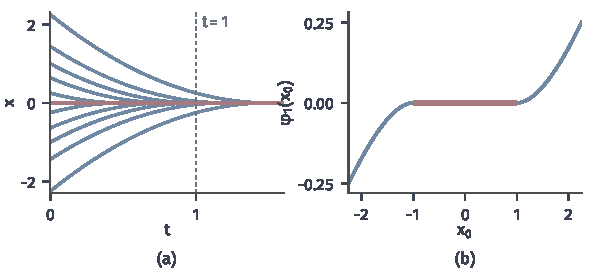
\includegraphics[width=100mm]{figures/06-differential-equations/01-ordinary-differential-equations/matplotlib/odesens-merging/figure.pdf}
  \caption{轨道合并破坏可逆性。方程$\dot{x}=-2\,\mathrm{sgn}(x)\sqrt{\lvert x\rvert}$。(a)各初值的轨道在有限时间并入红色的零解。(b)$t=1$时的解映射，红色线段$[-1,1]$被压成一点。}
  \label{fig:odesens-merging}
\end{BookInlineFigure}

\subsection{体积变化}
\label{sec:odesens-volume}

流映射把一小块初始区域搬到别处，体积会变吗？线性映射的体积倍数是行列式的绝对值，而流映射在一小块上近似线性，Jacobian矩阵是$\bm{S}(t)$。于是要看的是$J(t)=\det\bm{S}(t)$怎样随时间变化。

\paragraph{直观}
考虑很短的时间$h$，由式~\eqref{eq:odesens-initial-variational}有$\bm{S}(t+h)\approx(\bm{I}+h\bm{A}(t))\bm{S}(t)$。而
\[
 \det(\bm{I}+h\bm{A})=1+h\operatorname{tr}\bm{A}+O(h^2),
\]
所以每一小段时间内体积的相对变化率是$\operatorname{tr}\bm{A}$，也就是右端的散度。放在水流的图景中，散度是某点处水流的“膨胀率”：散度为正的地方，流体微团在膨胀。把这个观察写成精确的等式，就是\term{Liouville公式}（Liouville formula）。

\begin{lemma}[Liouville公式]
\label{lem:odesens-liouville}
设$\bm{S}$满足式~\eqref{eq:odesens-initial-variational}，其中$\bm{A}$可积。则$J=\det\bm{S}$绝对连续，几乎处处满足$\dot{J}=\operatorname{tr}\bm{A}(t)\,J$，于是
\begin{equation}
 J(t)=\exp\int_{t_0}^{t}\operatorname{tr}\bm{A}(s)\,\mathrm{d}s>0.
 \label{eq:odesens-liouville}
\end{equation}
\end{lemma}

\begin{proof}
行列式是矩阵元素的多项式，$\bm{S}$绝对连续，所以$J$绝对连续。矩阵函数的微分给出
\[
 \mathrm{d}\det{}_{\bm{S}}(\bm{E})=\operatorname{tr}\bigl(\operatorname{adj}(\bm{S})\bm{E}\bigr),
\]
这个公式对奇异矩阵也成立，可参考\BookChapterRef{chap:matrix-differentiation}{卷二第21章“矩阵函数的微分”}。代入$\dot{\bm{S}}=\bm{A}\bm{S}$，
\[
 \dot{J}=\operatorname{tr}\bigl(\operatorname{adj}(\bm{S})\bm{A}\bm{S}\bigr).
\]

用迹的循环性，再用$\bm{S}$与其古典伴随的乘积等于$\det(\bm{S})\bm{I}$，
\[
 \dot{J}=\operatorname{tr}\bigl(\bm{A}\bm{S}\operatorname{adj}(\bm{S})\bigr)=\operatorname{tr}(\bm{A})\,J.
\]
这是标量线性方程，$J(t_0)=1$，解就是式~\eqref{eq:odesens-liouville}。
\end{proof}

沿解，$\operatorname{tr}\bm{A}(t)$正是右端在$(t,\bm{x}(t))$处的散度$\nabla\cdot\bm{f}$，这里的散度只对状态变量求。式~\eqref{eq:odesens-liouville}中$J>0$说明流映射保持定向，也就不会出现把区域翻折的情况。

三个手算例子可以用来核对。常系数线性方程$\dot{\bm{x}}=\bm{A}\bm{x}$有
\[
 \det\mathrm{e}^{t\bm{A}}=\mathrm{e}^{t\operatorname{tr}\bm{A}}.
\]
例~\ref{ex:odesens-planar}的散度是$-1+1=0$，相应的行列式是$\tfrac12\cdot2=1$。Logistic方程是一维的，“体积”就是长度，放大倍数$\exp\int(1-2x)\,\mathrm{d}t$等于$4/3$，与$S(\ln3)$相同。

\begin{theorem}[体积变化公式]
\label{thm:odesens-volume}
在本节的条件下，设$\bm{W}\subseteq\bm{D}_{s,t}$是可测集。则
\begin{equation}
 \operatorname{vol}\bigl(\bm{\varphi}_{s,t}(\bm{W})\bigr)=\int_{\bm{W}}\exp\Bigl(\int_{s}^{t}\nabla\cdot\bm{f}\bigl(r,\bm{\varphi}_{s,r}(\bm{x})\bigr)\,\mathrm{d}r\Bigr)\mathrm{d}\bm{x}.
 \label{eq:odesens-volume}
\end{equation}
特别地，若$\bm{f}$的定义域$\bm{D}$上$\nabla\cdot\bm{f}\equiv0$，则流映射保持体积。反过来，若流映射对任意$s,t$和任意小球都保持体积，则$\nabla\cdot\bm{f}\equiv0$。
\end{theorem}

\begin{proof}
由定理~\ref{thm:odesens-flow}，$\bm{\varphi}_{s,t}$是开集之间的$C^1$双射，且Jacobian矩阵可逆。换元公式给出
\[
 \operatorname{vol}\bigl(\bm{\varphi}_{s,t}(\bm{W})\bigr)=\int_{\bm{W}}\bigl\lvert\det\mathrm{D}\bm{\varphi}_{s,t}(\bm{x})\bigr\rvert\,\mathrm{d}\bm{x}.
\]
这个公式及测度论背景可参考\BookChapterRef{chap:pushforward-measures}{卷四第9章“推前测度”}。把式~\eqref{eq:odesens-flow-jacobian}、式~\eqref{eq:odesens-liouville}代入，即得式~\eqref{eq:odesens-volume}，绝对值因$J>0$可去。

散度恒为零时，被积函数恒为$1$，体积保持。反过来，设某点$(s,\bm{x})$处$\nabla\cdot\bm{f}>0$（负的情形相同）。由连续性，$(s,\bm{x})$附近散度为正，取小球$\bm{W}$和很短的时间，使轨道段留在这个邻域内，则式~\eqref{eq:odesens-volume}的指数中积分为正，体积严格增大，矛盾。
\end{proof}

定理的条件都起作用。解的唯一性保证$\bm{\varphi}_{s,t}$单射，否则换元公式就不再有意义，图~\ref{fig:odesens-merging}的压缩映射便是反例。$\bm{f}$关于状态$C^1$保证了$\mathrm{D}\bm{\varphi}$连续。结论仅对$\bm{W}\subseteq\bm{D}_{s,t}$成立，爆炸的解所在的点不在其中。

图~\ref{fig:odesens-volume-change}比较了三种流。例~\ref{ex:odesens-planar}的流把正方形拉成细长曲边四边形，面积不变。阻尼振子$\dot{q}=p$、$\dot{p}=-q-\tfrac12p$的散度是$-\tfrac12$，面积按$\mathrm{e}^{-t/2}$缩小，边长$0.5$的正方形面积$0.25$，$t=2$时为$0.25\,\mathrm{e}^{-1}\approx0.092$。

\begin{BookInlineFigure}
  \centering
  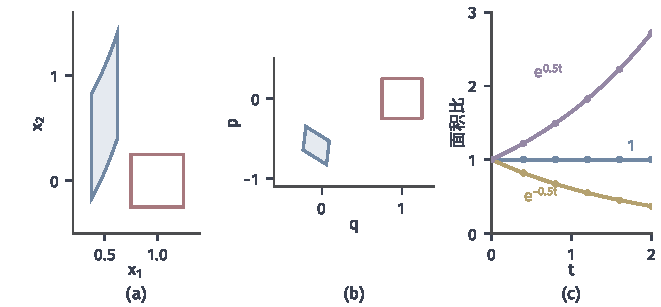
\includegraphics[width=112mm]{figures/06-differential-equations/01-ordinary-differential-equations/matplotlib/odesens-volume-change/figure.pdf}
  \caption{面积随流的变化。红框是初始正方形，浅蓝区域是它的像。(a)$\dot{x}_1=-x_1$、$\dot{x}_2=x_2+x_1^2$，$t=\ln2$，散度为零。(b)$\dot{q}=p$、$\dot{p}=-q-\tfrac12p$，$t=2$，散度为$-\tfrac12$。(c)面积比随时间的变化：线是式~\eqref{eq:odesens-liouville}，点是由多边形面积算出的数值；蓝、黄分别对应(a)(b)，紫色对应$\dot{\bm{x}}=\tfrac14\bm{x}$。}
  \label{fig:odesens-volume-change}
\end{BookInlineFigure}

\paragraph{沿轨迹的值与密度}
一块墨水随水流运动，某个粒子携带的值沿轨迹不变，而墨水的密度要随微团的伸缩改变，这是两件不同的事。设质量密度$p_s$在流映射下被推到$p_t$，质量守恒要求对任意$\bm{W}$有
\[
 \int_{\bm{\varphi}_{s,t}(\bm{W})}p_t(\bm{y})\,\mathrm{d}\bm{y}=\int_{\bm{W}}p_s(\bm{x})\,\mathrm{d}\bm{x}.
\]
左边用换元公式换回$\bm{x}$，比较被积函数，得到
\begin{equation}
 p_t\bigl(\bm{\varphi}_{s,t}(\bm{x})\bigr)=\frac{p_s(\bm{x})}{\det\mathrm{D}\bm{\varphi}_{s,t}(\bm{x})}.
 \label{eq:odesens-density}
\end{equation}
取对数并对$t$求导，由式~\eqref{eq:odesens-liouville}，沿轨迹有
\[
 \frac{\mathrm{d}}{\mathrm{d}t}\ln p_t\bigl(\bm{x}(t)\bigr)=-\nabla\cdot\bm{f}\bigl(t,\bm{x}(t)\bigr).
\]
膨胀的地方密度下降。

以Logistic方程为例。$x_0$在$[0.1,0.4]$上均匀分布，密度$p_0=10/3$。$T=\ln3$时，$x_0=1/4$被送到$1/2$，Jacobian是$4/3$，所以
\[
 p_T(1/2)=\frac{10/3}{4/3}=2.5.
\]
图~\ref{fig:odesens-density-push}对比了这个公式与样本直方图。右侧的$x_0$被拉伸得少，密度更高。式~\eqref{eq:odesens-density}是第~\ref{chap:transport-equations}章输运方程的基础，随机变量经可逆映射变换时的密度公式也是同一件事，可参考\BookChapterRef{chap:random-sampling-integration}{卷七第14章“随机采样与积分计算”}。

\begin{BookInlineFigure}
  \centering
  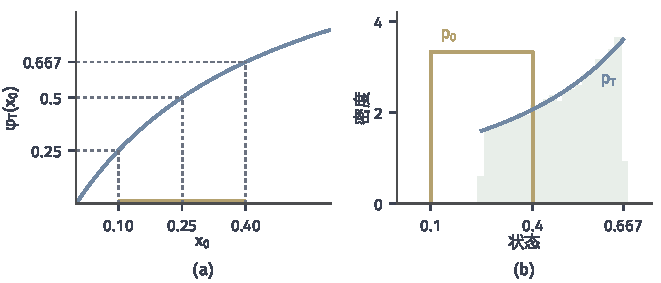
\includegraphics[width=112mm]{figures/06-differential-equations/01-ordinary-differential-equations/matplotlib/odesens-density-push/figure.pdf}
  \caption{流映射推动密度。方程$\dot{x}=x(1-x)$，$T=\ln3$。(a)流映射把黄色区间$[0.1,0.4]$送到$[0.25,0.667]$。(b)均匀密度$p_0$（黄）被推成$p_T$（蓝），绿色直方图来自$40000$个由固定种子生成的样本。}
  \label{fig:odesens-density-push}
\end{BookInlineFigure}

\subsection{Hamilton流}
\label{sec:odesens-hamilton}

有一类重要的方程，散度为零是结构带来的，不用逐个验证。力学系统的状态由位置$\bm{q}$和动量$\bm{p}$组成，运动由一个函数决定。摆的总能量是$H(q,p)=\tfrac12p^2+1-\cos q$，而摆的方程$\dot{q}=p$、$\dot{p}=-\sin q$恰好是
\[
 \dot{q}=\partial_pH,\qquad \dot{p}=-\partial_qH.
\]
这个形式可以推广。

\begin{definition}[Hamilton方程]
\label{def:odesens-hamilton}
设$H(t,\bm{q},\bm{p})$是定义在$\mathbb{R}\times\mathbb{R}^{m}\times\mathbb{R}^{m}$的开集上的函数，关于$t$连续，关于$(\bm{q},\bm{p})$二阶连续可微，且这些偏导数连续。称
\begin{equation}
 \dot{\bm{q}}=\nabla_{\bm{p}}H(t,\bm{q},\bm{p}),\qquad
 \dot{\bm{p}}=-\nabla_{\bm{q}}H(t,\bm{q},\bm{p})
 \label{eq:odesens-hamilton}
\end{equation}
为\term{Hamilton方程}（Hamilton's equations），$H$称为Hamilton函数（Hamiltonian），$(\bm{q},\bm{p})\in\mathbb{R}^{2m}$所在空间称为\term{相空间}（phase space），相应的流映射称为\term{Hamilton流}（Hamiltonian flow）。
\end{definition}

$H\in C^2$正好保证右端关于状态$C^1$，本节前面的结论全部适用。下面两条性质分别回答体积和能量。

\begin{theorem}[Hamilton流的体积与能量]
\label{thm:odesens-hamilton}
在定义~\ref{def:odesens-hamilton}的条件下，Hamilton流在其定义域内保持相空间体积（$H$可以显含时间）。若$H$还关于$t$连续可微，沿Hamilton方程的解有
\begin{equation}
 \frac{\mathrm{d}}{\mathrm{d}t}H\bigl(t,\bm{q}(t),\bm{p}(t)\bigr)=\partial_tH\bigl(t,\bm{q}(t),\bm{p}(t)\bigr).
 \label{eq:odesens-energy}
\end{equation}
特别地，$H$不显含时间时，$H$沿解不变。
\end{theorem}

\begin{proof}
相空间中的散度是
\[
 \nabla\cdot\bm{f}=\sum_{i=1}^{m}\Bigl(\frac{\partial}{\partial q_i}\frac{\partial H}{\partial p_i}-\frac{\partial}{\partial p_i}\frac{\partial H}{\partial q_i}\Bigr)=0,
\]
最后一步用了$H\in C^2$时混合偏导相等。由定理~\ref{thm:odesens-volume}，流保持体积。

由链式法则及式~\eqref{eq:odesens-hamilton}，
\[
 \frac{\mathrm{d}H}{\mathrm{d}t}=\partial_tH+\langle\nabla_{\bm{q}}H,\dot{\bm{q}}\rangle+\langle\nabla_{\bm{p}}H,\dot{\bm{p}}\rangle=\partial_tH+\langle\nabla_{\bm{q}}H,\nabla_{\bm{p}}H\rangle-\langle\nabla_{\bm{p}}H,\nabla_{\bm{q}}H\rangle.
\]
后两项相消，即得式~\eqref{eq:odesens-energy}。
\end{proof}

显含时间时，能量可以变化。受迫振子取$H=\tfrac12p^2+\tfrac12q^2-g(t)q$，方程是$\dot{q}=p$、$\dot{p}=-q+g(t)$，式~\eqref{eq:odesens-energy}的右端是$-\dot{g}(t)q$。取$g(t)=t$，$q(0)=0$，$p(0)=1$，解是$q=t$、$p=1$，代入$H$得
\[
 H(t,t,1)=\tfrac12+\tfrac12t^2-t^2=\tfrac12-\tfrac12t^2.
\]
其导数是$-t$，正好等于$-\dot{g}q=-t$。此时能量不守恒，但相空间体积仍然保持。

图~\ref{fig:odesens-hamilton-flow}是摆的相空间。在无阻尼情形下，半径$0.35$的圆被剪切成细长的月牙形，沿能量等值线运动，面积在$t=0,3,6$时都是$0.3848$。加上阻尼$\dot{p}=-\sin q-0.4p$后，方程不再是Hamilton方程，散度为$-0.4$，面积按$\mathrm{e}^{-0.4t}$缩小到$0.1159$与$0.0349$。

\begin{BookInlineFigure}
  \centering
  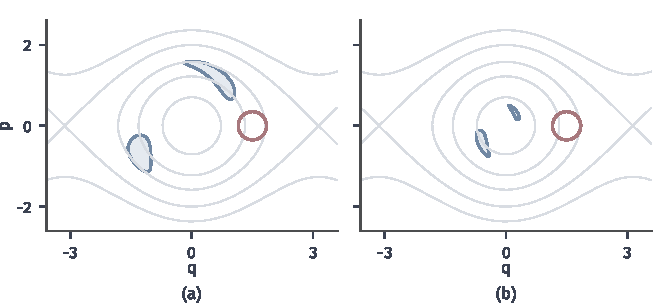
\includegraphics[width=112mm]{figures/06-differential-equations/01-ordinary-differential-equations/matplotlib/odesens-hamilton-flow/figure.pdf}
  \caption{摆的相空间。灰线是能量$H=\tfrac12p^2+1-\cos q$的等值线，红圆是初始区域，浅蓝区域是$t=3$和$t=6$时的像。(a)无阻尼，面积保持。(b)阻尼系数$0.4$，面积按$\mathrm{e}^{-0.4t}$收缩，区域离开能量等值线向内运动。}
  \label{fig:odesens-hamilton-flow}
\end{BookInlineFigure}

体积保持和能量守恒是两个不同的性质，互相不能推出，见表~\ref{tab:odesens-volume-energy}。

\begin{BookInlineTable}
  \centering
  \caption{体积保持与能量守恒的对比。“能量”指表中给定的函数。}
  \label{tab:odesens-volume-energy}
  \begin{tabular}{p{52mm}p{14mm}p{30mm}}
    \toprule
    系统 & 体积 & 能量 \\
    \midrule
    自治Hamilton方程 & 保持 & 守恒 \\
    显含时间的Hamilton方程 & 保持 & 按$\partial_tH$变化 \\
    阻尼摆 & 收缩 & $H$单调不增 \\
    $\dot{q}=(1+q^2)p$，$\dot{p}=-(1+q^2)q$ & 不保持 & $q^2+p^2$守恒 \\
    \bottomrule
  \end{tabular}
\end{BookInlineTable}

表中最后一行的散度是$2qp$，非零，但
\[
 \frac{\mathrm{d}}{\mathrm{d}t}(q^2+p^2)=2(1+q^2)(qp-pq)=0.
\]
这样的方程沿能量面运动，却不保持体积。

Hamilton流的这两条性质是后面几处的基础。第~\ref{chap:hamilton-jacobi-equations}章由Hamilton方程构造特征线，用它们重建场。构造采样提议时，流的可逆性和体积保持让接受概率的计算得以简化，可参考\BookChapterRef{chap:discrete-time-stochastic-processes}{卷九第3章“离散时间随机过程”}。两者都不说明解会靠拢，能量不变也不能推出渐近收敛。

\section{伴随方程}
\label{sec:odesens-adjoint}

设参数有$p$个，而我们只关心由解算出的一个数，比如终点状态的某个函数。用式~\eqref{eq:odesens-parameter-variational}求梯度，就要解一个$n\times p$的矩阵方程，相当于$p$个线性系统。$p$很大时这难以承受，而我们要的只是一个数对$p$个参数的导数。能不能只解一次方程？

\paragraph{主要思想}
设目标函数同时含终端项和沿途的运行项：
\begin{equation}
 J(\bm{\theta})=\psi\bigl(\bm{x}(T),\bm{\theta}\bigr)+\int_{t_0}^{T}\ell\bigl(t,\bm{x}(t),\bm{\theta}\bigr)\,\mathrm{d}t,
 \label{eq:odesens-objective}
\end{equation}
其中$\bm{x}$解$\dot{\bm{x}}=\bm{f}(t,\bm{x},\bm{\theta})$，$\bm{x}(t_0)=\bm{x}_0(\bm{\theta})$。沿方向$\bm{w}$求导，$\bm{z}=\bm{P}\bm{w}$解变分方程，得到
\[
 \mathrm{D}J[\bm{w}]=\langle\nabla_{\bm{x}}\psi,\bm{z}(T)\rangle+\langle\nabla_{\bm{\theta}}\psi,\bm{w}\rangle+\int_{t_0}^{T}\bigl(\langle\nabla_{\bm{x}}\ell,\bm{z}\rangle+\langle\nabla_{\bm{\theta}}\ell,\bm{w}\rangle\bigr)\,\mathrm{d}t.
\]
麻烦的是$\bm{z}$，每换一个$\bm{w}$都要重解。

解决办法来自一个恒等式。设$\bm{z}$解$\dot{\bm{z}}=\bm{A}\bm{z}$，$\bm{\lambda}$解$\dot{\bm{\lambda}}=-\bm{A}^{\top}\bm{\lambda}$，则
\[
 \frac{\mathrm{d}}{\mathrm{d}t}\langle\bm{\lambda},\bm{z}\rangle=\langle-\bm{A}^{\top}\bm{\lambda},\bm{z}\rangle+\langle\bm{\lambda},\bm{A}\bm{z}\rangle=0.
\]
配对$\langle\bm{\lambda},\bm{z}\rangle$沿时间不变。如果$\bm{\lambda}$在终点等于目标的梯度，那么
\[
 \langle\nabla\psi,\bm{z}(T)\rangle=\langle\bm{\lambda}(t_0),\bm{z}(t_0)\rangle.
\]
于是问题转移到了起点：$\bm{z}(t_0)$是已知的。代价是$\bm{\lambda}$的条件给在终点，要从$T$反向解回$t_0$，图~\ref{fig:odesens-adjoint-scheme}是这个结构的示意。

\begin{BookInlineFigure}
  \centering
  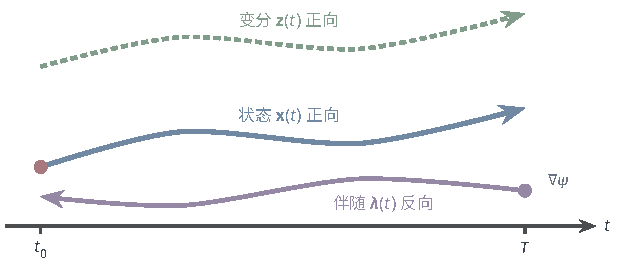
\includegraphics[width=105.2mm]{figures/06-differential-equations/01-ordinary-differential-equations/tikz/odesens-adjoint-scheme/figure.pdf}
  \caption{伴随计算的结构。状态$\bm{x}$从红色初值正向求解。变分$\bm{z}$（绿色虚线）也是正向的，每个方向都要解一次，伴随方法用不到它。伴随$\bm{\lambda}$（紫）从终点条件$\nabla\psi$出发反向求解，只解一次。配对$\langle\bm{\lambda},\bm{z}\rangle$在无运行项、无输入项时沿时间不变。}
  \label{fig:odesens-adjoint-scheme}
\end{BookInlineFigure}

一般情形多了非齐次项，只要在$\bm{\lambda}$的方程里补上运行项的梯度。在变分方程上演算，就得到下面的定理。

\begin{theorem}[伴随表示]
\label{thm:odesens-adjoint}
设$\bm{f}$满足定理~\ref{thm:odesens-differentiable}的条件，$\bm{x}_0(\bm{\theta})$、$\psi$连续可微，$\ell$对$t$可测、对$(\bm{x},\bm{\theta})$连续可微，且其导数在管道内被可积函数控制。设$\bm{A},\bm{B}$由式~\eqref{eq:odesens-coefficients}定义。令$\bm{\lambda}:[t_0,T]\to\mathbb{R}^{n}$是反向线性问题
\begin{equation}
 \dot{\bm{\lambda}}=-\bm{A}(t)^{\top}\bm{\lambda}-\nabla_{\bm{x}}\ell\bigl(t,\bm{x}(t),\bm{\theta}\bigr),\qquad
 \bm{\lambda}(T)=\nabla_{\bm{x}}\psi\bigl(\bm{x}(T),\bm{\theta}\bigr)
 \label{eq:odesens-adjoint}
\end{equation}
的解。则$J$在$\bm{\theta}$处可微，且
\begin{equation}
 \begin{aligned}
 \nabla J(\bm{\theta})={}&\nabla_{\bm{\theta}}\psi+\bigl[\partial_{\bm{\theta}}\bm{x}_0(\bm{\theta})\bigr]^{\top}\bm{\lambda}(t_0)\\
 &+\int_{t_0}^{T}\bigl[\bm{B}(t)^{\top}\bm{\lambda}(t)+\nabla_{\bm{\theta}}\ell\bigr]\,\mathrm{d}t.
 \end{aligned}
 \label{eq:odesens-adjoint-gradient}
\end{equation}
\end{theorem}

\begin{proof}
可微性由定理~\ref{thm:odesens-differentiable}、$\psi$的可微性以及该定理证明第四步那样的控制收敛论证得到，方向导数正是前面写出的$\mathrm{D}J[\bm{w}]$。式~\eqref{eq:odesens-adjoint}是系数可积的线性方程，在$[t_0,T]$上有唯一的绝对连续解。

设$\bm{z}$解方向$\bm{w}$的变分方程~\eqref{eq:odesens-variational}，起点取$(\partial_{\bm{\theta}}\bm{x}_0)\bm{w}$。计算配对的导数，$\bm{A}$的项相消，几乎处处有
\[
 \frac{\mathrm{d}}{\mathrm{d}t}\langle\bm{\lambda},\bm{z}\rangle=-\langle\nabla_{\bm{x}}\ell,\bm{z}\rangle+\langle\bm{\lambda},\bm{B}\bm{w}\rangle.
\]

从$t_0$到$T$积分，并代入$\bm{\lambda}(T)=\nabla_{\bm{x}}\psi$，移项得
\[
 \langle\nabla_{\bm{x}}\psi,\bm{z}(T)\rangle+\int_{t_0}^{T}\langle\nabla_{\bm{x}}\ell,\bm{z}\rangle\,\mathrm{d}t=\langle\bm{\lambda}(t_0),\bm{z}(t_0)\rangle+\int_{t_0}^{T}\langle\bm{\lambda},\bm{B}\bm{w}\rangle\,\mathrm{d}t.
\]
左边正是$\mathrm{D}J[\bm{w}]$中含$\bm{z}$的部分。代回$\mathrm{D}J[\bm{w}]$，右端对$\bm{w}$线性，读出系数就是式~\eqref{eq:odesens-adjoint-gradient}。
\end{proof}

称$\bm{\lambda}$为\term{伴随变量}（adjoint variable），式~\eqref{eq:odesens-adjoint}为\term{伴随方程}（adjoint equation）。式~\eqref{eq:odesens-adjoint-gradient}的各项对应目标导数的三个来源：含$\nabla_{\bm{\theta}}\psi$与$\nabla_{\bm{\theta}}\ell$的项是目标函数显含参数的部分；含$\bm{\lambda}(t_0)$的项是初值对参数的依赖；含$\bm{B}$的项是右端对参数的依赖。

\paragraph{$\bm{\lambda}$的含义}
无运行项时，比较式~\eqref{eq:odesens-adjoint}与式~\eqref{eq:odesens-initial-variational}，得到
\begin{equation}
 \bm{\lambda}(t)=\bm{\Phi}(T,t)^{\top}\nabla_{\bm{x}}\psi\bigl(\bm{x}(T)\bigr).
 \label{eq:odesens-adjoint-pullback}
\end{equation}
也就是说，$\bm{\lambda}(t)$是目标函数对时刻$t$状态的梯度：如果在时刻$t$把状态推动$\bm{v}$，目标函数的一阶变化是$\langle\bm{\lambda}(t),\bm{v}\rangle$。带运行项时含义相同，只是目标函数换成从$t$到$T$的累计。变分$\bm{z}$回答“推一下起点，后面怎么变”，伴随$\bm{\lambda}$回答“后面的目标，对前面每一刻有多敏感”，一个前传，一个后传。

\begin{example}[Logistic方程上的配对]
\label{ex:odesens-adjoint-logistic}
继续$\dot{x}=\theta x(1-x)$，$\theta=1$，$x_0=1/4$，$T=\ln3$，取$J=x(T)$，即$\psi(x)=x$，$\ell=0$。伴随方程是$\dot{\lambda}=-(1-2x)\lambda$，$\lambda(T)=1$。

记$f(x)=x(1-x)$。对$1/f(x(t))$求导，得到
\[
 \frac{\mathrm{d}}{\mathrm{d}t}\,\frac{1}{f(x)}=-\frac{1-2x}{f(x)}.
\]
所以$1/f(x(t))$满足伴随方程的齐次形式，配上终端条件，得
\[
 \lambda(t)=\frac{f(x(T))}{f(x(t))}.
\]
代入数据，$f(x(T))=1/4$，所以$\lambda(0)=\dfrac{1/4}{3/16}=\dfrac43$，这就是初值导数$S(T)$，与式~\eqref{eq:odesens-adjoint-pullback}一致。

对$\theta$的导数，$B(t)=f(x(t))$，所以
\[
 \lambda(t)B(t)=f(x(T))=\frac14\quad\text{（对所有}\ t\text{）}.
\]
积分得到$\partial_\theta J=\tfrac14\ln3\approx0.2747$，与例~\ref{ex:odesens-parameter-derivative}的$P(\ln3)$相同。
\end{example}

图~\ref{fig:odesens-adjoint-pairing}(a)中，$z=S(t)$从$1$升到$4/3$，$\lambda$从$4/3$降到$1$，乘积始终是$4/3$，这正是配对不变的数值表现。(b)显示伴随变量和被积函数的具体形状。

\begin{BookInlineFigure}
  \centering
  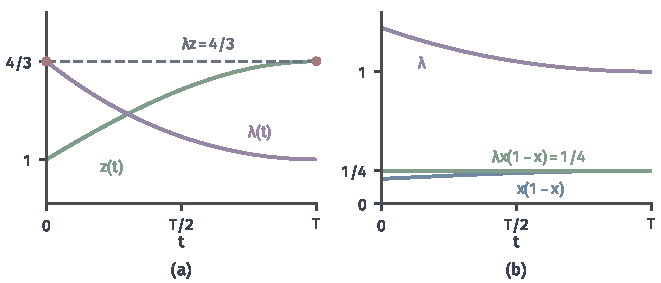
\includegraphics[width=112mm]{figures/06-differential-equations/01-ordinary-differential-equations/matplotlib/odesens-adjoint-pairing/figure.pdf}
  \caption{Logistic方程上的变分与伴随，$x_0=1/4$，$T=\ln3$，$J=x(T)$，数值积分得到。(a)前向的$z(t)=S(t)$（绿）与反向的$\lambda(t)$（紫），灰色虚线是乘积$\lambda z\equiv4/3$。红点是$\lambda(0)=z(T)=4/3$。(b)$\lambda$（紫）、$B=x(1-x)$（蓝）及其乘积（绿），乘积恒为$1/4$。}
  \label{fig:odesens-adjoint-pairing}
\end{BookInlineFigure}

\begin{example}[三个来源逐项核对]
\label{ex:odesens-adjoint-three}
取$\dot{x}=\theta x$，$x(0)=\theta$，$T=1$，
\[
 J(\theta)=\int_0^1\Bigl(x(t)+\frac12\theta^2\Bigr)\mathrm{d}t.
\]
解是$x=\theta\mathrm{e}^{\theta t}$，直接积分得$J=\mathrm{e}^{\theta}-1+\tfrac12\theta^2$，所以$J'(1)=\mathrm{e}+1$。

用伴随计算，取$\theta=1$。这里$\psi=0$，$\ell=x+\tfrac12\theta^2$，$A=1$，$B=x=\mathrm{e}^{t}$。伴随方程$\dot{\lambda}=-\lambda-1$、$\lambda(1)=0$的解是
\[
 \lambda(t)=\mathrm{e}^{1-t}-1.
\]

三项贡献依次是：
\[
 \begin{aligned}
 \text{初值：}&\ \partial_\theta x_0\,\lambda(0)=1\cdot(\mathrm{e}-1)=\mathrm{e}-1,\\
 \text{右端：}&\ \int_0^1\lambda B\,\mathrm{d}t=\int_0^1\bigl(\mathrm{e}-\mathrm{e}^{t}\bigr)\mathrm{d}t=1,\\
 \text{目标：}&\ \int_0^1\partial_\theta\ell\,\mathrm{d}t=\int_0^1\theta\,\mathrm{d}t=1.
 \end{aligned}
\]
相加得$\mathrm{e}+1$，与直接求导的结果相同。
\end{example}

\paragraph{计算过程}
下面把伴随方法写成计算过程，并同时在第~\ref{sec:odesens-parameter-derivative}节的分段输入例子上执行：$\dot{x}=-x+g(t)$，$x_0=0$，$T=2$，$g$在$[0,1)$、$[1,2)$上分别取$\theta_1=1$、$\theta_2=2$，目标是$J=\tfrac12x(2)^2$。

\needspace{6\baselineskip}
\paragraph{变量}
需要的量是：
\begin{itemize}
 \item 状态轨迹$\bm{x}(t)\in\mathbb{R}^{n}$，要保存下来或能够重新算出，供反向求解时使用；
 \item 伴随变量$\bm{\lambda}(t)\in\mathbb{R}^{n}$；
 \item 累积梯度$\bm{G}(t)\in\mathbb{R}^{p}$，表示$[t,T]$这段时间已经计入的梯度贡献。
\end{itemize}

\paragraph{初始化}
参数$\bm{\theta}$、初值$\bm{x}_0(\bm{\theta})$给定。例中$\bm{\theta}=(1,2)$，$x_0=0$，$\partial_{\bm{\theta}}x_0=\bm{0}$。

\needspace{6\baselineskip}
\paragraph{计算步骤}
\begin{enumerate}
 \item \emph{正向求解状态}，得到$\bm{x}(t)$，$t\in[t_0,T]$。例中逐段积分，
 \[
  x(1)=1-\mathrm{e}^{-1}=0.63212,\qquad x(2)=2+\bigl(x(1)-2\bigr)\mathrm{e}^{-1}=1.49679.
 \]

 \item \emph{设置终端条件}。令
 \[
  \bm{\lambda}(T)=\nabla_{\bm{x}}\psi(\bm{x}(T),\bm{\theta}),\qquad\bm{G}(T)=\bm{0}.
 \]
 例中$\lambda(2)=x(2)=1.49679$。

 \item \emph{反向求解伴随}。由式~\eqref{eq:odesens-adjoint}从$T$积到$t_0$，同时累积
 \[
  \dot{\bm{G}}=-\bigl[\bm{B}(t)^{\top}\bm{\lambda}(t)+\nabla_{\bm{\theta}}\ell\bigr].
 \]
 例中$A=-1$，无运行项，方程为$\dot{\lambda}=\lambda$，所以$\lambda(t)=x(2)\mathrm{e}^{t-2}$，
 \[
  \lambda(1)=0.55064,\qquad\lambda(0)=0.20257.
 \]

 \item \emph{合成梯度}。由式~\eqref{eq:odesens-adjoint-gradient}，
 \[
  \nabla J=\bm{G}(t_0)+\nabla_{\bm{\theta}}\psi+\bigl[\partial_{\bm{\theta}}\bm{x}_0\bigr]^{\top}\bm{\lambda}(t_0).
 \]
 例中$B$在$[0,1)$上为$(1,0)$，在$[1,2)$上为$(0,1)$，初值项为零，
 \[
  \partial_{\theta_1}J=\int_0^1\lambda\,\mathrm{d}t=0.34807,\qquad
  \partial_{\theta_2}J=\int_1^2\lambda\,\mathrm{d}t=0.94615.
 \]
\end{enumerate}

积分到$t_0$，计算结束。最终得到$\nabla J(1,2)=(0.34807,\,0.94615)$。用第~\ref{sec:odesens-parameter-derivative}节的$P_j(2)$核对，$\partial_{\theta_j}J=x(2)P_j(2)$，分别是$1.49679\times0.23254$与$1.49679\times0.63212$，结果相同。

图~\ref{fig:odesens-adjoint-gradient}把输入分成$20$段。一次反向积分给出全部$20$个偏导数，红点是逐分量差分的结果，最大差约$2\times10^{-7}$。越晚的输入对$J$的影响越大，因为$\lambda(t)$在靠近$T$时最大。

\begin{BookInlineFigure}
  \centering
  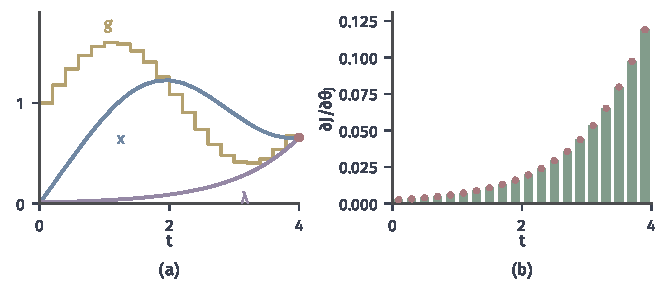
\includegraphics[width=112mm]{figures/06-differential-equations/01-ordinary-differential-equations/matplotlib/odesens-adjoint-gradient/figure.pdf}
  \caption{一次反向求解给出全部偏导数。方程$\dot{x}=-x+g$，$x_0=0$，$g$在$[0,4]$上分$20$段取常值（黄），$J=\tfrac12x(4)^2$。(a)状态$x$（蓝）与伴随$\lambda(t)=x(4)\mathrm{e}^{t-4}$（紫），红点是终端值。(b)绿色柱是伴随计算的$20$个偏导数，红点是逐分量中心差分。}
  \label{fig:odesens-adjoint-gradient}
\end{BookInlineFigure}

\paragraph{代价与失效情形}
表~\ref{tab:odesens-forward-adjoint}比较了前向与反向两种求导方式，其中$p$是参数个数，$k$是目标函数的个数。

\begin{BookInlineTable}
  \centering
  \caption{前向变分与反向伴随的代价对比。线性系统指沿同一条轨迹的$n$维线性初值问题。}
  \label{tab:odesens-forward-adjoint}
  \begin{tabular}{p{22mm}p{38mm}p{38mm}}
    \toprule
    & 前向变分 & 反向伴随 \\
    \midrule
    线性系统个数 & $p$个 & $k$个 \\
    是否保存轨迹 & 不需要，与状态同步 & 需要保存或重算 \\
    适合的情形 & 参数少、目标多 & 参数多、目标少 \\
    额外产出 & 完整的$\bm{P}(t)$ & 每一时刻的$\bm{\lambda}(t)$ \\
    \bottomrule
  \end{tabular}
\end{BookInlineTable}

伴随的主要代价是轨迹的存储。反向积分时要用到$\bm{A}(t)$，也就要用到$\bm{x}(t)$，长时间问题要在内存和重算之间权衡。$\bm{\lambda}$的大小也受放大因子控制：由式~\eqref{eq:odesens-adjoint-pullback}，
\[
 \lVert\bm{\lambda}(t)\rVert_2\leq\lVert\bm{\Phi}(T,t)\rVert_2\lVert\nabla\psi\rVert_2.
\]
敏感的问题里梯度本身就很大。

数值计算时还要注意，定理给的是连续问题的梯度。把伴随方程离散后算出的结果，一般不等于对离散格式求导的结果，两者只在步长趋于零时一致。定理的光滑性条件也不能省：右端在解经过的地方有$\lvert x\rvert$那样的折点时，$J$可能不可微。

得到梯度只是第一步，用它更新参数属于优化算法，可参考\BookChapterRef{chap:first-order-methods}{卷五第6章“一阶方法”}。当未知量是控制函数而不是有限维参数时，最优性条件需要更多工具，可参考\BookChapterRef{chap:continuous-time-optimal-control}{卷十第6章“连续时间最优控制”}。

\section{本章小结}
\label{sec:odesens-summary}

章首的问题是：把$x_0$改成$0.26$，或把增长率改$20\%$，$t=\ln3$时的值会差多少？现在有三种回答。Gronwall上界告诉我们，两种改变的影响分别不超过$0.01\,\mathrm{e}^{\ln3}=0.03$和$0.1$。变分方程给出一阶值$\tfrac43\times0.01=0.0133$与$0.0549$，后者与真实差$0.0547$很接近。若只需要一个目标对很多参数的梯度，伴随方程用一次反向求解就能得到。

四个工具输出的量不同，见表~\ref{tab:odesens-tools}。

\begin{BookInlineTable}
  \centering
  \caption{本章工具的对比。结论都针对给定解附近的紧时间段。}
  \label{tab:odesens-tools}
  \begin{tabular}{p{16mm}p{24mm}p{27mm}p{28mm}}
    \toprule
    工具 & 输出 & 主要条件 & 不能回答 \\
    \midrule
    Gronwall估计 & 曲线距离的上界 & 状态Lipschitz，系数可积 & 差的方向；长期趋势 \\
    变分方程 & 一阶响应$\bm{S}$、$\bm{P}$ & 对状态、参数$C^1$，导数有可积上界 & 大扰动；非光滑处 \\
    流映射 & 复合、逆、体积变化 & 解唯一，$C^1$ & 定义域外的解；长期轨道 \\
    伴随方程 & 目标函数的梯度 & 同变分方程，目标$C^1$ & 整个$\bm{P}(t)$；控制函数的最优性 \\
    \bottomrule
  \end{tabular}
\end{BookInlineTable}

几个相近的概念要分清。连续依赖只说解差随数据差趋于零；Lipschitz依赖给出速度，需要右端局部Lipschitz；可微依赖给出一阶系数，需要右端$C^1$，这三者一层比一层强，且不能由弱推强，$\dot{x}=-x\ln\lvert x\rvert$和$\dot{x}=\lvert x\rvert$分别是分界的反例。积分范数适合度量右端关于输入Lipschitz时的输入差，非线性增长时要限制输入的取值或改用更强的范数。残差和放大因子分别来自求解器和方程。

所有结论都是有限时间的。常数$\mathrm{e}^{\Lambda(T)}$可以很保守，也不说明长时间下解是靠拢还是分离，长期稳定需要卷九的额外结构和条件。第~\ref{chap:ode-numerical-methods}章的全局误差分析将回用本章的扰动估计，第~\ref{chap:transport-equations}章的输运方程回用流映射和体积变化。


\chapter{初值问题的数值求解}
\label{chap:ode-numerical-methods}

考虑初值问题$\dot{x}=x(1-x)$，$x(0)=0.2$，我们想知道$x(1)$是多少。这个方程恰好能分离变量，答案是$\mathrm{e}/(\mathrm{e}+4)\approx0.404610$。可是只要右端稍微复杂一点，比如添上一项$\sin(tx)$，第~\ref{chap:ordinary-differential-equations}章的解法就用不上了。第~\ref{chap:ode-existence-continuation}章的定理告诉我们解存在且唯一，却没有告诉我们它在$t=1$时等于多少。

计算机只能保存有限个数、做有限次运算，所以真正能算的是解曲线上有限个时刻的近似值。把曲线换成一串数之后，马上面临三个问题：从一个时刻到下一个时刻究竟怎样走；每一步的小偏差累积到终点时有多大；步长由什么决定，能不能让程序自己选。

本章按这三个问题展开。前三节建立时间离散的语言，再给出Euler方法和Runge--Kutta方法，用同一个初值问题比较它们的误差与计算量。第~\ref{sec:odenum-error-convergence}节在有限区间上证明，一步误差经过怎样的条件才累积成确定阶数的全局误差。

高阶方法并不总是最好的选择。第~\ref{sec:odenum-stiff}节的快慢系统里，真正限制步长的是数值扰动的稳定性，而不是精度，这引出了隐式方法。第~\ref{sec:odenum-adaptive}节让程序按局部误差估计自动调节步长，并说明这样的估计能保证什么、不能保证什么。

本章始终讨论有限时间区间，并假定真解在整个区间上存在。上面的方程$\dot{x}=x(1-x)$贯穿全章：它是非线性的，手算只需几位小数，又有闭式解可以用来核对结果。

\section{时间离散}
\label{sec:odenum-time-discretization}

连续的解是一条曲线，算法只能交出有限个数。这有限个数应该是什么，怎样一个接一个地产生，又该拿什么标准评价它们？

\paragraph{时间网格与一步更新}
固定初值问题
\begin{equation}
 \dot{\bm{x}}(t)=\bm{f}(t,\bm{x}(t)),\qquad \bm{x}(t_0)=\bm{x}_0,
 \label{eq:odenum-ivp}
\end{equation}
并假定它在有限区间$[t_0,t_0+T]$上有唯一解$\bm{x}(t)$，$\bm{x}(t)\in\mathbb{R}^{n}$。存在、唯一与延拓的条件见第~\ref{chap:ode-existence-continuation}章。

把区间等分成$N$份，步长$h=T/N$，得到\term{时间网格}（time grid）
\begin{equation}
 t_k=t_0+kh,\qquad k=0,1,\ldots,N.
 \label{eq:odenum-grid}
\end{equation}
数值解是一串向量$\bm{x}^{(0)},\bm{x}^{(1)},\ldots,\bm{x}^{(N)}$，其中$\bm{x}^{(k)}$用来近似$\bm{x}(t_k)$。上标带括号表示网格编号，不是导数的阶数。

真解自身满足一个“一步”关系。在$[t_k,t_{k+1}]$上积分方程，得到
\begin{equation}
 \bm{x}(t_{k+1})=\bm{x}(t_k)+\int_{t_k}^{t_{k+1}}\bm{f}(s,\bm{x}(s))\,\mathrm{d}s.
 \label{eq:odenum-integral-step}
\end{equation}
右端的积分依赖这一步内部尚不知道的解，所以不能直接算。本章所有方法都在回答同一件事：只用当前已知的量，怎样近似这个积分。

用流映射的话说，式~\eqref{eq:odenum-integral-step}就是
\[
 \bm{x}(t_{k+1})=\bm{\varphi}_{t_k,t_{k+1}}\bigl(\bm{x}(t_k)\bigr),
\]
其中$\bm{\varphi}_{s,t}(\bm{y})$表示时刻$s$从$\bm{y}$出发的解在时刻$t$的值。流映射一般算不出来，于是用一个可计算的映射代替它。

\begin{definition}[一步方法]
 \label{def:odenum-one-step}
 \term{一步方法}（one-step method）由一族映射$\bm{\Psi}_h(t,\cdot)$给出，步长为$h$时按
 \begin{equation}
  \bm{x}^{(k+1)}=\bm{\Psi}_h\bigl(t_k,\bm{x}^{(k)}\bigr),\qquad k=0,1,\ldots,N-1
  \label{eq:odenum-one-step}
 \end{equation}
 从$\bm{x}^{(0)}$逐步计算。$\bm{\Psi}_h$只依赖当前的$t_k$、$\bm{x}^{(k)}$、步长和右端$\bm{f}$，不依赖更早的网格值。
\end{definition}

\paragraph{连续曲线、网格值与插值结果}
离散之后手里有三种不同的对象，它们很容易被混为一谈。图~\ref{fig:odenum-grid-values}把它们画在一起：蓝线是真解，是我们想知道却拿不到的函数；绿点是网格值，是算法实际产生的全部输出；绿色虚线是把相邻网格值连起来的折线，它是另加的一条规则，并不来自方程。

\begin{BookInlineFigure}
 \centering
 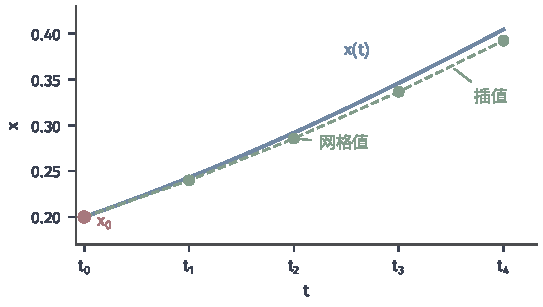
\includegraphics[width=92mm]{figures/06-differential-equations/01-ordinary-differential-equations/matplotlib/odenum-grid-values/figure.pdf}
 \caption{初值问题$\dot{x}=x(1-x)$，$x(0)=0.2$的三种对象。蓝线是真解，红点是初值，绿点是某个一步方法在步长$h=1/4$下给出的网格值，绿色虚线是对网格值作的分段线性插值。}
 \label{fig:odenum-grid-values}
\end{BookInlineFigure}

讨论误差时必须先说清比较的是哪一种对象。本章的误差都指网格点上$\bm{x}^{(k)}$与$\bm{x}(t_k)$的差。

网格点之间的值需要另外的插值规则，插值规则有自己的误差。若方法在网格上很精确，而插值只用分段线性，那么网格点之间的误差由插值决定，只有$h^2$的量级，精确的网格值也就白费了。

\paragraph{三种误差的来源}
数值解离真解有多远，来自三个不同的环节。第一，出发点可能不准：$0.2$在二进制中是无限循环小数，存进计算机时已经有舍入，初值本身也可能来自测量。第二，一步更新只是对式~\eqref{eq:odenum-integral-step}的近似。第三，每一步的运算有舍入误差，隐式方法（第~\ref{sec:odenum-stiff}节）还要加上内部方程没有解到底的误差。

用$\bm{\delta}^{(0)}$记初值误差，用$\bm{\delta}^{(k)}$（$k\geq1$）记第$k$步的计算误差，把实际算出的序列写成
\begin{equation}
 \bm{x}^{(0)}=\bm{x}_0+\bm{\delta}^{(0)},\qquad
 \bm{x}^{(k+1)}=\bm{\Psi}_h\bigl(t_k,\bm{x}^{(k)}\bigr)+\bm{\delta}^{(k+1)}.
 \label{eq:odenum-computed}
\end{equation}
理想算术且初值精确时，所有$\bm{\delta}^{(k)}$都为零。

第二个环节需要单独定义。关键是把出发点放在真解上，这样它只反映更新规则本身的缺陷，不混入以前积累的偏差。

\begin{definition}[局部截断误差与全局误差]
 \label{def:odenum-errors}
 设$\bm{x}(t)$是式~\eqref{eq:odenum-ivp}的解。第$k+1$步的\term{局部截断误差}（local truncation error）是从真解出发走一步与真解的差，
 \begin{equation}
  \bm{\ell}^{(k+1)}=\bm{\Psi}_h\bigl(t_k,\bm{x}(t_k)\bigr)-\bm{x}(t_{k+1}).
  \label{eq:odenum-local-error}
 \end{equation}
 \term{全局误差}（global error）是实际算出的网格值与真解的差，
 \begin{equation}
  \bm{e}^{(k)}=\bm{x}^{(k)}-\bm{x}(t_k).
  \label{eq:odenum-global-error}
 \end{equation}
\end{definition}

注意$\bm{\ell}^{(k+1)}$没有除以步长，它就是一步之内产生的偏差。两种误差的关系可以直接写出来。把式~\eqref{eq:odenum-computed}代入$\bm{e}^{(k+1)}$，再加减$\bm{\Psi}_h(t_k,\bm{x}(t_k))$，得到
\begin{equation}
 \bm{e}^{(k+1)}
 =\underbrace{\bm{\Psi}_h\bigl(t_k,\bm{x}^{(k)}\bigr)-\bm{\Psi}_h\bigl(t_k,\bm{x}(t_k)\bigr)}_{\text{旧误差的传播}}
 +\bm{\ell}^{(k+1)}+\bm{\delta}^{(k+1)}.
 \label{eq:odenum-error-split}
\end{equation}
每步的全局误差等于“上一步误差被更新规则放大或缩小的结果”，加上本步新产生的截断误差和计算误差。图~\ref{fig:odenum-three-errors}画出了这三个环节的位置。

\begin{BookInlineFigure}
 \centering
 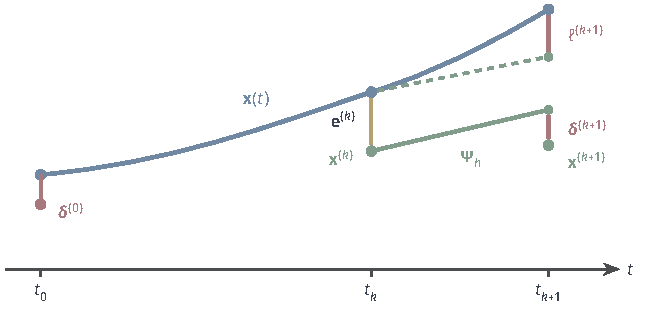
\includegraphics[width=109mm]{figures/06-differential-equations/01-ordinary-differential-equations/tikz/odenum-three-errors/figure.pdf}
 \caption{误差分解的一步。蓝线是真解，红点标出初值误差$\bm{\delta}^{(0)}$；在$t_{k+1}$处，从真解点$\bm{x}(t_k)$按规则$\bm{\Psi}_h$走一步，落点与真解之差是局部截断误差$\bm{\ell}^{(k+1)}$；从算出的$\bm{x}^{(k)}$走一步（绿色），旧误差$\bm{e}^{(k)}$被传播，再叠加计算误差$\bm{\delta}^{(k+1)}$后得到$\bm{x}^{(k+1)}$。}
 \label{fig:odenum-three-errors}
\end{BookInlineFigure}

\paragraph{残差不能代替误差}
既然真解满足方程，一个诱人的检验是把近似解代回方程，看方程满足得好不好。这种检验要分两种情况看。

如果代入的是离散格式本身，得到的永远是零。网格值正是按式~\eqref{eq:odenum-one-step}算出来的，无论$h$多大，它都严格满足自己的递推，所以离散方程的残差不提供任何信息。

如果代入的是连续的插值函数$\tilde{\bm{x}}(t)$，就可以定义\term{残差}（residual）
\[
 \bm{r}(t)=\dot{\tilde{\bm{x}}}(t)-\bm{f}\bigl(t,\tilde{\bm{x}}(t)\bigr).
\]
残差小说明$\tilde{\bm{x}}$是一个“被轻轻推过的方程”的解，但两个方程的解相差多少，取决于方程本身怎样放大扰动。

下面的两个方程真解都是$\cos t$，只差一个符号。取$\sigma=\pm5$，初值问题为
\[
 \dot{x}=\sigma(x-\cos t)-\sin t,\qquad x(0)=1.
\]
设近似函数$\tilde{x}$从同一初值出发，残差恒为$r=10^{-3}$。

记$d(t)=\tilde{x}(t)-\cos t$，两式相减得到关于差的方程：
\[
 \dot{d}=\sigma d+r,\qquad d(0)=0.
\]
解这个常系数线性方程，得到
\[
 d(t)=\frac{r}{\sigma}\bigl(\mathrm{e}^{\sigma t}-1\bigr).
\]

当$t=2$时，$\sigma=-5$给出$\lvert d\rvert\approx2\times10^{-4}$，比残差还小。$\sigma=5$给出$\lvert d\rvert\approx4.4$，是解本身量级的好几倍。图~\ref{fig:odenum-residual-gap}展示了这一差别：残差完全相同，误差相差四个多数量级。

\begin{BookInlineFigure}
 \centering
 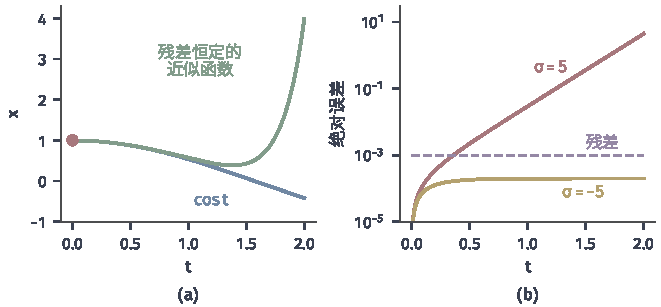
\includegraphics[width=112mm]{figures/06-differential-equations/01-ordinary-differential-equations/matplotlib/odenum-residual-gap/figure.pdf}
 \caption{残差相同而误差不同。(a)$\sigma=5$时，蓝线为真解$\cos t$，绿线为残差恒为$10^{-3}$的近似函数，二者很快分开。(b)绝对误差的对数图：紫色虚线是残差，红线和黄线分别是$\sigma=5$与$\sigma=-5$时的误差$\lvert d(t)\rvert$。}
 \label{fig:odenum-residual-gap}
\end{BookInlineFigure}

所以评价数值解时，要把初值误差、一步截断误差和每步计算误差分别记录，再结合误差的传播规律估计全局误差。这正是后面各节要做的事，传播规律由第~\ref{sec:odenum-error-convergence}节给出。


\section{Euler方法}
\label{sec:odenum-euler}

式~\eqref{eq:odenum-integral-step}的积分里，被积函数在这一步内部未知。最朴素的办法是假装它在这一步内不变，取起点的值。这样得到的方法是什么样，一步偏差多大，走完整个区间又要算多少次？

\paragraph{主要思想}
方向场在每个点$(t,\bm{x})$上给出一个速度$\bm{f}(t,\bm{x})$。站在当前点，读一次速度，沿这个方向走$h$的时间，到达新位置后再读一次，这就是\term{显式Euler方法}（explicit Euler method）。它像顺水漂流时每隔一段时间才看一眼水流方向：两次观察之间，方向按上一次的读数保持不变。类比的界限在于：真实的漂流者一直被水流带动，折线在两次读数之间却完全不看水流。

积分的说法与此相同。用$\bm{f}(t_k,\bm{x}^{(k)})$代替式~\eqref{eq:odenum-integral-step}中的被积函数，积分变成长度$h$乘以这个常向量，得到
\begin{equation}
 \bm{x}^{(k+1)}=\bm{x}^{(k)}+h\,\bm{f}\bigl(t_k,\bm{x}^{(k)}\bigr).
 \label{eq:odenum-euler}
\end{equation}

“显式”是指新值已经写在等号左边，右端只用旧值，代入即得。图~\ref{fig:odenum-euler-polygon}是这样得到的折线：每段都沿所在点的方向场切出去。真解沿方向场连续弯曲，折线每走一段才改一次方向，所以总是落在真解的一侧或另一侧。步长缩小后，改方向更频繁，折线更贴近真解。

\begin{BookInlineFigure}
 \centering
 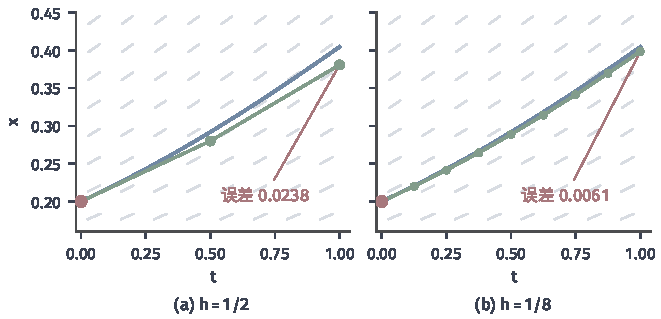
\includegraphics[width=112mm]{figures/06-differential-equations/01-ordinary-differential-equations/matplotlib/odenum-euler-polygon/figure.pdf}
 \caption{显式Euler折线与方向场。灰色短线是$\dot{x}=x(1-x)$的方向场，蓝线为$x(0)=0.2$的真解，绿线和绿点为数值解。(a)$h=1/2$；(b)$h=1/8$。红色标注是$t=1$处的绝对误差。}
 \label{fig:odenum-euler-polygon}
\end{BookInlineFigure}

\paragraph{计算过程}
下面用贯穿全章的初值问题逐步演示，数据为
\begin{equation}
 \dot{x}=x(1-x),\qquad x(0)=0.2,\qquad T=1.
 \label{eq:odenum-running}
\end{equation}
分离变量可得真解，它用来核对数值结果：
\begin{equation}
 x(t)=\frac{1}{1+4\mathrm{e}^{-t}}.
 \label{eq:odenum-running-exact}
\end{equation}
取$h=1/2$，于是$N=2$，手算两步即可走完。

\needspace{6\baselineskip}
\paragraph{变量}
\begin{itemize}
 \item $\bm{x}^{(k)}\in\mathbb{R}^{n}$：第$k$个网格点的数值解。
 \item $t_k$：当前时刻。
 \item $\bm{s}^{(k)}\in\mathbb{R}^{n}$：当前点读到的斜率。
\end{itemize}

\paragraph{初始化}
把数值解初始化为初值，时刻初始化为起点，步长和步数由区间决定：
\[
 \bm{x}^{(0)}=\bm{x}_0,\qquad t_0\text{给定},\qquad h=T/N.
\]
例中
\[
 x^{(0)}=0.2,\qquad t_0=0,\qquad h=0.5,\qquad N=2.
\]

\needspace{6\baselineskip}
\paragraph{每轮更新}
对$k=0,1,\ldots,N-1$依次执行：
\begin{enumerate}
 \item \textbf{读取斜率。}计算
 \[
  \bm{s}^{(k)}=\bm{f}\bigl(t_k,\bm{x}^{(k)}\bigr).
 \]
 例中第一轮
 \[
  s^{(0)}=0.2\times(1-0.2)=0.16.
 \]
 \item \textbf{沿斜率走一步。}由式~\eqref{eq:odenum-euler}计算
 \[
  \bm{x}^{(k+1)}=\bm{x}^{(k)}+h\,\bm{s}^{(k)},\qquad t_{k+1}=t_k+h.
 \]
 例中第一轮
 \[
  x^{(1)}=0.2+0.5\times0.16=0.28,\qquad t_1=0.5.
 \]
 例中第二轮先读斜率，再走一步：
 \[
  s^{(1)}=0.28\times0.72=0.2016,\qquad x^{(2)}=0.28+0.5\times0.2016=0.3808.
 \]
 \item \textbf{停止。}当$k+1=N$时结束。例中$k+1=2$，退出循环。
\end{enumerate}
最终得到网格值$\bm{x}^{(0)},\ldots,\bm{x}^{(N)}$。例中$x^{(2)}=0.3808$，而由式~\eqref{eq:odenum-running-exact}，$x(1)\approx0.404610$，误差约为$-0.0238$。

\paragraph{局部误差}
偏差从何而来？按定义~\ref{def:odenum-errors}，把真解代入一步更新。设$\bm{x}(t)$二次连续可微，含积分余项的Taylor公式给出
\[
 \bm{x}(t_{k+1})=\bm{x}(t_k)+h\dot{\bm{x}}(t_k)+\int_{t_k}^{t_{k+1}}(t_{k+1}-s)\ddot{\bm{x}}(s)\,\mathrm{d}s.
\]
真解满足$\dot{\bm{x}}(t_k)=\bm{f}(t_k,\bm{x}(t_k))$，这一项正好是Euler方法走的那一步，相减后只剩余项。于是显式Euler方法的局部截断误差是
\begin{equation}
 \bm{\ell}^{(k+1)}=-\int_{t_k}^{t_{k+1}}(t_{k+1}-s)\ddot{\bm{x}}(s)\,\mathrm{d}s.
 \label{eq:odenum-euler-local}
\end{equation}
权函数$t_{k+1}-s$在这一步上的积分是$h^2/2$，取范数得到局部误差界
\begin{equation}
 \bigl\lVert\bm{\ell}^{(k+1)}\bigr\rVert_2\leq\frac{h^2}{2}\max_{t\in[t_0,t_0+T]}\bigl\lVert\ddot{\bm{x}}(t)\bigr\rVert_2.
 \label{eq:odenum-euler-local-bound}
\end{equation}

$\ddot{\bm{x}}$由方程自身决定。若$\bm{f}$连续可微，对$\dot{\bm{x}}=\bm{f}(t,\bm{x})$用链式法则，得到
\[
 \ddot{\bm{x}}=\partial_t\bm{f}+\partial_{\bm{x}}\bm{f}\,\bm{f},
\]
右端在$(t,\bm{x}(t))$处取值。$\ddot{\bm{x}}$衡量解曲线弯得多厉害，弯得越厉害，直线走一步偏得越远。

在例~\eqref{eq:odenum-running}中，$\bm{f}$不显含时间，且$\ddot{x}=(1-2x)\dot{x}$。在$t=0$处
\[
 \ddot{x}(0)=(1-0.4)\times0.16=0.096,
\]
所以第一步局部误差的主要部分是$-0.048h^2$。$h=1/2$时它等于$-0.012$，实际的第一步误差是$0.28-0.291875=-0.011875$，两者很接近。图~\ref{fig:odenum-euler-one-step}左侧画出这段偏差，右侧显示步长减半时偏差变为约四分之一。

\begin{BookInlineFigure}
 \centering
 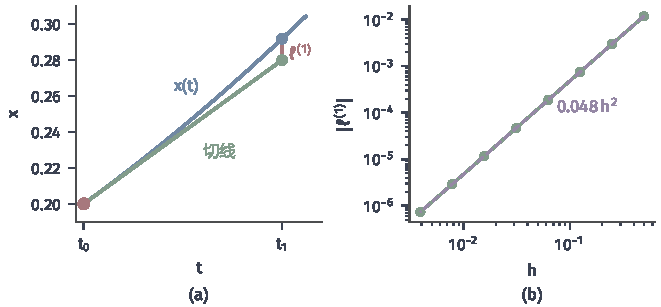
\includegraphics[width=112mm]{figures/06-differential-equations/01-ordinary-differential-equations/matplotlib/odenum-euler-one-step/figure.pdf}
 \caption{显式Euler方法的第一步。(a)$h=1/2$：蓝线是真解，绿线是起点处的切线，红色线段是局部截断误差$\ell^{(1)}$。(b)绿点是不同步长下的$\lvert\ell^{(1)}\rvert$，紫色虚线是主要部分$0.048h^2$。}
 \label{fig:odenum-euler-one-step}
\end{BookInlineFigure}

\begin{definition}[方法的阶]
 \label{def:odenum-order}
 设一步方法的局部截断误差沿真解满足：存在与$k$、$h$无关的$C$和$h_0>0$，使当$0<h\leq h_0$时，对所有$k$有
 \begin{equation}
  \bigl\lVert\bm{\ell}^{(k+1)}\bigr\rVert_2\leq Ch^{p+1},
  \label{eq:odenum-order}
 \end{equation}
 就称方法在这个问题上具有\term{局部误差阶}（local order）$p+1$，称$p$为\term{方法的阶}（order of a method）。
\end{definition}

由式~\eqref{eq:odenum-euler-local-bound}，当$\bm{x}\in C^2$时显式Euler方法的阶为$1$。一步误差$h^2$，方法的阶却是$1$，原因是走完$T$要$N=T/h$步，$N\cdot h^2$恰好是$Th$。这个数步数的算术还不是证明，第~\ref{sec:odenum-error-convergence}节将补全它需要的条件。

\paragraph{步长细化的比较}
一个基本的检验是把步长不断减半，看终点误差怎样变化。表~\ref{tab:odenum-euler-refine}列出例~\eqref{eq:odenum-running}的结果。显式Euler方法每步求值一次右端，所以$N$同时就是计算量。

\begin{BookInlineTable}
 \centering
 \caption{显式Euler方法的步长细化。问题为式~\eqref{eq:odenum-running}，误差指$x^{(N)}-x(1)$，比值是上一行误差除以本行误差。}
 \label{tab:odenum-euler-refine}
 \begin{tabular}{rrrrr}
  \toprule
  $N$ & $h$ & $x^{(N)}$ & 误差 & 比值\\
  \midrule
  2 & 0.5 & 0.380800 & $-2.381\times10^{-2}$ & \\
  4 & 0.25 & 0.392434 & $-1.218\times10^{-2}$ & 1.95\\
  8 & 0.125 & 0.398476 & $-6.134\times10^{-3}$ & 1.99\\
  16 & 0.0625 & 0.401535 & $-3.075\times10^{-3}$ & 1.99\\
  32 & 0.03125 & 0.403071 & $-1.539\times10^{-3}$ & 2.00\\
  \bottomrule
 \end{tabular}
\end{BookInlineTable}

比值趋于$2$：计算量加倍，误差只减半。把误差写成$0.0493/N$（图~\ref{fig:odenum-euler-refinement}），可知要把误差压到$10^{-6}$，约需$5\times10^{4}$次右端求值。对这样一个简单方程，这个价钱是昂贵的，它也给后面的高阶方法提供了比较的基准。

\begin{BookInlineFigure}
 \centering
 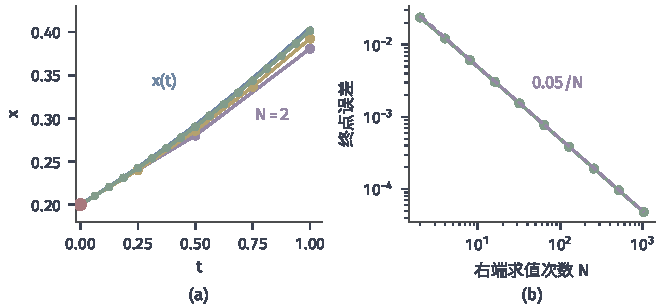
\includegraphics[width=112mm]{figures/06-differential-equations/01-ordinary-differential-equations/matplotlib/odenum-euler-refinement/figure.pdf}
 \caption{显式Euler方法的步长细化。(a)蓝线是真解，紫、黄、绿折线分别是$N=2,4,16$的数值解。(b)$t=1$处的误差随右端求值次数$N$的变化，紫色虚线是参考直线$0.05/N$。}
 \label{fig:odenum-euler-refinement}
\end{BookInlineFigure}


\section{Runge--Kutta方法}
\label{sec:odenum-runge-kutta}

Euler方法整步只用起点的斜率，弯曲的解曲线被它的切线代替。要想更准，自然想到在这一步内部多看几次斜率，再把它们组合起来。看哪几处、怎样组合，才能真正提高阶数？

\paragraph{主要思想：匹配Taylor展开}
先看真解一步走到哪里。设$\bm{f}$二次连续可微，记
\begin{equation}
 \bm{g}=\partial_t\bm{f}+\partial_{\bm{x}}\bm{f}\,\bm{f},
 \label{eq:odenum-total-derivative}
\end{equation}
它是$\bm{f}$沿解的全导数，也就是$\ddot{\bm{x}}$。解的Taylor展开为
\[
 \bm{x}(t+h)=\bm{x}+h\bm{f}+\frac{h^2}{2}\bm{g}+O(h^3),
\]
右端各量在$(t,\bm{x}(t))$处取值。Euler方法只匹配了前两项，$h^2$一项就是它的局部误差。

现在允许多读一次斜率。先取起点斜率，再沿它试探着走到$t+\alpha h$，在那里读第二个斜率：
\[
 \bm{k}_1=\bm{f}(t,\bm{x}),\qquad
 \bm{k}_2=\bm{f}\bigl(t+\alpha h,\bm{x}+\alpha h\bm{k}_1\bigr).
\]
最后用两个斜率的加权平均前进：
\[
 \bm{\Psi}_h(t,\bm{x})=\bm{x}+h\bigl(b_1\bm{k}_1+b_2\bm{k}_2\bigr).
\]

$\alpha,b_1,b_2$待定。把$\bm{k}_2$在$(t,\bm{x})$处作Taylor展开，$h$的一次项正好由式~\eqref{eq:odenum-total-derivative}的全导数给出：
\[
 \bm{k}_2=\bm{f}+\alpha h\,\bm{g}+O(h^2).
\]
代入更新式，得到
\[
 \bm{\Psi}_h(t,\bm{x})=\bm{x}+(b_1+b_2)h\bm{f}+\alpha b_2h^2\bm{g}+O(h^3).
\]

与真解的展开逐项比较，要让$h$和$h^2$的系数都对上，需要
\begin{equation}
 b_1+b_2=1,\qquad \alpha b_2=\frac{1}{2}.
 \label{eq:odenum-two-stage-conditions}
\end{equation}
三个未知数、两个方程，于是有一族二阶方法。取$\alpha=1/2$，$b_1=0$，$b_2=1$，得到\term{中点方法}（midpoint method）：
\begin{equation}
 \begin{aligned}
  \bm{k}_1&=\bm{f}\bigl(t_k,\bm{x}^{(k)}\bigr),\\
  \bm{k}_2&=\bm{f}\Bigl(t_k+\frac{h}{2},\ \bm{x}^{(k)}+\frac{h}{2}\bm{k}_1\Bigr),\\
  \bm{x}^{(k+1)}&=\bm{x}^{(k)}+h\bm{k}_2.
 \end{aligned}
 \label{eq:odenum-midpoint}
\end{equation}
另一个选择$\alpha=1$，$b_1=b_2=1/2$是Heun方法，它在第~\ref{sec:odenum-adaptive}节还要用到。

中点方法的几何含义很清楚（图~\ref{fig:odenum-midpoint-steps}）：积分$\int\bm{f}\,\mathrm{d}s$用区间中点的值乘$h$来近似，这是中点求积公式。困难在于中点处的状态未知，于是先用起点斜率走半步来试探它。试探点本身只有一阶精度，但$\bm{f}$在那里的值只需准到$O(h^2)$，一乘$h$就足够了。

\begin{BookInlineFigure}
 \centering
 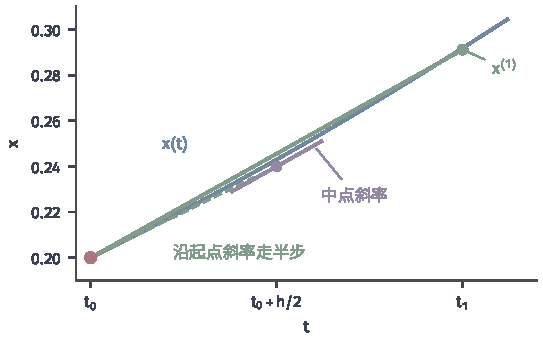
\includegraphics[width=92mm]{figures/06-differential-equations/01-ordinary-differential-equations/matplotlib/odenum-midpoint-steps/figure.pdf}
 \caption{中点方法的第一步，$h=1/2$，问题为式~\eqref{eq:odenum-running}。蓝线是真解，绿色虚线沿起点斜率走半步到紫点，紫色短线是在紫点读到的斜率$k_2$，绿色实线从红色初值出发，沿斜率$k_2$走满一步到$x^{(1)}$。}
 \label{fig:odenum-midpoint-steps}
\end{BookInlineFigure}

中点方法的手算只需把式~\eqref{eq:odenum-midpoint}代入两轮。对例~\eqref{eq:odenum-running}取$h=0.5$，第一轮的结果为
\[
 k_1=0.16,\qquad 0.2+0.25k_1=0.24,\qquad k_2=0.24\times0.76=0.1824,
\]
于是
\[
 x^{(1)}=0.2+0.5\times0.1824=0.2912.
\]
第二轮从$x^{(1)}$出发，同样得到
\[
 k_1=0.206403,\qquad 0.342801,\qquad k_2=0.225288,
\]
所以$x^{(2)}=0.403844$，终点误差约$-7.7\times10^{-4}$，比Euler方法的$-0.0238$小了约三十倍，而右端求值次数只从$2$增加到$4$。

\paragraph{主要思想：多级与经典四阶方法}
上面的做法可以一般化。$s$级\term{显式Runge--Kutta方法}（explicit Runge--Kutta method）依次计算$s$个\term{阶段斜率}（stage slope）：
\begin{equation}
 \bm{k}_i=\bm{f}\Bigl(t_k+c_ih,\ \bm{x}^{(k)}+h\sum_{j<i}a_{i,j}\bm{k}_j\Bigr),\quad i=1,\ldots,s,
 \label{eq:odenum-rk-stages}
\end{equation}
再组合成一步更新：
\begin{equation}
 \bm{x}^{(k+1)}=\bm{x}^{(k)}+h\sum_{i=1}^{s}b_i\bm{k}_i.
 \label{eq:odenum-rk-update}
\end{equation}
每个$\bm{k}_i$只用前面已算出的斜率，所以依次代入即可，这就是“显式”的含义。系数由匹配Taylor展开决定，中点方法是$s=2$的情形。

阶数越高，要匹配的项越多。沿解的高阶全导数含有$\bm{f}$的各阶偏导的多种组合，四阶需要同时满足八个代数条件。最著名的解是\term{经典四阶Runge--Kutta方法}（classical fourth-order Runge--Kutta method），简称RK4：
\begin{equation}
 \begin{aligned}
  \bm{k}_1&=\bm{f}\bigl(t_k,\bm{x}^{(k)}\bigr),\\
  \bm{k}_2&=\bm{f}\Bigl(t_k+\frac{h}{2},\ \bm{x}^{(k)}+\frac{h}{2}\bm{k}_1\Bigr),\\
  \bm{k}_3&=\bm{f}\Bigl(t_k+\frac{h}{2},\ \bm{x}^{(k)}+\frac{h}{2}\bm{k}_2\Bigr),\\
  \bm{k}_4&=\bm{f}\bigl(t_k+h,\ \bm{x}^{(k)}+h\bm{k}_3\bigr),\\
  \bm{x}^{(k+1)}&=\bm{x}^{(k)}+\frac{h}{6}\bigl(\bm{k}_1+2\bm{k}_2+2\bm{k}_3+\bm{k}_4\bigr).
 \end{aligned}
 \label{eq:odenum-rk4}
\end{equation}

权重$1,2,2,1$有一个可以直接验证的来源。若$\bm{f}$不依赖状态，四个斜率分别是$\bm{f}(t_k)$、$\bm{f}(t_k+h/2)$、$\bm{f}(t_k+h/2)$、$\bm{f}(t_k+h)$，更新式化为
\[
 \bm{x}^{(k+1)}-\bm{x}^{(k)}=\frac{h}{6}\Bigl(\bm{f}(t_k)+4\bm{f}\bigl(t_k+\tfrac{h}{2}\bigr)+\bm{f}(t_k+h)\Bigr),
\]
正是Simpson求积公式。中点权重$4$被拆给了两个中点估计$\bm{k}_2$和$\bm{k}_3$，它们从不同的试探点读取斜率，彼此修正。

\begin{theorem}[RK4的阶]
 \label{thm:odenum-rk4-order}
 设$\bm{f}$在包含解曲线的开集上四次连续可微，$\bm{x}(t)$是$[t_0,t_0+T]$上的解。则存在$C,h_0>0$，使当$0<h\leq h_0$时，RK4的局部截断误差满足
 \begin{equation}
  \bigl\lVert\bm{\ell}^{(k+1)}\bigr\rVert_2\leq Ch^{5}.
  \label{eq:odenum-rk4-local}
 \end{equation}
\end{theorem}

这个结论的证明需要把真解和数值更新都展开到$h^4$，逐项核对八个代数条件，篇幅较长，读者可查阅\scite{math-hairer1993ode}。定理的条件不能省：光滑性决定了展开能够进行到第几项，下文的例子会说明它不成立时阶数怎样丢失。

\paragraph{计算过程}
RK4每一步按式~\eqref{eq:odenum-rk4}依次算四个斜率。下面仍用例~\eqref{eq:odenum-running}的数据手算，取$h=0.5$，$N=2$。

\needspace{6\baselineskip}
\paragraph{变量}
\begin{itemize}
 \item $\bm{x}^{(k)}\in\mathbb{R}^{n}$：第$k$个网格点的数值解。
 \item $\bm{k}_1,\bm{k}_2,\bm{k}_3,\bm{k}_4\in\mathbb{R}^{n}$：本步的四个阶段斜率，用完即弃。
 \item $\bm{y}_2,\bm{y}_3,\bm{y}_4\in\mathbb{R}^{n}$：读取后三个斜率的试探状态。
\end{itemize}

\paragraph{初始化}
与Euler方法相同，把数值解初始化为初值。例中
\[
 x^{(0)}=0.2,\qquad t_0=0,\qquad h=0.5,\qquad N=2.
\]

\needspace{6\baselineskip}
\paragraph{每轮更新}
对$k=0,1,\ldots,N-1$依次执行：
\begin{enumerate}

 \item \textbf{起点斜率。}计算$\bm{k}_1=\bm{f}(t_k,\bm{x}^{(k)})$。例中第一轮
 \[
  k_1=0.2\times0.8=0.16.
 \]

 \item \textbf{第一次试探中点。}令
 \[
  \bm{y}_2=\bm{x}^{(k)}+\frac{h}{2}\bm{k}_1,\qquad \bm{k}_2=\bm{f}\bigl(t_k+\tfrac{h}{2},\bm{y}_2\bigr).
 \]
 例中第一轮
 \[
  y_2=0.24,\qquad k_2=0.24\times0.76=0.1824.
 \]

 \item \textbf{第二次试探中点。}令
 \[
  \bm{y}_3=\bm{x}^{(k)}+\frac{h}{2}\bm{k}_2,\qquad \bm{k}_3=\bm{f}\bigl(t_k+\tfrac{h}{2},\bm{y}_3\bigr).
 \]
 例中第一轮
 \[
  y_3=0.2456,\qquad k_3=0.2456\times0.7544=0.185281.
 \]

 \item \textbf{试探终点。}令
 \[
  \bm{y}_4=\bm{x}^{(k)}+h\bm{k}_3,\qquad \bm{k}_4=\bm{f}\bigl(t_k+h,\bm{y}_4\bigr).
 \]
 例中第一轮
 \[
  y_4=0.292640,\qquad k_4=0.207002.
 \]

 \item \textbf{加权前进。}由式~\eqref{eq:odenum-rk4}的最后一行计算$\bm{x}^{(k+1)}$。例中第一轮
 \[
  x^{(1)}=0.2+\frac{0.5}{6}\times1.102363=0.2918636.
 \]
 例中第二轮从$x^{(1)}$出发，依次得到
 \[
  \begin{gathered}
   k_1=0.206679,\quad y_2=0.343533,\quad k_2=0.225518,\\
   y_3=0.348243,\quad k_3=0.226970,\\
   y_4=0.405349,\quad k_4=0.241041,
  \end{gathered}
 \]
 于是
 \[
  x^{(2)}=0.2918636+\frac{0.5}{6}\times1.352696=0.4045883.
 \]

 \item \textbf{停止。}当$k+1=N$时结束。例中$k+1=2$，退出循环。
\end{enumerate}
最终例中得到$x^{(2)}=0.404588$，真值为$0.404610$，误差约$-2.1\times10^{-5}$，只用了$8$次右端求值。图~\ref{fig:odenum-rk4-stages}标出第一步的四个采样位置。

\begin{BookInlineFigure}
 \centering
 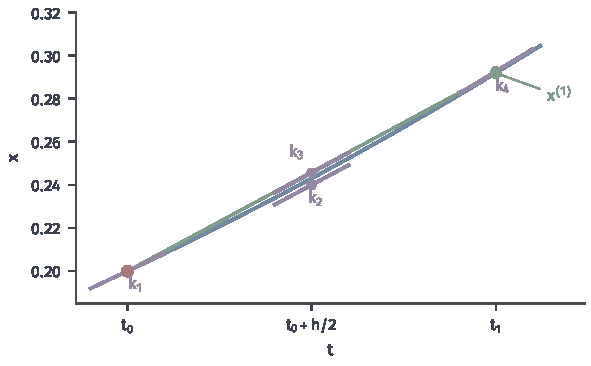
\includegraphics[width=100mm]{figures/06-differential-equations/01-ordinary-differential-equations/matplotlib/odenum-rk4-stages/figure.pdf}
 \caption{RK4的第一步，$h=1/2$，问题为式~\eqref{eq:odenum-running}。紫点是四个采样位置$(t_0,x_0)$、$(t_0+h/2,y_2)$、$(t_0+h/2,y_3)$、$(t_1,y_4)$，紫色短线是读到的四个斜率；绿线从红色初值走到$x^{(1)}$，蓝线是真解。}
 \label{fig:odenum-rk4-stages}
\end{BookInlineFigure}

\paragraph{光滑性决定阶数能否兑现}
定理~\ref{thm:odenum-rk4-order}要求右端足够光滑。把例~\eqref{eq:odenum-running}改成带时间跳变的方程：
\[
 \dot{x}=r(t)x(1-x),\qquad
 r(t)=\begin{cases}1,&t<t_{*},\\2,&t\geq t_{*},\end{cases}
\]
其中$t_{*}=1/\sqrt{2}$，闭式解用$\int_0^tr$代替$t$仍然成立。图~\ref{fig:odenum-rk4-jump}的红线是均匀网格上RK4的终点误差。$t_{*}$落在某一步内部，四个采样点无法判断跳变发生在这一步的什么位置，这一步的局部误差只有$O(h)$，一步就把全局误差拖到一阶，并随$t_{*}$在步内的相对位置起伏。

\begin{BookInlineFigure}
 \centering
 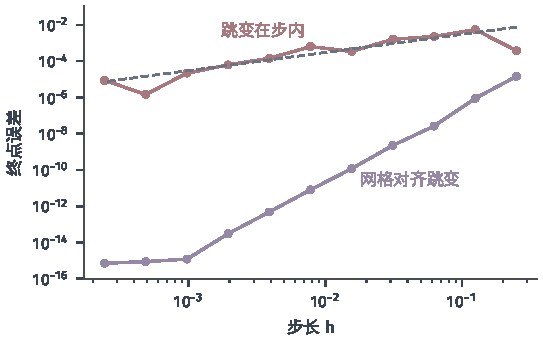
\includegraphics[width=92mm]{figures/06-differential-equations/01-ordinary-differential-equations/matplotlib/odenum-rk4-jump/figure.pdf}
 \caption{右端带跳变时RK4的终点误差。红线：均匀网格，跳变点$t_{*}=1/\sqrt{2}$落在步内；灰色虚线是参考直线$0.03h$。紫线：把$t_{*}$放在网格点上，两侧分别用均匀步长积分，四阶恢复，直到舍入误差使曲线变平。}
 \label{fig:odenum-rk4-jump}
\end{BookInlineFigure}

补救办法也在图中。若已知跳变时刻，把它放到网格点上，在两侧分别积分（紫线），每段内部$\bm{f}$都是光滑的，阶数恢复为四。

\paragraph{每步成本与总成本}
高阶方法每步更贵，比较时必须看走完全程的总求值次数。图~\ref{fig:odenum-rk-convergence}左图的三条直线斜率分别为$1$、$2$、$4$，与三个方法的阶一致。右图把横轴换成右端求值次数，表~\ref{tab:odenum-cost}给出达到同一精度的成本。

\begin{BookInlineFigure}
 \centering
 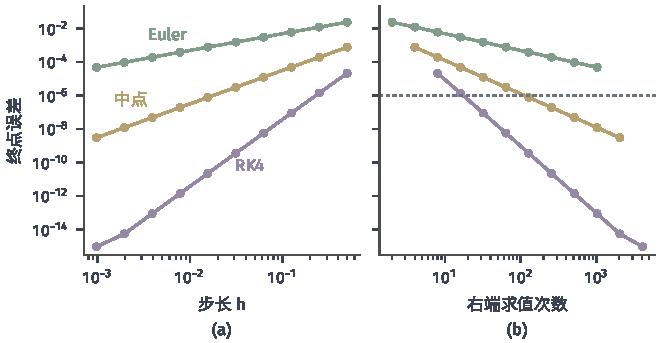
\includegraphics[width=112mm]{figures/06-differential-equations/01-ordinary-differential-equations/matplotlib/odenum-rk-convergence/figure.pdf}
 \caption{三种方法在式~\eqref{eq:odenum-running}上$t=1$处的误差。绿、黄、紫线分别是Euler、中点、RK4。(a)误差对步长；(b)误差对右端求值次数，灰色虚线是$10^{-6}$。RK4在$h$很小时误差碰到舍入水平。}
 \label{fig:odenum-rk-convergence}
\end{BookInlineFigure}

\begin{BookInlineTable}
 \centering
 \caption{式~\eqref{eq:odenum-running}上使$t=1$处误差不超过给定精度所需的右端求值次数（步数以约$3\%$递增搜索，故为近似值）。}
 \label{tab:odenum-cost}
 \begin{tabular}{rrrr}
  \toprule
  目标精度 & Euler（每步1次） & 中点（每步2次） & RK4（每步4次）\\
  \midrule
  $10^{-2}$ & 5 & 2 & 4\\
  $10^{-4}$ & $5.0\times10^{2}$ & 12 & 8\\
  $10^{-6}$ & $4.9\times10^{4}$ & $1.2\times10^{2}$ & 20\\
  $10^{-8}$ & $5.0\times10^{6}$ & $1.1\times10^{3}$ & 56\\
  \bottomrule
 \end{tabular}
\end{BookInlineTable}

表中的规律是：精度要求越高，高阶方法的优势越大；要求只有$10^{-2}$时，三者的成本差不多，RK4反而比中点方法多花一倍。这个比较只在解足够光滑时有意义，图~\ref{fig:odenum-rk4-jump}的情形下RK4多花的求值次数并不能换来四阶精度。



\section{误差与收敛}
\label{sec:odenum-error-convergence}

前两节看到的现象是：一步误差为$h^{p+1}$时，终点误差表现为$h^{p}$。数步数的算术说明不了这件事，因为早期产生的误差还要被后面的每一步继续传播，可能被放大。什么条件下这种累积可控？

\paragraph{一步局部误差的约定}
先把量纲说清楚。本书的局部截断误差~\eqref{eq:odenum-local-error}没有除以步长，它是一步之内产生的偏差，单位与状态相同。若方法的阶为$p$，它的大小是$O(h^{p+1})$。

有些文献把$\bm{\ell}^{(k+1)}/h$称为截断误差，这时阶为$p$的方法“局部截断误差”写作$O(h^{p})$。两种写法描述同一件事，读其他资料时要先确认定义。下表对比本章会用到的两个量。

\begin{BookInlineTable}
 \centering
 \caption{局部截断误差与全局误差的对比（阶为$p$的方法）。}
 \label{tab:odenum-local-global}
 \begin{tabular}{lll}
  \toprule
  & 局部截断误差$\bm{\ell}^{(k+1)}$ & 全局误差$\bm{e}^{(k)}$\\
  \midrule
  出发点 & 真解点$\bm{x}(t_k)$ & 实际算出的序列\\
  包含 & 一步更新的缺陷 & 全部历史的累积\\
  大小 & $O(h^{p+1})$ & 条件满足时$O(h^{p})$\\
  能否实际算出 & 需要真解 & 需要真解\\
  \bottomrule
 \end{tabular}
\end{BookInlineTable}

\paragraph{误差的传播图景}
式~\eqref{eq:odenum-error-split}说明每步的新误差与旧误差叠加。还可以换一个角度看：每步产生的偏差会被此后的真实流映射搬运到终点。把$\bm{\varphi}_{t,t_N}$作用于网格值，相邻两项之差就是第$k$步的贡献，它们相加后中间项全部抵消，在没有初值误差时得到
\begin{equation}
 \bm{e}^{(N)}=\sum_{k=0}^{N-1}\Bigl[\bm{\varphi}_{t_{k+1},t_N}\bigl(\bm{x}^{(k+1)}\bigr)-\bm{\varphi}_{t_k,t_N}\bigl(\bm{x}^{(k)}\bigr)\Bigr].
 \label{eq:odenum-telescoping}
\end{equation}

图~\ref{fig:odenum-error-fan}左侧画出这个分解。绿色折线是Euler网格值与真解之差，每个绿点处长出一条黄线，它是从该点出发的真解。相邻黄线在终点的间距，正是式~\eqref{eq:odenum-telescoping}的一项。

\begin{BookInlineFigure}
 \centering
 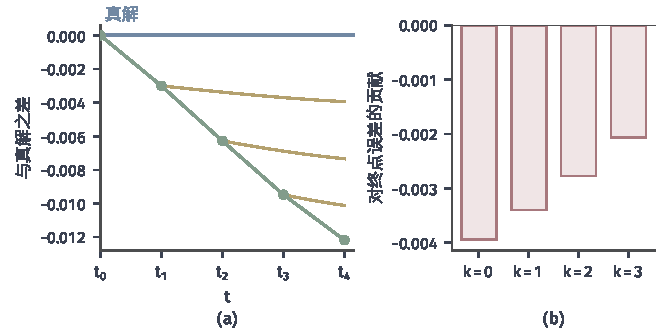
\includegraphics[width=112mm]{figures/06-differential-equations/01-ordinary-differential-equations/matplotlib/odenum-error-fan/figure.pdf}
 \caption{显式Euler方法的误差累积，问题为式~\eqref{eq:odenum-running}，$h=1/4$。(a)纵轴是与真解之差：蓝线是真解，绿线是网格值，黄线是从各网格值出发的真解。(b)式~\eqref{eq:odenum-telescoping}的四项，即每步偏差被搬运到$t=1$时的大小，四项之和等于终点误差$-0.01218$。}
 \label{fig:odenum-error-fan}
\end{BookInlineFigure}

例中四项依次为$-0.00394$、$-0.00340$、$-0.00277$、$-0.00206$，第一步的贡献最大。第一步本身的局部误差只有$-0.00300$，搬运到终点后变成$-0.00394$，因为这里$\partial_xf=1-2x>0$，邻近的解随时间分开。流映射放大扰动的程度决定了累积的结果，这与第~\ref{chap:ode-sensitivity}章的结论是同一回事。

\paragraph{一步稳定性}
要给出误差界，需要一个条件控制式~\eqref{eq:odenum-error-split}的第一项。连续情形的对应结论是Gronwall估计：若$\bm{f}$关于状态满足Lipschitz条件，常数为$L$，则从两个初值出发的解之差至多按$\mathrm{e}^{L(t-s)}$增长，推导见第~\ref{chap:ode-sensitivity}章。离散情形要求的是这种增长的一步版本。

数值解只需要在真解附近受控。取半径$\rho>0$，记真解周围的管状区域为
\begin{equation}
 \bm{K}_{\rho}=\bigl\{(t,\bm{y}):t\in[t_0,t_0+T],\ \lVert\bm{y}-\bm{x}(t)\rVert_2\leq\rho\bigr\}.
 \label{eq:odenum-tube}
\end{equation}

\begin{definition}[一步稳定性]
 \label{def:odenum-one-step-stability}
 设存在$\Lambda>0$和$h_0>0$，使当$0<h\leq h_0$时，对$\bm{K}_{\rho}$中所有同一时刻$t$的点$(t,\bm{y})$与$(t,\bm{z})$都有
 \begin{equation}
  \bigl\lVert\bm{\Psi}_h(t,\bm{y})-\bm{\Psi}_h(t,\bm{z})\bigr\rVert_2\leq(1+h\Lambda)\lVert\bm{y}-\bm{z}\rVert_2,
  \label{eq:odenum-one-step-stability}
 \end{equation}
 就称一步方法在$\bm{K}_{\rho}$上具有\term{一步稳定性}（one-step stability）。
\end{definition}

式中放大因子写成$1+h\Lambda$有明确的用意。走$N=T/h$步，累积因子至多是$(1+h\Lambda)^{T/h}\leq\mathrm{e}^{\Lambda T}$，不随$h\to0$增大。如果放大因子只是$1+\sqrt{h}$，下文会看到累积因子将趋于无穷。

这个条件可以逐个方法验证。设$\bm{f}$关于状态的Lipschitz常数在所考虑的区域上为$L$。显式Euler方法两点的差是
\[
 \bigl\lVert\bm{\Psi}_h(t,\bm{y})-\bm{\Psi}_h(t,\bm{z})\bigr\rVert_2
 \leq\lVert\bm{y}-\bm{z}\rVert_2+h\bigl\lVert\bm{f}(t,\bm{y})-\bm{f}(t,\bm{z})\bigr\rVert_2,
\]
第二项不超过$hL\lVert\bm{y}-\bm{z}\rVert_2$，所以$\Lambda=L$。

中点方法要多一层试探点。设$\bm{f}$在更大的管$\bm{K}_{2\rho}$上有界、Lipschitz常数为$L$，$h_0$足够小，使试探点仍在$\bm{K}_{2\rho}$内。两个点的第一个斜率之差不超过$L\lVert\bm{y}-\bm{z}\rVert_2$，第二个斜率之差满足
\[
 \lVert\bm{k}_2-\bm{k}_2'\rVert_2\leq L\Bigl(1+\frac{hL}{2}\Bigr)\lVert\bm{y}-\bm{z}\rVert_2.
\]
于是中点方法满足式~\eqref{eq:odenum-one-step-stability}，常数为
\[
 \Lambda=L\Bigl(1+\frac{h_0L}{2}\Bigr).
\]

一般的显式Runge--Kutta方法做法相同。由式~\eqref{eq:odenum-rk-stages}逐级得到
\[
 \lVert\bm{k}_i-\bm{k}_i'\rVert_2\leq L\Bigl(\lVert\bm{y}-\bm{z}\rVert_2+h\sum_{j<i}\lvert a_{i,j}\rvert\,\lVert\bm{k}_j-\bm{k}_j'\rVert_2\Bigr),
\]
级数有限，归纳即可得到形如式~\eqref{eq:odenum-one-step-stability}的估计，$\Lambda$由$L$、系数和$h_0$决定。

\paragraph{离散Gronwall不等式}
把一步稳定性代入式~\eqref{eq:odenum-error-split}，会得到一个数列的递推不等式。下面的引理把这种递推解开，它是连续Gronwall估计的离散版本。

\begin{lemma}[离散Gronwall不等式]
 \label{lem:odenum-discrete-gronwall}
 设$q>0$，$b\geq0$，非负数列满足$a_{j+1}\leq(1+q)a_j+b$，$j=0,\ldots,m-1$。则对$j=0,\ldots,m$，
 \begin{equation}
  a_j\leq(1+q)^{j}a_0+\frac{(1+q)^{j}-1}{q}\,b.
  \label{eq:odenum-discrete-gronwall}
 \end{equation}
\end{lemma}

\begin{proof}
 对$j$作归纳。$j=0$时不等式两边都是$a_0$。

 设式~\eqref{eq:odenum-discrete-gronwall}对$j$成立，把它代入$a_{j+1}\leq(1+q)a_j+b$，得到
 \[
  a_{j+1}\leq(1+q)^{j+1}a_0+\Bigl[(1+q)\frac{(1+q)^{j}-1}{q}+1\Bigr]b.
 \]
 通分后方括号内的量化简为
 \[
  \frac{(1+q)^{j+1}-(1+q)+q}{q}=\frac{(1+q)^{j+1}-1}{q},
 \]
 这正是$j+1$时的结论。
\end{proof}

\paragraph{全局误差定理}
现在把三种误差放到一起。

\begin{theorem}[有限区间上的全局误差界]
 \label{thm:odenum-global-error}
 设$\bm{x}(t)$是式~\eqref{eq:odenum-ivp}在$[t_0,t_0+T]$上的解，一步方法在$\bm{K}_{\rho}$上满足一步稳定性~\eqref{eq:odenum-one-step-stability}，并且对$0<h\leq h_0$与所有$k$，
 \begin{equation}
  \bigl\lVert\bm{\ell}^{(k+1)}\bigr\rVert_2\leq Ch^{p+1},\quad
  \bigl\lVert\bm{\delta}^{(0)}\bigr\rVert_2\leq\varepsilon_0,\quad
  \bigl\lVert\bm{\delta}^{(k+1)}\bigr\rVert_2\leq\varepsilon.
  \label{eq:odenum-global-hypotheses}
 \end{equation}
 记
 \begin{equation}
  E(h)=\mathrm{e}^{\Lambda T}\varepsilon_0+\frac{\mathrm{e}^{\Lambda T}-1}{\Lambda}\Bigl(Ch^{p}+\frac{\varepsilon}{h}\Bigr).
  \label{eq:odenum-global-bound-def}
 \end{equation}
 若$h\leq h_0$且$E(h)\leq\rho$，则式~\eqref{eq:odenum-computed}的序列都留在管内，并且对$k=0,1,\ldots,N$，
 \begin{equation}
  \bigl\lVert\bm{e}^{(k)}\bigr\rVert_2\leq\mathrm{e}^{\Lambda kh}\varepsilon_0+\frac{\mathrm{e}^{\Lambda kh}-1}{\Lambda}\Bigl(Ch^{p}+\frac{\varepsilon}{h}\Bigr)\leq E(h).
  \label{eq:odenum-global-bound}
 \end{equation}
\end{theorem}

\begin{proof}
 记$a_k=\lVert\bm{e}^{(k)}\rVert_2$，$q=h\Lambda$，$b=Ch^{p+1}+\varepsilon$。对$k$归纳证明式~\eqref{eq:odenum-global-bound}，同时得到$(t_k,\bm{x}^{(k)})\in\bm{K}_{\rho}$。

 $k=0$时$a_0\leq\varepsilon_0\leq E(h)\leq\rho$。

 设直到$k$结论都成立，那么$\bm{x}^{(k)}$与$\bm{x}(t_k)$都在管内，可以对式~\eqref{eq:odenum-error-split}用一步稳定性和假设~\eqref{eq:odenum-global-hypotheses}，得到
 \[
  a_{j+1}\leq(1+q)a_j+b,\qquad j=0,\ldots,k.
 \]
 由引理~\ref{lem:odenum-discrete-gronwall}，
 \[
  a_{k+1}\leq(1+q)^{k+1}a_0+\frac{(1+q)^{k+1}-1}{q}\,b.
 \]

 用$1+q\leq\mathrm{e}^{q}$，且$q=h\Lambda$，第一项不超过$\mathrm{e}^{\Lambda(k+1)h}\varepsilon_0$。第二项的系数满足
 \[
  \frac{(1+q)^{k+1}-1}{q}\,b\leq\frac{\mathrm{e}^{\Lambda(k+1)h}-1}{h\Lambda}\,b.
 \]
 其中$b/h=Ch^{p}+\varepsilon/h$，所以式~\eqref{eq:odenum-global-bound}对$k+1$成立。

 因为$(k+1)h\leq T$，右端不超过$E(h)\leq\rho$，$\bm{x}^{(k+1)}$仍在管内，归纳完成。
\end{proof}

式~\eqref{eq:odenum-global-bound}的三项对应三种误差。初值误差被放大$\mathrm{e}^{\Lambda T}$倍。截断误差每步$Ch^{p+1}$，共$T/h$步，累积成$Ch^{p}$的量级，常数$(\mathrm{e}^{\Lambda T}-1)/\Lambda$扮演放大因子。计算误差同样累积，但少除了一次$h$，留下$\varepsilon/h$。

\paragraph{算例：误差界与实际误差}
\begin{example}[Euler方法的误差界]
 \label{ex:odenum-euler-bound}
 对例~\eqref{eq:odenum-running}用显式Euler方法，并设计算无误差。

 取$\rho=0.1$。真解在$[0,1]$上取值于$[0.2,0.4047]$，所以管内状态落在$[0.1,0.505]$中，在这里
 \[
  \lvert\partial_xf\rvert=\lvert1-2x\rvert\leq0.8,
 \]
 可取$\Lambda=L=0.8$。

 由$\ddot{x}=(1-2x)x(1-x)$，它在$[0.2,0.4047]$上的最大值约为$0.0962$，在$x\approx0.2113$处取得。由式~\eqref{eq:odenum-euler-local-bound}可取
 \[
  C=\frac{0.0962}{2}=0.0481,\qquad p=1.
 \]

 代入式~\eqref{eq:odenum-global-bound-def}，$\varepsilon_0=\varepsilon=0$，得到
 \[
  E(h)=\frac{\mathrm{e}^{0.8}-1}{0.8}\times0.0481\,h\approx0.0737\,h.
 \]
 $h=0.5$时$E(h)\approx0.0368$，满足$E(h)\leq\rho$，实际误差$0.0238$在这个界内。当$h\to0$时实际误差约为$0.0493h$，界比它大约百分之五十。
\end{example}

\paragraph{一步误差的阶何时给出全局误差的阶}
定理~\ref{thm:odenum-global-error}给出了答案。取$\varepsilon_0=O(h^{p})$，$\varepsilon=O(h^{p+1})$，又要$\bm{\ell}^{(k+1)}=O(h^{p+1})$在所有步上一致成立，方法一步稳定，并且真解在整个区间存在，那么全局误差就是$O(h^{p})$。下面逐条看去掉条件会怎样。

\emph{没有一步稳定性。}考虑$\dot{x}=0$，$x(0)=0$，真解恒为零，取映射
\[
 \Psi_h(y)=(1+\sqrt{h})\,y.
\]
沿真解$\Psi_h(0)=0$，局部截断误差严格为零。可是放大因子是$1+\sqrt{h}$，不是$1+O(h)$。给初值一个$h^2$的扰动，走到$T=1$后得到
\[
 \lvert x^{(N)}\rvert=(1+\sqrt{h})^{1/h}h^{2}.
\]
$h=0.01$时它约等于$1.38$，并且$h\to0$时趋于无穷。局部误差再小也不能保证收敛。

\emph{局部误差只在部分步上达到高阶。}图~\ref{fig:odenum-rk4-jump}就是这种情形：跳变所在的那一步局部误差只有$O(h)$，其余各步是$O(h^{5})$，全局误差被那一步决定，退回一阶。

\emph{初值误差和计算误差不随步长减小。}固定的$\varepsilon_0$只给出误差的下限。更值得注意的是计算误差项$\varepsilon/h$：它随$h$减小而增大，于是全局误差关于步长是一个先降后升的曲线。对$Ch^{p}+\varepsilon/h$求最小，当$p=1$时
\[
 h_{*}=\sqrt{\frac{\varepsilon}{C}},
\]
此时最小值为$2\sqrt{C\varepsilon}$。图~\ref{fig:odenum-roundoff-v}把Euler方法每步的结果舍入到小数点后六位，亲手制造了这个现象。

\begin{BookInlineFigure}
 \centering
 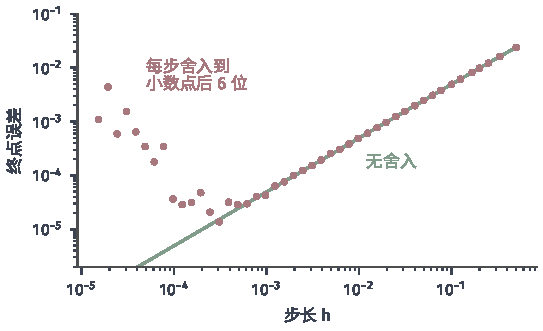
\includegraphics[width=92mm]{figures/06-differential-equations/01-ordinary-differential-equations/matplotlib/odenum-roundoff-v/figure.pdf}
 \caption{显式Euler方法的截断误差与舍入误差，问题为式~\eqref{eq:odenum-running}，$T=1$。绿线不作舍入，红点是每步把结果舍入到小数点后六位时的终点误差。$h$太大时截断误差主导，$h$太小时舍入误差累积主导。}
 \label{fig:odenum-roundoff-v}
\end{BookInlineFigure}

图中误差的最小值约为$10^{-5}$，出现在$h\approx3\times10^{-4}$附近，再缩小步长，误差反而变大。这比最坏情形的界算出的$h_{*}$更小，因为实际舍入有正有负、部分抵消，定理~\ref{thm:odenum-global-error}只给出上界。

\emph{真解在区间上不存在。}对$\dot{x}=x^2$，$x(0)=1$，解在$t=1$爆炸，定理的条件不成立。Euler方法却照常输出，取$h=0.5$走到$t=2$：
\[
 1,\quad 1.5,\quad 2.625,\quad 6.070,\quad 24.495.
\]
数值方法给出有限的数字，并不说明解在那里存在，第~\ref{chap:ode-existence-continuation}章的延拓判据不能省。


\section{刚性问题}
\label{sec:odenum-stiff}

到目前为止，步长的选择只由精度决定。可是有一类方程，解已经很平缓了，显式方法仍然被迫走极小的步，否则数值解会炸开。先看一个具体的系统。

\paragraph{快速分量追随缓慢分量}
设$x_1$按单位速率衰减，$x_2$以很快的速率追随$x_1$：
\begin{equation}
 \dot{x}_1=-x_1,\qquad \dot{x}_2=50(x_1-x_2),\qquad \bm{x}(0)=\begin{bmatrix}1\\0\end{bmatrix}.
 \label{eq:odenum-stiff-system}
\end{equation}
写成矩阵形式，$\dot{\bm{x}}=\bm{A}\bm{x}$，系数矩阵的特征值是$-1$和$-50$：
\[
 \bm{A}=\begin{bmatrix}-1&0\\50&-50\end{bmatrix}.
\]
线性方程的解法见第~\ref{chap:linear-differential-systems}章，这里直接解出真解：
\begin{equation}
 x_1(t)=\mathrm{e}^{-t},\qquad x_2(t)=\frac{50}{49}\bigl(\mathrm{e}^{-t}-\mathrm{e}^{-50t}\bigr).
 \label{eq:odenum-stiff-exact}
\end{equation}

$\mathrm{e}^{-50t}$一项在$t=0.1$时已经小于$0.7\%$，此后解几乎就是缓慢的$\mathrm{e}^{-t}$（图~\ref{fig:odenum-stiff-scales}）。要描绘这条平缓曲线，步长取$0.1$左右就够了，因为此后真解的时间尺度是$1$。

\begin{BookInlineFigure}
 \centering
 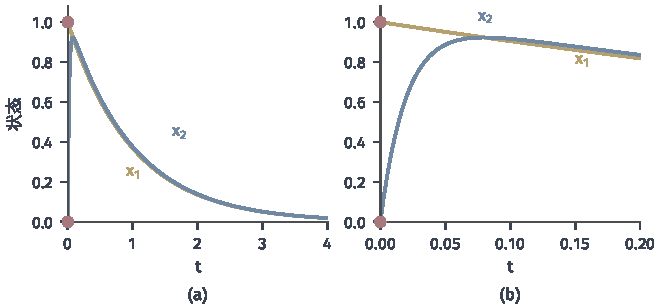
\includegraphics[width=112mm]{figures/06-differential-equations/01-ordinary-differential-equations/matplotlib/odenum-stiff-scales/figure.pdf}
 \caption{系统~\eqref{eq:odenum-stiff-system}的真解，蓝线为$x_2$，黄线为$x_1$，红点是初值。(a)整个区间，两条曲线在初始瞬间之后几乎重合。(b)放大开头的$t\in[0,0.2]$：$x_2$在大约$0.1$的时间内快速追上$x_1$。}
 \label{fig:odenum-stiff-scales}
\end{BookInlineFigure}

\paragraph{显式方法的步长限制}
对这个系统用显式Euler方法。$x_2$的更新是
\[
 x_2^{(k+1)}=(1-50h)\,x_2^{(k)}+50h\,x_1^{(k)}.
\]
括号里的$1-50h$是$x_2$的偏差每步被乘上的因子。$\lvert1-50h\rvert>1$时，偏差逐步放大，真解的平缓与否都救不了它。

取$h=0.05$，因子是$-1.5$，$x_2$的前几步是
\[
 2.5,\quad -1.375,\quad 4.319,\quad -4.335,
\]
而真解在$0.83$到$0.92$之间。取$h=0.03$，因子是$-0.5$，前几步是
\[
 1.5,\quad 0.705,\quad 1.059,\quad 0.840,
\]
逐渐稳定到真解附近（图~\ref{fig:odenum-stiff-euler}）。

\begin{BookInlineFigure}
 \centering
 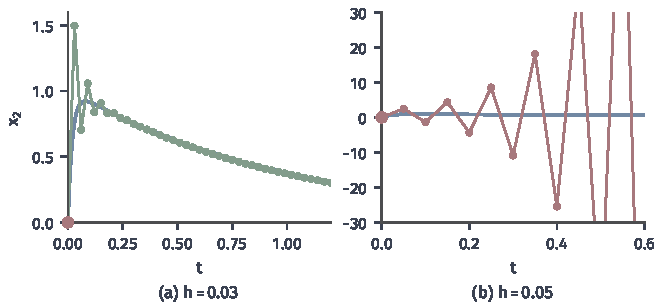
\includegraphics[width=112mm]{figures/06-differential-equations/01-ordinary-differential-equations/matplotlib/odenum-stiff-euler/figure.pdf}
 \caption{显式Euler方法用于系统~\eqref{eq:odenum-stiff-system}的$x_2$分量。蓝线是真解，红点是初值，折线是数值解。(a)$h=0.03$，一步因子$-0.5$，振荡衰减，绿线贴回真解。(b)$h=0.05$，一步因子$-1.5$，红线每步变号并放大。注意两图纵轴的范围不同。}
 \label{fig:odenum-stiff-euler}
\end{BookInlineFigure}

分界在$h=2/50=0.04$。这个限制来自早已衰减殆尽的快速分量，而不是来自要描绘的慢曲线。若把快速率从$50$提高到$5000$，步长上限就成了$4\times10^{-4}$，真解的慢曲线却没有任何变化。

像这样，稳定性对步长的要求比精度的要求严格得多的问题，称为\term{刚性问题}（stiff problem）。刚性没有一个公认的严格定义，它描述的是方程、方法和精度目标三者之间的关系：同一个方程，若目标就是精确刻画开头的快速过程，小步长是精度本身的需要，那就算不上刚性带来的麻烦。

第~\ref{sec:odenum-error-convergence}节的误差界在这里帮不上忙。系统的Lipschitz常数大约是$50$，定理~\ref{thm:odenum-global-error}的放大因子$\mathrm{e}^{\Lambda T}$在$T=4$时是$\mathrm{e}^{200}$量级。Lipschitz常数只看变化率的大小，看不出快速模式是在衰减还是在增长，所以需要另一种分析。

\subsection{绝对稳定性}
\label{sec:odenum-absolute-stability}

固定步长$h$，让步数不断增加，数值解中的扰动是衰减还是放大？回答这个问题的标准工具是一个最简单的方程。

\paragraph{测试方程与放大因子}
取标量线性方程，$\lambda$允许为复数，复数$\lambda$对应振荡的模式：
\begin{equation}
 \dot{x}=\lambda x,\qquad \lambda\in\mathbb{C}.
 \label{eq:odenum-test-equation}
\end{equation}
它称为\term{测试方程}（test equation）。对这个方程，一步方法每步把数值解乘上一个只依赖$z=h\lambda$的数$R(z)$，$R$称为方法的\term{放大因子}（amplification factor），也叫稳定函数。

逐个方法代入。显式Euler方法给出
\[
 x^{(k+1)}=x^{(k)}+h\lambda x^{(k)},
\]
所以$R(z)=1+z$。

中点方法的两个斜率分别是
\[
 k_1=\lambda x^{(k)},\qquad k_2=\lambda\Bigl(1+\frac{z}{2}\Bigr)x^{(k)},
\]
代入更新式$x^{(k+1)}=x^{(k)}+hk_2$，得到
\[
 R(z)=1+z+\frac{z^2}{2}.
\]

RK4的四个斜率依次为
\[
 \begin{aligned}
  k_1&=\lambda x^{(k)},\\
  k_2&=\lambda\Bigl(1+\frac{z}{2}\Bigr)x^{(k)},\\
  k_3&=\lambda\Bigl(1+\frac{z}{2}+\frac{z^2}{4}\Bigr)x^{(k)},\\
  k_4&=\lambda\Bigl(1+z+\frac{z^2}{2}+\frac{z^3}{4}\Bigr)x^{(k)}.
 \end{aligned}
\]
代入$\tfrac{h}{6}(k_1+2k_2+2k_3+k_4)$并合并同类项，得到
\[
 R(z)=1+z+\frac{z^2}{2}+\frac{z^3}{6}+\frac{z^4}{24}.
\]

三个放大因子都是$\mathrm{e}^{z}$的Taylor截断，截断的次数恰好等于方法的阶。真解每步被乘$\mathrm{e}^{z}$，$R(z)$就是对它的近似。

\begin{definition}[绝对稳定域]
 \label{def:odenum-stability-region}
 一步方法用于测试方程~\eqref{eq:odenum-test-equation}时若满足$x^{(k+1)}=R(z)x^{(k)}$，称
 \begin{equation}
  \bm{S}=\bigl\{z\in\mathbb{C}:\lvert R(z)\rvert\leq1\bigr\}
  \label{eq:odenum-stability-region}
 \end{equation}
 为方法的\term{绝对稳定域}（region of absolute stability）。
\end{definition}

当$\mathrm{Re}\,\lambda<0$时，测试方程的真解衰减，$\lvert\mathrm{e}^{z}\rvert<1$。我们希望数值解也不放大，这就要求$h\lambda$落在稳定域内。

\paragraph{从测试方程到线性系统}
为什么一个标量方程能说明系统的问题？设$\bm{A}$可对角化，$\bm{A}=\bm{V}\bm{D}\bm{V}^{-1}$。令$\bm{w}=\bm{V}^{-1}\bm{x}$，对显式Euler方法，
\[
 \bm{w}^{(k+1)}=(\bm{I}+h\bm{D})\bm{w}^{(k)},
\]
每个模式各自按测试方程演化。其他Runge--Kutta方法同样如此，因为它们都只用$\bm{A}$的多项式。

于是数值解不放大的条件是每个$h\lambda_i$都落在$\bm{S}$中。对系统~\eqref{eq:odenum-stiff-system}，$\lambda=-1$给出$z=-h$，$\lambda=-50$给出$z=-50h$；后者的约束才是起作用的。

\paragraph{稳定域的形状}
图~\ref{fig:odenum-stability-explicit}画出三个显式方法的稳定域。显式Euler方法的稳定域是以$-1$为心的单位圆盘，在负实轴上止于$-2$，这就是步长限制$h\leq2/\lvert\lambda\rvert$的来源。图中红点$z=-2.5$对应$h=0.05$，绿点$z=-1.5$对应$h=0.03$，与上面的计算一致。

\begin{BookInlineFigure}
 \centering
 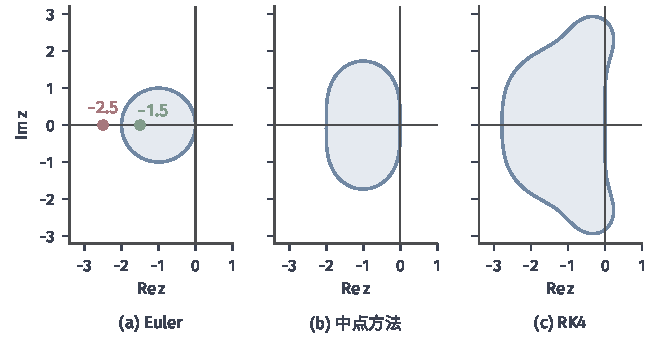
\includegraphics[width=112mm]{figures/06-differential-equations/01-ordinary-differential-equations/matplotlib/odenum-stability-explicit/figure.pdf}
 \caption{显式方法的绝对稳定域（浅蓝），边界是$\lvert R(z)\rvert=1$，三幅图的坐标范围相同。(a)显式Euler方法，红点$z=-2.5$在域外，绿点$z=-1.5$在域内；(b)中点方法，实轴上止于$-2$；(c)RK4，实轴上止于约$-2.785$。}
 \label{fig:odenum-stability-explicit}
\end{BookInlineFigure}

阶数提高，稳定域略有扩大，但RK4的实轴范围也只到约$-2.785$。原因在结构上：显式Runge--Kutta方法的$R(z)$总是多项式，当$\lvert z\rvert\to\infty$时$\lvert R(z)\rvert\to\infty$，所以稳定域必定有界。高阶的显式方法解除不了刚性带来的限制。

\paragraph{这一分析能说明什么}
测试方程分析的是数值扰动怎样传播，适用的情形是线性、常系数、矩阵可对角化，并且步长固定。在非线性问题上，通常把$\partial_{\bm{x}}\bm{f}$沿解冻结在某一时刻来做估计，这只是启发式的做法。它不能代替第~\ref{sec:odenum-error-convergence}节那样的收敛论证。

下面的时变系统说明冻结的特征值可能误导人。取矩阵
\[
 \bm{A}(t)=\begin{bmatrix}
  -1+\tfrac{3}{2}\cos^2t & 1-\tfrac{3}{2}\sin t\cos t\\
  -1-\tfrac{3}{2}\sin t\cos t & -1+\tfrac{3}{2}\sin^2t
 \end{bmatrix}.
\]
它的迹恒为$-1/2$，行列式恒为$1/2$，所以每个时刻的特征值都是$(-1\pm\mathrm{i}\sqrt{7})/4$，实部为$-1/4$，全在左半平面。

可是直接代入可以验证，下面的函数是方程$\dot{\bm{x}}=\bm{A}(t)\bm{x}$的解：
\[
 \bm{x}(t)=\mathrm{e}^{t/2}\begin{bmatrix}\cos t\\-\sin t\end{bmatrix},
\]
它的长度按$\mathrm{e}^{t/2}$增长（图~\ref{fig:odenum-frozen-coefficients}）。每一时刻看起来都是衰减的，解却在增长，因为特征方向在随时间转动。

\begin{BookInlineFigure}
 \centering
 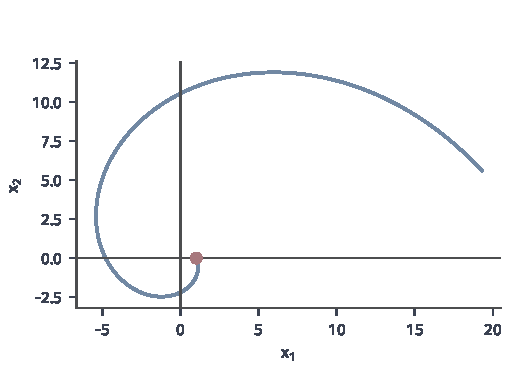
\includegraphics[width=86mm]{figures/06-differential-equations/01-ordinary-differential-equations/matplotlib/odenum-frozen-coefficients/figure.pdf}
 \caption{冻结特征值全在左半平面的时变线性系统。蓝线是从红点$(1,0)$出发的解，在$t\in[0,6]$上按$\mathrm{e}^{t/2}$向外旋转。}
 \label{fig:odenum-frozen-coefficients}
\end{BookInlineFigure}

\begin{BookInlineTable}
 \centering
 \caption{收敛与绝对稳定性的对比。}
 \label{tab:odenum-convergence-stability}
 \begin{tabular}{lll}
  \toprule
  & 收敛（定理~\ref{thm:odenum-global-error}） & 绝对稳定性\\
  \midrule
  关心的极限 & 固定$T$，$h\to0$ & 固定$h$，步数增加\\
  适用问题 & 非线性，有限区间 & 线性测试方程\\
  回答的问题 & 误差怎样随$h$减小 & 扰动是否放大\\
  \bottomrule
 \end{tabular}
\end{BookInlineTable}

\subsection{隐式格式}
\label{sec:odenum-implicit}

显式方法的放大因子是多项式，稳定域有界。要让稳定域覆盖整个左半平面，$R(z)$必须换成有理函数，这要求更新式的右端用到未知的新值。

\paragraph{主要思想}
回到积分式~\eqref{eq:odenum-integral-step}。Euler方法用左端点的值近似被积函数，现在改用右端点的值，得到\term{后向Euler方法}（backward Euler method）：
\begin{equation}
 \bm{x}^{(k+1)}=\bm{x}^{(k)}+h\,\bm{f}\bigl(t_{k+1},\bm{x}^{(k+1)}\bigr).
 \label{eq:odenum-backward-euler}
\end{equation}
未知的$\bm{x}^{(k+1)}$出现在等式两边，每一步都要解一个方程，这样的方法称为\term{隐式方法}（implicit method）。

把左右两端点的值平均，得到\term{梯形方法}（trapezoidal rule）：
\begin{equation}
 \bm{x}^{(k+1)}=\bm{x}^{(k)}+\frac{h}{2}\Bigl(\bm{f}\bigl(t_k,\bm{x}^{(k)}\bigr)+\bm{f}\bigl(t_{k+1},\bm{x}^{(k+1)}\bigr)\Bigr).
 \label{eq:odenum-trapezoid}
\end{equation}

在非刚性问题上它们的局部误差可以直接估计。对后向Euler方法，设$\bm{x}\in C^2$，$hL<1$，$\bm{y}=\bm{\Psi}_h(t_k,\bm{x}(t_k))$。真解满足同一个方程，只多一个余项$\bm{r}$，其大小满足
\[
 \lVert\bm{r}\rVert_2\leq\frac{h^2}{2}\max_{t}\lVert\ddot{\bm{x}}(t)\rVert_2.
\]
两式相减得到
\[
 \lVert\bm{y}-\bm{x}(t_{k+1})\rVert_2\leq hL\lVert\bm{y}-\bm{x}(t_{k+1})\rVert_2+\lVert\bm{r}\rVert_2,
\]
移项得到
\[
 \bigl\lVert\bm{\ell}^{(k+1)}\bigr\rVert_2\leq\frac{\lVert\bm{r}\rVert_2}{1-hL},
\]
所以后向Euler方法的阶是$1$。

梯形方法的阶是$2$，要求$\bm{x}\in C^3$：梯形求积公式的余项是$O(h^3)$，推导方式相同。这里的估计用了$hL<1$，刚性问题的$hL$很大，上面的估计就失去了意义，要靠下面的稳定性分析。

\paragraph{放大因子与稳定域}
把后向Euler方法用于测试方程，得到$x^{(k+1)}=x^{(k)}+zx^{(k+1)}$，解出
\begin{equation}
 R(z)=\frac{1}{1-z}.
 \label{eq:odenum-be-factor}
\end{equation}
于是$\lvert R(z)\rvert\leq1$等价于$\lvert1-z\rvert\geq1$，稳定域是以$1$为心的单位开圆盘的外部。

对梯形方法，同样的计算给出
\begin{equation}
 R(z)=\frac{1+z/2}{1-z/2}.
 \label{eq:odenum-trapezoid-factor}
\end{equation}
直接展开两个模的平方可得
\[
 \lvert1+z/2\rvert^2-\lvert1-z/2\rvert^2=2\,\mathrm{Re}\,z,
\]
所以$\lvert R(z)\rvert\leq1$恰好等价于$\mathrm{Re}\,z\leq0$，稳定域就是闭左半平面（图~\ref{fig:odenum-stability-implicit}）。

\begin{BookInlineFigure}
 \centering
 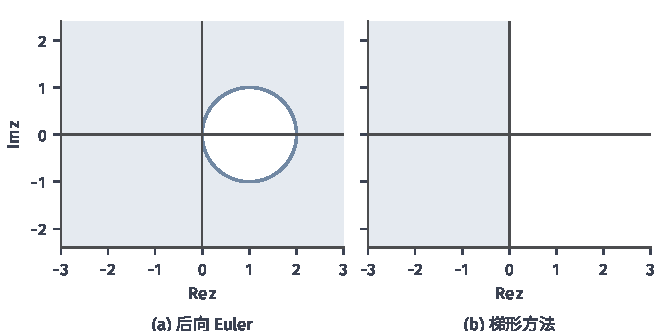
\includegraphics[width=112mm]{figures/06-differential-equations/01-ordinary-differential-equations/matplotlib/odenum-stability-implicit/figure.pdf}
 \caption{隐式方法的绝对稳定域（浅蓝）。(a)后向Euler方法，稳定域是以$1$为心的单位开圆盘（白色）的外部；(b)梯形方法，稳定域恰为闭左半平面。两者都包含闭左半平面，图中只画出有限范围。}
 \label{fig:odenum-stability-implicit}
\end{BookInlineFigure}

若稳定域包含闭左半平面，就称方法\term{A稳定}（A-stable）。这两个隐式方法都是A稳定的，因此用于系统~\eqref{eq:odenum-stiff-system}时不论$h$多大，线性模式都不会被放大。

\paragraph{快速模式的数值阻尼}
A稳定只保证不放大，不保证快速模式被迅速消除。比较$z\to-\infty$时的极限：真解的因子$\mathrm{e}^{z}\to0$，后向Euler的$R(z)\to0$，梯形方法的$R(z)\to-1$（图~\ref{fig:odenum-amplification-real}）。

\begin{BookInlineFigure}
 \centering
 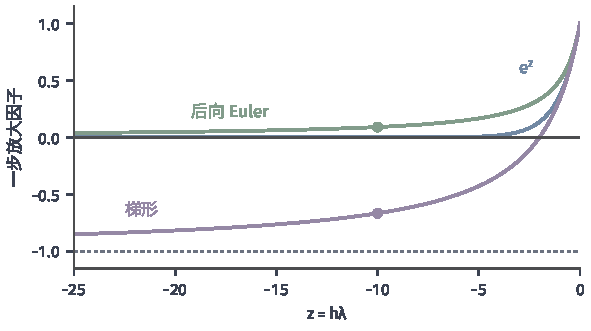
\includegraphics[width=100mm]{figures/06-differential-equations/01-ordinary-differential-equations/matplotlib/odenum-amplification-real/figure.pdf}
 \caption{负实轴上的一步放大因子。蓝线是真解的$\mathrm{e}^{z}$，绿线是后向Euler的$1/(1-z)$，紫线是梯形方法的$(1+z/2)/(1-z/2)$，灰色虚线是$-1$。圆点标出$z=-10$处的取值$1/11$和$-2/3$。}
 \label{fig:odenum-amplification-real}
\end{BookInlineFigure}

后向Euler对快速模式有很强的\term{数值阻尼}（numerical damping），模式一步就几乎消失。梯形方法的快速模式几乎不衰减，只是每步变号。在$z=-10$时，后向Euler的因子是$1/11$，梯形方法是$-2/3$。若方法既A稳定又满足$\lim_{z\to-\infty}R(z)=0$，就称方法\term{L稳定}（L-stable），后向Euler是，梯形方法不是。

\paragraph{计算过程：线性系统}
线性系统$\dot{\bm{x}}=\bm{A}\bm{x}$上，后向Euler方法每步解一个线性方程组，结果可以写成显式形式：
\begin{equation}
 \bm{x}^{(k+1)}=(\bm{I}-h\bm{A})^{-1}\bm{x}^{(k)}.
 \label{eq:odenum-be-linear}
\end{equation}
实际计算不求逆，而是分解一次$\bm{I}-h\bm{A}$再反复回代，步长不变时每步只需回代。下面用系统~\eqref{eq:odenum-stiff-system}演示，取$h=0.2$，它是显式方法上限$0.04$的五倍。

\needspace{6\baselineskip}
\paragraph{变量}
\begin{itemize}
 \item $\bm{x}^{(k)}\in\mathbb{R}^{n}$：第$k$个网格点的数值解。
 \item $\bm{I}-h\bm{A}\in\mathbb{R}^{n\times n}$：每步的系数矩阵，步长不变时只分解一次。
\end{itemize}

\paragraph{初始化}
把数值解初始化为初值，并构造系数矩阵。例中
\[
 \bm{x}^{(0)}=\begin{bmatrix}1\\0\end{bmatrix},\qquad
 \bm{I}-h\bm{A}=\begin{bmatrix}1.2&0\\-10&11\end{bmatrix}.
\]

\needspace{6\baselineskip}
\paragraph{每轮更新}
对$k=0,1,\ldots,N-1$依次执行：
\begin{enumerate}
 \item \textbf{求解第一个分量。}例中系数矩阵是下三角的，由第一行得到
 \[
  x_1^{(k+1)}=\frac{x_1^{(k)}}{1+h}.
 \]
 例中第一轮
 \[
  x_1^{(1)}=\frac{1}{1.2}=0.833333.
 \]
 \item \textbf{求解第二个分量。}由第二行得到
 \[
  x_2^{(k+1)}=\frac{x_2^{(k)}+50h\,x_1^{(k+1)}}{1+50h}.
 \]
 例中第一轮
 \[
  x_2^{(1)}=\frac{0+10\times0.833333}{11}=0.757576.
 \]
 例中第二轮，两个分量依次为
 \[
  x_1^{(2)}=0.694444,\qquad x_2^{(2)}=\frac{0.757576+6.944444}{11}=0.700184.
 \]
 \item \textbf{停止。}走满$N$步后结束。
\end{enumerate}
最终例中$t=0.4$处$x_2^{(2)}=0.700184$，真值约为$0.684000$，没有振荡。第一步的误差较大，因为$h=0.2$完全跨过了快速过渡，这是用一步盖过快速过程的代价，后面的步很快贴回真解。

图~\ref{fig:odenum-implicit-stiff}比较两种隐式方法。梯形方法的第一轮为
\[
 x_2^{(1)}=\frac{5\,(x_1^{(0)}+x_1^{(1)})-4\,x_2^{(0)}}{6}=1.515152,
\]
其中$x_1^{(1)}=0.818182$。它明显越过真解，之后按因子$-2/3$交替变号衰减，正好体现了图~\ref{fig:odenum-amplification-real}中$z=-10$处的差别。

\begin{BookInlineFigure}
 \centering
 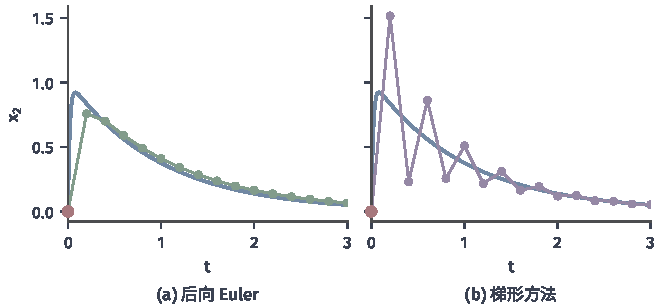
\includegraphics[width=112mm]{figures/06-differential-equations/01-ordinary-differential-equations/matplotlib/odenum-implicit-stiff/figure.pdf}
 \caption{隐式方法用于系统~\eqref{eq:odenum-stiff-system}，$h=0.2$，纵轴为$x_2$。蓝线是真解，红点是初值。(a)后向Euler方法（绿）没有振荡；(b)梯形方法（紫）第一步越过真解，之后交替变号衰减。}
 \label{fig:odenum-implicit-stiff}
\end{BookInlineFigure}

\paragraph{计算过程：非线性方程}
非线性问题的隐式更新没有闭式，需要迭代。对后向Euler方法，设$\bm{y}$是要求的$\bm{x}^{(k+1)}$，解方程
\begin{equation}
 \bm{G}(\bm{y})=\bm{y}-\bm{x}^{(k)}-h\,\bm{f}(t_{k+1},\bm{y})=\bm{0}.
 \label{eq:odenum-implicit-equation}
\end{equation}

最直接的不动点迭代$\bm{y}\leftarrow\bm{x}^{(k)}+h\bm{f}(t_{k+1},\bm{y})$只在$hL<1$时保证压缩，这恰好是显式方法的步长量级，隐式方法的好处就丢掉了。所以刚性问题通常用Newton迭代，即每次解线性方程组
\[
 \bigl(\bm{I}-h\,\partial_{\bm{x}}\bm{f}(t_{k+1},\bm{y})\bigr)\bm{\Delta}=-\bm{G}(\bm{y}),
\]
再令$\bm{y}\leftarrow\bm{y}+\bm{\Delta}$。Newton法的收敛性质可参考\BookChapterRef{chap:second-order-methods}{卷五第7章“二阶方法”}，线性方程组的分解可参考\BookChapterRef{chap:direct-linear-solvers}{卷二第12章“线性方程的直接求解”}。

用例~\eqref{eq:odenum-running}演示，$h=0.5$。一维时
\[
 G(y)=y-x^{(k)}-0.5\,y(1-y),\qquad G'(y)=1-0.5(1-2y).
\]
以显式Euler的结果$y=0.28$作初值，第一步的迭代为
\[
 G(0.28)=-0.0208,\quad G'(0.28)=0.78,\quad y=0.306667.
\]
第二次迭代得到
\[
 G(0.306667)=3.56\times10^{-4},\quad G'(0.306667)=0.806667,\quad y=0.306226.
\]
此时$\lvert G\rvert$已降到$10^{-7}$量级，取$x^{(1)}=0.306226$。

\paragraph{内部容差计入误差预算}
隐式更新解不到严格的零。迭代提前停止留下的偏差，正是式~\eqref{eq:odenum-computed}中的计算误差$\bm{\delta}^{(k+1)}$。由定理~\ref{thm:odenum-global-error}，它在全局误差中贡献$\varepsilon/h$的量级。

图~\ref{fig:odenum-inner-tolerance}给出一个实验：对例~\eqref{eq:odenum-running}用梯形方法，内部用不动点迭代（此处$h$较小，迭代是压缩的），当相邻两次迭代之差不超过内部容差时停止。容差很小时，误差停在由截断决定的平台；容差放松到一定程度，误差会阶梯式上升，最宽松时一次迭代就停，格式退化为一阶。

\begin{BookInlineFigure}
 \centering
 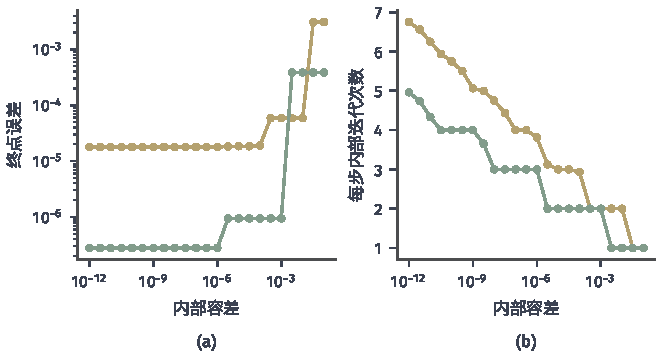
\includegraphics[width=112mm]{figures/06-differential-equations/01-ordinary-differential-equations/matplotlib/odenum-inner-tolerance/figure.pdf}
 \caption{内部方程的容差对梯形方法的影响，问题为式~\eqref{eq:odenum-running}，$T=1$，内部采用不动点迭代。黄线$N=16$，绿线$N=128$。(a)终点误差：容差小时不随容差变化，容差大时误差阶梯式上升。(b)每步平均内部迭代次数：容差越小迭代越多。}
 \label{fig:odenum-inner-tolerance}
\end{BookInlineFigure}

这个实验给出的预算原则是：内部容差要明显小于这一步允许的局部误差，否则花在高阶公式上的计算会被内部误差抵消；反过来把容差压得远低于截断误差，只是白白增加迭代次数。

\paragraph{不能只看阶数}
选择方法时要同时考虑稳定域、每步求解代价和计算误差。对系统~\eqref{eq:odenum-stiff-system}，RK4虽然是四阶，步长仍受$2.785/50\approx0.056$的限制，走到$T=4$至少$72$步、$288$次右端求值。一阶的后向Euler方法取$h=0.2$只需$20$步，每步解一次$2\times2$的线性方程组，而且不会发散。

反过来，方程若不刚性，隐式方法每步要解方程，就比显式方法贵得多，也得不到额外好处。表~\ref{tab:odenum-implicit-compare}汇总本节的方法。

\begin{BookInlineTable}
 \centering
 \caption{显式与隐式方法的对比，$z=h\lambda$。}
 \label{tab:odenum-implicit-compare}
 \begin{tabular}{llcc}
  \toprule
  方法 & $R(z)$ & 阶 & A稳定\\
  \midrule
  显式Euler & $1+z$ & 1 & 否\\
  RK4 & 四次多项式 & 4 & 否\\
  后向Euler & $1/(1-z)$ & 1 & 是，$R(-\infty)=0$\\
  梯形 & $(1+z/2)/(1-z/2)$ & 2 & 是，$R(-\infty)=-1$\\
  \bottomrule
 \end{tabular}
\end{BookInlineTable}


\section{自适应步长}
\label{sec:odenum-adaptive}

固定步长要在全程迁就最难走的一段。解在某处急转，别处平缓，均匀的小步长就是浪费，均匀的大步长又不够准。程序能不能边走边判断，自己决定每一步走多远？

\paragraph{主要思想：估计局部误差}
要调节步长，先要知道这一步的误差有多大。真解未知，但可以用两个不同精度的结果相减来估计。

一种办法是\term{步长加倍}（step doubling）。设方法的阶为$p$，从同一点出发，用步长$h$走一步得到$\bm{y}_1$，用步长$h/2$走两步得到$\bm{y}_2$。忽略高阶项，两者的误差主要部分分别是$\bm{c}h^{p+1}$和$2\bm{c}(h/2)^{p+1}$，相减消去未知的真解，得到对$\bm{y}_2$的误差估计
\begin{equation}
 \bm{x}(t+h)-\bm{y}_2\approx\frac{\bm{y}_2-\bm{y}_1}{2^{p}-1}.
 \label{eq:odenum-step-doubling}
\end{equation}

例~\eqref{eq:odenum-running}的第一步，Euler方法用$h=0.5$得$0.28$，用两个$0.25$的半步得$0.2856$，由式~\eqref{eq:odenum-step-doubling}估计真解比$0.2856$约大$0.0056$。实际差是$0.291875-0.2856=0.0063$，估计相当准确。这种做法要多算一倍的步，代价偏高。

另一种办法用同一组阶段斜率组合出两个不同阶的结果，它们的差就是误差估计，不增加右端求值，这样的方法称为\term{嵌入式Runge--Kutta方法}（embedded Runge--Kutta method）。最简单的例子是Heun--Euler对。

取Heun方法的两个斜率$\bm{k}_1=\bm{f}(t,\bm{x})$，$\bm{k}_2=\bm{f}(t+h,\bm{x}+h\bm{k}_1)$。一阶的结果只用$\bm{k}_1$，二阶的结果用两者平均：
\[
 \bm{x}_{\mathrm{low}}=\bm{x}+h\bm{k}_1,\qquad
 \bm{x}_{\mathrm{high}}=\bm{x}+\frac{h}{2}(\bm{k}_1+\bm{k}_2).
\]
两者之差估计低阶结果的误差：
\begin{equation}
 \bm{d}=\bm{x}_{\mathrm{high}}-\bm{x}_{\mathrm{low}}=\frac{h}{2}(\bm{k}_2-\bm{k}_1).
 \label{eq:odenum-embedded-estimate}
\end{equation}
实际使用的是更高阶的配对，例如Dormand--Prince的五四阶方法\scite{math-hairer1993ode}，原理相同。

\paragraph{主要思想：尺度、接受与新步长}
误差估计要和一个容许的尺度比较。各分量量纲可能不同，大小也可能相差很多，所以给每个分量一个尺度，同时用\term{绝对容差}（absolute tolerance）$\eta_{\mathrm{a}}$和\term{相对容差}（relative tolerance）$\eta_{\mathrm{r}}$：
\begin{equation}
 w_i=\eta_{\mathrm{a}}+\eta_{\mathrm{r}}\max\bigl\{\lvert x_i\rvert,\ \lvert x_{\mathrm{high},i}\rvert\bigr\}.
 \label{eq:odenum-scale}
\end{equation}
相对容差让大分量按比例控制精度；绝对容差防止分量接近零时尺度也趋于零，把步长压到不合理的小。

归一化的误差取各分量比值的最大值：
\begin{equation}
 \mathrm{err}=\max_{i}\frac{\lvert d_i\rvert}{w_i}.
 \label{eq:odenum-err}
\end{equation}
若$\mathrm{err}\leq1$，这一步被接受，否则放弃这一步，用更小的步长重算。

无论接受与否，都要决定下一个步长。低阶结果的阶为$q$时，$\mathrm{err}$大约正比于$h^{q+1}$，要让它变成$1$，步长应乘以$\mathrm{err}^{-1/(q+1)}$。加上安全系数$\gamma<1$和增减幅度的限制，得到
\begin{equation}
 h_{\mathrm{new}}=h\,\min\Bigl\{f_{\max},\ \max\bigl\{f_{\min},\ \gamma\,\mathrm{err}^{-1/(q+1)}\bigr\}\Bigr\}.
 \label{eq:odenum-step-control}
\end{equation}
限制幅度是因为$\mathrm{err}$只是估计，步长剧烈变化会使估计失效。

\paragraph{计算过程}
下面用例~\eqref{eq:odenum-running}演示Heun--Euler对，$q=1$，取容差和控制参数为
\[
 \eta_{\mathrm{a}}=\eta_{\mathrm{r}}=10^{-3},\quad\gamma=0.9,\quad f_{\min}=0.2,\quad f_{\max}=5,
\]
初始步长取$h=0.5$，积分到$T=1$，接受后沿用高阶结果继续。

\needspace{6\baselineskip}
\paragraph{变量}
\begin{itemize}
 \item $t$，$\bm{x}\in\mathbb{R}^{n}$：已接受的当前时刻和数值解。
 \item $h$：当前尝试的步长。
 \item $\bm{k}_1,\bm{k}_2\in\mathbb{R}^{n}$：本次尝试的两个阶段斜率。
 \item $\bm{d}$，$\mathrm{err}$：误差估计和归一化误差。
 \item 标记$\mathrm{failed}$：上一次尝试是否被拒绝，被拒绝后下一步的$f_{\max}$取$1$，避免紧接着又放大步长。
\end{itemize}

\paragraph{初始化}
把当前点初始化为初值，并设初始步长。例中
\[
 t=0,\qquad x=0.2,\qquad h=0.5,\qquad \mathrm{failed}=\text{否}.
\]

\needspace{6\baselineskip}
\paragraph{每轮更新}
当$t<T$时重复：
\begin{enumerate}

 \item \textbf{截断到终点。}令$h\leftarrow\min\{h,T-t\}$，保证不越过$T$。

 \item \textbf{算两个斜率和两个结果。}计算$\bm{k}_1,\bm{k}_2$，$\bm{x}_{\mathrm{high}}$，并由式~\eqref{eq:odenum-embedded-estimate}算$\bm{d}$。例中第一次尝试
 \[
  k_1=0.16,\qquad k_2=f(0.28)=0.2016,
 \]
 于是
 \[
  x_{\mathrm{high}}=0.2904,\qquad d=0.25\times0.0416=0.0104.
 \]

 \item \textbf{比较尺度。}由式~\eqref{eq:odenum-scale}和式~\eqref{eq:odenum-err}计算$\mathrm{err}$。例中第一次尝试
 \[
  w=10^{-3}+10^{-3}\times0.2904=0.00129,\qquad \mathrm{err}=8.06.
 \]

 \item \textbf{接受或拒绝。}若$\mathrm{err}\leq1$，令$t\leftarrow t+h$，$\bm{x}\leftarrow\bm{x}_{\mathrm{high}}$，$\mathrm{failed}$置为否；否则状态不变，$\mathrm{failed}$置为是。例中第一次$\mathrm{err}>1$，拒绝，状态仍为$(0,\,0.2)$。

 \item \textbf{更新步长。}由式~\eqref{eq:odenum-step-control}计算$h_{\mathrm{new}}$，令$h\leftarrow h_{\mathrm{new}}$。例中第一次尝试
 \[
  h_{\mathrm{new}}=0.5\times\max\bigl\{0.2,\ 0.9\times8.06^{-1/2}\bigr\}=0.5\times0.317=0.1585.
 \]
 例中第二次尝试用$h=0.1585$，得到
 \[
  k_2=0.174574,\qquad x_{\mathrm{high}}=0.226517,\qquad \mathrm{err}=0.942,
 \]
 这一步被接受，$t$更新为$0.1585$，$x$更新为$0.226517$。

 \item \textbf{停止。}当$t=T$时结束。
\end{enumerate}
全程的尝试列于表~\ref{tab:odenum-adaptive-trace}。一共$8$次尝试、$16$次右端求值，一次被拒绝；最终$x=0.404269$，真值$0.404610$，全局误差$-3.4\times10^{-4}$。

\begin{BookInlineTable}
 \centering
 \caption{Heun--Euler对在式~\eqref{eq:odenum-running}上的步长控制，$\eta_{\mathrm{a}}=\eta_{\mathrm{r}}=10^{-3}$。最后一步被截断以恰好到达$T=1$。}
 \label{tab:odenum-adaptive-trace}
 \begin{tabular}{rrrrc}
  \toprule
  $t$ & $h$ & $x_{\mathrm{high}}$ & $\mathrm{err}$ & 结果\\
  \midrule
  0 & 0.50000 & 0.290400 & 8.060 & 拒绝\\
  0 & 0.15851 & 0.226517 & 0.942 & 接受\\
  0.15851 & 0.14701 & 0.253260 & 0.787 & 接受\\
  0.30552 & 0.14911 & 0.282437 & 0.763 & 接受\\
  0.45462 & 0.15366 & 0.314545 & 0.735 & 接受\\
  0.60828 & 0.16128 & 0.350259 & 0.698 & 接受\\
  0.76956 & 0.17373 & 0.390689 & 0.642 & 接受\\
  0.94329 & 0.05671 & 0.404269 & 0.056 & 接受\\
  \bottomrule
 \end{tabular}
\end{BookInlineTable}

\paragraph{步长怎样跟随解}
图~\ref{fig:odenum-adaptive-steps}是同一控制器用在变化更剧烈的方程$\dot{x}=12x(1-x)$上的结果，$x(0)=0.02$，容差仍为$10^{-3}$。解从缓慢上升到快速爬升，再到贴近平衡点。控制器在曲线转弯的区域用小步，在平衡点附近把步长放大，共接受$49$步、拒绝$6$步，$110$次右端求值，终点误差约$5\times10^{-4}$。

\begin{BookInlineFigure}
 \centering
 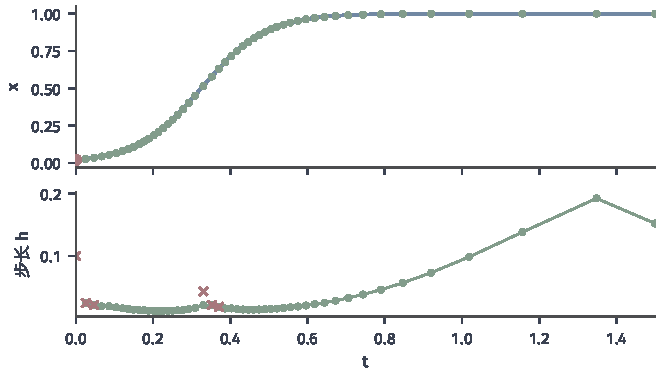
\includegraphics[width=112mm]{figures/06-differential-equations/01-ordinary-differential-equations/matplotlib/odenum-adaptive-steps/figure.pdf}
 \caption{自适应步长跟随解的变化，方程$\dot{x}=12x(1-x)$，$x(0)=0.02$，$\eta_{\mathrm{a}}=\eta_{\mathrm{r}}=10^{-3}$。上图蓝线是真解，红点是初值，绿点是接受的网格值；下图绿线是接受步的步长，红叉是被拒绝的尝试。}
 \label{fig:odenum-adaptive-steps}
\end{BookInlineFigure}

\paragraph{局部容差不直接保证全局精度}
控制器管的是每一步新增的偏差，全局误差还要乘上流映射的放大。回到第~\ref{sec:odenum-time-discretization}节的方程$\dot{x}=\sigma(x-\cos t)-\sin t$，$x(0)=1$，积分到$T=2$。图~\ref{fig:odenum-adaptive-global}显示，同样的局部容差，$\sigma=-5$时全局误差大致等于容差，$\sigma=5$时放大了四个多数量级。容差取$10^{-5}$时，前者的全局误差约$6\times10^{-6}$，后者约$0.18$。

\begin{BookInlineFigure}
 \centering
 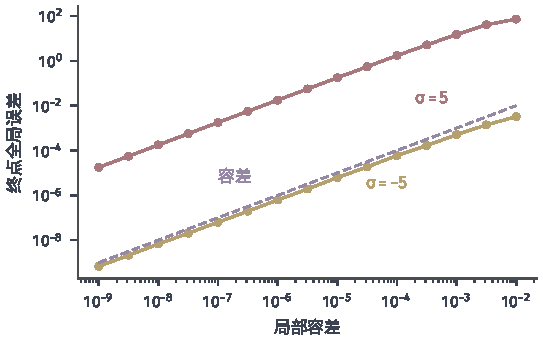
\includegraphics[width=92mm]{figures/06-differential-equations/01-ordinary-differential-equations/matplotlib/odenum-adaptive-global/figure.pdf}
 \caption{局部容差与终点全局误差，方程为$\dot{x}=\sigma(x-\cos t)-\sin t$，$x(0)=1$，$T=2$，$\eta_{\mathrm{a}}=\eta_{\mathrm{r}}$。黄线$\sigma=-5$，红线$\sigma=5$，紫色虚线为容差本身。}
 \label{fig:odenum-adaptive-global}
\end{BookInlineFigure}

所以容差不是全局精度的保证。可靠的做法是把容差减小一两个数量级再解一次，比较两次的结果；或者用第~\ref{chap:ode-sensitivity}章的敏感性信息估计放大因子。这样的比较检验的是数值误差，并不能发现模型本身的错误。

\paragraph{自适应不能解决刚性}
控制器还会被稳定性牵着走。把Heun--Euler对用于系统~\eqref{eq:odenum-stiff-system}，容差$10^{-3}$，走到$T=4$。快速过渡结束后，解已经很平缓，局部误差估计却不断地“被激发”：一旦步长越过稳定上限，快速模式开始放大，误差估计变大，步长又被压回来。

结果是步长一直贴着上限$2/50$上下摆动（图~\ref{fig:odenum-adaptive-stiff}）。共接受$141$步、拒绝$13$步，$308$次右端求值，后半程的平均步长约$0.039$，而精度本来允许走得更远。

\begin{BookInlineFigure}
 \centering
 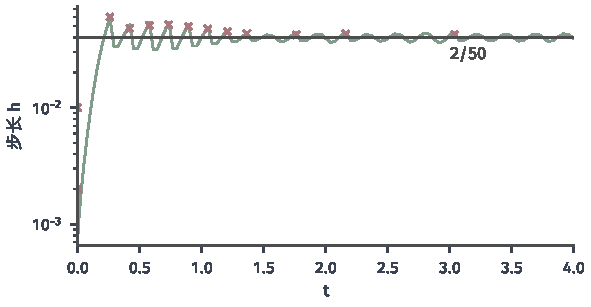
\includegraphics[width=100mm]{figures/06-differential-equations/01-ordinary-differential-equations/matplotlib/odenum-adaptive-stiff/figure.pdf}
 \caption{显式嵌入对用于刚性系统~\eqref{eq:odenum-stiff-system}时的步长历史，容差$10^{-3}$。绿线是接受步的步长，红叉是被拒绝的尝试，深灰线是稳定上限$2/50$。解变平缓之后，步长仍被稳定性限制。}
 \label{fig:odenum-adaptive-stiff}
\end{BookInlineFigure}

步长长期贴着一个与解的光滑程度无关的水平，同时反复被拒绝，这本身就是刚性的信号，应当换成隐式方法。求值次数的增长同样值得监控：它比预期多很多时，要么是方程刚性，要么是右端有不连续点，控制器把步长压小只是在逼近那一点，并不能恢复方法的阶。


\section{本章小结}
\label{sec:odenum-summary}

本章回答了开头的三个问题。怎样走一步：所有方法都在近似积分式~\eqref{eq:odenum-integral-step}，显式Euler方法只看起点，Runge--Kutta方法在一步内多次采样并匹配Taylor展开，隐式方法把未知的终点也放进来。

误差怎样累积：局部截断误差沿真解定义，没有除以步长。定理~\ref{thm:odenum-global-error}说明，在解存在的有限区间上，只要方法一步稳定、一步误差一致地是$O(h^{p+1})$、初值误差和计算误差足够小，全局误差就是$O(h^{p})$。它的常数含有$\mathrm{e}^{\Lambda T}$，这是有限时间的结论，不描述长期行为。

步长由什么决定：非刚性问题由精度决定，刚性问题由稳定性决定。绝对稳定域回答固定步长下扰动是否放大，它基于线性测试方程，不能代替一般的收敛论证。

表~\ref{tab:odenum-choice}按问题的特点比较代表方法。

\begin{BookInlineTable}
 \centering
 \caption{方法选择的对比。}
 \label{tab:odenum-choice}
 \begin{tabular}{p{28mm}p{30mm}p{36mm}}
  \toprule
  问题特点 & 适用方法 & 主要代价或风险\\
  \midrule
  光滑，非刚性，低精度 & 低阶显式方法 & 精度要求提高时成本急增\\
  光滑，非刚性，高精度 & RK4或高阶嵌入对 & 需要足够的光滑性\\
  右端有已知跳变 & 在跳变点分段积分 & 不分段时阶数丢失\\
  刚性 & 后向Euler等隐式方法 & 每步解方程，内部容差计入预算\\
  解的尺度变化大 & 自适应步长 & 容差不等于全局精度\\
  \bottomrule
 \end{tabular}
\end{BookInlineTable}

两种常用的检验要分清。步长细化比较不同步长的结果，能观察实际的收敛阶，发现阶数丢失和舍入误差主导，但要求解在相应步长上已进入渐近范围。局部误差估计只度量一步新增的偏差，不包含累积，也察觉不到系统性的模型错误。

偏微分方程在空间离散后成为大型常微分方程组，时间推进可以直接使用本章的方法，空间网格越细，系统通常越刚性，具体分析见第~\ref{chap:pde-numerical-methods}章。长时间积分时的结构保持、吸引子等离散动力学问题超出了有限区间收敛定理的范围，可参考\BookChapterRef{chap:dynamical-systems-long-term}{卷九第1章“动力系统与轨迹的长期行为”}。


